
\RequirePackage{marginnote}
%\let\marginpar\marginnote
\let\marginnote\undefined

\documentclass[a4paper, notoc, justified,marginals=left, nobib]{tufte-book}


\usepackage[utf8]{inputenc}
\usepackage{graphicx} % allow embedded images
  \setkeys{Gin}{width=\linewidth,totalheight=\textheight,keepaspectratio}
  \graphicspath{{graphics/}} % set of paths to search for images
\usepackage{amsmath}  % extended mathematics
\usepackage{booktabs} % book-quality tables
\usepackage{units}    % non-stacked fractions and better unit spacing
\usepackage{multicol} % multiple column layout facilities
\usepackage{fancyvrb} % extended verbatim environments
  \fvset{fontsize=\normalsize}% default font size for fancy-verbatim environments
\usepackage{pgfplots}
% The following package makes prettier tables.  We're all about the bling!
\usepackage{booktabs}


% Make glossary
\usepackage[nonumberlist,toc,nopostdot,style=tree]{glossaries}

\usepackage{lipsum}
\usepackage{hyperref}

\usepackage{pdfpages} % insert the papers pdf in the text.

\usepackage{gensymb} %°C


 \usepackage{lscape}   % paysage
 \usepackage{pdflscape,array,booktabs}%pages du pdf avec tableau en paysage
 
% get rid of page numbers in TOC
%\usepackage{tocloft}
%\cftpagenumbersoff{part}
%\cftpagenumbersoff{chapter}
%\cftpagenumbersoff{section}

% make footnotes and sidenotes counters be reset per page
\usepackage{perpage} %the perpage package
\MakePerPage{footnote} %the perpage package command
\MakePerPage{sidenote} %the perpage package command

% create an index
\usepackage{makeidx}
% Tells latex to make an index
\makeindex


%% for proper citation styling
%\usepackage{natbib}
%\setcitestyle{authoryear}

% for split bibliography
%\usepackage[sorting=nyt, style = authoryear,url = false, doi = false, isbn = false, backend=biber]{biblatex}
\usepackage[sorting=nyt,style = authoryear,bibencoding=auto,url = false, doi = false, isbn = false,backend=biber,natbib]{biblatex} % alternative bibliography


\renewbibmacro{in:}{%
  \ifentrytype{article}{}{\printtext{\bibstring{in}\intitlepunct}}}

%\usepackage{natbib}
%\setcitestyle{authoryear}


 %\addbibresource{../Bibliography/bib_zotero20171106.bib}
 \addbibresource{../Bibliography/bib_zotero20180615.bib}
 \addbibresource{../Bibliography/bib_zotero_update_20180615_20180712.bib}
%\includeonly{./2_PP/Individual_level, ./2_PP/Community_dynamics}
%\includeonly{./0_Objectives/Objectives, ./1_Introduction/Introduction}

%
%\chapter{Objectives}

\chapter{Context}

\section{Global change: how to describe the future of alpine ecosystems?}

\subsection{The value of ecosystems: from properties to services}

\paragraph{A new logic}
Everyone has a particular relationship with nature. The vision we put behind this word depends on the way we experienced nature, it can be temperate or tropical forest, mountain rivers or cliffs on the ocean littoral, bird songs or wind between stones. Anybody that shares one of these visions, I am sure wants to preserve natural systems. But facing this emotional perception and inner desire to see these ecosystems be preserved, other forces pushes in other directions. The reduction of biodiversity is increasing at dangerous rates, the deforestation threaten the largest forest systems, insects are less and less presents and animals are repelled to fragmented and diminishing habitats. Other logics than emotional attachment and will to protect impact all natural systems around the world. To be protected, the natural systems needed a way to be integrated in these logics, and the notion of \textemph{ecosystem services} was developed by \cite{costanza_value_1997}. This notion encompass all benefits human extract from ecosystems. It enables a categorisation of services and their quantification (that can go to the monetisation), and therefore allow them to be taken into consideration in global logic of capital, investment and value.


\paragraph{Services}
The notion of ecosystem services aims to capture the value of ecosystem, but what is this value?

If ones could be tempted to answer that the value of an ecosystem cannot be measures, it is clear that all ecosystems do not benefit to human in the same way. Face to the diversity of ecosystems and services they provide, we can try to develop a short answer for the object of study to this document: mountain grasslands.

\textemph{Mountain grasslands} designs in this document all grasslands, below and above the treeline, that have short growing seasons delimited by snow covered periods and experience high variations in temperature and water availability. This term is intentionally generic as the scope of this work is relatively broad and theoretical.

Mountain grasslands provide numerous services, that can be divided in multiple categories such as provision, cultural and regulating services. Provision services are related to the quantity and quality of primary resources the grasslands provide. Fodder production and quality are the main measures of provision services. Other services can be included in this category: diversity of flowers and phenology for flower production for instance. Productivity is also interesting to assess carbon capture, a regulating service. Soil nutrient availability and water filtering are other regulating services impacted by the identity and diversity of species populating mountain grasslands. Finally, cultural services, related to tourism activity and landscape appeal are also related to grasslands species diversity.


In case of terrestrial ecosystems, vegetation cover is often central because of: it role of primary production, and the fact that vegetation community informs a lot on the properties of the abiotic and biotic conditions. Moreover, a most of studies on services from terrestrial ecosystem are interested in plants and soil invertebrate \cite{de_bello_towards_2010}, revealing the importance of vegetation in the provision of ecosystem services. In addition, in alpine habitats plant communities are susceptible to be the first impacted by global change because they cannot escape changes in conditions and are the target of management practices linked to fodder productions. All these arguments support the interest of studying the vegetation dynamics for the assessment of ecosystem services.

\begin{figure*}
\includegraphics{./1_Introduction/graphics/alpine_distribution.jpeg}
\caption{Distribution of alpine habitats. Alpine habitats shelter unique and rich ecosystems providing numerous services to human populations. Climate change and mutations of land-use practices threaten these dispersed and fragile habitats.}
\end{figure*}

\paragraph{Properties}
The ecosystem services are tightly related to the \textemph{ecosystem properties} (as illustrated in figures \ref{fig:properties})\parencite{lavorel_predicting_2002, diaz_incorporating_2007} that can be extracted from the description of the grassland communities. Ecosystem properties are features of the community that characterise it and arise from the characteristics of all parts of  the system or how they combine. The main properties of a plant community are capture in the following concepts:
\begin{itemize}
\item \textemph{identity}: the identity of the community refers to the dominant species (or directly its characteristics) of the community that transfers its traits to the whole community. It can also refer to mean traits (with community weighted mean measures) of a community. In this document, identity will often be used to talk about the resource use strategy (more or less exploitative). While this notion can encompass multiple traits and measures, it is practical to use one term to identify components of the community description that can be attributed to a species\sidenote{in opposition to variables that are related to a system, \textit{e.g.} diversity cannot be expressed for a species alone};
\item \textemph{diversity}: diversity plays a large role in the provision of multiple services, and is related to other properties of the community. Diversity can be expressed in term of species richness or functional diversity\sidenote{each measure depending on the functional space that is considered}, and by a wide range of indexes that are not discussed here. Despite a lot of nuances between these notions, they are often tightly correlated and diversity will be discussed in term of number of species or functional volume in the rest of this document.
\item \textemph{productivity}: productivity captures the capacity of the system to produce organic matter in a given timespan. It is a ambiguous term as it can refer to the abiotic environment, to a species or a community property or even to a service. I will try to limit its use to the species or community relative vegetative biomass in a given condition.
\end{itemize}

%-----------------------------------------------------------------------------------------
%\subsection{From community description to ecosystem services: the facets of the community}

%Ecosystem services are various. Some of them can be easily assess (e.g. fooder production and quality), while others are more subjective (cultural or recreational services) or hard to measure (carbon sequestration, water purification etc...). But all of them rely on a good description of the system, even though this description do not have to be complete as certain aspect of an ecosystem might not be relevant to all provided services.


Linking ecosystem services to ecosystem properties is essential both for the understanding of processes controlling these services, and for an easier quantification of such services. This is particularly important for the prediction of services levels to plan management practices in the context of global change. Some ecosystem services are here linked to the main community properties as illustrated in figure  \ref{fig:properties}.
% The question of the description and prediction of plant communities properties and dynamics will be addressed more in details in the following sections of this chapter, but it is important to establish the main components of a vegetation community link with provided services.


\paragraph{Diversity}


\paragraph{Identity}

\paragraph{Productivity}
Mountain grasslands provide numerous ecosystem services 

ecosystem services depends on abiotic, but also biotic factors and properties. 

%
%%-----------------------------------------------------------------------------------------
%\subsection{The facets of plant communities}

%

%The assessment of ecosystem services relies on a detailed characterisation of the community structure and properties. The knowledge of species characteristics and relative abundance allows the computation of summary variables that characterise the plant community. Long history of plant study and description gives us good knowledge of benefit provided by specific species. 

This structure is defined by the relative abundance of the different species of the community. Multiple drivers affect the relative abundance of a given species, from abiotic filtering processes to biotic interactions. 

Need of mechanisms to produce dynamics and give properties.

\textbf{The complexity of plant community dynamics requires mechanistic approaches to understand and predict system properties in new, extreme, and variable conditions. }


\textbf{The evaluation of ecosystem services relies on a precise description of the ecosystem abiotic and biotic properties. The plant community is the most dynamic and complex driver of ecosystem services, but direct links can be drawn between the fine description of the community and the ecosystem services. Understanding and prediction the main variables dynamics that capture those links is necessary to efficiently predict changes in ecosystem services levels.}
\textbf{Plant communities are complex interconnected systems. In order to evaluate ecosystem services, they can be summarised by three main types of variables that capture different dimensions of such systems: the diversity, the productivity and the identity. These dimensions can be studied independently or jointly and give different information on secondary properties and provided services. But grassland communities are natural systems driven by environmental variables, and these drivers are changing leading to changes in services.}



\subsection{Global change: what changes and what consequences}

Mountain grasslands are maintained by strong climatic constraints that limit growth rate and lifeforms  \parencite{koorner_alpine_2003}, but also frequent grazing or cutting perturbation regimes that strongly limit the growth woody species and favour low stature species or rapid growth herbs \parencite{diaz_plant_2007}. But these drivers are changing at alarming rates and mountain grasslands are suspected to be very vulnerable \parencite{engler_21st_2011} due to higher variations in water availability regimes and specific warming processes \parencite{mountain_research_initiative_edw_working_group_elevation-dependent_2015}, stronger isolation (island effect due to rise in temperature) and reduction of the grazing pressure.

\paragraph{Climate change}
Changes:
Rising temperatures due to anthropogenic greenhouse gases has a strong effect on mountain climate. 

Consequences: contrasting, depends on the factor: co2 or drought

\paragraph{Land-use mutations}

trade-off lavorel and \parencite{schirpke_multiple_2012}

management change the position along these trade-off

climate also change things



 
%
%\section{Community dynamics: complexity emerging from parts and the role of phenotypic plasticity}
%title too vague to bring meaning, should put both parts together.
\section{Models: a solution to understand and predict complexity}

\subsection{The need for mechanistic models}

\paragraph{A new world}
outside what's known, extrapolations and experimentations

The combined effect of land-use mutations and climate changes will lead to environmental conditions never experienced by such systems. Predicting the future in new conditions implies extrapolating multiple effects not tested in combination: with cumulative effects and potential synergies (carbon dioxide increase and grazing abandonment) or effects balancing each others (grazing abandonment and higher frequency drought events).


 \paragraph{Complexity}
 this title is not helpful -
 
 combined effects
 
 community responses: different processes (recruitment, growth, plasticity etc...) \& levels (indiv, pop, metacommunity)
 

 In addition to complexity of combined effects of global change drivers, complexity is inherited from the complexity of the community dynamics. Interacting species may change response of the system, and should be better taken into accounts \parencite{gilman_framework_2010}. To answer this challenge, large scale experiments are conduced such as Cedar Creek experiment in the United-States, or JENA experiment in Germany. These experiments give high value experimental data for various conditions and a variety of species, where interactions can be studied as well as management effects.
 Transplant experiments are also conduced to investigate the effects of temperature rise on the productivity, diversity and structure of the community \cite{scheepens_genotypic_2010}(Need more references) Showing increase in productivity and dicrease in diversity, as well as a shift toward more acquisitive species \parencite{debouk_functional_2015}.
 
 Observed effects: jung, transplant, effect on diversity and productivity.
 
contrasting effects as function of elevation: change in identity (abundance) and increased diversity in low altitude, but decrease in diversity in high altitude \parencite{rosbakh_elevation_2014}
 
 But, temporal effects, history (that guy from ecoveg talk) hysteresis effect, metapop and invasion effects, balance between intra-specific and einter-sp responses...
 
 Modelling approaches   
 
 
limits of empirical studies: \parencite{merila_climate_2014}

 
 \parencite{schirpke_multiple_2012}

 The increasing variability in those conditions 
 
 and uncertainty that would require multiple experiments. Models allow to explore multiple scenarios.

\subsection{The limit of classic patterns}

niche vs process: stronger effects because no plasticity or local adaptation \cite{morin_comparing_2009}
\subsection{The rise of individual-based approaches}

LINGRA-CC \cite{rodriguez_lingra-cc:_1999} to test gc effect on productivity : higher productivity allowing shorter intervals between cutting

Maire

Lohier: vegetative phase, coexistence and ontogeny... 

Taubert: diversity productivity 


\subsection{When phenotypic plasticity makes things complicated}

plasticity change response \cite{morin_comparing_2009}

phenotypic changes in competition intensity that increase negative effect \parencite{hanel_phenotypic_2015}

plus ignored effects of intra-specific variations: additional level of response: amplification or mitigations, driver dependencies?

\subsection{Gaps to fill}

A wide range of models have been developed to better understand biological processes involved in plant growth and population dynamics, from organ-based models to functional types approaches.

As the scale increases, the resolution diminishes and the verticality of processes is rarely taken into consideration. It is not a problem in stable conditions, as the lower levels are implicitely integrated in the grain of larger processes (like the leaf gaz exchanges regulation processes are ignored at the scale of the population). But 2 things:
(1) ok to not explicitly represent if know and considered within a broader mech (translated into assumptions: \textit{e.g.}: assumption that stomata regulation), it is not the case of phenotypic plasticity as it is not considered in basic assumptions made. Plus, it depends on the scale, but daily growth require plasticity, period.
(2) they may greatly change plant and community behaviour in changing conditon/environment.
 
scales and processes (climate, management etc...)
put the resoure in the center (fate-hd)

process and mechanisms
\parencite{berger_competition_2008}: effect on local env., adaptive beh, below-ground.
partly filled (maire and Lohier).

but lack of species diversity and genericity. 

%
%
%
%\section{Global change and community dynamics in alpine grasslands}
%\begin{figure*}
%\includegraphics{./1_Introduction/graphics/alpine_distribution.jpeg}
%\caption{Distribution of alpine habitats}
%\end{figure*}
%
%Climate change is probably the greatest challenge the humanity has to face this century. Expected drastic changes in both average climatic conditions and punctual climatic event frequencies and intensities will, and already have, an impact all around the globe on multiple aspects of our lives. From agricultural and economic, to social and political, but also scientific and technical, the problems for human societies are numerous and multidimensional.\\ 
%Need to better understand and predict natural systems. Mountain grasslands are susceptible to be greatly impacted (even if certain think they might not). And in new ways as the rising temperature will certainly lead to migration to higher altitude, increasing the island characteristic of alpine habitats and reducing links between communities, and at the same time increasing the opportunity of invasion by lower altitude higher temperature species.\\
%\indent Detail a bit the characteristic of mountain grasslands, (snow, islands, grazing) the effect on species (snow-bed species, link to meta-community, diversity, species adaptation to frost etc... and how global change may affect that.\\
%\indent Because of that mountain grasslands are rich in species, but also vulnerable, that is why in parallel of predicting climate change, we also need to understand ecological mechanisms under this diversity and how they can be affected by global change \sidenote{section \ref{sec:coexistence}}. A key part in community diversity and in adaptation of communities also lies in the diversity and adaptation of individuals, so we are interested in intra-specific diversity and phenotypic plasticity \sidenote{section\ref{sec:intraspe}}.
%
%
%%Take home message ####################################
%\textbf{There is a need for new tools to predict the response of ecosystems to new climate conditions and management scenarios. These tools should integrate the complexity of such system and the mechanisms underlying the dynamic responses of these communities.}
%
%\section{Empirical results, trait approaches and need for a new kind of model in grasslands}
%
%\subsection{On trait-based approaches}
%
%Holy Graal of ecology\\
%Lavorel, Kraft, Kunstler
%
%\subsection{The importance of intra-specific variability}
%
%Jung
%Leps
%Albert
%Kichenin
%Lavorel (hypothesis of traits bell shape)
%Violle ...
%
%%Take home message ####################################
%\textbf{Trait approaches allow for generalisation and more direct link with processes and services. However they ignore variations and processes at lower levels than the species that are of critical importance for the understanding of community dynamics. A mechanistic approach integrating processes at the individual level and rich community complexity are needed.}
%
%\section{Close a gap in grassland modelling}
%
%%Take home message ####################################
%\textbf{Generalizing models for forest ecosystems and complex individual level models for grasslands coexist, but there is a need for a generalizing model at individual scale for grassland communities.}
%
%\section{Effect of phenotypic plasticity on coexistence and community dynamics}
%
%%Take home message ####################################
%\textbf{Despite empirical and theoretical work, the effects of intra-specific variability and plasticity on community dynamics are not fully disentangled. Understanding the effect of individual variations on plant community is crucial and may greatly alter how we envision the future of these ecosystems.}
%
%%_________________________________________________________________________________
%

\chapter{Aims, Objectives and Overview}


\section{Aims: understanding and prediction}

Global change is probably the biggest challenge humanity has to face at the beginning of this millennium. But while action is needed, it requires understanding, and the multiplicity of environmental drivers impacted by global change, whose effects can synergise or balance themselves, in addition to complex structure and dynamics of natural systems make this understanding hard to build and to summarise.

To go beyond traditional pattern-driven ecology and overcome the difficulty of combined causes leading intricate effects, mechanistic approaches should be priviledge. 

The functioning of individuals living in these communities and the dynamics of the resources should be at the core of the new approaches to better understand the trajectories of the ecosystems.

\textemph{Ecosystem} both living and non living components of a systems binded together by interactions. 
%
%Functioning
%Diversity of : drivers, mechanisms, species and strategies
%Flexibility: structure: genericity, experiments, plasticity

\section{Objectives: a new agent-based model for plant community dynamics} % the why
Traditional empirical approaches of observation and controlled experiments provided valuable information on the functioning of these systems. However, they lack power to understand intricate systems and predict their dynamics, especially in case of uncertain scenarios. 

Modelling approaches must be used to build understanding and predictions of natural ecosystems dynamics driven by changing environmental drivers. These models should include the diversity of drivers as well as the diversity and the intrinsic complexity of these systems.

In order to be compensate long development time and to extend the reach of experimental approaches, models should try to keep generic in structure and flexibility in use, while being specialised thanks to parameters or simple equation changes.

\subsection{Generic framework for multi-species and plastic plant modelling} % the how

In the context of mountain grasslands, showing unique levels of diversity despite strong environmental drivers, species diversity cannot be ignored to predict the response of the community. This diversity must be translated into plant functioning differences leading to diverse niches and possible response. In addition to species level dynamics driven by these differences, intra-specific responses cannot be ignored, and a phenotypic plasticity mechanism is needed.



%trade-off that constrain inter and intra differences in the same way

\subsection{Effect of phenotypic plasticity on plant growth and community dynamics}

Intra-psecific variations are espectic to play an important role in the response of mountain grassland communities to global change. The effects of phenotypic plasticity and other source of variations must be disentangled. Explicit integration of phenotypic plasticity in a plant community model will help identify and understand these effects.

As multiple services derive from the main properties of the vegetation of mountain grasslands, it is crucial to establish how phenotypic plasticity specifically impact these properties. Because these properties depend both on properties of the individuals and the relative abundance and diversity of species, effects on processes at both individual and community scales must be investigated.


\section{Thesis overview}

The rest of this thesis is divided in five chapters. The following chapter \ref{part:literature}, in the form of a literature review, introduces the concepts and knowledges that support the approach developed in later chapters. The chapter \ref{part:model} develops the generic framework for plant functioning and phenotypic plasticity from the concepts established in chapter \ref{part:literature} and further extended. Chapters \ref{part:individuals} and \ref{part:community} present respectively individual and community scale results of simulations made with the developed model \model on the effects of phenotypic plasticity on main plant community properties. Finally, the final chapter discusses the outcomes of this work and present path to follow from the present conclusions. Extensions to develop on the model are also proposed.

%\includeonly{./1_Introduction/Introduction}
%%\addbibresource{../../Bibliography/bib_zotero20171106}

%\chapter{Mechanistic model for plant community dynamics centred around carbon allocation}
%Paper 1:
%\section{Introduction}

\begin{fullwidth}
The objective of this chapter is to develop the core concepts of the model, introduced in previous chapter, and explain the structure and design choices made during the model development. The first part focuses on the general context of alpine grasslands and some coexistence mechanisms at stake. The following part details the definition of the strategy space and the modelling of phenotypic plasticity, while introducing the key concepts of species memory and individual experience. Finally, the last part is a detailed description of the model following Grimm recommendations \cite{grimm_standard_2006}.
\end{fullwidth}

\chapter{Alpine environment: conditions, resources and perturbations}
\section{The scale of alpine grasslands}

\paragraph{The scale}
The scale is a determinant variable in the quantification of mechanisms that structure ecological communities \cite{bello_hierarchical_2013}, and therefor in modelling approaches. It is chosen based on structures that the modeller intends to explore, and determine the upper limit of mechanisms the model can reproduce. Large scales will favour geo-climatic and dispersal effects \cite{kleidon_global_2000} while small scales will focus on direct plant interactions processes or resource heterogeneity \cite{ soussana_gemini:_2012, maire_plasticity_2013, taubert_modelling_2014}. This is true for spatial scale, but also temporal scales. Because of ...reasons... , spatial and temporal scales are often correlated.

\paragraph{The resolution} The resolution is also determined by processes of interest and the scale of the model. 

\paragraph{Complexity: scale and resolution}

\section{Resources: light and water}
As mentioned in the previous chapter, resource fluctuations, heterogeneity and competition are important factors for coexistence. Unlike animals, plant mainly compete for the same resources: light, water and nutrients. Light is the source of energy that allow the transformation of inorganic carbon into organic matter through photosynthesis. Water has multiple function in plants: transport, structural support, and oxygen supply for photosynthesis. Nutrients are used in construction of cells and cell walls, and especially the production of proteins that act as cell machinery.

\section{Perturbations: frost, grazing and mowing}

\chapter{Multi-dimensional strategy space, carbon pools and trade-offs}
\section{Multi-dimensional strategy space and allocation pools}
%Leaf economic spectrum + Shipley + Poorter
%
%\subsection{Allocation or anatomy: a choice to make}
%what is SLA and SRL: cost of exchange area: tissue density, tissue thickness. Poorter 2009, grace2017, Katabuchi 2017, de la riva 2016\\
%THere is not only coordination -> part of RSR is explained by SRL:SLA\cite{freschet_explaining_2015}. Multiple source of information (memory) that affects these traits: composite traits that affect multiple fitness dimension -> memory not only for climate. -> but also coordination. More tight trade-off for root with smaller changes in SRL and more changes in RMF, the opposite for SLA. Need for a model that allow such asymmetry. 
%\cite{freschet_integrated_2015}
%\\

\subsection{The strategy space in \model}

\paragraph{What is a strategy space}
In an ecological agent-based simulation model a species will be defined by its values for the species specific parameters. They can be estimated from experimental data \cite{taubert_modelling_2014, maire_traits_2009,lohier_explaining_2014} or be picked from a strategy axis \cite{reineking_environmental_2006, kleidon_global_2000} composing a strategy space \cite{westoby_leaf-height-seed_1998}. The diversity of the species pool will depend on the number of values for each of these specific parameters, or traits, and the number of these traits. Each trait increasing the dimension of the strategy space \cite{laughlin_intrinsic_2014}. The ambition of this model being to simulated rich plant communities, the definition of these axis is crucial. Trade-offs between traits are excellent applicants for these specific parameters as they reduce the dimensionality of phenotypes to a small number of dimensions \cite{wright_worldwide_2004, diaz_global_2016, reich_world-wide_2014} while keeping the information of traits needed to describe the plant functioning. Trade-offs emerge from ecological and physical or biological constrains, by considering these constrains Darwinian demons are avoided.\\

While considering too many axis does not improve community description, a certain number is needed to have strategic diversity \cite{laughlin_intrinsic_2014}. This is intuitively explained by the fact that each trade-off is closely related to a particular aspect of fitness or mechanism for coexistence (\textit{e.g.} reproduction, competitve ability, resistance to resource shortage, predation, etc.). In this model, multiple aspects of plant life are represented: germination with the germination rate for storage effect \cite{chesson_general_2000, adler_climate_2006}, dispersion with seed mass \cite{westoby_leaf-height-seed_1998} or tissue construction cost \cite{reich_leaf_1992, wright_worldwide_2004, reich_world-wide_2014}. Main components of plant growth and life history are covered by such trade-offs and driven by mechanisms shared by all vegetation systems. Because of that, the model has a great potential of genericity and diversity. It can be easily adapted to other plant communities with specific calibration, and extended with couples of biological process and differenciation axis (\textit{e.g.} root herbivory and associated resistance carbon pool). The the trade-offs used in the model are detailed in the model description below \sidenote{see serction \ref{chapter:model-description}.}. These axis should, in such models, be independent, (\textit{i.e.} it is physically and biologically possible for a plant to take any position in the space drawn by two given axis) and result from physical or biological laws (ensuring that impossible strategies are indeed excluded from the model). First, it is a condition for parsimony of the model. Second and more interesting reason is that any trade-off emerging from the model should have an ecological interpretation \cite{maire_disentangling_2013}. \\
 

One way of constraining plant strategies to certain axis is to consider allocation trade-offs \cite{kleidon_global_2000, reineking_environmental_2006}. An allocation trade-off is the translation of the mass conservation rule that prevents the allocation of biomass to distinct carbon pools. If biological functions are related to organic matter pools (photosynthesis to leaves, water and nutrient uptake to roots), then the sum of biomass to invest in each carbon pool (therefore in each function) cannot exceed the total available biomass: leaving the plant with a choice on the balance between the different functions. Allocation trade-offs have the advantage to be easily implemented and be intuitive. By design, a partitioning factor value corresponds to a position on the related strategic axis. In \model, five main trade-offs are captured by allocation trade-off: (1) development vs reproduction: partitioning factor between reproduction and maintenance of vegetative tissues (when plant is mature), (2)  persistence vs dispersion: partitioning of reproduction biomass between persistence (storage) and production of new propagules (seed/clone production), (3)aboveground vs belowground competition: investment between shoot and root, \cite{kleidon_global_2000, reineking_environmental_2006, taubert_modelling_2014}(4) slow vs fast: construction cost trade-offs between active and structural tissues in both shoot and root and (5) growth vs resistance: partitioning between stored biomass and frost resistance carbohydrates \cite{cai_changes_2004}. This last trade-off can be extended to other carbon pools of specific resistances, for example to herbivory. Modification of these coefficient during life history is a way to introduce plasticity in the model. The rules driving such changes for some of this partitioning parameters are described in the following section.\\


One of these trade-offs, (4), is key and related the construction cost of organs (independently leaves and roots). Highlighted at global scale and for leaves, the Leaf Economic Spectrum \cite{wright_worldwide_2004} draws an strategic differentiation axis from conservative slow species and exploitive fast species. The construction cost has long been identify as a factor of strategic differentiation in plant communities\cite{westoby_leaf-height-seed_1998}. This strategic axis, being related to many functional traits: SLA, LDMC, LNC, leaf longevity, Amass, etc.\cite{wright_worldwide_2004} is of crucial importance. First, these traits are closely related to the characterisation of plant communities and the assessment of services \cite{grime_benefits_1998}. Second strong links and correlations can be made between these soft traits physiological traits \cite{craine_functional_2002, reich_variation_2003, wright_worlwide_2004}. Finally, a species resource use strategy is closely related to its responses and vulnerability to changing conditions \cite{poorter_causes_2009, dwyer_specific_2014, deleglise_drought-induced_2015}. The traits related to this trade-off play a major role both in individual growth and physiology, and in community services and response to gradient. Therefore it is essential to the model. Questioning the underlying mechanisms for such strong trade-off is necessary to implement satisfying representation in the model.\\

\textbf{Change this: may be start with shipley results, then composite stuff. Question: should it be here, or in the following part ?}

These trade-offs between highly productive tissues with low construction cost and short lifespan called exploitative, and more conservative strategy with longer lifespan but lower productivity are mainly observed thanks to soft traits such as SLA for LNC \cite{wright_worldwide_2004}. Mechanistic model require traits related to physiology and organ performance \cite{soussana_gemini:_2012, lohier_explaining_2014}, but link can generally be done between these traits and soft traits. However traits such as SRL or SLA are composite traits emerging from different organ properties \cite{ryser_importance_1996,john_anatomical_2017}, where tissue density and organ thickness are the main determinants. "\textit{A necessary trade-off between allocation to structural tissues versus liquid phase processes}" has been identified by Shipley et al. \cite{shipley_fundamental_2006} as one of the two main factors for the leaf economic spectrum to emerge. Such allocation trade-off can indeed explain differences in construction cost as the liquid phase corresponding to the "active" part of plant tissue, the cell content, have much lower dry volumetric mass than its "structural" counterpart, the cell-wall. Also active tissues containing the protein machinery for photosynthesis and water absorption, a higher proportion of high protein concentration tissue would be correlated to higher nitrogen concentration in the organ on the "fast-slow" spectrum, along with a higher mass-based photosynthetic rate \cite{reich_world-wide_2014}. On the other end, the structural tissues give the organ a higher lifespan \cite{mediavilla_internal_2001, ryser_importance_1996} that compensate for lower productivity \cite{westoby_time_2000}. Such trade-off can be apply to both shoot and roots \cite{craine_functional_2002, tjoelker_linking_2005, reich_world-wide_2014}. From that, the decomposition of organs between active and structural tissues constitutes a strong basis to model construction cost trade-offs as the main parts of the global strategy space.\\

The Similar axis of differentitaion has been demonstrated for roots \cite{ reich_world-wide_2014, tjoelker_linking_2015}. The necessity for independent similar axis for leaves and root can be discussed with respect to coordination between shoot and root activities. Because perfect equilibrium cannot be guaranteed in all conditions, strict coordination cannot taken as a principle for the reduction of strategy space. Moreover, empirical results suggest small deviations from coordination are common \cite{freschet_explaining_2015}. The leaf economic spectrum being conserved at the intra-specific level \cite{ hu_novel_2015} is another reason to include such trade-of as it would be a good basis for phenotypic plasticity \cite{freschet_plasticity_2013}.\\


%Take home message ####################################
\textbf{The use of allocation trade-offs allows the construction of a generic multi-dimensional strategy space where a high diversity of species can potentially coexist. Because this space is based on physic laws, it ensures the non existence of Darwinian demons and does not limit the species or individual plants to tested parameters and strategies. To be complete the link between carbon pool allocation and physiology must be determined within the respect of similar biological or physical laws.}

\section{Craft a trade-off: active and structural tissues}

Allocation trade-offs offer great flexibility and are easily understood and implemented. However, when they control the value of traits (SLA or SRL) involved in multiple processes, a balance must be found to avoid that: (1) one process is ignored because has a low relative importance on fitness (becoming useless to the model), (2) the effects of processes involved show strong response curves to the allocation and there is only one global\sidenote{I use the term global here to designate the multidimensional space draw by the axis of interest and other variables play a role in involved process (e.g. resource availability, temperature etc...).} optimum. The idea behind a trade-off is that multiple positions are viable in different conditions or in association with other strategies. The leaf-economic spectrum, in addition to rely on the active-structural tissue trade-off, also requires "\textit{an evolutionary trade-off
between leaf photosynthetic rates, construction costs, and leaf longevity}". This trade-off is explore in this section of the document.\\

In the framework of the model, plants share the same global parameters, and the maximum photosynthetic rate should be the same. Because photosynthesis relies on the exchange of gases ($CO_2$, $O_2$ and $H_2O$) and the interception of light, it is related to exchange area. Considering one shared parameter for maximum area-based potential exchange rate satisfy both the need for a shared parameter and a way for plant to vary their mass based exchange rate by changing its proportion of active tissues. This is in agreement with the LES that describe strong relationship between mass based traits and limited ones for area-based variables \cite{wright_worldwide_2004}, and explain the first part of the trade-off between photosynthetic rate and construction cost. The second part is the relationship with the longevity. The longevity is often correlated to SLA in empirical studies, however this is mainly explained by differences in tissue density and toughness than in thickness (other component of SLA) \cite{}. For this reason we can directly link the leaf longevity to active tissue proportion. Respiration is also increased by the increase of proportion of photosynthetic tissues \cite{kleidon, reich}. We have now a trade-off between a gain function (exchange area gain by changes in densities) and a cost function (tissue turn over and respiration). This should be enough to explain different strategies \cite{westoby}. However the model need internal limits to avoid the gain function to lead to only active tissue organ (or only structural). These limits are required to allow individuals or species to change position along these axis (plasticity or strategic shift). The convex shape of gain function in association with a minimal cost (minimum turn-over cost above maximum potential gain) is enough to limit the allocation to structural tissues only. To avoid allocation to only active tissue, that would correspond to an organ made of protoplasts, the cost function need higher than the potential gain. To acheive that an ... function is chosen. This choice ensure that the potential gain function has an optimum different from the borders. \textbf{(see figure)}.\\

\paragraph{gain as function of conditions}
Active got closer to optimum, but less active and positive gain in more conditions. Can I demonstrate this with formulas ? (gain = function(condition))
\\

The potential gain is not only function of active tissue proportion, but also depends on resource availability. Changes in resource level imply changes in slope of gain function and a shift of the organ optimum for tissue allocation. This shift make more conservative strategies more interesting when resources are scarce, while more exploitative allocation strategies are better for high resource availability. This link between optimum allocation and resource level could be used to define the best phenotype according to experience conditions, but the organ strategy cannot be disconnected from the whole plant strategy and allocation.\\

The phenotype (within the subspace of vegetative allocation) depends both on the individual efficiency of organs and the balance between shoot and root activity. This balance, often used to model plant plastic allocation and considered between light and nitrogen \cite{lohier, soussana}. In the context of mountain grasslands and global change, the water... The integration of nitrogen as a limiting solution is discussed in latter chapter. The balance between shoot and root activity being key in overall performance, the root shoot ratio (RSR) will be determined as a function of estimated availability.

% There you have to sell your memory stuff !

\subsection{Species memory and phenotype determination}\label{subsection:memory}

\paragraph{Memory of species: a driving trait}

phenotype = ensemble of response trait values. Emerge from default trait + environment.\\
Composite traits are defined by the interaction of different, independent, driving traits. What is a driving traits ? Biology: genetic information. This genetic information is selected by climatic conditions. If we can make a link between optimum value for a trait and environmental conditions, then store external conditions and use link between.\\


%Th example of the leaf trade-off and the importance of resource availability for optimum position.\\


%The coordination and the difficulty to define a phenotype\\


%Take home message ####################################
\textbf{The decomposition of organs organic matter in active and structural carbon pools makes a link between allocation and physiology and draws a subspace within the strategy space where individuals can move and change their phenotype. Limiting mechanisms restraint the viable options to realistic values along these axis. Within this space, the resource availability and external conditions play a major role in the expression of the strategy.\\ %not convinced by this last part.
}


%Chapter take home message ####################################
\textbf{Flexible, allocation based, diversity and movement}

\chapter{Modelling phenotypic plasticity}


\section{Plasticity as a strategy: between species memory and individual experience}

\subsection{Concept of active plasticity as a strategy}
\paragraph{Decomposition of plastic response}
Active plastic response is highly integrated and involve a lot of regulatory processes. It is impossible to represent all regulatory processes involved in an APR (because of our lack of knowledge and their complexicity). Alternatively, the concept of \textit{integrated response} can be conceptualised. It supposes link, or coordination, between the experienced conditions and the phenotypic response. This can be translated, in the model framework, by the existence of explicit link between a representation of external conditions and a phenotype matching this conditions: the \textemph{allocation rule}\sidenote{the use of the word \textit{allocation} is justified here since the phenotypic plasticity in \model is reduced to changes in allocation.}. Another key work is \textit{anticipatory}. It supposes that the plant knows, or at least have an idea of the future conditions. This is really the point of an active plastic response: change the phenotype to better match future conditions. A representation of future is also called a \textemph{projection}. The projection and the allocation rule together form the active plastic response.\\
If allocation rule is not obvious and is discussed latter\sidenote{see paragraph \ref{section:allocation-rule}}, the idea of projection is fairly intuitive. The projection will correspond to a value for a given metric that represent the external conditions. It can be resource availability level, temperature, herbivory risk, etc... If such metrics can be given at the community scale, it make sense to use plant centred measure of these variables for two reasons: (1) take into account the spatial heterogeneity, (2) plant experience of conditions is necessarily egocentric. The details on how experienced conditions are interpreted by plants in \model is described in section \ref{chapter:model-description}.

\paragraph{Control of plasticity}
Active plasticity is now represented by a projection and allocation rule. However, how a species can control the whole process is unclear. In theory both projection and allocation rule can species specific. In nature plants generally have structurally similar regulatory processes\sidenote{see box \ref{box:molecular-basis}.} and response to external stimuli is translated (and stored temporarly) thanks to the accumulation of chemical compounds\cite{need-references}. These mechanisms suggest that, while the allocation rules are mainly  shared, individuals vary on the information level (i.e. concentration of phyto-hormones), or in the context of the model: plant vary in projection. This control  of active plasticity is supported by the model design. The number of rules that can drive the allocation is reduced and discrete, while the projection is multi-dimensional (one dimension per external variable considered), continuous and high flexible with a reduce number of parameters\sidenote{details in paragraph \textit{estimation of conditions} in section \ref{chapter:model-description}.}.
For this reason \textemph{projection} is chosen to be the \textemph{controlling factor} of active plasticity, while the allocation rule is \textemph{fixed} and \textemph{shared} between all species. Therefore an individual with fixed projection wont be actively plastic, despite the fact that it could express apparent plasticity because of external factors: reduced resource availability, grazing, frost damage, etc... The model has now a concept for active plastic response\sidenote{In the rest of the document terms \textit{plasticity} or \textit{phenotypic plasticity} will refer to \textit{active plastic response}.} controlled by the projection of external condition. The next question that need to be answered is: how do species differ in their plastic response ?\\


\paragraph{Species specific plasticity}
In \model, the projection of external conditions is the mean for plants to alter their phenotype in response to changes in experienced conditions. Since the allocation (or driving) rule is shared by all plants, if the projection of external conditions is also shared by all plants, then is the response still active plasticity ? The first intuitive answer is \textit{yes}, since the conceptual framework is respected and plants would react to changes in conditions that would affect the projection. But, such response would be equivalent to a direct external control of the climate on the phenotype. In such case, species would not have control on how the phenotype varies, that would be fully controlled by shared projection and shared allocation rule. This is passice plasticity. To have proper active plasticity, the species need to be able to \textemph{regulate} the plastic response. If species can regulate plastic response thanks to species specific parameters, plasticity becomes a \textemph{strategy}. This is in agreement with Bradshaw vision of phenotypic plasticity as a trait, or a character, subject to selection and evolutionary processes\cite{bradshaw_evolutionary_1965, bradshaw_unravelling_2006}. How do species regulate plastic response to make it a strategy?\\

\textbf{Plasticity}: expected environment -> phenotype, here phneotype is equivalent to biomass partitioning, that means expected environement -> allocation coefficients. Then memory -> expectations -> allocation. Because low dimensions, and we want diversity, and the link between memory and allocation might not be a function (one memroy give exactly one optimum allocation), in the model this relationship is not verified. Species specfic traits are used to allow for different strategies to be associated to a same memory (different plants won't have the same strat, despite sharing the projection)\\
%Once the plasticity is introduced, talk about the memory. Now you can also talk about the mapping/consistency between both and the difficulties to use both.


\subsection{Projection of external conditions: between species memory and individual experience}

\paragraph{Build a projection}
The projection is the way plant controls phenotypic plasticity. A projection is an idea of the future based on available information and understanding of phenomenon. Ones could discuss what is the understanding of the climate by plants, while others can focus on how to represent such understanding and state that fine molecular regulatory processes can reproduce and store such information. The focus is on the construction of the projection with respect to the different sources of information a plant has: (1) its experience of climate and external factors, and (2) its ancestors memory\sidenote{see paragraph \ref{subsection:memory}.}.\\
While, for any given individual plant, the experience of external conditions varies in time, the memory stays fixed. There is a clear contrast between variable experience of conditions and the fixed species memory. A way to represent different strategies and the level of control the plant apply on projection is to vary, between species, the relative weight of species memory against individual perception. This species specific parameter, the \textemph{confidence in species memory}, sets the \textemph{stability} of the projection with respect to individual experience. The capacity to adapt the phenotype to changing conditions is directly linked to the projection changes. High confidence in species memory translates in low amplitude of projection variations, and though in low active plasticity.\\
The calculation of projected resource availability levels, or temperatures, are detailed in dedicated paragraph of the model description. The key message is that the species has control on plasticity with both its confidence in species memory, and the said memory that alters the projection. The relative impact of memory and confidence is described in figure \ref{fig:memory-confidence}.

% The species specific memory of external condition has been described\sidenote{paragraph \ref{subsection:memory}} as a way to match certain traits (mainly root:shoot ratio) with external conditions. The memory is a metric of resource availability that is used to partly (potentially entirely) determine the phenotype of plants.

\paragraph{The paradox of plasticity}

While the representation of plasticity as a strategy increases both model species diversity and potential  diversity of response \cite{ ryser_consequences_2000, kichenin_contrasting_2013}, plasticity itself may reduce plasticity. Indeed, plasticity lead to a change in phenotype in response to condition changes, while this phenotypic change is unlikly to be identical, its direction will probably be similar. Few mechanisms can prevent convergence of phenotype besides the diversity in memory and plasitcity: (1) changes in competitve hierarchy may lead to differences in individual experience of conditions, (2) specificity of the external driver, e.g. selective herbivory of more digest species, (3) relative position of the optimum phenotype.\\



Or can a plant be plastic and unique ? The paradox of plasticity and diversity.\\
Plastic will neceseraly reduce the space (as there is convergence, unless different strategies of adaptation).\\

 Because the plasticity is a strategy and not a default behaviour, its effects on individual performance have to be tested. But it also opens a lot of interesting questions around the costs and benefits of plasticity, and the co-selection with the resource use strategy.\\
Moreover this particular implementation of plasticity limits risks of convergence while allowing plants to evolve in the strategy space defined earlier.

\subsection{On the difficulty to match strategy and conditions.}

 
 
%Take home message ####################################
\textbf{The projection of external conditions, driving the plastic allocation of organic matter, lies on a balance between species memory and individual experience. Its design make of plasticity an axis of strategic differentiation alongside the other strategy axis. Thanks to this innovative design, the model can be used to examine the ecological relevance of plasticity in different conditions and in association with different strategies. The effect of allocation rules and projection stability can be explore independently or conjointly for a better understanding of relative importance of allocation and plasticity.}
% It is possible to explore independently or conjointly the effect of allocation rules and projection stability on individual and community dynamics.


\section{Driving rules of allocation}\label{section:allocation-rule}

Allocation rules is determinant in the model behaviour as it is shared by all species, and link the projection of conditions with the phenotype. Multiple options are possible to drive plasticity, but they can be divided in two main categories: (1) determining, (2) directive. Function from the first category fully determine the phenotype (within the plastic strategy space), while functions from the latter group direct the phenotype toward a sub-space and other parameters are needed to determine the exact new phenotype.\\
The two type of rules have different strengths and weaknesses that are detailed in table \ref{table:allocation-rule}

\begin{table*}
\caption{Two types of allocation rules: strengths and weaknesses} 
\label{table:state_var_plant}
\begin{center}%
\begin{tabular}{l c r}
Strength or weakness & Determining & Directive \\ 
\hline 
Phenotype fully determined & \textcolor{myGreen}{$\bullet$} & $\circ$ \\
Risk of convergence & $\bullet$ &  $\circ$ \\
Reduction of functional diversity & $\bullet$ &  $\circ$\\
Discrepancy between parameters $\bullet$ &  $\circ$\\
Strong plasticity effect & \textcolor{myGreen}{$\bullet$} & $\circ$
\end{tabular} 
\end{center}
\vspace*{0.5cm}
\end{table*}

%Take home message ####################################
\textbf{... few words on the space ?\\
The driving rule of plasticity defines whether or not the choice of the  phenotype is fully determined by the projection of external conditions or constrained by some species specific parameters. The effect of this balance between projection and parameters is crucial in the model behaviour. In any case the projection is the main control on individual plastic response to change in conditions, offering possibilities to modulate individual plasticity despite a shared mechanism.}




\chapter{ODD description of the model \model}\label{chapter:model-description}



\begin{fullwidth}
%\begin{abstract} 
\noindent
This document is a detailed description of the \model model. This description is based on the ODD protocol of Grimm et al. The model is inspired by multiple other forest and grassland models (for grassland models see particularly Taubert \parencite{taubert_modelling_2014} and Lohier \parencite{lohier_explaining_2014}). It differentiates itself from these models by the incorporation of phenotypic plasticity in a generalizing framework for plant functioning. This allows it to be used to both to explore the fundamental effects of phenotypic plasticity the dynamics of rich grass communities and the impact of the phenotypic plasticity on plant interactions. The general approach and the practical details are further detailed in this document.
%\end{abstract}
\end{fullwidth}



\section{Model overview}

\subsection{Model purpose}

The development of \model is motivated by the need for a flexible tool to explore the complex dynamics of mountain grassland communities, in the context of global change. This tool should, by a better understanding of community dynamics and representation of plant strategies and interaction, also help in the assessment of ecosystem services in new conditions. We believe that to capture the dynamic of such communities, we need to understand and represent first the individual response of plants to fluctuating levels of resources, and the impact of plants on the resources. Individual responses and relative impact should follow general rules of plant physiology but also integrates specific behaviour based on the species resource use strategy and individual characteristics. Therefore the model should allow following distinct individuals from different groups (e.g. species) in a spatially explicit environment where they compete for resources.\\
\indent Moreover, since we focus on the community levels, coexistence mechanisms are important and we should include a certain number of these if we want to maintain diversity to observed levels. These mechanisms include: multiple resources competition (water and light), spatial and temporal heterogeneity of resource levels, strategic trade-off between species, perturbation mechanisms (frost, management), link  to meta-population, etc...\\
\indent The model is built to try to satisfy conditions to reproduce and explore mountain grassland community dynamics. In the current version of the model (\version), a generalist approach has been privileged, and focus on some coexistence maintenance mechanisms and integration of phenotypic plasticity framework. In this state, the model has to be seen as a toy model with good generalisation potential. The link between to ecosystem services are not included, but we can easily imagine to compute them from the community trait distribution. All processes and mechanism are detailed below.

\begin{figure}
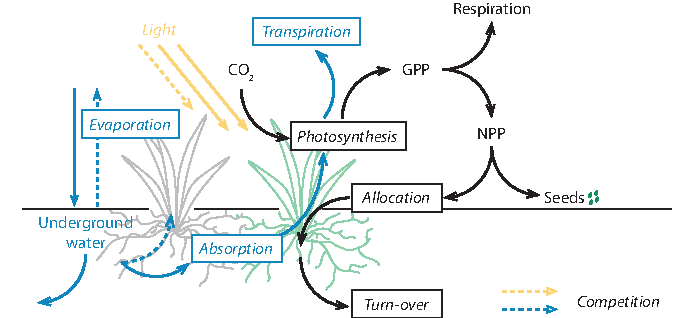
\includegraphics[width = 1\linewidth]{./1_Introduction/graphics/model_cycles.pdf}
\caption{Model overview. \textcolor{myBlue}{Water} and \textbf{carbon} cycles are represented. Processes are represented framed and in \textit{italic} by contrast with pools that are not framed and in regular fontface. Dashed arrows indicate loss of resource (for the \textcolor{myGreen}{focal plant}) due to competition.}\label{fig:overview}
\end{figure}


\subsection{State variables}

\paragraph{Scales}
In mountain grasslands individuals (tillers) generally do not grow big and interact only with close neighbours and form little patches. And thus it is possible to represent a rich community at a fairly small scale ($\approx$ dm or m), but the spatial resolution should be relatively fine ($\approx$ cm) to capture inter-individual interactions. Because the model is intended to explore climate change impact on mountain grasslands, it can run on multiple growth seasons separated by snow-covered periods, but must also integrate the intra-seasonal variations at daily scale. Mountain weather (mostly temperature) is known for its large hourly variations, it would, however, require too much computational power to consider such variations. In addition to this argument, we believe that even though they imply physiological flexibility and specific strategies for plants experiencing these conditions, they will not have a huge impact on overall community dynamics changes caused by the climate change. That why hourly variations will not be considered and physiological processes are estimated at the daily timescale.

\paragraph{Plants} The plants are described in the model by state variables described in table \ref{table:state_var_plant}. The best way to understand how plant are represented is to imagine two homogeneous cylinders on top of each other, the shoot cylinder varying in radius and height representing the light acquisition (and shading) zone, and the root cylinder varying only in diameter (because of shallow soil in mountain ecosystems) representing the water acquisition zone. These cylinders are centred on cells of the torus simulation plan.\\
\begin{marginfigure}
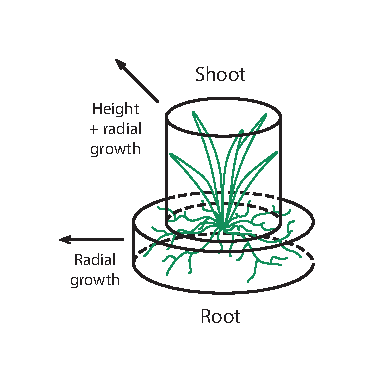
\includegraphics{./Figures/plant_geometry_m.pdf}
\caption{Plant geometry and growth axis.}
\end{marginfigure}
\indent In addition to classic variables (age, position, height, diameter, shoot and root biomasses) the plants are described by traits, that can be species-specific or non-specific, others are variable (SLA, SRL) and depend on particular traits that are unique to this model: the \textbf{ratio between active tissue and structural tissue} (in shoot and root) (variables $\frac{act}{str}_{ag}$ and $\frac{act}{str}_{bg}$ in table \ref{table:state_var_plant}). This couple of traits come from the evidence that numerous trade-off observed in leaves can be explained (at least partially) by this allocation trade-off between active tissue producing organic matter, but increasing respiration, and structural tissue that increase tissue lifespan.

%TAble of plant state variables
\begin{table2*}
\caption{State variables of individual plants} 
\label{table:state_var_plant}
%\begin{center}%
\begin{tabular}{l|l|c}
Variable & Description & Unit \\ 
\hline 
x & x position on the grid & cells \\
y & y position on the grid & cells \\
age & age & days \\
sp & species & - \\
$BM_{ag}$ & above-ground biomass & g \\
$BM_{ag_sen}$ & senescent above-ground biomass & g \\
$SLA_{sen}$ & senescent above-ground biomass & $cm^{2}.g^{-1}$ \\
$BM_{bg}$ & below-ground biomass & g \\
stem & stem biomass & g \\
$\frac{act}{str}_{ag}$ & above-ground active on structural biomass ratio & g/g \\
$\frac{act}{str}_{bg}$ & below-ground active on structural biomass ratio & g/g \\
h & height & cm \\
r & shoot radius & cm \\
r\_r & root radius & cm \\ 
$light_{exp}$ & above-ground potential resource availability & gH2O.leaf area\\
$water_{exp}$ & below-ground potential resource availability & gH2O.root area\\
\end{tabular} 
%\end{center}
\vspace*{0.5cm}
\end{table2*}

%little scheme to show what it looks like

\paragraph{Species} Plants are characterised by state variables that describe them individually, but they also share common characteristics with individuals of the same group, (we will refer as \textit{species} to talk about this group in the rest of the document even though it could be a group at another scale (i.e. population, clones). These species are the groups present in the meta-population and that can invade the simulated ecosystem. There are described by multiple traits characterising the strategy of the species (table \ref{table:state_var_species}).


%TAble of plant state variables
\begin{table2*}
\caption{Species traits}
\label{table:state_var_species}
\begin{center}
\begin{tabular}{l|c|c|l}
Trait & Range (close range) & unit & trade-off or strategy\\
\hline 
seed mass & (0.00001 - 0.001) & g & seed ouput vs seedling productivity\\
maturity & - & green biomass & flowering time vs reproduction potential\\
fract\_dev & 0-1 (0.05-0.6) & - & blooming vs persistence\\
fract\_rep & 0-1 (0-1) & - & reproduction vs persistence\\
geometric constant ($k_{g}$) & (0.1 - 20) & - & competition sensitivity vs self-shading\\
plasticity stability & 0-1  (0.8-1) & - & genetic information vs experience\\
initial water resource & (0.001 - 0.05) & $gH_{2}O.cm^{-2}$ & water resource niche\\
initial light resource & (0.001 - 0.05) & $gH_{2}O.cm^{-2}$ & light (in $H_{2}$ equivalent) resource niche\\
$\frac{act}{str}_{ag,d}$ & (0.03 - 0.3) & $g.g^{-1}$ & active vs structural tissue\\
$\frac{act}{str}_{gg,d}$ & (0.03 - 0.3) & $g.g^{-1}$ & active vs structural tissue\\
mean temp. & (0 - 5) & \celsius & early vs late germination\\
germination rate & 0-1 (0.5 - 1) & - & good season bet-hedging\\
thickness & 	(0.012 - 0.05) & cm & WUE vs light efficiency (not in this version)\\
\end{tabular} 
\end{center}
%\vspace*{0.5cm}
\end{table2*}
%table of species traits. trait, range, distribution, trade-off or strategy associated.

\paragraph{Seed-bank} The seed-bank is the transition state between the different seasons. Individuals may persist thanks to stored resources, but they can also reproduce by the production of new individuals. A lot of grasses use clonal reproduction, in addition, or replacement of sexual reproduction. This type of reproduction is characterised by a persistent link between the newly produced individuals and the parent one that allows the two to communicate and exchange resources. Such dynamics are complex and costly to represent as the link between ramets must be stored and strategies defined for the resource distribution (see Oborny 2012) for more details on clonal growth modelling). To avoid too much complexity, it is possible to approximate the representation of clones to big seeds with little dispersion around the parent plant\footnote{This would take advantage of dispersion kernels. Not implemented in the current version. Dispersion is uniformly random within the simulation plan}. For this reason, reproduction mechanism is reduced to sexual reproduction mechanism with the production of "seeds". Seeds are stored in the seed-bank and only defined by their species and positions. 

\paragraph{Soil}
\begin{marginfigure}
\includegraphics{./Figures/soil_section_m.pdf}
\caption{Soil section.}
\end{marginfigure}
The soil is an important aspect of the model as it drives (with the precipitations) the water competition between individuals. It is however limited, as in numerous vegetation models, to a grid characterised by its capacity to retain water, and its depth. Only the first component (water retention capacity) is spatially variable and is described by the critical water content (minimum soil water content), the saturation water content (maximum water content, the water non absorbed leaves the system we assume the same root depth for all species), and the current water content (temporally variable, depending on competition, precipitation and evaporation, between the critical and the saturation water content) only dynamic variable among the three.

%table of soil state variables

\subsection{Process overview and scheduling}

As mentioned the model runs at a daily step to capture individual responses to conditions and over multiple seasons to capture long temporal dynamics. Some processes occur (or are evaluated) at the daily time-step, some at the season time-step. The following ordered list presents the different processes and the scheduling over days and season of one simulation.\\
\indent One season can be divided into the following parts:
\begin{marginfigure}
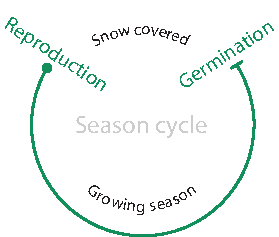
\includegraphics{./Figures/season_cycle_m.pdf}
\caption{Seasons cycle in \model.}
\end{marginfigure}
\begin{itemize}
\setlength\itemsep{0em}
\item \textit{germination}: marks the beginning of the season when the ground is no more snow-covered;
\item \textit{growing season}: consists in daily processes like competition, production of organic matter (OM), allocation, and death lottery;
\item \textit{reproduction-invasion-persistence}: marks the end of the season when the first persistent snow-fall occurs. OM invested in reproductive tissues turns into seeds that are sampled to create the seed-bank. Seeds from the meta-population may integrate the seed-bank. Persistent perennial loose most of their biomass but storage (and eventually stem) and regrow from stored organic mass at the beginning of the following season.
\end{itemize}

The \textit{growing season} part consists in all processes evaluated every day of the growing season. These processes are:
\begin{marginfigure}
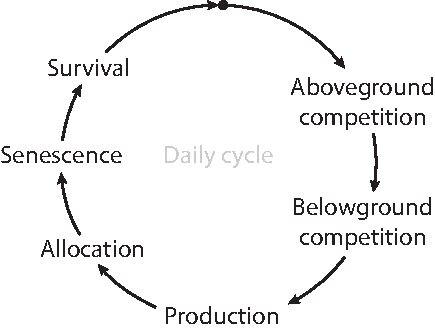
\includegraphics{./Figures/daily_cycle_t.pdf}
\caption{Processes in order during the daily cycle.}
\end{marginfigure}
\begin{itemize}
\setlength\itemsep{0em}
%\item \textit{resistance allocation}: the stored OM (in seeds or in storage tissues) are either invested in resistance molecules or in development;
%\item \textit{freezing}: frost damage on plants;
\item \textit{light competition}: the individual potential photosynthetic activity is computed based on average daily light and shoot properties;
\item \textit{water competition}: evaporation and the individual water update (and potential water uptake) are computed based on potential transpiration, water availability and potential evaporation;
\item \textit{production}: respiration and production are computed to give the net productivity in OM;
\item \textit{senescence}: based on lifespan a part of tissue is no longer active.
\item \textit{death}: death of individuals based on their age and their desiccation stage (number of consecutive days with negative growth).
\item \textit{allocation}: allocation of produced OM to the different carbon pools of the plant.
\textcolor{Gray}{\item \textit{grazing/cutting}: (optional) grazing or cutting of plants to a certain height. The grazing can be selective.}\footnote{remarks in \textcolor{Gray}{grey} are features or components implemented in the model but not used and-or calibrated.}
\end{itemize}


\section{Design concepts}

\subsection{Design concepts}
This part clarifies the rules that drive the dynamics of the model.

\paragraph{Emergence} 
The purpose of the model is to understand the rules that drive the community responses. We tried making the community dynamics emerge from the underlying processes of plant growth, resource use, and reproduction. That means that population dynamics are at least partially emergent from the surviving and reproducing individuals.
\textit{Partially} emergent because it depends on the invasion rules applied to the system. The traits and biomass distribution that describe the community are completely emergent from the individual traits exposed by the individuals and their relative biomass and abundance.
\begin{marginfigure}
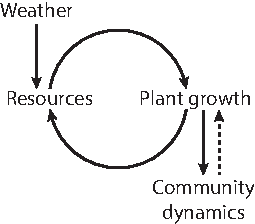
\includegraphics{./Figures/emergence.pdf}
\caption{Population dynamics emerging from plant growth and weather.}
\end{marginfigure}

\paragraph{Adaptation} Plants have in theory many options to adjust their phenotype and increase their fitness in response to changes in environmental conditions (resource availability, temperature, ...). High diversity of mountain grasslands suggests that multiple strategies coexist and that individuals do not change to converge toward a unique strategy. These strategies are set up at the species level by the species-specific traits (see table \ref{table:state_var_species}). Therefore, individuals may only adapt morphological traits but not strategic traits (unless there is an epigenetic mechanism added). These morphological traits are the relative biomass of shoot and root, the relative proportion of active and structural tissues in each leaf, and roots (controlling respectively the SLA and SRL and the overall resource acquisition cost)\footnote{and optionally the proportion of stored OM dedicated to frost resistance and not to growth}. Geometry traits (distribution of leaves and roots within space) are not considered plastic as grasses have far less control over their geometry than forbs or trees. Root distribution plasticity has been shown to greatly improve the individual and community productivity (Gemini article), but to keep the model (and implementation) simple we will ignore root distribution plasticity and foraging strategies to focus on allocation problems instead of spatial distribution questions. Shallow soils and relative small rooting zone are also arguments to ignore spatial distribution plasticity for roots.

\paragraph{Fitness}
\begin{marginfigure}
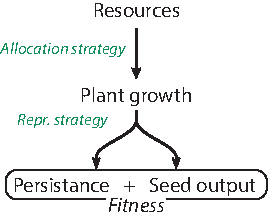
\includegraphics{./Figures/fitness.pdf}
\caption{Fitness emerges from the plant growth and the plant reproductive strategy.}
\begin{footnotesize}
The plant growth is the result of the interaction of the resource levels, the plant strategy, and the competitors.
\end{footnotesize}
\end{marginfigure}
In the model, the realised fitness can be estimated as the capacity of plants to maintain themselves or their descendants through time. It emerges from the productivity, allocation to storage or reproductive carbon pools, and survival. Assessing fitness as the average number of persistent individuals is, however, a bit hazardous in simulations limited in time and to a relatively small spatial scale. Plus, plants cannot easily make a prediction of such variable to adjust their phenotype. They need a proxy function for fitness that integrates measures of external conditions to evaluate the best strategy to develop. As said above, this strategy should be a composite between the species strategy and individual adjustment specific to the individual experience of the environment. Plant fitness is estimated by individual plant thanks to a gain function integrating current phenotype, species strategy, and projection of future conditions. This gain function can take multiple forms and be more or less constraint. In the context of the model, the function should include a measure of productivity that relies on the principle of functional equilibrium - that is the allocation of organic matter to maintain the balance between the shoot activity (transpiration) and root activity (water uptake). This equilibrium can be achieved by changes in shoot:root ratio only, or also changes in active over structural tissues ratio. Further details about the gain function are discussed in the dedicated paragraphs (\ref{par:allocation}). A more complex form of functional equilibrium incorporating nutrients (like nitrogen) could be added to the framework of this model.

\paragraph{Prediction} Adaptation or plasticity mechanisms imply that agents have an insight of what will be the future. In \model we consider that plants have two main sources of information. The first source of information is the genetic information. Indeed, the evolutionary process of genotype selection has led to the selection of genotypes adapted to the local conditions. This selection relationship can be seen as a link between environmental conditions and genetic information. Because plants cannot fully predict future environmental conditions, they grow following (at least partially) the plan contained in genetic information that match conditions where previous generations grew in.  This is an internal \textit{a priori} information about the external conditions. If the conditions where the seed grows change from the conditions its genotype has been selected for, the genetic information does not fit the environmental conditions is not sufficient enough to build a working phenotype. In this case, if the plant has a plasticity capacity, it can integrate the second source of information, in the form of the experienced conditions, to its "a priori" and forge a new estimation of what conditions will be. One question emerges to this idea is: how to create an image of future conditions and how to balance the genetic \textit{a priori} information with the experienced information? This balance can be described by a term of "reactivity" that describes the relative weight of genetic and experienced information. A reactive species will give a higher weight to experienced condition information, whereas a stable species will give a higher weight to genetic information.\\
\indent The way the two source of information are brought together and used to define the plant phenotype is at the core of plant strategy and is the main feature of the model \model.
\begin{figure}
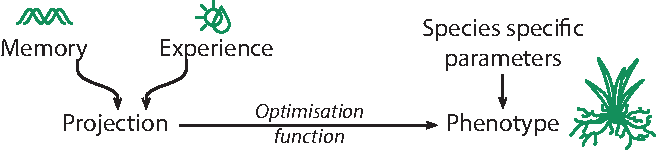
\includegraphics{./Figures/memory2phenotype_t.pdf}
\caption{Genetic and perceived information are both considered to determine the phenotype.}
\end{figure}
%\indent From that mechanism we can define two terms: the \textbf{climatic niche center} of a species is the \textit{a priori} information on climatic conditions, and the \textbf{plastic capacity} of a species is both its reactivity and its capacity to overcome the plasticity cost and invest in required tissues.
%Individuals do not estimate directly their fitness. They have however a way of estimating how well they perform depending on the level of resources they estimate. This measure is essential in plasticity mechanism as it drives plasticity. This measure is dependent on the plasticity mechanism chosen. Indeed plasticity can be approached in different ways that are discussed later, one mechanism consists in maintaining the \textit{functional equilibrium}, in this case, the fitness information is approached by the relative balance between above-and below-ground activities. The other mechanism is the \textit{optimisation}, that implies a more complex estimation of productivity, respiration, tissue turn-over and death changes and gives a more detailed approximation of individual fitness.
%\paragraph{Prediction and adaptation} As explained above, the "incomplete fitness proxies" used in the plasticity mechanisms require estimation of above- and below-ground activities, based on their trait values (SLA and SRL) and on an estimation of future external conditions (temperature, water availability and light availability). The originality of our approach is to make this estimation depending on both species-specific parameters and individual experience. The conditions are estimated as the weighted mean between the species-specific genetic \textit{a priori} on resource availability and the potential resource availability normalized over exchange area. This makes the estimation by one individual depending both on the species-specific "environmental niche" and the competition effects on resources. Moreover, this mechanism, because it includes relative weight to the two sources of information, allow multiple strategies for the estimation of external conditions and so on how to cope with resource levels variation.
%
%\paragraph{Adaptation} Adaptation is central in the model as we believe it explains a lot of intra-specific variability in mountain grassland ecosystems (cite Albert and others)
\section{Details}

Further details on daily mechanisms are described in the following paragraphs.


\begin{marginfigure}
%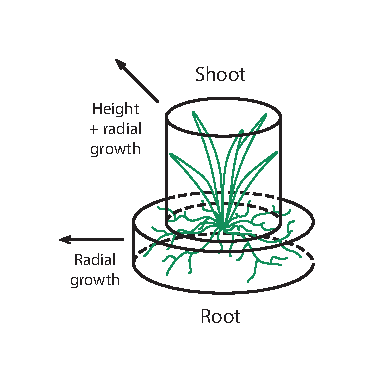
\includegraphics{./Figures/plant_geometry_m.pdf}
\caption{Overview of the model inputs and outputs.}
\end{marginfigure}

\subsection{Initialisation}
The model doesn't need particular initialisation if the state of the community species pool, the seedbank, and the soil are given as inputs. Otherwise, a set of \textit{E(n/s)} individuals are created from a set of \textit{s} species (randomly generated if not given) and randomly positioned on the soil grid, where \textit{s} and \textit{n} are respectively the number of species and the approximate number of individuals within the grid. Soil grid is also randomly generated within default ranges for critical and saturation water contents then slightly smooth, and homogeneously filled ($filling = \frac{w_{cont} - w_{crit}}{w_{sat} - w_{crit}}$).
 
\subsection{Inputs}
\model needs system state information (individuals, species, seed-bank and soil) and climate data. If the state of the system is not completely given, then the complete state is generated in the initialisation. The daily climate data at must contain the following fields:
\begin{itemize}
\setlength\itemsep{0em}
\item \textit{date};
\item \textit{radiance}, in $Watt.m^{2}$;
\item \textit{precipitation}, in mm;
\item \textit{mean temperature}, in K;
\item \textit{mean day temperature}, in K;
\item \textit{min temperature}, in K;
\item \textit{max temperature}, in K;
\item \textit{relative humidity} in \%;
\end{itemize}
Vapour pressure deficit is then computed from temperature and relative humidity.\\
\indent The climate data must explicitly differentiate the seasons (delimited by the first day of the year without snow and by the first day of the second semester with snow).

\subsection{Submodels}\label{subsection:submodels}

\paragraph{Germination} Individuals from the seed-bank randomly germinate according to their species-specific germination rate. Germination consist of investing a percentage ($mob$ parameter) of the seed mass into shoot and root biomass according to default traits. This is coupled with a round of random seed death following uniform law of parameter $seed_{surv}$. Living non germinating seeds stay in the seed-bank until the next season.\\
%
%\vspace{0.5em}
%\paragraph{Freezing resistance allocation} Resistance mechanisms are important for plants to invade harsh environments with perturbations such as grazing of frost events. Investment in free organic compounds is shown to provide resistance to frost. The concentration of such compounds is time variable and closely related to temperature. Other mechanisms morphological, structural, physiological can also play a role in frost resistance. For the sake of simplicity we will limit this aspect to the investment in circulating agents. Moreover, this aspect is crucial, indeed  because the frost risk is high at the beginning of the season, the choice of investing in resistance molecules instead of growing tissues is a strategy choice. Species can then be differentiated on a earlier growing/high frost risk - late growing/low frost risk axis, depending on their estimation of minimal temperature. Minimal temperature is estimated the same way other resources levels. Available stored biomass is invested in frost resistance is the estimated mean temperature is below 3\celsius .\\
%
% 
%\paragraph{Freezing} The freezing damages are calculated based on the concentration of organic matter dedicated to frost resistance is the plant. The LT50 (temperature at which 50\% of biomass is lost) is proportional to the concentration of resistance molecules compare to overall biomass. Daily leaf biomass lost due to frost is computed as follow:
%
%
%\begin{align}
%k_{frost} &= log(1/dam_{-1} - 1)/(-1 - LT_{50})\\
%dam &= \frac{1}{1 + e^{k_{frost}(T_{min} - LT_{50})}}
%\end{align}

\textbf{Daily processes}

\paragraph{Light competition}Light competition is central to all vegetation model as it constrains the photosynthetic activity and so plant growth. To avoid costly calculation of ray propagation we assume vertical homogeneous top radiation. Relief and orientation effects are taken into account in the computation of irradiance data.\\
Light competition sub-model allows calculation of individual potential photosynthesis activity and light at soil surface for evaporation calculation.\\
Competition for light is calculated independently for each pixel, potential photosynthetic activity is then aggregated at the individual level. Each pixel can be seen as a column of homogeneous layers containing at least one individual (top layer). For each layer, the light transmission is computed based on leaf density.


\begin{marginfigure}
\begin{tikzpicture}
\begin{axis}[marginplot,
legend style
={at={(1, 1.1)},
anchor=south east,
draw = none},
samples = 40,
%restrict y to domain=-300:700,
ylabel = $I_{h}$,
xlabel = $h$
%extra x ticks={0.618},
%extra x tick style={grid=major}
]

\addplot[black][domain = 0:10 ] {120 * exp(-1*x)};
%\addplot[gray][domain = 0:1 ] {(1/(0.022 * 1)) * ((1/0.05 - 1)*x) - %(7*exp(7*x) + 0.03)};
%\legend{$I_{h}$}
\end{axis}
\end{tikzpicture}
\label{fig:derivaives}
\caption{Net gain function and its first derivative.} Looks like there is some kind of mismatch here.
\end{marginfigure}

\begin{equation}\label{eq:Ih}
I(h) =  I_{0} e^{-LAI(h)}
\end{equation}

where $LAI(h)$ is the cumulative LAI at the bottom of layer \textit{l} (between $h$ and $h+\Delta_{h}$) defined as the homogeneous layer delimited by the top of consecutive individuals in the same pixel. The LAI is calculated like this:
\begin{equation}\label{eq:LAI}
LAI(h) = LAI(h+\Delta_{h}) +   \Delta_{h} . pix\_width^{2} \sum_{i\ in\ l}d_{i}.coverage_{i, p}
\end{equation}
where $d_{i}$ is the individual leaf area density corrected by the coverage ($0< coverage =< 1$) of the pixel $p$ by the plant $i$, $\Delta_{h} = (h_{l} - h_{l-1})$ is the height of the layer $l$.\\
Following Thornley and Johnson, the potential photosynthetic leaf activity is calculated as:


\begin{marginfigure}
\begin{tikzpicture}
\begin{axis}[marginplot,
legend style
={at={(1, 1.1)},
anchor=south east,
draw = none},
samples = 1000,
%restrict y to domain=-300:700,
xlabel = $I (W.cm^{2})$,
ylabel = $P_{leaf} (gCO_{2}.cm^{-2}s^{-1}) check that$
%extra x ticks={0.618},
%extra x tick style={grid=major}
]

\addplot[black][domain = 0:0.04 ] {(\paralpha * x * \parPmax ) /(\paralpha * x + \parPmax ) };
\legend{}
\end{axis}
\end{tikzpicture}
\label{fig:derivaives}
\caption{Photosynthetic saturation function}
\end{marginfigure}

\begin{equation}\label{eq:Pleaf}
P_{leaf}(h) = \frac{\alpha. I_{leaf}(h).P_{max}}{\alpha I_{leaf}(h)+P_{max}}
\end{equation}
where $I_{leaf}(h)$ is the light absorbed by the leaf at height $h$, $\alpha$ the initial slope of the light response curve and $Pm_{i}$ the maximum photosynthetic rate per unit of area and unit of time.
% where $I_{leaf}$ is the light absorbed by the leaf and the photosynthetic potential rate $Pm_{i}$ is linearly related to active biomass per leaf area as follow:
%\begin{equation}
%Pm_{i} = min(P_{slope} \frac{Leaf_{Act_{i}}}{Area_{i}}, P_{max})
%\end{equation}
$I_{leaf}$ is the radiance at the leaf surface, derived by correcting the radiance at the top of the layer following the equation used in Taubert with the extinction and transmission coefficients $k$ and $m$:

\begin{equation}
I{leaf}(h) = \frac{k}{1-m}I(h)
\end{equation}

The equation \eqref{eq:Pleaf} can be integrated over the leaf surface by mixing it with equations \eqref{eq:Ih} and \eqref{eq:LAI} to give the total potential photosynthesis for layer $l$ in pixel $p$:
\begin{equation}\label{Ppixlay}
P_{leaf}(p,l) = d_{i}.coverage_{i, p}.\Delta_{h}(l)\int_{h_{bottom}}^{h_{top}}P_{leaf}(h)
\end{equation}
%
%\begin{equation}
%P_{leaf}(l) = \int_{h_{l-1}}^{h_{l}}P_{leaf}.dLeaf = Leaf_{area}\left[- Pm_{leaf}.log(|m.Pm_{leaf} - Pm_{leaf} - \alpha.I_{h(leaf)}|)\right]_{h_{l}}^{h_{l-1}}
%\end{equation}

the total leaf potential photosynthesis is then calculated as follow:
\begin{equation}\label{eq:PS_pot}
PS_{pot} = \sum_{p\ in\ shoot}\sum_{l\ in\ pixel}P_{leaf}(p,l)
\end{equation}
\indent Potential photosynthesis must then be converted to potential transpiration to define the water demand. The conversion from photosynthesis to transpiration is done by dividing the potential photosynthesis by the water use efficiency ($WUE$). The potential activity of leaves are also dependent on the regulation of stomata so the transpiration can be written:
\begin{equation}
transp = \frac{PS_{pot} . g_{red}}{WUE}
\end{equation}

\textcolor{Gray}{\paragraph{Stomatal regulation} Photosynthesis depends on gazes exchanges at the leaf surface. These fluxes result from relative concentration in carbon dioxide and water, and from the stomatal conductance. Stomatal conductance is reduced and limits productivity when vapour pressure deficit is too high \sidenote{$g_{red}$ is set to 1 for current version to avoid potential problems between allocation and regulation}. A linear relationship describe this relationship:
\begin{equation}
g_{red} = 1+ VPD_{g\_red}
\end{equation}}

\paragraph{Evaporation} Potential evaporation is calculated for each pixel depending on the light at soil surface:

\begin{marginfigure}
\begin{tikzpicture}
\begin{axis}[marginplot,
legend style
={at={(1, 1.1)},
anchor=south east,
draw = none},
samples = 1000,
%restrict y to domain=-300:700,
ylabel = $\beta$,
xlabel = $\theta$,
extra x ticks={0.8},
extra x tick style={grid=major}
]

\addplot[black][domain = 0:0.8 ] {(1/4) * (1-cos(deg(x/0.8 * pi)))^2};
\addplot[black][domain = 0.8:1 ] {1};
%\legend{$I_{h}$}
\end{axis}
\end{tikzpicture}
\label{fig:derivaives}
\caption{Evaporation  limitation function.}
\end{marginfigure}

\begin{align}
 \beta &= 0.25 * (1 - cos(\frac{\theta}{\theta_{sat}} * \pi))^{2} & if water_{cont} \le water_{sat}\\
 \beta &= 1 & otherwise\\
 PET &= 0.0023. \sqrt{(T_{max} - T_{min})} * (T_{mean} + 17.8)\\
 evap &= PET . \beta . I_{surface} . daylength
\end{align}

\paragraph{Water competition} Water competition is also computed at the pixel level. To determine the water uptake, first the individual water demand is computed as the minimum between the transpiration and the potential water uptake. Transpiration demand per pixel is easily calculated by dividing the total potential transpiration by the volume in the pixel $V_{i,p}$ over the overall root volume $V_{i}$. Water potential uptake is the product of root area in the pixel and root water uptake rate reduced by the water availability reduction factor $U_{lim}$, leading to the water demand for individual $i$ in pixel $p$:
\begin{align}
transp_{i}(p) &= transp . \frac{V_{i,p}}{V_{i}}\\
Wpot_{i}(p) &= Root_{area}(p).U_{max}.U_{lim}\\
Wdem_{i}(p) &= min(transp_{i}(p), Wpot_{i}(p))\\
\end{align}
where, the limitation function $U_{lim}$ is defined as in \parencite{reineking_environmental_2006}:

\begin{marginfigure}[-40pt]
\begin{tikzpicture}
\begin{axis}[marginplot,
legend style
={at={(1, 1.1)},
anchor=south east,
draw = none},
samples = 100,
%restrict y to domain=-300:700,
xlabel = $\theta$,
ylabel = $U_{lim}$
%extra x ticks={0.618},
%extra x tick style={grid=major}
]

\addplot[black][domain = 0.21:0.99 ] {exp(\parbetazero * (1/(1-0.2) - 1/(x-0.2))) };
%\legend{Water limitation}
\end{axis}
\end{tikzpicture}
\label{fig:derivaives}
\caption{Water uptake limitation response function to soil saturation}
\end{marginfigure}

\begin{align}
U_{lim} &= exp\left(\beta_{\theta} \left( \frac{1}{\theta_{s} - \theta_{crit}} - \frac{1}{\theta - \theta_{crit}}\right)\right) & if \theta < \theta_{crit}\\
 &= 0 & otherwise
\end{align}

%Where $U_{i}$ is related to the maximum water uptake $U_{max}$ and to the the $\frac{Root_{Act_{i}}}{Area_{i}}$ as in equation \eqref{eq:Pleaf}.\\
The total water demand per pixel is then the sum of all individual water demand of the pixel and potential evaporation. If the total water demand exceeds the total water availability ($W_{av}$ product of water content and soil volume in the pixel) then the available water is distributed proportionally to the individual demand.\\
\begin{equation}\label{eq:water_uptake}
Wup_{i} = Wdem_{i} . \frac{Wdem_{total}}{min(Wdem_{total}, W_{av})}
\end{equation}


\indent The potential water uptake ($Wpup$), non limited by the transpiration is calculated the same way but considering $Wdem_{i} = Wpot_{i}$ in equation (\ref{eq:water_uptake}).\\
\indent Because the water competition is computed at the pixel level, there is no compensation between two pixels containing respectively not enough and too much water.\\
\indent No radial flow of water between pixel is implemented in the model. This simplification leads inevitably to edge effects, but allows simpler implementation and is partially covered by the effect of the pixel size. Indeed, increasing pixel size would have similar effect in the pixels at the border of the rooting zone than radial flow because it would increase the potential water pool plant has access to.\\

\indent Once potential and realised transpiration and water uptake are computed, 
plant productivity can be calculated.


\paragraph{Production, and respiration} Following previous vegetation models, the respiration is decomposed in growth respiration and maintenance respiration. The first is function of trait values, biomass and temperature:
\begin{equation}
R_{m} = \left(R_{act}.\left(Act_{ag} + Act_{bg}\right)\right) . daylength . T_{effect}
\end{equation}
where $R_{act}$ is the respiration rate of active tissues, and $Act_{ag}$ and $Act_{bg}$ are the active biomass pools in shoot and root.\\
\indent Net Primary production (in $CO_{2}$ equivalent) can then be calculated the difference of GPP and respiration, then converted in OM production thanks to tissue carbon content (under the assumption of fixed carbon content for leaf and roots between species):
 \begin{align}
 NPP_{carbon} &= (1- R_{g}) . (WUE . min(w_up, trans_p) - R_{m}) - BM_{total} * Pl_cost\\
 NPP_{OM} &= NPP_{carbon} . (12/44) / TCC
\end{align} 
Here $R_{g}$ is a fixed parameter but is set to $0$ if the difference between gross productivity ($GPP = WUE . min(w_up, trans_p) - R_{m}$) and maintenance respiration is negative. $Pl_{cost}$ is the plasticity cost as calculated in the dedicated paragraph below.

\paragraph{Temperature effect} Temperature has a effect of plant activity, this effect can be modelled by a bell shape function around an optimum value of 20 \celsius . See Lohier for details.


\paragraph{Condition estimation} The projection of environmental conditions is central in any implementaion of phenotype plasticity. Differences between the current perception of environment and the projections lead to adjustment of phenotype to increase fitness. In the model \model this projection results from hte averaging of two key concept: memory and perception. The latter is relatively simple to understand and corresponds to the perceived resource availability computed as the mean potential exchange rate per unit of area (total leaf or root area) and per hour(the hourly measure is used instead of daily measure to simulate the ability of plant to perceive the photoperiod. This is an easy way of taking into account one aspect of seasonality without complicating the model. However, it also reduce the range of memory and its impact to determine the phenotype, as an additional information would be needed to define the optimum phenotype: the day length).:
\begin{align}
light_{exp} &= \frac{transp}{exhange area_{ag}}\\
water_{exp} &= \frac{Wpup}{exchange area_{bg}}\\
\end{align}
The former is related to the species (or group) history and result from processes of selection and acclimation. It is the default projection of resource availability when the plant is not plastic. 
\begin{align}
light_{est}(t+1) &= (1 - \tau).light_{exp}(t) + \tau . light_{memory} . daylenght(t+1)\\
water_{est}(t+1) &= (1 - \tau).water_{exp}(t) + \tau . water_{memory} . daylenght(t+1)
\end{align}
\indent Because these are supposed to be expected conditions for the future, other formulation can be used instead of an average that is likely to introduce a lag in estimations. For example the following equation allow for a more stable projection that better fits the slower process of plant physiology adjustments:
\begin{align}\label{eq:projection_alt}
light_{est}(t+1) &= ((1 - \tau_{react}).light_{exp}(t) + \tau_{react} . light_{est}(t))((1 - \tau_{amp}) + \tau_{amp} . light_{memory}) . daylenght(t+1)
\end{align}
with $\tau_{amp}$ and $\tau_{react}$ being respectively amplitude and reactivity where only $\tau_{amp}$ is used in the first equation. Such solution could limit sensitivity and phenotypic instability. IN addition, such formulation would also better capture the accumulation of stress signals and would lead to a softer and more stable phenotypic shift.\\
\indent The estimation of external conditions as expressed here is then used to select the best allocation scheme during the allocation process. Limited here to levels of two resources (light and water), this estimation equation could be extended to other mechanisms such as herbivory risk, frost risk, humidity impact on water pressure deficit.\\

\paragraph{Allocation} \label{par:allocation}
Allocation is primordial in plant development and ontogeny. The following paragraph detail the implementation of the plastic allocation in \model.\\

\textbf{Maturity:} For most of plants the development cycle is divided in two phases of different durations: the vegetative phase when plant growths organs to gather resources and product OM, and the reproductive phase when plant take advantage of these organs to accumulate carbon and invest them in reproduction mechanisms. Plants are considered mature (they switch from vegetative to reproductive phase) in \model when the phenologic variable has reach a species specific threshold. The phenologic variable can be either the age, the height, the biomass, degree.days, in the current version total living biomass is used as trigger for reproductive phase.\\

\textbf{Allocation to supporting tissues:} Even-though grasses do not grow tall vegetative parts like trees, some grow vertically and they are exposed to stronger winds than most of forest. Therefore they need structural supports\sidenote{This supporting tissue mechanic is also needed to avoid exponential growth rate.}. Not all grasses grow stem, but they'll have stronger central vein in their leaves to structurally support the weight of leaves. In addition shoots and roots also need supporting tissues for water transport, for this reason the minimal mechanical support needed is calculated as a function of total living biomass:
\begin{equation}
support = \alpha . (BM_{ag} + BM_{bg})^\gamma
\end{equation}
where $\alpha$ and $\gamma$ are allometry coefficients.\\

\indent At each time step we must determine what fraction of new OM will be allocated to tissues growth while the remaining will support these need tissues. This leads to an optimisation problem numerically solved by the function \texttt{uniroot}.\\
%Despite the ambiguity in the name, there is a fundamental difference between structural tissues and supporting tissues: the former is part the individual organs and  
%\indent To avoid complex allocation optimisation problem, the allocation of supporting tissue is done before any other allocation. Is the support is not sufficient, no organic matter can be invested in vegetative development. The biomass the plant needs to invest in the stem is defined as:
%\begin{equation}
%\Delta_{stem} = max(support - (stem + Str_{ag}), 0)
%\end{equation}
%where $Str_{ag}$ is the structural biomass in shoot.\\
\begin{figure}
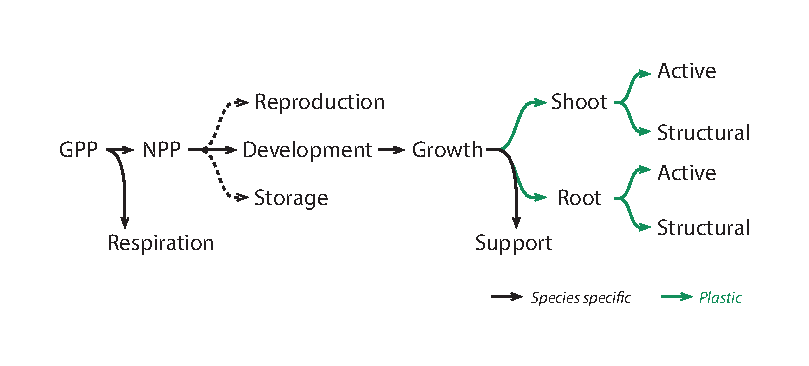
\includegraphics{./Figures/allocation_path_t.pdf}
\caption{Allocation of produced organic matter to different processes and pools.}
\end{figure}

\textbf{Allocation to organs:} Allocation of produced organic matter is central in vegetation as it shapes the plant and define the strength of the different organs. There are multiple ways to model the distribution of produced organic matter between the plant organs. We believe that such mechanism has great impact on individual development and response to external conditions, and so on community dynamics. To explore the role of this mechanism, multiple options are implemented. The different allocation algorithms are summarised in table \ref{table:alloc_algo}.\\
\indent There are two major components in the allocation algorithm:
\begin{itemize}
\item the objective function;
\item the plastic dimensions.
\end{itemize}
The \textit{objective function}: it is the function that give an fitness estimation or gain metrics for any given phenotype. This function is used to compute the optimum phenotype (phenotype at which the function is evaluated at the maximum value), or rank alternative phenotypes\sidenote{in this case, if not all possible phenotypes are tested, the solution might be only a local optimum. This is the case in \model.}. \\
The \textit{plastic dimensions}: they are the dimensions along which the individual can move. The space defined by these dimensions is the phenotypic space within which each individual plant can look for an alternative phenotype. They do not necessarily fully define a phenotype since some dimensions of the individual's phenotype can be fixed \sidenote{either by shared parameters of species specific ones.}. \\
\begin{figure}
\includegraphics{./Figures/strategy_space_algo.pdf}
\caption{Trajectories of a plant in the trait space depending on the plastic dimensions explored.}
\end{figure}
\indent The objective of this step of the model is to solve the objective function with the unknown variables being the plastic dimensions (RSR, SLA and SRL). In case of simple equations an analytical solution could be used to find an optimum \sidenote{under the condition that such optimum exists. The design of the model should ensure that.}. However, because the analytical solutions are already non trivial and the model is likely to evolve, a numeric solving method is adopted. \textbf{Need to detail the random algorithm.}\\
Also make a note on multiple optimum and the choice for a 'gradient descent" type of algorithm. Also sensitivity at eraly stages 

%TAble of plasticity mech
\begin{table*}
\caption{Allocation algorithms implemented in \model} 
\label{table:alloc_algo}
%\begin{center}%
\begin{tabular}{l|c|c c c}
Algorithm & Objective & variable RSR & variable SLA-SRL & stochastic \\ 
\hline 
No plasticty & $-$ & $\circ$ & $\circ$ & $\circ$ \\
Equilibrium & functional eq. & $\bullet$ & $\bullet$ & $\bullet$ \\
Eq-Fixed & functional eq. & $\bullet$ & $\circ$ & $\bullet$ \\
Optimisation & instantaneous gain & $\bullet$ & $\bullet$ & $\bullet$ \\
Optim-Fixed & instantaneous gain & $\bullet$ & $\circ$ & $\bullet$ \\
\end{tabular} 
%\end{center}
\vspace*{0.5cm}
\end{table*}

\textbf{No plasticity allocation:} this allocation is very similar to classic vegetation model where the biomass is allocated to the different carbon pools according to species specific parameters. But \model differs from other models by the order of the different steps of growth. In this model, the senescence comes between the allocation step and the resource competition-production steps \sidenote{see plastic allocation algorithm for explanation}. The partitioning coefficient are directly computed from species default trait to maintain the phenotype after senescence.

\textbf{Fixed trait allocation:} The fixed allocation supposes the allocation on OM to maintain trait values to fixed species specific values. The shoot:root ratio may however change to maintain functional equilibrium. The shoot root ratio is derived from the following equation of the functional equilibrium:
\begin{align}\label{eq:equilibrium}
SLA . BM_{ag} . light_{est} &= SRL . BM_{bg} . water_{est}\\
\frac{BM_{ab}}{BM_{bg}} &= \frac{SRL}{SLA} . \frac{water_{est}}{light_{est}}
\end{align}
where $light_{est}$ and $water_{est}$ are the estimated resource availabilities.
%
%\subparagraph{Plastic functional equilibrium} This allocation mechanism is also based on the functional equilibrium, however it incorporate changes in traits, that means that the proportion between active and structural tissues in an organ can change. This idea is supported by tha fact that plants change both their shoot:root and their trait values when conditions change. From a perspective with only one allocation dimension (shoot or root in "fixed trait allocation") with three dimensions (shoot or root, active or structural in shoot and in root tissues), the number of constraints must increase to find a unique solution. The functional equilibrium only is not sufficient to define the allocation scheme as multiple solutions satisfy this constraint. The solution is to chose among all possible allocation schemes the closest to the current allocation, the shortest path to functional equilibrium. This is done by minimising the 
% doesn't work for now

\textbf{Plastic trait allocation:} Another approach to allocation is to try to optimize phenotype based on a fitness proxy. This proxy can  be the sum of NPP, tissue turn-over loss and plasticity cost. But in a complex model like \model, plant performance is function of multiple aspects:\
\begin{itemize}
\item individual organ efficiency;
\item relative mass of each organ;
\item balance between organ water exchange activities.
\end{itemize}
And this could be extended to herbivory or frost risks. To take into account all these components, and take advantage of having all processes already made explicit by the implementation in the model, the daily processes of senescence and production are recalculated according to the \textbf{estimation of conditions} and the plant phenotype. This function is used to rank different alternative phenotypes (algorithm detailed below).

\textbf{Plastic trait equilibrium:} An alternative approach can be easily derived from the previous one and extend the principle of the first: the functional equilibrium with plastic traits. This approach consists in using the same algorithm as before but rank phenotypes with a function negatively correlated to the difference between estimated shoot and root activity. Such mechanism would nonetheless require the algorithm to look for close solutions within the allocation space to avoid convergence or drift from species strategy. Having non zero cost of plasticity in this approach should limit the drifting of the plant phenotype.

\textbf{Fixed trait optimisation:} This algorithm takes the idea of the optimisation algorithm but limits the plastic traits to the RSR ratio. If we can expect similar response than the fixed trait equilibrium if we suppose that the equilibrium is the main aspect of plant performance, global efficiency being considered in this case the result may vary.

\paragraph{Plastic algorithm}

Alternative phenotypes are computed from the actual phenotype and random uniform distribution of available organic matter to the main active and structural carbon pools of the plant.\sidenote{talk about the order senescence production, and the way exchange rates are computed.} ... This algorithm has the advantage of being relatively cheap compared to other optimization functions, however, its performances are variables and it is very sensitive to the number of samples used. As a consequence there is a trade-off between model stability and performance as a function of the number of samples (\textit{i.e.} alternative phenotypes) considered.
\begin{figure}
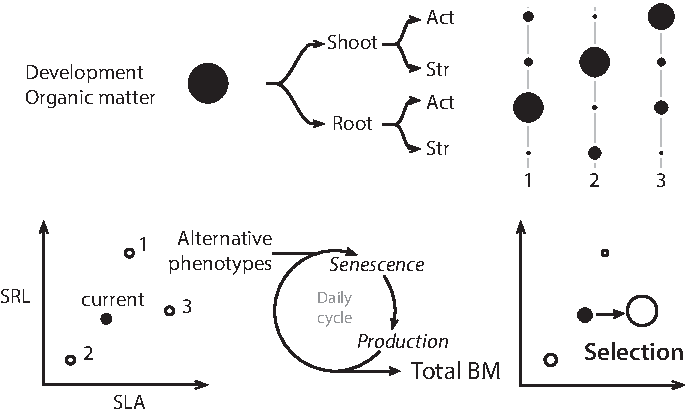
\includegraphics{./Figures/phenotype_ranking_t.pdf}
\caption{Algorithm for the evaluation and selection of randomly generated alternative phenotypes.}
\end{figure}

\paragraph{Plasticity cost}
The limits and costs of plasticity have long been discussed in the related literature. If \model is intended to be used to examine ecological costs and limits, it has to include physiological aspects of plasticity limits. There are two physiological processes involved in the mechanism of altering a phenotype based on changes in external conditions: sensing and signalling. 'Sensing' relates to the capacity of the individual to perceive environmental conditions. This is related to the capacity of the individual to perceive the environment and should, therefore, be considered constant over time. To take into account the cost of precise sensing, the first component of the plasticity cost is proportional to $\tau$.\\
The other component is related to the capacity of the plant to transmit this knowledge of conditions to change the development plan toward a new phenotype. This cost is proportional to the carbon-based distance (calculated as the difference between proportion of active tissues) between the default phenotype and the alternative (during allocation algorithm) or current phenotype.\sidenote{We could imagine cost based not on the default, but the previous phenotype, but it would have lead to large phenotypic shifting and convergence.}\\
Plasticity cost is the sum of both component and is proportional to the total biomass since most of the tissues should have the appropriated cell machinery and are affected b plasticity.
\begin{align}
pc_{maintenance} = (1 - tau) * pc_m \\
pc_{plasticity} = d_{traits} * pc_p
\end{align}
where $d_{traits}$ is the Euclidean distance between default phenotype and the alternative phenotype in the space defined by the proportion of active tissue for shoot and for roots.

\paragraph{Trait update}
Plasticity in trait suggests that trait values are modified in time. Because plants are described by single values (e.g. one SLA value for all leaves), this values must be updated after the plastic allocation. This values could be updated as the average of old tissue value weighted by old biomass and new tissue value weighted by the freshly produced biomass. This, however, would work only if active on structural tissues ratio linearly linked to others traits. This is not the case, it is then simpler to consider that organs have uniform active and structural distribution. This hypothesis suggests that whenever the allocation scheme change, old tissue reallocate their own biomass to follow the new scheme. Nevertheless, to avoid full plasticity allowed by this hypothesis, the changes in trait carbon pool sizes are limited by the produced biomass available for plant development.\\ollowing the following survival probabilities:


\indent From this, supposing homogeneous distribution of active and structural tissues within an organ allows to directly link the size of the carbon pools to average traits by the following relationships:
\begin{marginfigure}
\begin{tikzpicture}
\begin{axis}[marginplot,
legend style
={at={(1, 1.1)},
anchor=south east,
draw = none},
samples = 100,
%restrict y to domain=-300:700,
xlabel = $p_{act_{shoot}}$,
ylabel = $SLA$
%extra x ticks={0.618},
%extra x tick style={grid=major}
]

\addplot[black][domain = 0:1] {1/(\parth *  x * \parrhoas + \parth * (1 -  x) * \parrhoss * \parvts) };
%\legend{Water limitation}
\end{axis}
\end{tikzpicture}
\label{fig:SLA}
\caption{Specific Leaf Area as a function of the proportion in active tissues in shoot}
\end{marginfigure}

%  th_{a} &= \frac{\frac{act}{str}_{s} . th . \rho_{ss}}{\rho_{as} + \frac{act}{str}_{s} . \rho_{ss} }\\
%  s_{a} &= \frac{\frac{act}{str}_{r} . s_{root} . \rho_{sr} }{ \rho_{ar} + \frac{act}{str}_{r} . \rho_{sr}}\\
\begin{align}
  SLA &= \frac{1}{(th .  p_{act_{shoot}} . \rho_{as} + th . (1 -  p_{act_{shoot}}) . \rho_{ss} ) . V_{t}}\\
  SRL &= \frac{1}{(s_{r} .  p_{act_{shoot}} . \rho_{ar} + s_{r}.(1 -  p_{act_{shoot}}) . \rho_{sr}}
\end{align}


\paragraph{Senescence}

Senescence is the process of ageing of tissues. This process usually occurs at the scale of an individual organ (e.g. a leaf), however, \model does not consider organs independently because it would be complex and computationally expensive to follow multiple leaves and roots for all individuals. So the process is considered homogeneous over all tissues. To emulate the senescence process senescence is calculated from the tissues lifespan, giving :

\begin{marginfigure}
\begin{tikzpicture}
\begin{axis}[marginplot,
legend style
={at={(1, 1.1)},
anchor=south east,
draw = none},
samples = 500,
%restrict y to domain=0:1,
xlabel = $P_{act}$,
ylabel = $Lifespan (days)$
%extra x ticks={0.618},
%extra x tick style={grid=major}
]

\addplot[myGreen][domain = 0:0.99 ] {(\parlsszero * (1- x^\parlssone) ) };
\addplot[black][domain = 0:0.99 ] {(\parlsrzero * (1- x^\parlsrone) ) };
\legend{Aboveground, Belowground}
\end{axis}
\end{tikzpicture}
\label{fig:lifespan}
\caption{Lifespan of organs as a function of proportion of active tissues.}
\end{marginfigure}

\begin{align}
sen_{leaf} &= \frac{1}{LLS}\\
sen_{root} &= \frac{1}{RLS}
\end{align}

Because \model does not contain any mechanism preventing plant from growing only  active tissues\sidenote[][5pt]{it was intended to make the WUE negatively correlated to the amount of structural tissue per area.}, it is necessary for this cost function to make this strategy unreliable. The is then expressed as follow:

\begin{align}
LLS &= LSs_{s0} * (1- p_{act_{shoot}}^{LSs_{1}}) \\
RLS &= LSr_{s0} * (1- p_{act_{root}}^{LSr_{1}})
\end{align}


where $LLS$ and $RLS$ are respectively the leaf and the root lifespans calculated as negative log-linear relationships with the proportion of active tissue.\\
\indent Root senescent tissues disappear from the system. Information about senescent aboveground biomass is stored, but senescent biomass effect of light competition is ignored in this version because as it is implemented senescent tissues appear early in plant development and have large negative effect on light absorption.\\
\indent To the natural senescence and artificial cost of having only active tissue, an additional component can be added to the turn-over rate: the negative NPP. In case of negative NPP, the biomass will be taken from the already allocated following the shoot:root ratio. This can lead to a lower overall productivity (negative growth during unproductive periods) but also changes in the equilibrium if tissue have different efficiencies.\\

\paragraph{Death} Death is modelled as in Reineking \parencite{reineking_environmental_2006}. Age and desiccation (negative NPP) are the two reasons why a plant can die. The two death mechanism are simulated by independent random lotteries following the following survival probabilities:

\begin{marginfigure}[-10pt]
\begin{tikzpicture}
\begin{axis}[marginplot,
legend style
={at={(1, 1.1)},
anchor=south east,
draw = none},
samples = 100,
%restrict y to domain=-300:700,
xlabel = $age (days)$,
ylabel = $survival$
%extra x ticks={0.618},
%extra x tick style={grid=major}
]

\addplot[black][domain = 0:100] {exp(-((x/ \paralphaa)^\pargammaa- (max(x - 1, 0) / \paralphaa)^(\pargammaa)) ) };
%\legend{Water limitation}
\end{axis}
\end{tikzpicture}
\label{fig:derivaives}
\caption{Age related survival probability function}
\end{marginfigure}

\begin{align}
P_{d} &=  exp \left( - \left[\left(\frac{des}{\alpha_{d}}\right)^{\gamma_{d}} - \left(\frac{max(des - 1, 0)}{\alpha_{d}}\right)^{\gamma_{d}}\right]\right) & if NPP \le 0\\
&= 1 & otherwise\\
P_{a} &= exp \left( - \left[\left(\frac{age + 1}{\alpha_{a}}\right)^{\gamma_{a}} - \left(\frac{age}{\alpha_{a}}\right)^{\gamma_{a}}\right]\right)
\end{align}

State of dead individuals is store until the end of the season when seeds are stored in the seed bank. Seeds of dead individuals then join other seeds.

\paragraph{Reproduction \& persistence}
\textbf{Sexual \& clonal reproduction:} reproduction is handled at the end of the season. To limit the number of parameters reproduction is limited to the division of the invested biomass in reproduction by the species-specific seed biomass into a round number of seeds (the number of seed per plant could also be a differentiation axis). Clonal reproduction is not explicitly represented but can be mimic with bigger seeds and by adding a dispersion process around the parents. The seeds then are added to a potential seed-bank. This potential seed-bank is sampled, after eventual invasion, and merged with the existing seed-bank.\\
%\indent Control on the sampling process allows to model different type of ecosystems and test different hypothesises on invasions impact on community dynamics. The link between the community and the meta-community can also be explored through seed-bank control.\\
%\indent Three types of invasion/reproduction are currently implemented:
%\begin{itemize}
%\item closed environment reproduction: the seeds produced in the community return to the community, no invasion, the seed-bank size can be limited by a seed density limiting calculation explosions and simulating density mortality. Such mechanism should, in theory, lead to low diversity unless close equivalence between some species;
%\item constant reproduction in open environment: the seed-bank is generated at the meta-population levels, all species have the same biomass invested in reproductive pool independently from the local performance and seeds are randomly sampled. This mechanism stabilize greatly the system by does not allow to explore the meta-community dynamics and selection processes;
%\item productivity dependent reproduction in open environment: this mechanism is similar to the previous system but incorporates the productivity of the system by defining the seed input biomass as the total invested biomass in reproduction in the system at the end of the season. The system is stabilised but the overall productivity impacts the seed-bank dynamic.
%\end{itemize}

\textbf{Persistence} Some grasses are perennial and persist over the cold season. This is allowed in the model by investment in storage tissues instead of reproductive tissues.  At the end of the season, marked by the first snowfall, these plants (with non-null storage biomass) lose their living and supporting biomass, but will regrow from a large pool of store organic matter.

\textcolor{gray}{\paragraph{Grazing/cutting} Explore management effect on the community is one of the aims of the \model model. The management of mountain grassland will be explored only of the aspect of biomass removal, as productivity changes can be explored by changing the parameter values as the nutrients are not explicitly modelled. The management sub-model is not detailed here but it is based on the mapping of biomass and target trait (e.g. the fraction of structural biomass as a proxy for digestibility). Both cutting and grazing can be modelled but require management plan in the form of calendar of management operation and a cutting height or harvest objective.}\\

\section{Limitations and problems}

\subsection{Link to the real world and data}
The generalized framework introduced in \model allows to create a rich community in a high number of dimension strategy space, it, however, comes with downsides.\\
\indent One of the first problems is that some parameters (not explicitly detailed here) are hard to access (e.g. tissue density of active, or structural, tissue). It makes the calibration long as the incertitude for some parameters is very high. This is problematic when calibration is made difficult by a large execution time (see subsection below).\\
\indent Another issue with such model is that the high dimensionality of the species strategy space allows a lot of different strategies that are not viable. This could be overcome by selection mechanism over multiple plots, but again require a lot of simulation. Moreover, there are dependencies between viable strategies and parameter values that make it hard to restrict meta-community to viable species to set-up calibration runs.\\
\indent It is possible to extract summary statistics from the model output and compare them to information from collected data making calibration and community analysis easy. However going from the data to feed the model is harder, indeed without a great knowledge of a species it is hard to define its representation within the model framework. To do so would require the knowledge of the plasticity capacity to set the reactivity, anatomical traits to define default ratios of active over structural tissues, and climatic niche to define the \textit{a priori} estimation of external conditions. Without making a direct association with real species, it is possible and interesting to try to reproduce some strategies and explore their response to various conditions.

\subsection{Technical problems}

The model is implemented in \texttt{R} with some limiting function using \texttt{RCPP} to speed up the process. Simulations are fairly slow compare to theoretical \texttt{C++} equivalent code. The main problem is the choice of the data structure. Indeed agents are stored in data.frames that are often modified with the \verb|mutate| function, that makes the implementation much easier and the code readable, but slow down the execution due to constant condition checking on operations. This makes calibration routine methods almost impossible to use as they demand a very number of runs to be efficient.\\
\indent The slowness of the model also limit to simple algorithms for the research of favourable positions in the allocation space.
%\section{Model overview}
%\paragraph{pseudo-code and routine}
%\paragraph{allocation}
%mechanism and stochasticity\\
%5 types of allocation\\


%Take home message ####################################

%
%\subsection{Concepts}
%\paragraph{Memory} Genetic memory (see Sonia Sultan book for references). Selection and evolutionary processes.
%\paragraph{Equilibrium and efficiency}
%\paragraph{Optimum, strategy and memory} There might be optimum. But not easy to compute, especially when you consider more complex cost and interactions. Depend on different efficiencies and equilibrium... Also, you may want to avoid efficient by risky strategies (if you wrong, or if there is a quick shift). Need for strategic traits to drive allocation more than memory.\\
%Ok but what happen with optimisation allocation ? -> need the strategy to be tightly linked to memory. But that part has requirements: memory is a reliable source for strategy. Ultimately the resource availability is only one (ok, maybe two) dimension to phenotype optimisation. This strategy trait is necessary as other aspects of fitness are ignore (temperature implemented but not tested, grazzing vulnerability, frost damade, WUE, CO2 etc...) If you multiply mechanisms affecting the fitness you complexify the fitness landscape and allow for multiple strategies to be explored. Otherwise you must aartifically constraint. \\
%
%\indent \textbf{This is crucial to discuss this important aspect of strategic differenciation emerging for processes and how plant change strategy as the projection of environment evolves. Memory then plays more a role of sensitivity (with tau).}\\
%But for the moment the partial implementation of that through the artificial but meant to disappear default strategy is making analysis and assumptions difficult. Ok, but how do you treat it ? 
%
% equilibrium, resource use, resource availability, condition estimation
%\paragraph{Condition estimation}
%Important role of condition estimation. Perception mechanisms. (cost). Difference between plasticity and acclimation and epigenetics. 
%
%\subsection{Implementation}
%Why the use of a sampling method: complex effect of allocation and complex allocation system that is meant to be extended. Some results on the stability of phenotypes. How sampling method can drive the allocation.
%
%
%\section{Perturbations and resistances}
%
%\subsection{Climate}
%
%\subsection{Management}



%Take home message ####################################


%
%\subsection{comparison of different algorithms}
%full plasticity : freschet 2015 in poorter \& Ryser 2015
%the two sides of the performance/fitness: equilibrium and tissue efficiency\\
%age vs biomass.
%
%\section{Community dynamics parametrisation}
%Obj: demonstrate that the model is able to reproduce community dynamics (as it was designed for).\\
%Find parameters that allows coexistence (suggest plasticity should allow a diversity of strategy). SLA and height data. Phytosociology for 10m quadrats.

%
\chapter{Model properties and individual responses}
%%(Related to the notions cited above, like performance decomposition)
%Question I try to answer: (use of schematics ?)

The modelling framework developed in previous chapter offers multiple options to explore the effect of phenotypic plasticity on plant growth, and later plant community dynamics. Before investigating the effects of such mechanisms on complex systems dynamics, it is important to have a deep understanding of the model behaviour at individual level. As explained in introduction, the relationship between resource and individual plant growth is the base for plant interactions, abiotic filtering and coexistence mechanisms. This chapter of the document focuses on the calibration and exploration of the model for isolated individuals. The results of the simulation experiments exploring diverse aspect of resource-plant growth relationship will be interpreted at individual scales, but I will also attempt to extend conclusion to higher level mechanisms.

The first part of the chapter is dedicated to the parameter filtering process, the sensitivity analysis and basic model behaviour. Then follows the exploration of plant performance as a function of plant strategy and resources levels and dynamics.


% ##################################################################################
\section{Parametrisation and sensitivity analysis} \label{section:calibration}

Calibration, or \textemph{parametrisation}, is an essential step in the development of an agent-based model. ABMs are often characterised by multiple processes, and though parameters, at individual levels. The results of these processes (depending of parameter values) from numerous individuals combine to produce the group or community behaviour. Because there are interactions between the processes and between the agents, the overall behaviour of the group (often the subject of interest) is sensitive to these parameters. For the same reasons, an incredible variety of results could be produced with ABMs if the parameters where not chosen in order to produce sensible responses to simulated conditions. The aim of the calibration is to determine, from the \textit{a priori} knowledge of the processes and parameters, and the comparison with data, the best values for the model parameters. This step often goes along with a sensitivity analysis that determine the relative sensitivity of variables of interest to specific parameters.

Because of their nature, ABMs often model processes for which the parameters are either unknown, or hard to access (because at the individual scale). In such cases, advance calibration techniques like pattern oriented modelling\cite{grimm_pattern-oriented_2005, hartig} can be developed. However, such method require a high number of simulations and relatively precise simulation parameters. Because the implementation in R makes the model relatively slow, and because available datasets, despite being very interesting lack information on sensitive parameters, a less robust but less expensive approach is chosen: \textemph{parameter filtering} at the individual scale. The focus of the part of this work on the individual growth, and the will for more individual-centric approach also support this choice.

 For similar reasons of computational cost, the \textemph{sensitivity analysis} is  realised \textit{a posteriori} on calibration runs.

\subsection{Method}

\paragraph{Pot data}
Pot data consists in total biomass and root shoot ration (RSR) data of 11 species grown in pots by Peterson and Billings \cite{peterson_growth_1982}. This dataset has the advantages of being grass species grown in a described steady environment with two conditions of watering with measures of essential components of growth: biomass and RSR.

\paragraph{Pot simulation}
Simulated plant grow in square pots 9 cm wide and 12 cm deep. The soil is characterised by the following parameters: critical soil water content: $0.1 m^3.m^{-3}$, and saturation water content: $0.1 m^3.m^{-3}$. Simulation time of 111 days of 15 hours is divided between the growing phase of ... days, followed by the treatment phase when plant are water (soil saturation) either once a week or once a day. The light level and water influx are simulated with water event of ... mm and lighting of ... Watts per square meter.
Plants have default geometry parameters and reproduction is ignored and I assume plants do not stop their growth.

\paragraph{Parameter filtering process}
The whole filtering process has been implemented in \texttt{R}. Model parameters are sampled following the LHS method (from \texttt{lhs} package) within parameter ranges (described in table \ref{table:priors}) defined both thanks to the literature and constraints dictated by desired behaviours from the model. When necessary the sample is log transformed. Because of strong relationship between exchange rate parameters and cost of exchange area, exchanges rates parameters are expressed on a mass basis for sampling then transformed into an area basis for the model. To avoid extreme RSR ratios, the ratio between the mass based exchange rate parameters is limited between 0.1 and 10.

As explained in previous chapter, species specific parameters are requited to model plant growth. These parameters are sampled at the same time that the parameters of the model, according to ranges detailed in table \ref{table:state_var_species}.

Once the parameters generated, a first filtering is applied to save simulation time and avoid unrealistic trait values. Compute initial trait values considered out of range (see table for ranges extracted from LES data \cite{wright_worldwide_2004} in alpine biome) are excluded.

These two steps lead to the creation of a list of $n$ independent parameter sets that are then used for individual pot simulations following Peterson and Billings experiment sett-up.

Results from finished simulations (i.e. plant lives until the end and do not exceed model's internal size limits) are then compared to experiment data species by species. Parameters of logistic distribution are computed from species means and standards deviations for RSR and total biomass. The use of this distribution form is justified by the intrinsic form of RSR measure and the need to reject negative values for total biomass. A parameter set is accepted for one species if it within a 95\% range of the calculated distribution for both RSR and total biomass in wet and dry conditions.

The parameter filtering procedure is applied on the three main allocation algorithms: \textit{non plastic}, \textit{fixed-equilibrium} and \textit{plastic-optimisation}.

\begin{figure}\label{fig:comparison_BM}
\includegraphics[width = \textwidth]{./2_PP/Figures/Calibration/weight_full_sim.pdf}
\caption{Comparison of simulated weights with distribution of weights of real alpine species for contrasting conditions.}
\end{figure}

\paragraph{Sensitivity analysis}
Relative importance of variables in the selection process is investigated with the packages \texttt{randomForest}. A random forest analysis (depth = 5, number of trees = 300) is performed on a balance dataset composed by all selected parameter sets and a random sample of rejected sets of equal size. Importance is assessed on the results of the random forest.

\subsection{Results}

\paragraph{Selection rate}
Parameter filtering process resulted in the selection of a low number of parameter sets (below 0.2\%) for each allocation algorithms (table \ref{table:selection_rate}). This number is below the sum of accepted parameter sets per species because a parameter set can match to multiple species. Not all species contribute to the same extend to the filtering process. \textit{Astragalus whitneyi} accounts for a high percentage of accepted parameter sets, while no parameter set could match 2 species (\textit{Oxyria dignya} and \textit{Deschampsia caespitosa}). The former is characterised by wide distribution in both conditions for the two variables of interest (weight and RSR), while the latter show relatively tight distribution with little overlap between the conditions for the both variables (see figure \ref{fig:comparison_BM} for comparison between simulations and data for total weight).

% latex table generated in R 3.2.3 by xtable 1.8-2 package
% Wed Nov 15 13:39:16 2017
\begin{table*}[ht]\label{table:selection_rate}
\caption{Acceptance rate per species for the 3 main allocation algorithms. Because some parameter sets match multiple species, the total number and rate of accepted parameter sets is lower than the sum of accepted parameter sets per species. All rates are given in \%. }
%\centering
\begin{tabular}{lrr|rr|rr}
 & & non plastic & & fixed-eq & & plastic \\
  \hline
 species & n (2M) & rate & n (2M) & rate & n (200,000) & rate \\
% species & n (995603) & rate (\%) & n (995539) & rate & n (199964) & rate \\ 
  \hline
 Silene acaulis & 227 & 0.02 & 396 & 0.04 & 55 & 0.03 \\ 
 Trifolium dasyphyllum & 271 & 0.03 &  317 & 0.03 & 45 & 0.02\\ 
 Geum rossii & 51 & 0.01 & 72 & 0.01 & 12 & 0.01\\ 
 Thlaspi alpestre & 342 & 0.03 & 360 & 0.04 & 59 & 0.03\\ 
 Deschampsia caespitosa & - & - & - & - & - & -\\ 
 Eriogonum umbellatum & 500 & 0.05 & 805 & 0.08 & 118 & 0.06\\ 
 Townsendia scapigera & 593 & 0.06 & 930 & 0.09 & 107 & 0.05\\ 
 Astragalus whitneyi & 1570 & 0.016 & 2424 & 0.24 & 318 & 0.16\\ 
 Lupinus lobbii & 678 & 0.07 &  868 & 0.09 & 123 & 0.06\\ 
 Erigeron peregrinus & 1 & <0.01 & - & - & - \\ 
 Oxyria digyna & - & - & - & - & - & - \\ 
  \hline
  Total & 4233 & 0.43 & 6172 & 0.62 & 837 & 0.42\\
  \hline
 \textbf{Accepted} & 924 & 0.\textbf{09} & 1416 & \textbf{0.14} & 200 & \textbf{0.10}\\
\end{tabular}\end{table*}

Despite the low selection rate, a difference can be noted between the \textit{fixed-equilibrium} algorithm and the two other algorithms with a accepted rate of 0.14 \% against 0.09\% and 0.10\% (table \ref{table:selection_rate}). This difference cannot be explained by a significantly better selection rate for specific species, but rather higher rates for all species.

Most of parameter sets are not shared between the algorithms (\textit{i.e.} around respectively and third and a quarter of accepted parameter sets are shared between \textit{non plastic} allocation and \textit{fixed-equilibrium} allocation calibrations), despite that the distribution of parameter values that are not shared are very similar and do not show any clear pattern (data not shown).

Out of the 31 parameters, 6 show graphical response of selection rate (see figure \ref{fig:accept_rate}), and only  \texttt{u\_max} and \texttt{P\_max} present a possible optimum different from limit values. The relative importance of the parameters is better explored in sensitivity analysis.



%Calibration filtering results in the selection of n parameter sets over m preselected parameters sets. Accepted sets are distributed among the 11 species of the dataset like presented in the table. Species A, B and C are the most numerous.\\


%Plasticity does not change the acceptance rate in any form (only slight increased from 0.26\% to 0.38\%, up to 0.42\% for full plastic). \\


\begin{figure}[p]\label{fig:accept_rate}
\includegraphics[width = \textwidth]{./2_PP/Figures/Calibration/acceptance_rate_RSRnWeight_per_par_none.pdf}
\caption{Selection rate per parameter for individual growth. \textit{Non plastic}.}
\end{figure}


%\begin{figure}
%%\includegraphics[width = 10cm]{/mnt/quadri1/simulations/exploration/species_par_space2017-11-06/plots/var_imp_plot_eq_design.pdf}
%\caption{Importance of the random forest to explain filtering outcome (accepted or rejected) of a balanced sample of parameter set between all tested (all accepted parameters and an equivalent sample in rejected parameters).  Fixed-equilibrium.}
%\end{figure}

\paragraph{Sensitivity analysis}


A total of 12 parameters show relative influence on selection rate for at least one of the algorithm. These parameters are divided between model parameters and species parameters. Species parameters show influence only for the \textit{non plastic}allocation algorithm. Model parameters express relatively similar importance for all three algorithms. The respiration rate of active tissues (\texttt{r\_1}) is the most sensitive parameters (see figures \ref{fig:accept_rate} and \ref{fig:importance}). Other sensitive parameters are related to water availability (\texttt{beta\_0}), organ exchange rates (\texttt{P\_max} and \texttt{u\_max}) and soil coverage by roots (\texttt{rho\_ ar} and \texttt{k\_or}).

\begin{marginfigure}\label{fig:importance}
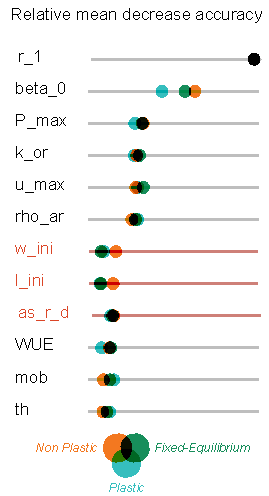
\includegraphics[width = \textwidth]{./2_PP/Figures/Calibration/importance.pdf}
\caption[Relative importance of main parameters for selection]{Relative importance of main parameters for selection under the three main allocation algorithms: (\textcolor{myOrange}{non plastic}, \textcolor{myGreen}{fixed-equilibrium} \& \textcolor{myBlue}{plastic}).}
\end{marginfigure}


%\begin{figure}[!h]
%   \begin{floatrow}
%\ffigbox{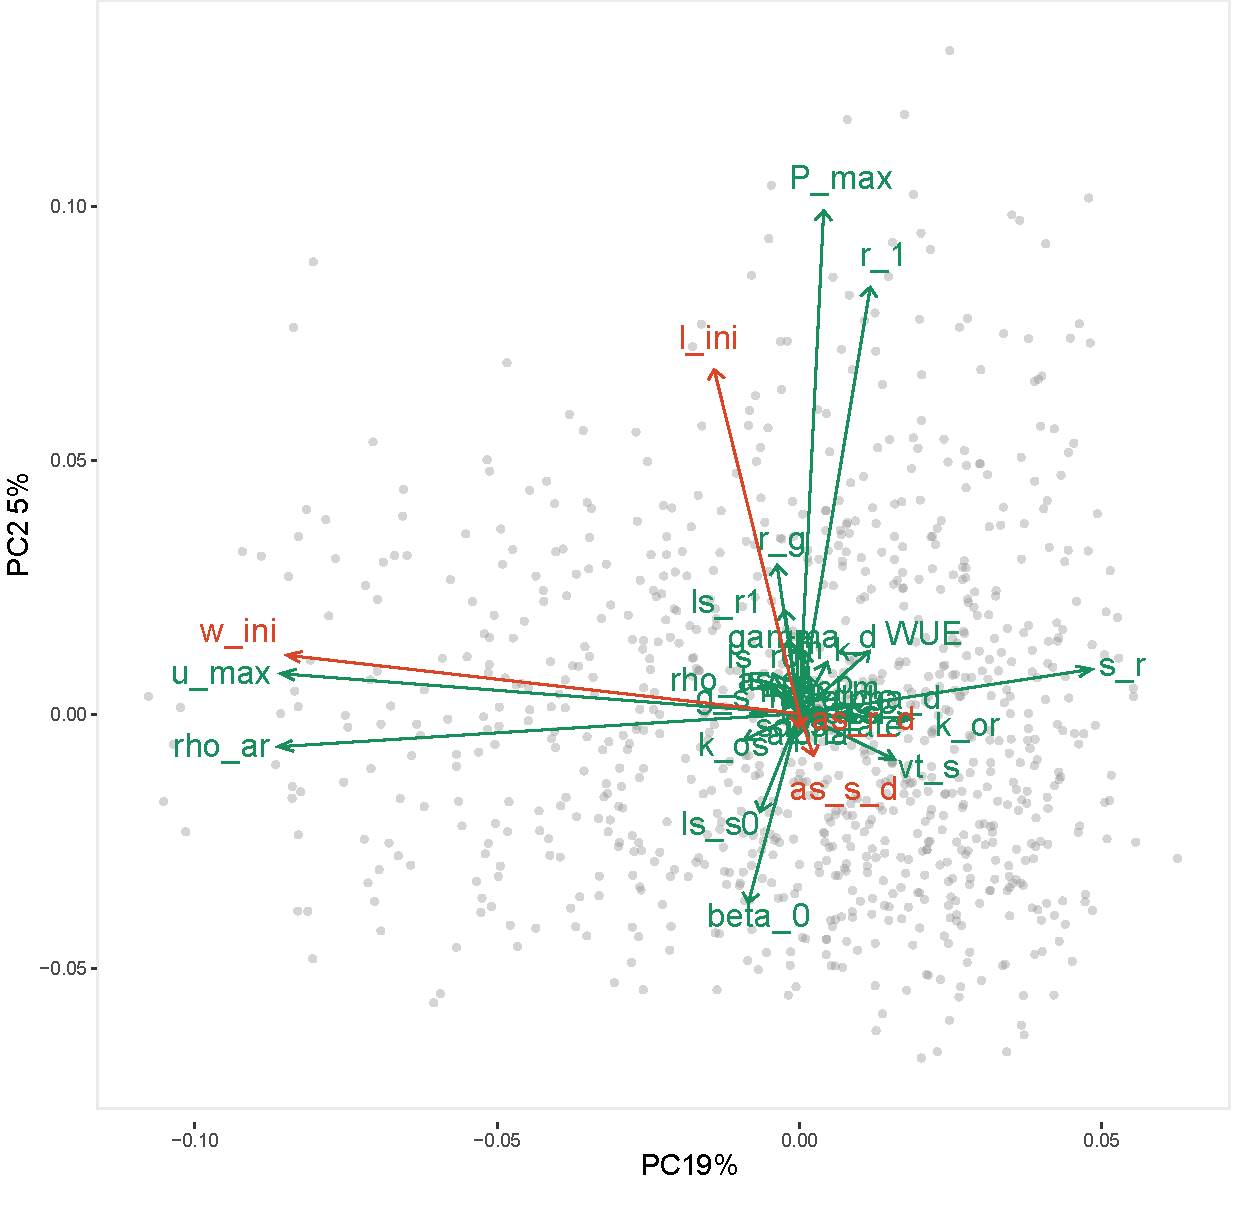
\includegraphics[width=\linewidth]{./2_PP/Figures/Calibration/PCA_none.pdf}}%
%\caption{First two axis of PCA of parameter sets selected in parameter filtering process. \textit{Non plastic}.}\label{fig:PCA_calibration}
%%       {\caption{second figure}\label{fig:example-2}}
%   \end{floatrow}
%\end{figure}
%\lipsum[3]

\begin{figure}%[tb]
    \classiccaptionstyle
\sidebysidecaption{0.60\textwidth}{0.3\textwidth}{%
    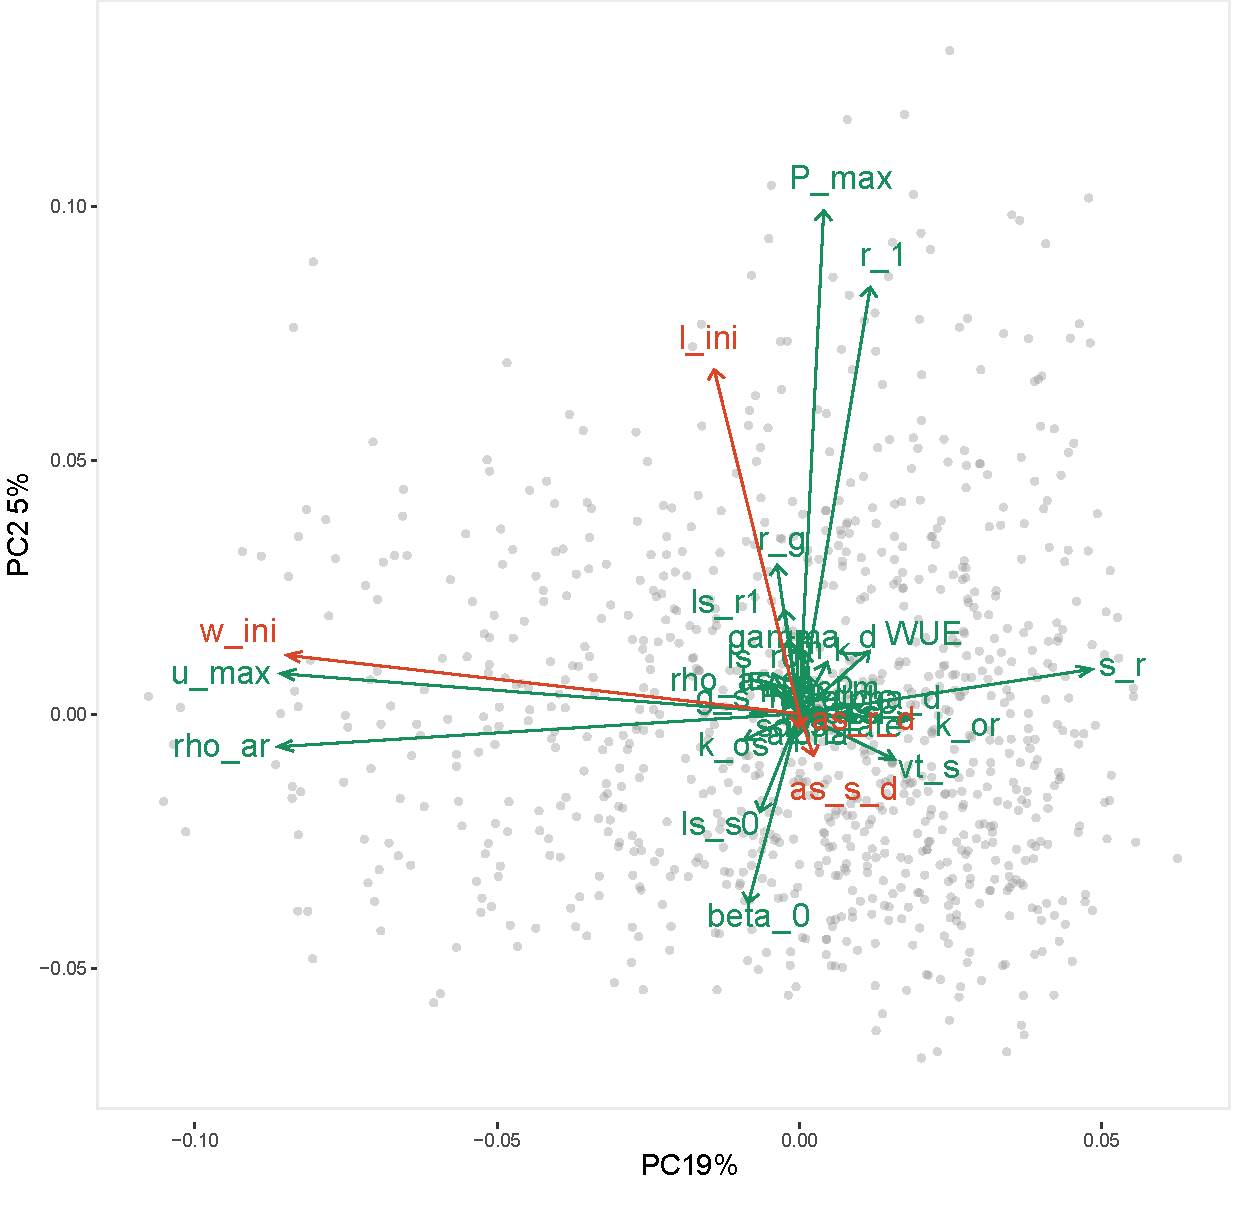
\includegraphics[width=1\linewidth]{./2_PP/Figures/Calibration/PCA_none.pdf}%
}{%
  \caption[PCA calibration]{Representation of the PCA of parameter sets selected in parameter filtering process on the first principal components. \textit{Non plastic}.}
  \label{fg:PCA_calibration}
  }
\end{figure}

The PCA performed for \textit{non plastic} algorithm only on parameter values reveals that important parameters are also the dominant variables that shapes the selected subspace. The two first axis explain only 14\% of variance. The first one is related to the root activity and efficiency (\texttt{u\_max}, \texttt{l\_ini}, \texttt{rho\_ar} and \texttt{s\_r}), the second is in line with global efficiency and resource availability.

The parameter filtering process is based on individual species, ... Species cannot be distinguished on these two main component space, neither on species specific parameters space (\texttt{l\_ini}, \texttt{w\_ini}, \texttt{w\_ini} \& \texttt{l\_ini}, \texttt{as\_s\_d}, \texttt{as\_r\_d}, \texttt{as\_r\_d} \& \texttt{as\_s\_d}) despite small variations in distribution shapes and ranges between species (data not shown).\\

\paragraph{Variable responses}
% Response of the two main vairables to main parameters.
For each algorithm the response of the two filtering variables (weight and RSR) are plotted against the most important variables in figures \ref{fig:sensitivity_BM} and \ref{ fig:sensitivity_BM}.

% Biomass
Total biomass is particularly sensitive to tissue respiration cost (\texttt{r\_1)}, but also maximum exchange rate parameters. There is a notable difference in growth maxima between the two conditions in favour of wet conditions, in line with observed data. This difference is observed for the three algorithm that differ mainly by the amplitude of the biomass ranges (need data).  Growth response curves are similar for all allocation algorithm. Growth is only weakly related to species specific parameters. Total biomass under \textit{Plastic-optimisation} algorithm seems to be more sensitive to variables influencing the exchange area per unit of biomass.

The species specific parameters \texttt{tau} controlling the balance between genetic and environmental control does not emerge as a influencing parameter at the global scale for any of the two flexible allocation rules.

\begin{figure}\label{fig:sensitivity_BM}
\includegraphics[width = \textwidth]{./2_PP/Figures/Calibration/par_effect_none_BM.pdf}
\caption{Main parameters effect on the total plant biomass. \textit{Non plastic}. One dot represents a parameter set. Not all parameter set are represented as the y axis is limited around the smooth function (loess). Coloured points represent selected parameter sets in the two treatments (\textcolor{myOrange}{dry} and \textcolor{myGreen}{wet}).}
\end{figure}

% RSR
Root:Shoot Ratio (or RMF in figure \ref{fig:sensitivity_RSR}) strongly responds to species specific parameters under \textit{non plastic} allocation because the memory parameters(\texttt{l\_ini} and \texttt{w\_ini}) are the means plants control their RSR. For other allocation rules, species specific parameters have little control over RSR. Surprisingly, the photosynthetic capacity has stronger influence on the ratio than the root maximum exchange rate.


\begin{figure}\label{fig:sensitivity_RSR}
\includegraphics[width = \textwidth]{./2_PP/Figures/Calibration/par_effect_none_RSR.pdf}
\caption{Main parameters effect on the total plant Root Mass Fraction (RMF). \textit{Non plastic}}
\end{figure}

% TAU

\paragraph{Root shoot ratio and plasticity}

Little to no difference in RSR is expected for \textit{non plastic} allocation rule since allocation promoted a fixed phenotype, but both \textit{fixed-equilibrium} and \textit{plastic-optimisation} allocation rules allow for changes in RSR. Nevertheless, no stable change in RSR is observed in any of the simulations. Fluctuations are present but consist in stable oscillations between two fixed values (see figure \ref{fig:comparison_RSR}), synchronized with water variations. These rapid adaptations of the relative proportion of roots denote a high flexibility of plant phenotypes in \model.


\begin{figure}\label{fig:comparison_RSR}
\includegraphics[width = \textwidth]{./2_PP/Figures/Calibration/RSR_full_sim_f-e.pdf}
\caption{Comparison of simulated values of RSR with real species RSR in two contrasting conditons. Because there is no plasticity or ontogeny, the simulated plant do not express any chagnes in RSR.\textit{Fixed-equilibrium}.}
\end{figure}

\subsection{Discussion}

\paragraph{Growth and strategy space}

The relative low selection rates for all allocation rules highlight the complexity of fitting such complex model to empirical data, despite the relative simplicity of the data. This difficulty seems to lie in two factors: the high number of parameters and the lack of stable changes in RSR. This last point is further discussed in the following paragraphs. Nevertheless, plant growth is reproduced in two contrasting conditions for multiple species, and while plastic algorithms have a greater potential for growth (more high growth rate), this is not systematic and the absence of clear pattern for the most influencing parameters, such as maximum exchange rates and respiration rates, indicates that such high growth depends on a combination of parameter values. I believe that the shape of gain and cost functions along the functional trade-off between active and structural tissues plays a determining role in the growth. A trade-off function with a wider viable range is more likely to be selected as more strategies would grow (therefore reducing the relative sensitivity to species-specific parameters). Considering the exponential shape of the turn-over function (one of the main cost with respiration), the width and height of the trade-off (or net gain function) is probably more strongly linked to the gain functions (exchange rates) and linear cost function (respiration), explaining little effect of parameters related to lifespan (already preselected otherwise). There is a strong dependency between viable strategies (and as a consequence functional potential diversity) and the main trade-off between resource acquisition and efficiency.

Filtering the parameter sets based on all species instead of individually would have been ideal to quantify this link and better calibrate the model. However, such approach would have required many more simulations, when the parameter filtering method was chosen for its low computational cost. Moreover, considering the number of species-specific parameters, fitting the strategy subspace (at least default active tissue allocation parameters, the memory of resources and stability) of 11 species to the data in combination with more than 20 models parameters is near impossible. Ones should have had first determined the relative positions of the species within the said strategy space before any global calibration routine. Nonetheless, species-specific parameters have an influence on model main variables. Memory parameter affected the RSR in the context of \textit{non plastic} allocation rule (see figures \ref{fig:comparison_RSR} and \ref{ fig:importance}, while the default proportion of active tissues in roots was an influencing parameter in all algorithms (figure \ref{fig:importance}, \texttt{as\_r\_d}). Therefore, they should be analyzed in further simulations within the same set of model parameters.

Change in modelling paradigm. The Bayesian paradigm where the information is contained in data and revealed by the structure of the model. Go for simulation experiment approaches where the model is used as a simulation tool and results as new data. The emerging patterns inform us on the impact of the modelled mechanisms (even if they do not totally match the data). Model as an understanding tool.\\


\textbf{Growth is reproduced, but only for one species, not full strategy space.}

\paragraph{The role of water}

If the parameter filtering step did not result in the selection of optimum values for all parameters, it provides information on the main mechanisms influence plant growth. 
Indeed, the relatively high importance of parameters related to water shows the importance of the resource on the model behaviour. Both water availability (water absorption limitation, exchange rate) and root mass and construction parameters are important to match the empirical data. Considering that the calibration relies on experiment data of drought events, it is no surprise that parameters related to water economy show strong influence on the selection rate and model behaviour. In the context where the model has been developed, water shortage is expected to an important factor in community dynamics. In this perspective, the ability of \model to reproduce the difference in productivity in both conditions, and the relative sensitivity to water related parameters is an advantage. The link between water resource, species strategy, plant performance and phenotypic plasticity is explored more in details in the following section.


%Differences between algorithms that make sense: more biomass, sensitive parameters are related to how plasticity work...

\textbf{Sensitivity of different variable to the parameters make sense and align with the two criterion of selection (that work with the independence of trade-off).}

\paragraph{More complex plasticity?}

As mentioned earlier in this discussion, the model is not able to produce any shift in RSR in different water treatment. It is not a surprise for \textit{non plastic} algorithm, but the filter was still applied on this criterion to allow the comparison with plastic algorithm and to be able to measure the improvement in selection rate. However, even plastic algorithms do not show strong enough response to water treatment in term of RSR. A strong and good (in the sense it would have matched the data) is larger in amplitude and more stable in time. Such processes generally amplify with time, \textit{i.e.} when the number of drought event increases, the response (allocation to roots) increases (relative to default phenotype). Unlike natural systems, plants in \model fluctuates between two "states", or phenotypes associates to the dry and wet conditions. The RSR post drought event is reached after the first week without water. This can be explained by two main mechanisms that are related but have contrasting implications. The quickness in response to the changing conditions is allowed by relatively high assimilation rate. If the net growth rate is controlled by the total weight condition during the filtering process, the assimilation rate is not and can be compensated with relatively high turn-over rate. Net growth rate being equal, species with higher assimilation rate will have higher phenotypic flexibility (higher fraction of biomass to invest in carbon pool of choice) than species with lower assimilation rate. This flexibility, similar to reallocation, allows changes in RSR, but not the accumulation of biomass in roots. Unfortunately, both the constant turn-over rate implemented in the model, and the selection toward "wide and high" gain functions limit control on this aspect.

Moreover, the fact that plants are more productive during periods where they may not want to invest in roots strengthen this effect. Indeed, a plant would drift to higher RSR if it was more productive when pursuing the high RSR phenotype than when pursuing the low RSR phenotype. This last point mentions the "will" of the plant, in the context of \model this target phenotype is encoded in the projection of external conditions. Because this projection is daily based by design, the accumulation of drought stress is not translated in the internal projection variables of the plant (like it can be with the accumulation of phyto-hormones \cite{need ref}). This limitation highlights a big difference between simulated plants in \model and natural plants. While solutions to overcome this problem can easily be imagined(see equation \ref{eq:projection_alt} in \ref{subsection:submodels}), they would require more parameters and introduce more complexity to the analysis. This model provides a first approach to phenotypic plasticity in grassland models and the formulation of the projection, key element of the phenotypic plasticity, is certainly a starting point for further development. Nevertheless, the differences in response to the parameters between the three allocation rules, despite shared plant functioning, demonstrate the importance of plasticity itself. And simplification of the processes should not be a reason to not explore its effects. The fact that the parameter \texttt{tau} has a relatively small impact on selection rates alos support the need to better understand all strategic axis before focusing on the effect of projection. While there are many ways of simulating the phenotypic plasticity, the parsimony is privileged. This simple representation is enough to understand the effects of active plastic allocation in association with the other strategic differences between species.


%Exchange area per biomass and sensitivity to exchange rates : trade-off are important and structuring.

%filtering on RSR to test if plasticity improved selection of parameters, = is an essential part of platn functioning.\\
\paragraph{Modelling paradigm}
Bayesian paradigm where the information is contained in data and revealed by the structure of the model. Go for simulation experiment approaches where the model is used as a simulation tool and results as new data. The emerging patterns inform us on the impact of the modelled mechanisms (even if they do not totally match the data). Model as an understanding tool.\\
%While many ways of simulating the phenotypic plasticity can be proposed, the parsimony is privileged and this representation is enough to understand the impact of related processes shared by any representation of phenotypic plasticity is the developed framework.

\textbf{Root shoot ratio changes were not captured by the model. The structure of the plasticity mechanisms does not work with the given watering cycle. Needs to add one parameter for reactivity.}



% ##################################################################################
\section{Individual level behaviour and properties}


Calibration and sensitivity analysis give information on the main processes of plant growth, but the general effects of the allocation rules on plant growth are not fully identified. In addition, because the parameter filtering processes was limited to individual plants, and the response of species specific parameters dependent on other parameters of the model, the effects of these species specific parameters should further be investigated. The objective of this part is to set better understanding on the role of \textemph{allocation rules} and species \textemph{memory} on plant development as basis for interpretation of plasticity effects in following chapters.

The challenge of the framework presented in paragraph \ref{subsection:memory} under \textit{plastic-optimisation} is to control the phenotype with the values of the memory. The risk of this approach is to have too tight estimation function of the fitness (or driving function) and to see the convergence of all species (with different memory values) toward the same phenotype (same allocation of active and structural tissues in roots and shoot). The extend to which different species memory lead to different phenotypes under full genetic control (non influence of external conditions) is explored through simulation experiment under \textit{plastic optimisation} allocation algorithm.

%Proof of concept
\subsection{Method}


%\paragraph{Strategy diversity filtering}
%To further reduce the number of parameter sets considered, we proceeded in an additional filtering step. Because the first filtering was conduced for only one strategy over the whole 4D strategy space (l\_ini,  w\_ini, as\_s\_d, as\_r\_d) it is necessary to verify that other strategies do not lead to potential Darwinian demon. This should be limited by the choice of priors, while at the same time promoted by the selection of parameters increasing growth to counter balance potential unfitted strategies\footnote{Better do that beforehand than after... But I guess it's too late now.}.

\paragraph{Allocation algorithms}
The effect of allocation rule on phenotypic development is investigated thanks to pot simulations (see Methods in \ref{section:calibration}) of 100 days in 3 watering treatment: 2mm, 8m and 16mm per day. To avoid drift in the phenotype due to allocation algorithm (see paragraph \ref{subsection:memory} on phenotypic determination), simulations where run a first time, then rerun with default specific traits matching traits at the end of the first simulation set. All four algorithms are simulated. To reduce the number of simulations 100 parameter sets are selected randomly within the accepted parameter sets for the \textit{non plastic algorithm}.

\paragraph{Memory \& phenotype}
Memory of external conditions plays a determining role in phenotypic development under \textit{plastic-optimisation} allocation rules. The effect of the memory alone (environmental cues ignored by setting \texttt{tau} to 1) on the default emerging phenotype is explored for diverse memories (9 values on the two axis from 0.1 to 1 later scaled to the maximum area exchange rates for model parameter set considered, or 81 values) for each accepted parameter set. The effect of the memory values on the final position of plants in the phenotypic space are visualised by fitting loess curves between memory values and individual trait values.

\subsection{Results}

\paragraph{Allocation rules}
think of a "showtime" visualisation that shows how growth and traits are impacted by allocation rules and \texttt{tau}.\\

Have the proportion of tissues changing over time\\

Show the respiration, assimilation and turn-over rates.\\ 

Isn't it possible to show these along memory or active/str ratio axis ?


\begin{figure}\label{fig:plastic_allocation_trajectory}
\includegraphics[width = \textwidth]{./2_PP/Figures/Individual/memory_effect.pdf}
\caption{Trajectories along time in the strategy space of 5 plants with different memories. After 10 days, all plants have converged toward the estimated optimum.}
\end{figure}

\paragraph{Memory and phenotype}

The kinetic of the phenotypic shift is first visualised for one parameter set on the two main phenotypic axis (proportion of active tissues in roots: PAR and proportion of active tissues in shoot: PAS). From the same starting point the five species show distinct rapid shift toward segregated subspace of the 2D strategy space. The equilibrium point is reached in approximately 10 days for all 5 species. Despite constant memory, variations are visible on both tissue allocation traits of roots and shoot. These variations lead to partial overlap but the five species are distinct on the 2D space.

The memory of resource availability is a strong enough driver to alter the default phenotype of a species. The effect of the two components of the memory (memory of water availability and memory of light availability) on the three main traits is explored through local regressions. The proportion of active tissues in roots increases to a plateau with increase in water availability memory (figure \ref{fig:w_ini_p_as_r}). This response pattern is consistent between all parameter sets, but the starting points and slopes may differ. The same pattern is observed between light availability memory and proportion of active tissues in roots (data not shown). The allocation convergence in the root is also influenced by the increase in light availability memory. An increase in the latter leads to a smooth increase in the former (see figure \ref{fig:l_ini_p_as_r}) with less drastic response than the water. This response is mirrored in shoot allocation response to increase in water availability memory (data not shown). Both organs react in symmetric ways to increases in resource availability. The RSR has a negative log response to water availability memory (positive in the case of light availability memory).

\begin{figure}\label{fig:w_ini_p_as_r}
\includegraphics[width = \textwidth]{./2_PP/Figures/Individual/w_ini_p_as_r.pdf}
\caption{Effect of memory of water availability on proportion of active tissues in roots. \textit{Plastic-optimisation}. Each line correspond to a local regression fitted for all memory combinations for a given parameter set. Water availability memory is given in percentage of maximum exchange rate, absolute values may change between parameter sets.}
\end{figure}


\begin{figure}\label{fig:l_ini_p_as_r}
\includegraphics[width = \textwidth]{./2_PP/Figures/Individual/l_ini_p_as_r.pdf}
\caption{Effect of memory of water availability on proportion of active tissues in shoot. \textit{Plastic-optimisation}. Each line correspond to a local regression fitted for all memory combinations for a given parameter set. Light availability memory is given in percentage of maximum exchange rate, absolute values may change between parameter sets.}
\end{figure}

The combine effect of the two axis of plant resource availability memory is observed by plotting the phenotypes (on the 2D space of active tissue allocation) of four contrasting memories for all parameter sets (figure \ref{fig:memory_n_phenotype}). There is clear clustering of the four memory profiles, with some overlaps due to the fact that multiple parameter sets are plotted at the same time. The memory of low availability (\textcolor{myRed}{$\bullet$}) has a much larger distribution area than others, suggesting the relative instability of this profile within the "estimated net gain landscape". Memory of low availability for both resource drives plant toward very conservative strategies (need some values here) than other strategy. High expected availability of at least one resource increases allocation to active tissues to both organs. This confirms the positive effect of complementary resource (light for roots and water for shoot) of active tissue allocation in organs (see figure \ref{fig:l_ini_p_as_r}). Because of this, there is no highly unbalance phenotypes with high contrast between organ specific allocation emerging from the \textit{plastic-optimisation} allocation in \model. There is general coordination, but the balance between resource availability memories still impacts the position on the 2D, illustrated by the absence of overlap between low light - high water  (\textcolor{myBlue}{$\bullet$}) and high light - low water (\textcolor{myYellow}{$\bullet$}) phenotypes. In case of high resource availability and coordination, high investment in active tissues for both organ is achieved(\textcolor{myGreen}{$\bullet$}) and high light - high water), but the range of values is similar than for unbalanced memories(\textcolor{myBlue}{$\bullet$}) and high light - low water (\textcolor{myYellow}{$\bullet$}).

\begin{figure}\label{fig:memory_n_phenotype}
\includegraphics[width = \textwidth]{./2_PP/Figures/Individual/par_v_2D_points.pdf}
\caption{Impact of species memory on final phenotype in case of fully plastic allocation. \textit{Plastic-optimisation}. Each point corresponds to a plant phenotype for a memory syndrome for a given parameter set. Colours denote the memory syndromes.

\textcolor{myRed}{$\bullet$ low light - low water}, 

\textcolor{myYellow}{$\bullet$ HIGH light - low water},

\textcolor{myBlue}{$\bullet$ low light - HIGH water},

\textcolor{myGreen}{$\bullet$ HIGH light - HIGH water}.}
\end{figure}



\subsection{Discussion}
\paragraph{Allocation rules}

rapid convergence.\\

Cost and gains\\

Diversity of phenotypes\\

Crossed and symmetric influence: the respective efficiencies cannot be analysed independently.\\



\textbf{Allocation rules are extremely important as they reduce the phenotypic space explore. Without even considering plasticity. Need a good understanding of the performance within the phneotypic landscape. Plus there is a need for alignment between starting phenotype and endpoint. Will also affect how plasticity is driven.}

\paragraph{Fast-slow strategies}

... nothing here yet, the idea was to show that the "strategy" of the species conduce to slow and fast archetypes. Should be able to show that with some memory simulations.\\

But not equal distribution along the axis probably.


\textbf{Allocation trade-off allow for strategies from the fast-slow spectrum to arise, independently for shoot and root, in coherent framework. Potential effect of other strategy axis can be analysed alongside this trade-off, even if they affect composite traits like SLA or SRL.}

\paragraph{Memory and phenotypes}

 The symmetry and the curves shapes suggest that resource related organ is more sensitive and that "apparent" increase in resource availability promote more exploitative strategy. - what mechanism ?\\
 
It seems that there is greater concentration around high values of active tissues. This is consequence of net gain curves. Is this verified in other allocation rules ? Or is this an artefact ?
 
The role of memory highlight the expected problem of matching default phenotype with memory: little ontogeny effect (due to high growth and turn-over rates) and problem with distance based plasticity cost (would require a moving cost, instead of fixed reference cost).

For each parameter set the alpha shape of the volume could be drawn to have an idea on how parameters impact potential functional diversity. But no time here to test that.


\textbf{Memory is a strong enough driver to control plant organ strategy. The effect of overall activity should be studied too and considered if memory is used to determine the default phenotype.)}

Role of allocation rule and changes in traits, traits affect strategy and performance, memory lead to different phenotype/strategies (based on gain function), there is coordination, effect of complementary resource. Need to better understand allocation rule and optimum strategy, and convergence and diversity. 

\textbf{I REALLY NEED TO EXTEND THE CONCLUSIONS AND GO BEYOND MY OWN WORK. REFER MORE TO OTHER PEOPLE WORK ! ! !}

% ##################################################################################
\chapter{Individual performance, plasticity and variable conditions}

The previous section highlighted the ability of the model to model growth, but also the importance of species specific parameters. While the plasticity mechanism did not replicate to a full extend (stable and higher amplitude) the phenotypic changes between the  different conditions), there were some changes both in traits, and in growth leading to a higher selection rate. Considering the importance of species specific parameters and their potential impact on growth, these differences between plastic and non plastic allocation rules should be investigated in an extended manner. The specific roles of strategy and memory on the multiple components of plant growth need to be disentangled to draw better hypotheses on the role of phenotypic plastic on plant performance and coexistence. The role of resource availability on these mechanisms also needs to be interrogated. The effect of plasticity on coexistence can also be approached with respect to relative performances and contraction of the strategy space.

This chapter tends to answer these questions with simulations of individual plants with diverse strategies and under multiple allocation rules. To simplify the approach and focus on the interaction between species strategies and allocation algorithm, the plasticity will be model as discrete mechanism (tau = 0 for all plastic allocation algorithms).

\section{Individual performance: between strategy, memory and plasticity}

This first subsection focuses on the link between the phenotype and the plant performance. The plasticity and allocation mechanisms can affect both the link between phenotype and performance and the distribution of the existing phenotypes.



\subsection{Method}

\paragraph{Parameter sets}
Because little differences are found between accepted parameter sets for the three main algorithms, parameter sets selected for the \textit{non plastic} algorithm are used for all algorithm. To reduce the number of simulations but have a measure of the genericity of the observed patterns, 20 parameter sets are selected among the accepted parameter sets for the \textit{non plastic} allocation algorithm. As mentioned in the previous section, the parameter sets have been selected for only one species-specific and therefore an additional step was used to filter out the parameter sets that could lead to high biomass values. For each parameter set, simulations of diverse phenotypes run for 100 days of 15 hours with favourable temperature conditions (20 \celsius) along resource availability gradient. The parameter sets are selected based on the maximum biomass of all simulated plants. One parameter set is randomly selected for each of the 20 brackets between 0 and 2 grams of total biomass.

\paragraph{Strategy space sampling}
To better understand what make a plant perform in the model, a multitude of phenotype needed to be tested. Tested phenotypes are distributed regularly along the three axis of the strategy space (proportion of active tissues in root, proportion of active tissues in shoot, proportion of roots) between extreme values (respectively (0.1, 0.99), (0.1, 0.99) and (0.1, 0.9)) for a total of 3375 combinations ($15^{3}$).  Because the RSR is defined by the memory, and in this set of simulation experiments the RSR is defined before, the species memory needs to be computed afterwards. There is an infinite number of couple of memory values that can match a given RSR. Also, the projection of conditions is sensitive to both memory and experienced conditions, therefore the choice of memory can affect the relative sensitivity of species to changes in external conditions and alter the model behaviour. Because the role of memory is not the focus here, and because there is much more focus on the role of the plasticity as a mechanism (as opposed as a strategy with various values of \texttt{tau}), the parameter \texttt{tau} is set to 0. This ensures that only the starting phenotype and the experienced conditions play a role in plant performance.

\paragraph{Simulation set-up}

For each phenotype a pot simulation is ran for 100 days of 15 hours under 4 millimetres rainfall and 120 Watt per square metres and per hour with the 4 main allocation algorithms (\textit{non plastic}, \textit{fixed-equilibrium}, \textit{fixed-optimisation} and \textit{plastic-optimisation}. Two resource levels are tested for each simulations. The low resource availability conditions correspond to a reduction by a factor 4 of resource influx, but the day length was conserved.

\paragraph{Projections}

To visualise the performance landscape (plant performance relative to biggest plant as function of its phenotype) the performance of best phenotypes are projected against the 3 plans that compose the phenotypic space. Such projections are preferred to 3D alternatives as they work better with static visualisation and when most of the space is occupied. Alternative axis are defined to facilitate the interpretation and description of the performance landscape. The organ strategy plane(PAR-PAS plane) can be transformed into strategy balance (difference between PAS and PAR) and "speed" (in sense of Reich \cite{reich_world-wide_2014})(mean allocation to active tissues).

\subsection{Results}

\paragraph{Performance landscape}
 On the tissue allocation plan (proportion of active tissues in leaves and roots), the best performing phenotypes present a bean shape. This shape suggest that relative importance of organ efficiency is lower than other criterion such as equilibrium and overall performance (see section \ref{chapter:modelling_PP} paragraph \ref{subsection:match} for the discussion on the components of plant performance). On this plane, the lowest values of plant biomass are characterised by low values of active tissue allocation. 
 
Phenotypes with high active tissue allocation values tend to have lower growth values than phenotypes with similar values for one of the organ and lower value for the other organ. 

Projection of the best phenotypes over the three planes also gives information on the importance of the ignored variable on each plane. The greater the discrimination of the subset of best strategies on a given plane, the lower the importance of the ignored plane. The projection on PAR-RMF and PAS-RMF planes discriminate better phenotypes relatively to PAR-PAS plane, therefore the RMF is a more important variable than allocation to active tissues in organs.

If equilibrium is a driving mechanisms in plant performance, for any given strategy (PAR-PAS plan projection) the best phenotypes has a RMF values that guarantee the functional equilibrium. However, for each strategy there is a notable difference between the RMF of best phenotypes  and the RMF of phenotypes the closest to the equilibrium. This disparity is positively related to the strategy balance: best phenotypes with higher active allocation in shoot than root have lower allocation to roots than required for functional equilibrium. 

Higher resource: contraction of the landscape, toward faster species. Moving optimum and moving gravity center. Transition to optimum shifting and difference between allocation rules.

\paragraph{Optimum shifting}

Shift due to plasticity (toward higher RSR) -> timing only ?
+ shift (not fully significant in high resource availability) toward more exploit shoot and less exploit root. What does that mean ? higher tissue efficiency authorized by less limiting water ?

Where is the optimum ?  what makes an optimum ? Why is it important ? -> beter understand how plasticity works and can improve plant performance.

What are the sensitive dimensions ? and why ? 

then moving optimum and why ?

Moving optimum 2D: why ?

What is the plastic-optimisation doing ? Wrong phenotype ? Wrong projection ? Wrong strategy or wrong RMF ? 


\begin{figure}\label{fig:w_ini_p_as_r}
\includegraphics[width = \textwidth]{./2_PP/Figures/Landscape/plot_BM_allocation.pdf}
\caption{Effect of plasticity and resource availability on average biomass of living species.}
\end{figure}

Biomass is relative to best performing non plastic plant (to remove the general parameter set effect on growth) and compare (within each condition) the effect of allocation algorithm. Plasticity lead to an increase of average relative biomass, especially full plasticity. However, few values above 1, in fixed conditions there is real additional value of plasticity compare to fixed allocation.\\

\paragraph{Phenotypic convergence}

Shifts in optimum, is it because plasticity provide more efficient functioning supporting more exploitative strategies, or side result from convergence that do not contain the previous optimum ?

Convergence, relative species diversity and functional diversity.




\subsection{Discussion}

\paragraph{Components of performance}

To understand how plasticity can play a role, it is important to understand what make a phenotype a good phenotype. In an other way it is important to understand what cost do a plant for being wrong.

\textemph{equilibrium}, overall \textemph{speed} and overall \textemph{efficiency}.

Better too fast than not fast enough.

Explain the memory stuff in previous section: low-low compared to low-high, the second one lead to overall higher productivity (lack of one resource compensated by higher allocation to the related organ) that can support more active tissues. 


\paragraph{Convergence to subspace}

Phenotypic plasticity is often perceived with a species-centric perspective, that is to say, that plasticity is seen as variations in the species mean phenotype. However, in the context of community ecology, it is also interesting to try to see how it not only affect individual species but shape the community distribution in the strategy space. Plasticity relies on changes of default phenotypes toward "better" strategies in the context of the given conditions, therefore it implies that if it exists an optimum subspace (one strategy or an ensemble of strategies) species will converge toward this subspace, distorting the functional space. Environmental variations and plant interactions aside, in a constant environment the \textemph{performance landscape} is fixed. As a consequence the plasticity benefits to the plant in a static manner, that is to say, it is only a tool to reach a better phenotype where the plant stays in if conditions do not change. This can be related to spatial heterogeneity that would lead individuals from the same species to adopt different phenotype to acclimate to the particular conditions of their spatial situation. It is opposed to the perception of a more dynamic phenotypic plasticity as a tool for a given individual to cope with temporal variations in environmental conditions. These two aspects are further discussed in the following section, while the effects of the contraction of the phenotypic space are discussed now.

As explained before, plasticity can be seen at the scale of the species assembly \sidenote{here I draw a distinction between species assembly that refers to all present species, and community that refers to the interacting individuals of the present species. However, some interpretations can be translated to communities.} as a contraction of the phenotypic space of the species assembly. This contraction has two main effects: the reduction of potential functional diversity and a reduction of growth rate differences. There is here an emerging trade-off between the species diversity, supported by lower fitness differences, and functional diversity, reduced by the contraction of the phenotypic space. However, if the plasticity reduces greatly the potential functional diversity (volume of the whole phenotypic space without considering filtering based on relative fitness), the realised diversity (expressed as the functional diversity of the species within the 90\%-100\% maximum biomass range) is much less impacted because a large part of the phenotypic space (explaining the large potential functional diversity) has low growth rate in the given conditions. Nevertheless, the reduction of the diversity of expressed phenotypes is greater than it could ideally be. Indeed, in this scenario of "extreme" plasticity ($\tau = 0$) the convergence is important on plastic dimensions where it is not needed to have a significant increase in fitness (see conceptual figure \ref{fig:convergence}). Lower convergence on plastic dimension should lead to less compact phenotypic subspace while keeping relative fitness evenness. In the case of \textit{fixed-equilibrium} and \textit{fixed-optimisation} plasticity mechanisms, this effect is reduced by the sensitivity of the growth rate to the unique plastic dimension (see figure \ref{fig:plane_projections}). ... About \textit{plastic-optimisation} convergence...

Cost and distance, sensitivity to environmental cues as solutions to this problem. 

Because of high convergence of \textit{plastic-optimisation}, no improvment of maximum biomass, but the \textit{fixed} alternative thanks to convergence limited to one phenotypic dimension (RMF) higher biomass: either higher resolution, or improvement due to \textemph{dynamic plasticity}. The role of dynamic plasticity benefit is explore in temporal variation simulations in the following section.

\textemph{Convergence}

Somehow I need to talk about the cost of being wrong. Can be observe in the delta heatmap on delta strat and delta w-ini: in this case there is less impact of being wrong of memory if you're good with strategy, because your not in different conditions...\\

Potential effect on diversity: lower functional diversity, increase evenness. Leave highest fitness spot free. Why ? environmental cues or gain function ? Delta between projections ? \\

Anyway, being good is stable conditions may useless if cannot survive or keep gain in other conditions. >> look along gradient if best species keep their rank.\\

\paragraph{Wrong proxy?}

What happen to plastic plants ? Wrong phenotype ? Wrong \textemph{projection} ? Wrong strategy or wrong RMF ? 

\paragraph{Nuances around plasticity}
This analysis was conduced with drastic parameters of plasticity with plastic plants relying only on their perception of external conditions to develop their phenotype. The different results ... different directions and impact on potential diversity.\\
The contrasting responses of the different algorithms highlight the importance of the allocation mechanism. However, the unique framework implemented in \model creates a variety of nuanced responses that are not all explored here. But, the continuous gradient of strategy between species relying on species memory only and species following their perception of external condition should be kept in mind during the interpretation of these results and following.

\paragraph{Resource availability}

results from this part\\
As expected the resource availability and the resource balance are key components of the plant growth, to which the plant phenotype needs to match. Aside from the increase in biomass, an increase in "speed" of optimum phenotypes can result from higher resource availability. This observation is in agreement with empirical data that demonstrate higher SLA and faster physiology in favourable conditions. This aspect was less obvious in the response of species under \textit{plastic-optimisation} allocation that shifted more in term of balance and RMF. This may be due to a change in the relative balance between both resources as their availability (from the plant perspective) are linked to the global resource levels by non linear relationships.

The fact that plastic plants (for \textit{fixed} allocation algorithms) show shifts of optimum strategies toward more exploitative phenotypes, in addition to the \textit{non plastic} optimum shifts, in conditions of higher productivity demonstrate the importance of these strategies for plant growth. However, the extend of this effect of conditions on optimum phenotype is succeptible to vary along a gradient. Indeed, because of the non linearity of relationships between resource levels and exchanges rates, and between exchange rates and growth rates, the link between the optimum phenotype and a resource gradient is likely to be non linear itself. In addition, phenotypic plasticity might also change the sensitivity of the phenotype to the resource level.

Why we need to go for a gradient.

\paragraph{Greater level discussion}
? about what ? Community dynamics ? pp impact of these dynamics ? coexistence of species


\textbf{Subsection conclusion: bla bla bla}


% ##################################################################################
\section{Plasticity and variability of conditions}
Question I try to answer: (use of schematics ?)
The heterogeneity of conditions is an essential mechanism for plant coexistence. Plasticity is likely to alter the effect of this heterogeneity on plant interactions and relative performance. The impact of plasticity on this relationship between spatial and temporal \textemph{heterogeneity} of resources (here limited to water) and strategy dominance is explored with the model \model.

\subsection{Method}

Because little coordination, and importance of below-ground resource acquisition (in the results, and in the context) and computational cost - only root strategies.

\paragraph{Simulation set-up}
For each of the 20 selected parameter sets, growth of 400 plants (20 PAR values between 0.25 and 0.95, and 20 memory values between 0.1 and 1) is simulated for 100 days in square pots of 12 centimetres deep and 90 centimetres wide (to avoid quick self-competition) in a temperature of 20 degrees celsius during the day of 15 hours, and 10 degrees during the night. Irradiance is set to the high values of 122 Watt per hour and per square metre. 

\paragraph{Spatial heterogeneity}
Spatial heterogeneity of water level is mimicked by a gradient of water influx. The growth of all 400 species described above are simulated for \textit{non plastic} and \textit{fixed-equilibrium} algorithm independently in separated simulations where the water influx is regularly sampled between 0.05 and 7 mm per day (20 values).

\paragraph{Temporal heterogeneity}
Similar set-up is used for temporal heterogeneity simulations. Because the range of water influx used in the previosus simulation is too wide, a lower value is chosen as the mean water influx. This value of 1.3mm per day corresponds to a point around which there is vairations in the optimum strategies for most parameter sets. It is also relatively close to average rainfalls in the Alps during summer. 

\subsection{Results}

\paragraph{Optimum strategy}

\paragraph{Survival}

\paragraph{Diversity}


\subsection{Discussion}

\paragraph{Improvement in variable conditions}

\textbf{Phenotypic plasticity }

\paragraph{Heterogeneity of response}

Kichenin (different response to gradient) Doesn't work in this framework: Not so sure about that: depending on your initial memory plants show directional changes toward one phenotype. Yeah, but they should have converged for other conditions too... So, it doesn't work. Might be explained by:
\begin{itemize}
\item different conditions: because heterogeneity and habitat selection, or changes in competition hierarchy;
\item different ways to tackle changes on one dimensions;
\item different weights between mechanisms impacting composite traits, because of the different traits.
\end{itemize}


\paragraph{Plasticity as a strategy}
One of the argument to say this is new, however not really explored, neither with plasticity cost perspectives (a bit with plasticity limits) or with tau. However, used extreme cases: give better understanding and necessary before finer analysis. Still, there are hypothesis on the effect on diversity and the role in phenotypic stability (attention: isn't it just because the formulation of projection is wrong that we can make these conclusions ?).



\paragraph{Extended interpretations}
What about the continuous $\tau$ gradient ?\\
What about interactions and cycles ?



\textbf{The phenotypic plasticity implemented in \model improve the relative performance of multiple strategies by concentrating the plant toward a subspace of higher performance for most of plants. Convergence to a smaller subspace can be assimilated to reduction in phenotypic diversity, but it reduce performance heterogeneity and should favour local plant diversity. .. a few words on dynamics... Meta-community diversity is however reduces by the reduction of potential axis for niche differentiation. Plasticity costs and limits should play major role in the balance between these mechanisms. Community level simulations are needed to further understand the cumulative role of competition, spatial and temporal variability and plasticity costs on phenotypic plasticity influence on plant community dynamics.}

%\section{From individual response to community dynamics}

% Use these notes to extend the discussion and add some outlooks
%
%\section{Niche response}
%
%
%Obj1: understand how resource use mechanisms and allocation algorithms shape the environmental potential niche in the context of the model.\\
%H1: strategy and memory affect niche in two ways if we suppose they are independent: shape and position. Strategy mostly affect shape (width and height) while memory (and so root:shoot ratio) affect mostly position.\\
%H1': there is strong link between strategy and memory in the case of optimisation allocation that increase niche height and might reduce its width.\\
%Obj2: understand the role of plasticity on the niche and if the effect in the same for all strategies/memories.\\
%H2: the plasticity increase niche width but not height (as phenotype is optimum at the center of the niche where memory match the resource availability).
%
%Stability and efficiency trade-off. Niche heigh and width and relationship with the strategy. How does plasticity affect that ? Does it increase the height and widen niches ? What does that mean for coexistence ?\\
%Hopefully higher niche would go with unstable niche.
%%
%%\section{Transitivity and competition}
%%1 vs 1 interactions\\
%%Is the resource competition transitive ? How does niche widening impact that, does plasticty change competition interaction. Is it related to the trait distance ? (don't think so)

%
%\chapter{The effect of phenotypic plasticity on plant community dynamics}
%Hypothesis on the cumulative effect on niche and interactions.
%
%\section{Individual resistance and resilience against drought events}
%Amplitude and length of the event :\\
%- severity effect reduced by lower tau ?\\
%- resistance versus resilience: H0: conservative strategy have higher resistance, H1 : low tau allows for re-equilibrium and increase resistance (low amplitude and long length. H2: high tau allow to avoid dead-end situation during short severe drought (high resilience)
%\section{Community response to drought event}
%coexistence effect vs resistance/resilience effect\\
%uniform vs heterogenous (plasticity wise) community response
%H1: 
%

\begin{fullwidth}
This second result chapter examines the effects of the phenotypic plasticity at the scale of the community. Another parameter filtering processes is performed and described in the first section of this chapter. The second part focuses on the effects of the plasticity on the main properties of the community. The impact of the plasticity on species diversity is particularly investigated. This chapter gives a glimpse of the potential of the model to answer various questions around the role of intraspecific variations on diverse community properties.
\end{fullwidth}

\chapter{Community level simulations: non plastic community}


\section{Parameter filtering}
\subsection{Method}

%\paragraph{Field data}
%Field data has been collected between years 201 .. and 201 by Claire Deleglise and al. (). Not used here.

\paragraph{Weather data}
Weather data for the time period between 1959 and 2014 has be computed by the MeteoFrance model SAFRAN by Verfaille Déborah using GPS coordinates, slope, azimuth and horizon computed from a digital elevation model. These parameters were also used by the model CROCUS to compute the snow accumulation and the snow melting. These high frequency data (resolution under 1h) have been averaged on a daily time-step and used to compute input variables for \model. The snow in particular defines the length of the growing season starting with the first snow melt of the year and finishing the day of the first snow fall during the autumn or winter.

Historical data is available between 1958 and 2014. The simulated years above 2014 are randomly sampled form the existing dataset between 1995 and 2014.

The six sites have been chosen to test the consistency of the parameters, and open the door to the exploration of the effect of the climatic variable. This last aspect is not developed in this manuscript.

\paragraph{Parameter filtering}
A community level parameter filtering is conduced for a new table of parameter sets. These parameter sets are all the from accepted parameters with 50 randomly sampled non accepted parameter sets, joined with a LHS random sampling for five community level parameters: seed germination density, drought mortality, ageing mortality, plasticity cost for environmental sensing and plasticity cost for trait changes (see chapter \ref{chapter:model-description} for details).

\paragraph{Simulations}
The simulations run over 300 hundreds years for 6 sites with similar soil depth, but contrasted climate, on squares of 2,500 square centimetres, under \textit{non plastic} allocation algorithm. After a stabilising phase of 50 years, the simulation is stopped and the parameter set rejected if no individual persist and the seedbank is empty. The seedrain is composed of seeds contained in the seedbank and seeds from the metacommunity. The total of seeds is defined by the seed germination density and the area simulated. The seeds from the simulated community represent up to 80 \% of the seedrain, less if the seed production is limiting. 400 species compose the meta-community with traits randomly sample from distributions estimated from the accepted parameter sets at the individual scale. This method can be discussed, but because only one species is evaluated for each parameter set at the individual level no parameter set specific distribution could be used and a shared distribution was preferred. This method still allows to avoid traits values that make no sense in any of the parameter set and reduces, even marginally, the number of potential non-viable species.



\subsection{Results}


\paragraph{Parameter filtering}

Among the  tested parameter sets, only 77 were selected after the parameter filtering process. 

Because too few parameter sets are selected with contrasted parameter values, no sensitivity analysis could be conduced to determined the key parameters of the model. For the same reason, the parameter effects are not detailed.

\paragraph{General behaviour}

While the main properties of the simulated communities are explored in the following subsection, the general community growth can be observed for these simulations. The individual profiles show a relatively high variability within the season, that is coupled with high inter-site and/or inter-seasonal variability for any given parameter set.
Despite variable growing-season starting dates, and some variability within parameter sets, the smoothed-profile show a consistent behaviour. This pattern is characterised by two distinct growth periods: (1) the initial growth  corresponding to the use of the stored resources, then followed by the growth promoted by the favourable conditions of the spring and early summer, and (2) another growth period at the end of the summer/autumn, following the growth reduction of the mid-summer. Two peaks can be observed during the first phase, but the first one is only noticeable for a few conditions where the season started early.  

\begin{figure}%[tb]
%    \classiccaptionstyle
%\sidebysidecaption{0.5\textwidth}{0.4\textwidth}{%
    \includegraphics[width=1\linewidth]{./2_PP/Figures/Comm/biomass_season_non_plastic2.png}%
%}{%
  \caption[Total biomass profile during the season]{Total biomass over time during the season. The small lines illustrate the individual seasons profiles (n = 20) for different sites (n=6) and parameter sets (colour). The growth profile of the different parameter sets are estimated with GAM models. The marks at the bottom indicate the beginning and the end of the seasons. \textit{Non plastic}.}
  \label{fg:species_per_plant}
%  }
\end{figure}

\subsection{Discussion}

\paragraph{Parameter filtering}

The parameter filtering process deployed here is sufiscient to select viable parameter sets allowing stable simulations. Ones could develop extended calibration plans to stabilise the behaviour of the model and ensure more realistic output. However, such approaches are mostly interesting when the model is it to infer information about specific, well described systems, instead of qualifying the general effect of freshly modelled mechanisms. The non reduction of the analysis of the model to one parameter set also increase the confidence in the observed pattern, and the conviction that they emerge from its structure rather than specific parameter interactions. Moreover, ambitious calibration procedure should rather be reserved to mature models, from which the general responses are well described and understood.

\paragraph{Driven by the weather}

The biomass profiles of the simulated communities show both consistency in the growth pattern, and high daily variability. The variability observed highlights the great the sensitivity to the weather variables. This sensitivity certainly favours positive effects of the phenotypic plasticity, if the changes in phenotype are responsive enough and do not suffer from a lag.

The consistent growth patter with two distinct growth period correspond to field observations where plants are generally divided between early flowering, matching the first biomass peak, and late flowering corresponding to an autumn growth and reproduction. This coherent behaviour, driven by the climate gives confidence in the integration of the climatic variables as drivers of the community. Further work could be done to confirm the respective role of the temperature and precipitation, but this work focuses on the effect of phenotypic plasticity and both the relative sensitivity to the daily variations in the conditions and the importance of the climatic variables as driving forces supposes that the plasticity has the potential to affect the mountain communities.
% sensitivity to the weather
% general climate driven response.

\textbf{The parameter filtering at the community scale ensure stability of the simulations at the community level. It also gives confidence in the global behaviour of the model, and in the driving role of the climatic variables.}
%\section{Non plastic communities}
%Trade-off, diversity, stability ...
%
%
%\paragraph{Ecological trade-off ?}
%Is there a selection of some parameters ? Are there ecological trade-off (resource use strategy and reproduction) emerging from the model ?

\chapter{Plasticity: impact on species fitness and diversity}

After a rudimentary parameter filtering, guaranteeing the stability of the communities, the effect of the plastic allocation algorithms can be investigated as the community level. As for the for the previous section, the focus is given to the main properties of the community: the diversity, the productivity and the identity. 
%
%Plasticity in integrated framework and full community simulations. Plasticity mechanisms, but also plasticity as a strategy (look at the cost and tau). 
%
%Effects on productivity and coexistence. Difference in the correlation ?
%
%Effect of tau on persistence.

\section{Plasticity and diversity}


\subsection{Method}

\paragraph{Simulations}
To test the effect of plasticity on coexistence and community dynamics, runs from the parameter filtering are used as starting points to limit the simulation time of the stabilisation phase. For each parameter set tested, 6 different sites were tested during the calibration phases, 77 parameter sets were accepted and a sample of 18 were tested, resulting in 108 communities. Each of those is the starting point of three parallel runs that differ only by the allocation algorithm used: \textit{non plastic}, \textit{fixed-equilibrium} and \textit{plastic-optimisation}. The \textit{fixed-equilibrium} is favoured to \textit{fixed-optimisation} algorithm because previous part of the document focused on this algorithm and because it is simpler to analyse. The \textit{plastic-optimisation} algorithm is still simulated, despite the relatively poor performance results observed in constant conditions and the high convergence, because the introduction of plasticity cost, continuous species specific plasticity ($0 < \tau < 1$), and temporal and spatial heterogeneity should mitigate the negative sides of this allocation mechanism and give information of processes at stake.

The plasticity costs (maintenance: related to the value of $\tau$, and displacement: relative to changes in phenotypes) defined in the parameter sets are applied to all algorithms. In the \textit{non plastic} simulations, this results in an artificial additional cost to all species, especially those with a low value for $\tau$, but with no potential gain from plasticity as the allocation is non plastic. This choice was made to ensure that the differences between the simulations are the results of the allocation algorithm only, and not a cumulative effect of the algorithm and the plasticity costs that could not be disentangled. This artificial cost can be seen as an artificial abiotic filtering process. Because 400 species are present in the meta-community, enough species with high values of tau should be able to invade the habitats, limiting behaviour emerging from low sampling.


%\paragraph{Statistical tests}

%The differences of effects between the different types of plasticity on the variables of interest are computed unpaired Wilcoxon tests assuming an independence of the the different data points. This assumption of statistical independence is justified by the normalisation for each parameter set of the variables relative to the mean of the \textit{non plastic} group. This normalisation allows to compare the simulations between the parameters sets. The interactions and other level (site, and autocorrelations) are discussed later in this section.

\paragraph{Normalisation}
To allow comparison between the datasets, the variables are normalised over the mean value of the variable under \textit{non plastic} allocation. So the \textit{non plastic} algorithm is the reference, but the variability caused by sites and seasons is still visible.

The normalisation $Vn_{a, p, t, s}$ of the variable $V$ for the allocation algorithm $a$, the parameter set $p$, the time $t$ and the site $s$ is given by the following formula:

\begin{align}
Vn_{a, p, t, s} &= \frac{V_{a, p, t, s}}{ \bar{V} }\\
\bar{V} &= \frac{\sum_{a == \text{\textit{non plastic}}}{} Vn_{p, t, s} }{n}
\end{align}

where $n$ is the number of observations for the \textit{non plastic} algorithm.

\paragraph{Species \& trait values}

For practical reasons the entire composition during the season are not store during the simulation process. The trait values are estimated \textit{a posteriori} from the reproduction pool composed of living individuals and seed produced. The species default values are use to compute the community weighted mean of traits with the living biomass or the cumulative seed biomass. Therefore, even if under \textit{plastic-optimisation} allocation the plants can change their trait values, these changes are not measured.

\paragraph{Diversity measures}

The diversity indexes are computed from the reproduction pool (defined above). The alpha diversity is simple expressed as the mean number of species per site and per year. The beta diversity is defined as the total number of species divided by the alpha diversity minus one. 

The abundance ranking is computed from the reproduction output, under the hypothesis that the reproductive output is proportional to the realised abundance and constitute a good proxy for the fitness.

\subsection{Results}

%Need to run the simulations. Script is almost ready, parameters are filtered from previous step.
%
%\paragraph{General behaviour} ?
%gradient along climatic gradient ? did I save the climate ? Nope, can't really say anything about it.

\paragraph{Effect on coexistence}

The level of coexistence is evaluated by the number of distinct species that manage to maintain at least one individual or produce at least one seed at the end of the season. This criterion allows to ignore the potential non stable diversity introduced by the meta-community invasion (sampling of species in the meta-community pool) and to consider species that can be filtered out due to seed mortality. The number of species increases in almost all simulated years and sites for both plastic allocation algorithms, with a median of 1.5 times the number of species in \textit{non plastic} simulations (see figure \ref{fig:species_richness}). This factor can go up to 6 for \textit{fixed-equilibrium} and 9 for \textit{plastic optimisation}.


\begin{marginfigure}\label{fig:species_richness}
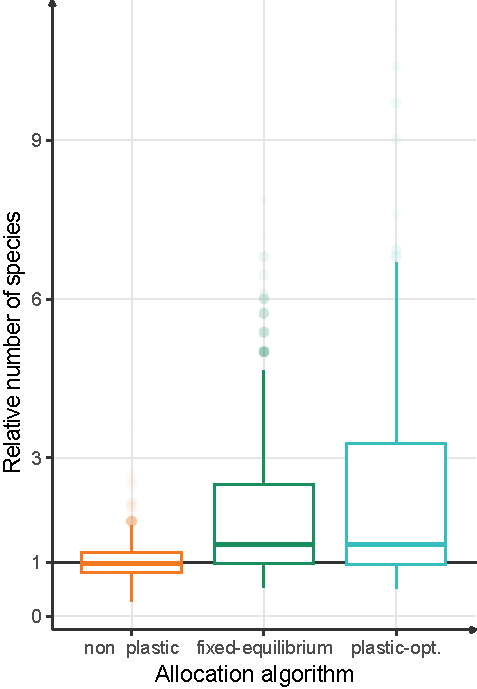
\includegraphics[]{./2_PP/Figures/Comm/comm_n_sp_differences.pdf}
\caption[Relative species richness in plasticity treatments]{Relative species richness in the three plasticity treatment. To negate the variability due to the parameter sets, the realised number of species is divided by the median number of species in \textit{non plastic} treatment for each parameter set. The variability is due to random invasion and climatic variability (inter-sites and inter-seasons).}
\end{marginfigure}

The effect of plasticity on coexistence is driven by the benefits of plasticity at the individual scale. These benefits are mitigated by the cost of plasticity, particularly the maintenance cost that affect all species relatively to their potential plasticity (proportional to $ 1- \tau$).

%Plasticity is responsible for high portion of variability, but also parameters: plasticity cost parameters:


Low values of plasticity maintenance cost (see figure \ref{fig:pl_cost}) show higher diversity for both plastic allocation algorithms. This trend is consistent across sites despites some inter-annual variability in the diversity. The effect is a bit less stronger for \textit{fixed-equilibrium} than for \textit{plastic-optimisation} (as already observed in figure \ref{fig:species_richness}). It is also important to notice that the cost of the plasticity has no negative impact on the coexistence levels for \textit{non plastic} simulations.

\begin{figure}%[tb]
%    \classiccaptionstyle
%\sidebysidecaption{0.60\textwidth}{0.3\textwidth}{%
    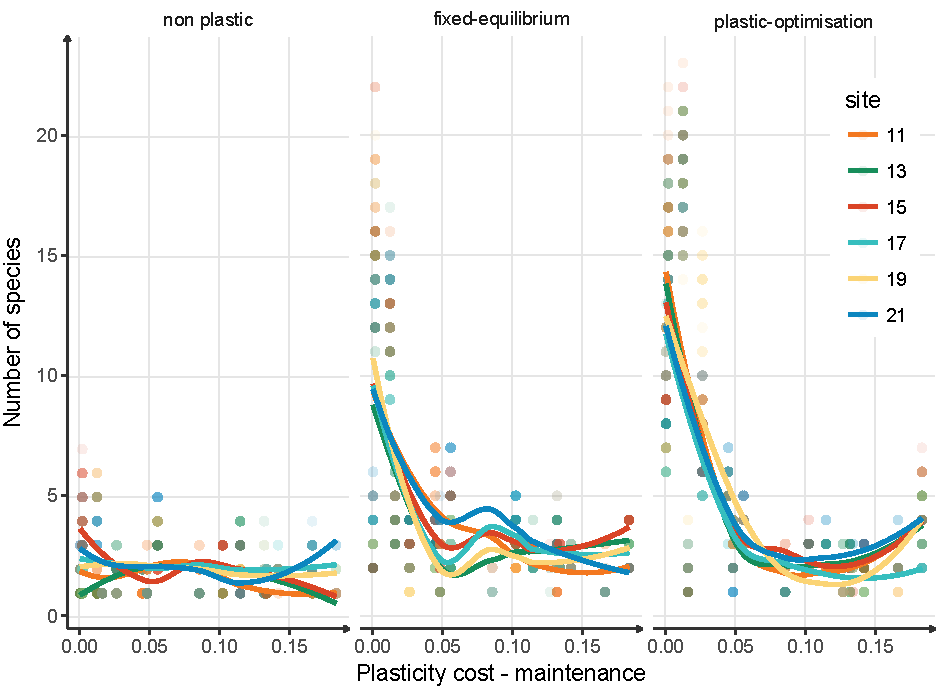
\includegraphics[width=1\linewidth]{./2_PP/Figures/Comm/comm_n_sp_pc_m_edit.pdf}%
%}{%
  \caption[Maintenance plasticity cost effect on species richness]{Effect of the cost of plasticity-maintenance on the absolute number of species in the three plasticity treatments. Individual season values (points) and site-specific trends (gam smoothing line) are represented. }
  \label{fig:pl_cost}
%  }
\end{figure}

%Consistent trends between sites. Inter-season variability (why didn't I save the weather?). Not super clean. Similar (but lower start) for plastic distance diversity. Can be because of interactions %or because non variable enough.

%Why higher diversity: it is not because of higher density (number of individual per m2).
%But changes in filtering: more species

The mechanisms through which the phenotypic plasticity impacts species richness are multiple (refer to the figure \ref{fig:plasticity-effect} in chapter \ref{part:literature}). However it is hard to disentangle them all.

The density can be affected by the phenotypic plasticity leading to higher species diversity\cite{lepik_high_2005}, leading to the sampling of more numerous species. The density, estimated by the number of individual after the reproduction phase (persisting individuals and produced seeds), is consistently higher in \textit{plastic} simulations (data not shown, but see figure \ref{fig:species_per_plant}). But the difference is relatively low (around 3\% higher than the \textit{non plastic} median density) and an order of magnitude lower than inter-annual and inter-site variations that can go up to 40\% difference relative to the median density (for any given parameter set).


%\begin{figure}\label{fig:tiller_density}
%    \classiccaptionstyle
%\sidebysidecaption{0.3\textwidth}{0.6\textwidth}{%
%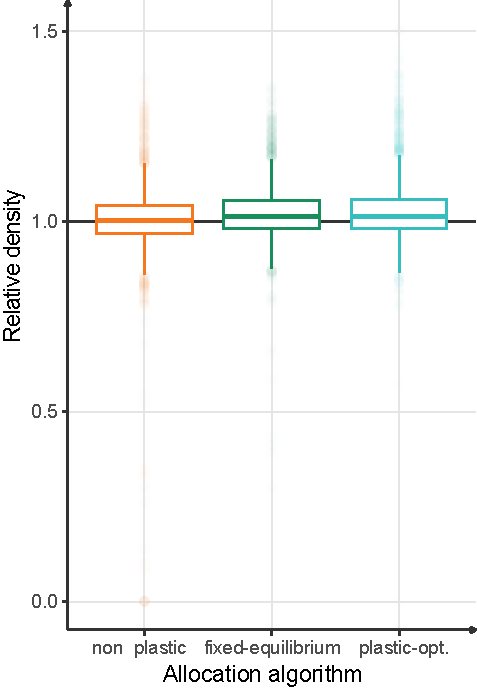
\includegraphics[]{./2_PP/Figures/Comm/comm_n_indiv_differences.pdf}
%}{%
%\caption[Relative plant density in plasticity treatments]{Relative plant density in the three plasticity treatment. To negate the variability due to the parameter sets, the realised number of plant is divided by the mean number of plant in \textit{non plastic} treatment for each parameter set. The plant density is estimated with the output of the reproduction process.}
% }
%\end{figure}

%The increase in plant density could impact the species diversity by an increase sampling \cite{lepik_high_2005}, or a increase competition intensity.

\begin{figure}%[tb]
%    \classiccaptionstyle
%\sidebysidecaption{0.5\textwidth}{0.4\textwidth}{%
    \includegraphics[width=1\linewidth]{./2_PP/Figures/Comm/comm_n_sp_n_indiv3.pdf}%
%}{%
  \caption[The species richness relative to the plant density]{The species richness against the plant density for the three plasticity treatments. To negate the variability due to the parameter sets, the variables are divided by the mean value for the\textit{non plastic} treatment for each parameter set.}
  \label{fig:species_per_plant}
%  }
\end{figure}

Moreover, the species richness shows no evident relationship with the density of plants in any of the algorithms (see figure \ref{fig:species_per_plant}). In addition, the number of individuals is greatly depending on the seed input parameter (strong linear correlation), but this parameter has no consistent effect on the species richness (data not shown).


%\paragraph{Plasticity selection}

%Not done yet. when is plasticity selected: is there a correlation between environment variables (or variations and plasticity selection). trade-off with other traits ?
\paragraph{Productivity}

The productivity is also susceptible to be impacted by the phenotypic plasticity at the community level. Multiple mechanisms can be involved, but in any case a higher productivity is achieved by a higher efficiency in the use of the resources given. The plasticity can affect this efficiency at the individual level (with positive effects as observed in section \ref{chapter:individual}) or at the community scale with changes in the dominant species, plant density and competition intensity.

\begin{marginfigure}\label{fig:total_BM_comm}
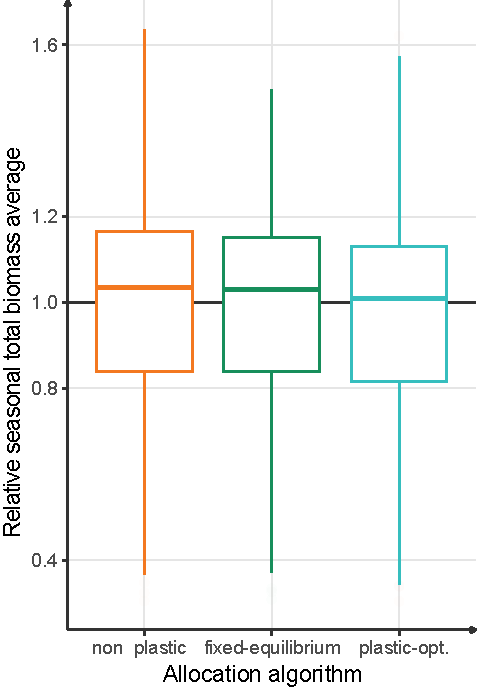
\includegraphics[width = \textwidth]{./2_PP/Figures/Comm/comm_BMtot_differences.pdf}
\caption[Average total biomass in plasticity treatments]{Average total biomass relative to \textit{non plastic} simulations, in the three plasticity treatments.  To negate the variability due to the parameter sets, the variable is divided by the mean value for the\textit{non plastic} treatment for each parameter set.}
\end{marginfigure}

The productivity of the \textit{non plastic}, \textit{fixed-equilibrium} and \textit{plastic-optimisation} allocation algorithm show little differences. The \textit{non plastic} simulations average biomass tend to be a bit higher in certain cases. Like the diversity and density, the normalised yearly average are used to do the comparison, but the average biomass does not show great variations between plasticity, with a higher variability between sites and seasons. \textit{Non plastic} and \textit{fixed-equilibrium} median are quite similar, and the \textit{plastic-optimisation} show lower productivity than the other two algorithms. Both the conserved average plant biomass and the constant plant density lead to a constant community net productivity.

%\paragraph{Community structure}
%
%Because changes in community structure, no changes in density or productivity but, changes in structure, and competition evenness.
%
%\begin{figure}%[tb]
%%    \classiccaptionstyle
%%\sidebysidecaption{0.60\textwidth}{0.3\textwidth}{%
%    \includegraphics[width=1\linewidth]{./2_PP/Figures/Comm/comm_RAC_pl.pdf}%
%%}{%
%  \caption[Rank-Abundance curves fits]{Rank-Abundance curves.}
%  \label{fg:RAC}
%  %}
%\end{figure}



\paragraph{Plasticity: a winning strategy ?}

\begin{marginfigure}\label{fig:tau}
\includegraphics[]{./2_PP/Figures/Comm/comm_tau_differences_exclusive_groups.pdf}
\caption[Plasticity levels in exclusive groups]{Plasticity levels of species that are present in only one type of plastic treatment. Each point represent one distinct species.}
\end{marginfigure}

The allocation algorithm is expected to alter the fitness of potentially plastic plants. The selective effect of the allocation algorithms is investigated by plotting the $\tau$ value of species that are maintained in only one of the algorithms (in figure \ref{fig:tau}). Because of the plasticity cost, the selection of species with low values of $\tau$ signifies an improvement of the fitness due to plasticity. The distribution of $\tau$ is fairly high for \textit{non plastic} species and almost 75\% of the species have a value above 0.8, whereas \textit{fixed-equilibrium} specific species have lower values ranging from 0.2 to 1 with the median arond 0.7 and the \textit{plastic-optimisation} species have even lower values with a median around 0.55.
%Are plastic species more selected than the other ? Probably a bell-shape curves



There is a selective effect of the allocation algorithm on the axis related to the plastic strategy, but the resource-use strategies could also be impacted.

%\section{Strategy}

%\subsection{Results}
\paragraph{Variable strategies}

After the productivity and the diversity, the identity of the communities is investigated.

The mean and median values of the CWM of the resource-use strategies (PAR and PAS) do not show any shift between non plastic and fixed-equilibrium algorithms. The strategy variability is lower for the root strategy, than for the shoot strategy. The variability is relatively high compared to the differences between the two algorithms. The plastic algorithm show low values for the mean and median, with high variability.

Root strategies show high values (around 0.8) of active tissue allocation is all algorithms, in contrast with lower values of the shoot allocation of active tissues (around 0.6).

\begin{table}[]
\centering
\caption[Tissue resource-use strategy at the community level]{Summary statistics (mean, median and standard deviation (SD)) of the community weighted-mean of resource-use strategies in root (PAR) and shoot (PAS) for the three main allocation algorithms.}
\label{table:comm_strat}
\begin{tabular}{l|ccc|ccc}
                      & \multicolumn{3}{c}{PAR} & \multicolumn{3}{c}{PAS} \\
Variable              & Mean  & Median & SD     & Mean   & Median  & SD    \\ \hline
Non plastic           & 0.801 & 0.823  & 0.0733 & 0.644  & 0.657   & 0.152 \\
Fixed-equilibrium     & 0.804 & 0.823  & 0.0714 & 0.653  & 0.657   & 0.143 \\
Plastic\_optimisation & 0.749 & 0.778  & 0.133  & 0.589  & 0.600   & 0.200
\end{tabular}
\end{table}


Unlike the diversity, the identity of the community, defined by the dominating species, does not show a clear shift under plastic allocation. The great variability observed for each algorithm can be easily decomposed and explained because it is linked to the community structure and the dominant species. To decompose this variability in the identity, the community weighted mean 
%Select different strat? meh, from very site specific strats (one dominant species), to more variable within the site, but less differences between the strats. Shift from beta diversity to alpha diversity.
To analyse this variability, the community weighted means (CWMs) for the proportion of active tissues in roots (PAR) is visualised along time for the 6 sites, for 5 representative parameter sets (see figure \ref{fig:comm_strat}. The variability is decomposed between the spatial and the seasonal variability. Under \textit{non plastic} allocation, the CWM values for PAR are stable during time, but contrasted between sites. In contrast, under \textit{fixed-equilibrium} and \textit{plastic-optimisation} allocation, the temporal variability is greater, but the site specific means are closer. This pattern is reproduced for the shoot resource-use strategy (data not shown).


The differences in community structure certainly explain these contrasted source of variability of the community identity. The structure is altered by the increased species richness under plastic allocation (see figure \ref{fg:comm_str}, leading to a reduction of the abundance of the most dominant species, in addition of a long tail of the rank-abundance curves due to numerous species with low abundances.

\begin{marginfigure}%[tb]
%    \classiccaptionstyle
%\sidebysidecaption{0.5\textwidth}{0.4\textwidth}{%
    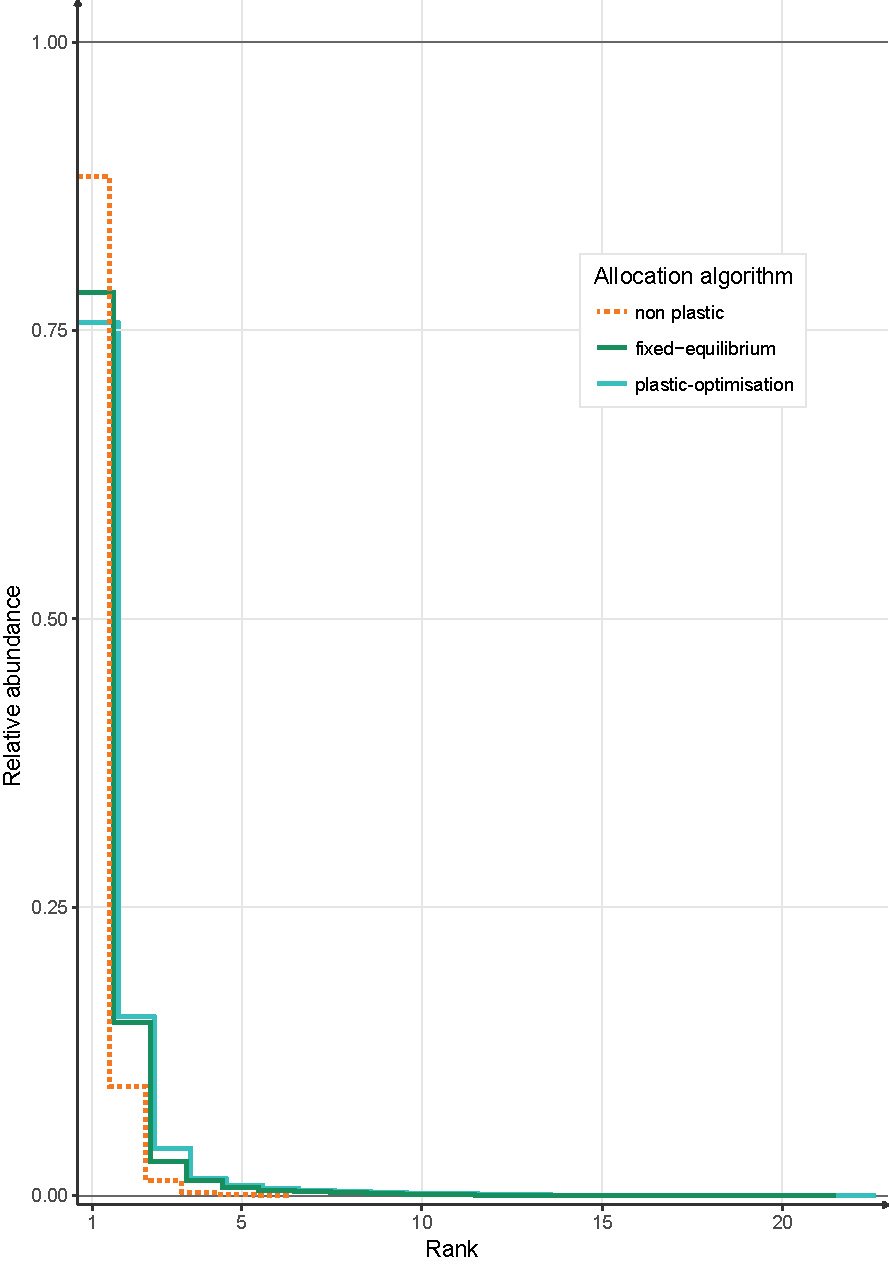
\includegraphics[width=1\linewidth]{./2_PP/Figures/Comm/mean_com_str2.pdf}%
%}{%
  \caption[]{}
  \label{fg:comm_str}
%  }
\end{marginfigure}

This shift in structure at the community scale, but also at the meta-community scale suggest a strong effect of the allocation on the overall structure of the ecosystem.
%Lead to changes in strats? If yes, is it direction\\
%al, or is the direction depends on species?%
%Do species change a lot there strategies?

%Is it always in the same direction for all species ? (reproduce Kichenin).


\begin{figure}%[tb]
%    \classiccaptionstyle
%\sidebysidecaption{0.5\textwidth}{0.4\textwidth}{%
    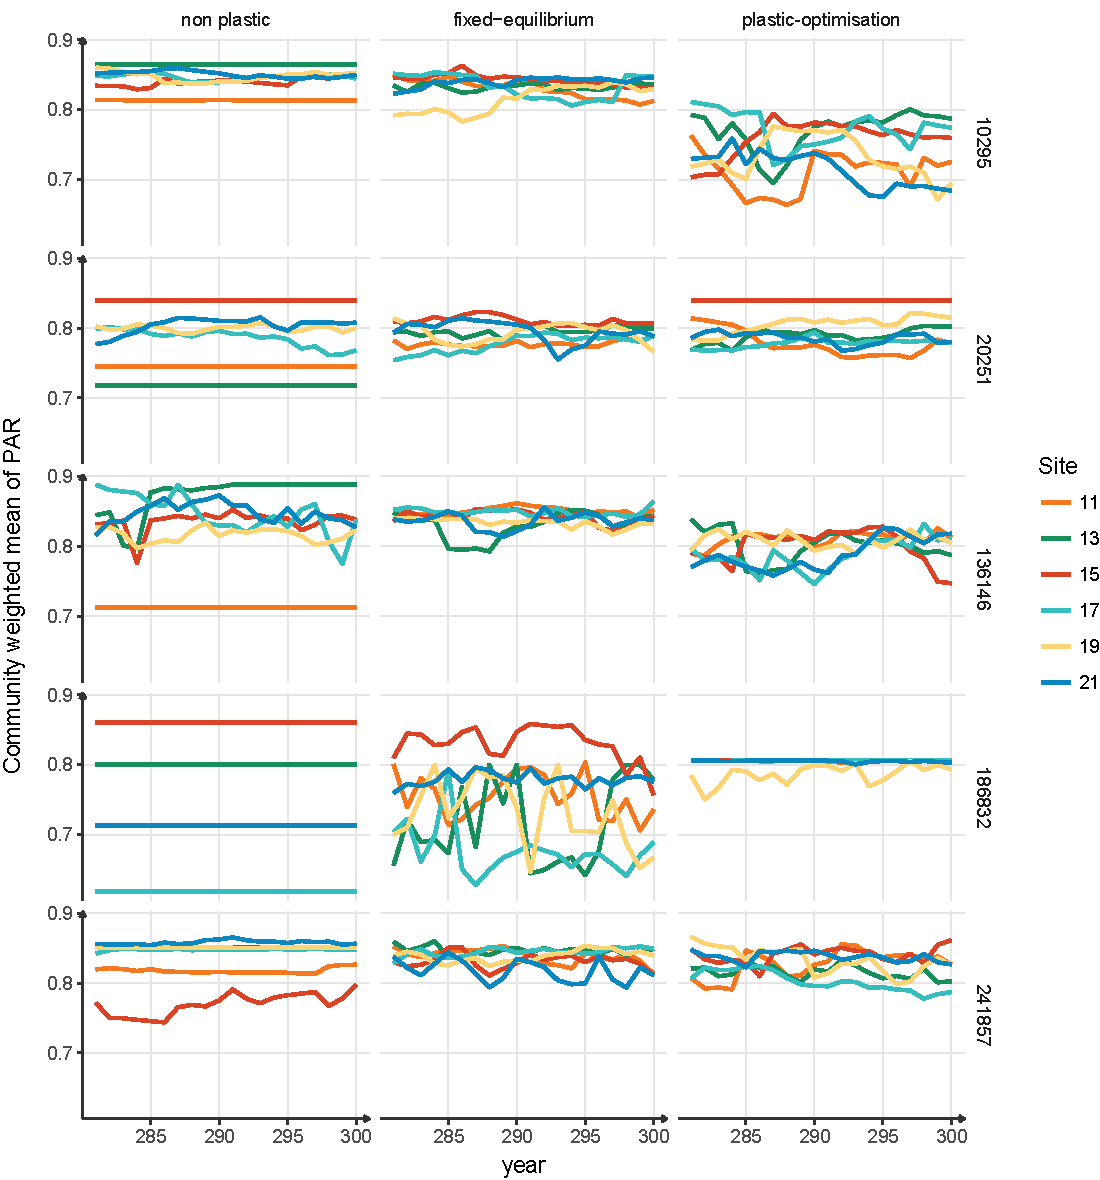
\includegraphics[width=1\linewidth]{./2_PP/Figures/Comm/comm_variability_lines.pdf}%
%}{%
  \caption[Spatial and temporal variability of the CWMs of the PAR]{Community weighted means of the proportion of active tissues in roots for each site, as a function of time and the allocation algorithm, for 5 representative parameter sets.}
  \label{fg:comm_strat}
%  }
\end{figure}


\paragraph{Different diversities}

% shift from beta to alpha diversity
Introducing plasticity in allocation lead to a shift in diversity types. \textit{Non plastic} simulation tend to have more differenciated sites, capture in high values of beta diversity, but with low alpha diversity as previously discussed (see figure \ref{fig:diversities}). 

\begin{figure}\label{fig:diversities}
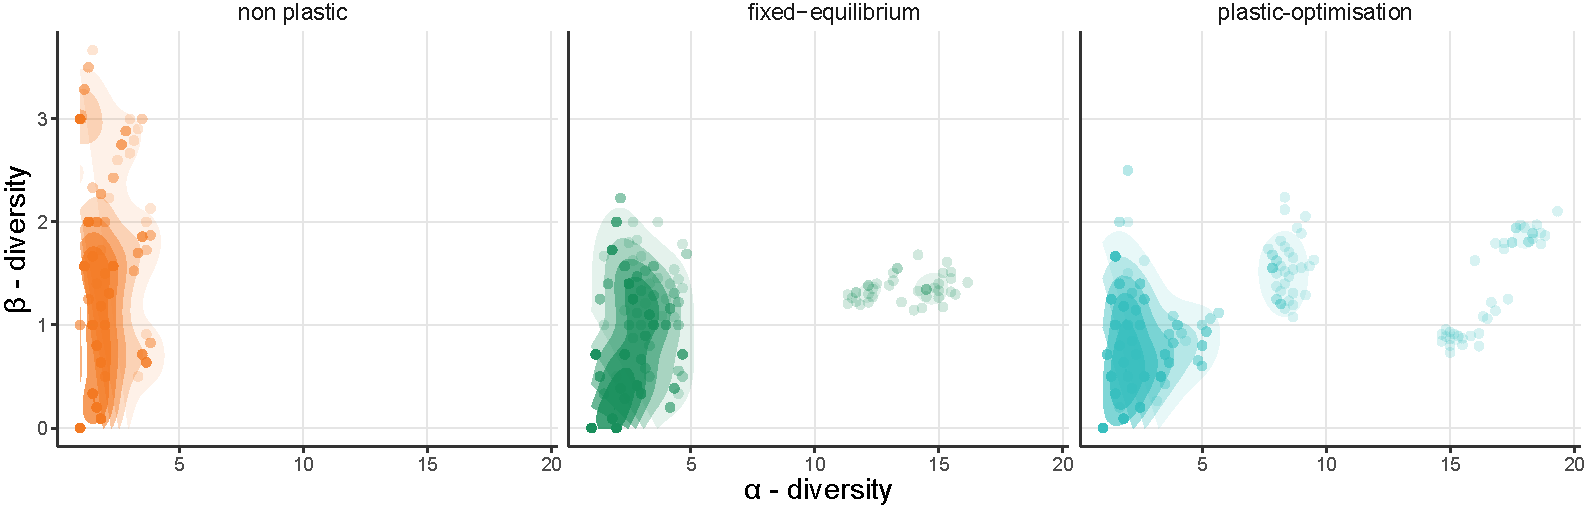
\includegraphics[]{./2_PP/Figures/Comm/comm_div_differences_alpha_beta.pdf}
\caption[Alpha and beta diversities as function of the allocation mechanism.]{Alpha and beta diversities as function of the allocation mechanism.}
\end{figure}

% what about functional diversity?

\subsection{Discussion}

%\paragraph{Competition evenness}

%The plasticity allows the emergence of new phenotypes that are plastic. Leading to higher density in competitors, and greater evenness. Hard to detect because not the same number of species, or require other experiments. 

\paragraph{Filtering} 
The great increase in the species richness observed under plastic allocation, for both the \textit{fixed-equilibrium} and \textit{plastic-optimisation} algorithms,  
results from a reduction of the strength of the filters. The results at the individual level suggest a weakening of the abiotic filter (1) as the importance of the plastic dimensions is reduced (static gain) and (2) variability in conditions can be overcome creating new habitat possibilities (dynamic gain). In the other hand, the reduction of the abiotic filtering was anticipated to increase the competition intensity as more plants can settle in a given habitat.
The overall reduction of filtering suggest a greater importance of the abiotic variables compared to competition as a filtering process. But it is difficult to distinguish the two process in this simulation model as they both are expressed by variations in the water and light availability and are perceived in a similar way by the plants. 

%Specific simulation experiment designs varying the dispersion of the strategies of the invading species could help disentangle these effects.  Detail these experiment and results interpretations

The absence of changes in the plant density, together with the stability of the community productivity, support the idea that if the abiotic filtering is reduced, it goes with an increase in competition. Therefore, the increase in species diversity is explained by a shift from a non uniform abiotic filter, to a more uniform biotic filter. Better understanding of the interactions between species strategies, and how they are modulated by plasticity could help building such interpretations at a higher level based on existing theories \parencite{chesson_mechanisms_2000}. The current implementation of \model contains specific functions dedicated to paired simulations to evaluated these interactions. Determining the transitivity properties of these interaction is also crucial to understand the capacity of the model to maintain stable coexistence \parencite{levine_beyond_2017}.


Alternatively, the plasticity allows species that suffer from changes in resource availability to maintain a positive growth rate during stress periods. Because these plants are maintained, they keep the competition intensity level while this intensity would decrease under \textit{non plastic} allocation where these species disappear. 

With a perspective from coexistence theory could explain the high diversity by the effect of the plasticity as a equalizing mechanism. Allowing species to converge toward better phenotype, or to resist stresses, maintain a certain fitness evenness. While these species are maintain, stabilizing mechanisms such as asymmetric competition can play a bigger role. Indeed, the differences in resource-use strategies suggest a greater intra-specific competition that inter-specific.

Finally, the fact that the species richness is not altered by the cost of the plasticity for \textit{non plastic} simulations (making certain phenotypes non viable), but is altered under plastic allocation, support teh fact that the species richness effect results from the allocation algorithm rather than the plasticity cost.


\paragraph{Productivity \& density}

% same level of prod, low increase in pl: probably sub-opitmum convergence
As mentioned, the productivity is mostly conserved between the allocation algorithms, as the plant density. I hypothesise that the increase in competition compensate the static and dynamic gains provided by the plasticity. It suggests that under \textit{non plastic} allocation, the carrying capacity of the sites is reached. In the other hand, it could be that the increase in competition leads to a decrease in resource-use efficiency as explained by the game theory.

The density of plant is also unchanged. This is consistent with the stability in productivity. This stability in the plant density eliminates any sampling effect that could explain an increase in the observed species number for a given plot area as observed in \cite{lepik_high_2005}.


\paragraph{Community structure}

The increase in the species richness necessarily comes with a change in the community structure under plastic allocation. This shift consist in the reduction of the dominance of the most abundant species, an increase in the second and third dominant species, as well as a longer "tail" with many species of low abundance. While the presence of numerous low abundance species could suggest marginal effects  of the plasticity allowing the maintenance of rare species at the border of their niche, the reduction of the relative abundance differences between the species dominating the community demonstrates a stronger effect. 
%Shift in community structure

This strong effect of the plasticity on the community structure explains the differences in identity variability under the two types of allocation algorithms. In on hand, under the \textit{non plastic} allocation, the identity varies mostly between sites, but stay fairly stable between seasons. In the other hand, the variability in temporal rather than spatial under \textit{fixed-equilibrium} or \textit{plastic-optimisation} allocation. Because the niches are narrow without plasticity, the small climatic differences between the sites lead to different compositions and high spatial heterogeneity in the community identity. The strong filtering force that constitute the changes in conditions does not allow species at low density to establish. These species release the competition intensity when they do not survive climatic stress, offering more resources for the dominating species that translates into a large reproduction effort. Because of storage effect, and strong abiotic filtering, the dominant species is favoured even in bad years. The combination of the sensitity of the fixed phenotypes to changes in conditions with population dynamics favours stable low diversity communities. Under plastic allocation, the niches are wider, allowing more species to invade and survive a given habitat, despite changes in conditions. Because they have wider niches, and the climatic conditions between sites are not that different, the chance that they invade multiple sites are higher than in \textit{non plastic} allocation. Because more species are present, and the competition is more even, the seasonal variations in conditions allow changes in the relative abundance of the species while the community composition is stable. These changes alter the community weighted means and therefore the identity of the community. The differences in species composition and the effects on the CWM of PAR for the three allocation algorithms are illustrated in the figure \ref{fig:explain_strat}.

\begin{figure*}\label{fig:explain_strat}
\includegraphics[]{./2_PP/Figures/Comm/explain_par_variability.png}
\caption[Effect of the community structure on the inter-site variability of the community identity.]{Inter-site and inter-season variability of the community identity (A) explained by the effect of the plasticity on the community structure (B).}
\end{figure*}

%The allocation algorithm, by impacting the niches and the importance of the abiotic filtering, controls the mechanism driving the community structure.

%also, Jung \cite{jung_intraspecific_2014} show contrasting response between species and within species - might not be the best 

\paragraph{Different mechanisms for different diversities}


While many diversity indexes could be used to decompose and analyse the diversity of such communities, these simple indexes (alpha and beta diversity indexes) are sufficient for the level of analysis and they express the differences in the structure of the ecosystem caused by the allocation algorithms.

%why higher alpha div
The increase in alpha diversity has already been discussed and results from a niche widening (or a reduction of the abiotic filtering). The beneficial value of the plasticity to explain this increase in alpha diversity is demonstrated by the significantly lower value of $\tau$ for the species unique to one of the two plastic algorithms for each parameter set. 
% Talk about species TO and tau.

The decrease in beta diversity is explained by the larger overlap between community, caused by a larger overlap between species niches. Such effect could even be reinforced by a different implementation of the link with the meta-community. In this set of simulations, the meta-community is composed of the initial set of species, evenly abundant, where invading seeds are randomly sampled. A different approach could be to consider all sites connected, and sample the invading species from the seeds produced in the other sites. In the case of the \textit{non plastic } allocation, because the sites are highly dominated by one species and the site specific conditions generally do not match the narrow niches of the species, a low number of non adapted seeds would not be able to invade the other sites, and reduce the possibility of coexistence relative to a sampling from a much richer meta-community. This would accentuate the contrast between the alpha and the beta diversity. Under plastic allocation, the community share multiple species, if the seed dispersion is limited to the seed produced within the sites, there would be a large redundancy and a low turn-over in the incoming species (relative to a random sampling from a large meta-community) leading to a very low beta diversity. By affecting the niches and therefore the relative distance between sites in the "niche space", the phenotypic plasticity greatly alters the structure, not only of the communities, but also the meta-community.
%Plasticity allows for bigger niche (variability dimension), more chance to build enough "growth potential" to persist. Otherwise, other species that are dominant, because other species can settle, take advantage of it.
%Should look at the growth rates hierarchy for a couple of simulations.

% but also lower beta


% diversity indexes

% What does it mean to modelling and to community properties ?



\paragraph{Statistics}

The allocation algorithm is only one of factors that impact the response variables that are analysed in the previous sections. The parameter sets and climatic variables (year and sites for community-level simulations) also greatly impact the outcome of the simulation. While the perfect knowledge of the model and the total control over the simulations allow us to decompose and disentangle all these effect, the focus has been on the effects of the allocation algorithm, relative to the other effects. As mentioned in the method, the normalisation relative to the mean of each parameter set eliminates partially the complex effect of the numerous parameters on the scale of the variables, while keeping the overall behaviour (reduction, increase or stability). It also allow to compare the effect of the algorithm relative to the other factors source of variations (season and site). Maybe another normalisation could have been performed (standardisation), but this methods seems to provide already consistent information.

Ones could regret the lack of statistical analysis to estimate the significance of the effects. But, as mentioned the total control and knowledge of the model would allow to ensure significance results for any test, and therefore is not informative (see \cite{white_ecologists_2014} for extended arguments). While the effect size could have been calculated, the graphical representation produced provide enough information to estimate these effect size and compare the effect of the explicative variable of interest (allocation algorithm) to the variability caused by the other factors. 

I believe the representation of the model outputs through specific visualisations gives a better understanding of the general behaviour of the model, as well as an intuition of the unique differences between the different conditions, than large tables and statistical test could do in this context. 
%Interaction between plasticity effects and parameter sets, but the interest here, even if  it is interesting. Higher variance due to site and weather. The almost perfect knowledge of models allows an extremely precise decomposition of the effects, but at the risks of loosing broad effects. The difficulty is to measure the relative strength of these effects, and generalise. But, by essence, the parameters are suspected to have a significant effect that can be identified, otherwise it would not have been included in the model.

% need to reread that, but decomposed when possible, needed, or to show consistency. Not always, to make the description and message clearer.  white_ecologists_2014 : no statistical tests



\paragraph{Plasticity \& community properties}


\paragraph{Robustness}

Is it robust ?


Among the \cite{roscher_contrasting_2015} + jena and diversity (grime ?)

\paragraph{Strategic plasticity}





\subsection{Phenotypic plasticity and global change}

2 perspective: differences between with and wtihout pl. Effect on plastic and on non plastic sp.

% critical transition in non plastic communities

% more stable because more diverse, closer communities

% plasticity : more even competition : larger niche -> smoother transitions

% resistance to stress amplitude and frequency : more heterogeneous comm, either more resistant, or more plastic. until only resistance  less rapid shift in identity because asymmetric dynamic gain



% what about management : abandunment or fertilisation: 
% - abandonnement: less plastic species,  plasticity itself predict smoother transition
% - fertilisation : more exploitative, more plastic, could work better than expected if plasticity is considered.

\paragraph{Measures and rules}

intra-specific variation : jensen inequality : with negative effects on coexistence. 

Jensen's inequality: question of measure.

pl = source of variation: driven. There are causes to this variability. Supposing variability under constant rule does not make sense to me. Variability because non constant rules. Under non constant rules (climate, interaction coeeficients, stochasticity) pl has non linear effect (static gain benefit to non fitting species, or asymmetry in dynamic gain) but mostly favour the diversity.

More genetic approaches for the genetic intra-specific var. effect (not just pl), but I on't think it is negative... at least more lickely to alter the source of vairability or the for mof diversity, as observed here from beta to alpha.

measures and rules

\paragraph{Intra-specific variability}


%
\begin{fullwidth}
This short final chapter summarises the main results and advances produced during this PhD. It is also the opportunity to look ahead and trace future directions to extend upon this work. Imagining extensions to implement and questions to explore is an infinite game, and while many developments are proposed, I try to keep this discussion succinct and close to the current state of the model.
%While researchers are prone to imagine many developments and follow exiting ideas, I try here to be succinct and to consider only a few of the many paths we could follow to extend the model and progress in the field of community ecology.
\end{fullwidth}

%_________________________________________________________________________________
\chapter{Synthesis}
%
%Point out the novelty, acheived work 
%
%begin to fill the gaps of community dynamics: \parencite{berger_competition_2008}: effect on local environment, adaptive behaviour and below-ground.
%
%Pllus: lack of diversity.
\section{A new agent-based model of mountain grasslands}

The implementation of the model \model was the opportunity to develop a new framework from scratch to tackle unresolved scientific questions. Thanks to the freedom that was given to me, I could approach the project in a personal way, establishing the foundation concepts, accumulating ideas, and developing a complex model of grassland communities.

\paragraph{Filling the gap}

The model developed had the ambition to fill the gap between fine-scale agent-based models, integrating physiological processes, fine-scale resource dynamics and phenotypic plasticity with large-scale community dynamics model, long-term dynamics of numerous species in a heterogeneous environment. Filling this gap is necessary to better understand and predict the dynamics of natural (and semi-natural) systems in the context of the global change, affecting both the climatic conditions and the management scenarios. On one hand, computaional cost and design choices limit our ability to deploy fine-scale models at large-scales to integrate the effects expressed at the local-scales. On the other hand, the large-scale community dynamic models overlooked some fine-scale processes such as the intra-specific variability, and in particular the phenotypic plasticity. Better integrating these two levels can help us better predict changes in the main properties of the grassland communities, and the effect on the ecosystem services.

\model manages to fill this gap by integrating the plant functioning and the phenotypic plasticity into a framework based on the leaf economic spectrum and developed around strategic allocation trade-offs. The partitioned allocation to the active and structural tissues regulates the balance between resource exchanges and respiration and tissue turn-over costs. These trade-offs enable a coherent representation of the plant functioning while drawing a closed strategy space where the diversity of plant species can be modelled. This strategy space, which is at the core of the model, is also at the centre of the phenotypic plasticity conceptual framework developed in this work. The phenotypic axes drawn by the trade-off offers a space in which plant can evolve\sidenote{not in an evolutionary perspective.} based on their projection of the external conditions. This projection is the engine that drives the phenotypic plasticity and allows the modelling of a strategic plasticity, that contrasts with ubiquitous plasticity. The implementation of multiple rules to drive this plasticity allows a comprehensive understanding of this mechanism of phenotypic plasticity and to test the robustness of the observed patterns.


\paragraph{Consistency}

While the steps of parametrisation highlight some progress to make in the implementation of the phenotypic plasticity, the current version of \model offers stable growth patterns, both at the individual level and the community level, and a strong tool to start exploring the effect of the phenotypic plasticity. This stability is supported by the consistency of the results between the numerous parameter sets observed. Despite the difficulty to reproduce some specific empirical patterns, the plasticity improves the performance of the model and impacts its behaviour, encouraging us to further explore its effects at the individual scale first, then at the community scale.

\paragraph{Strategies and performances}

The strategy space built with independent strategy axes allows the modelling of a multitude of species. While the diversity offered by this new framework is not fully explored and used, the vegetative dimensions are extensively analysed. Because there are based on strong empirical trade-off, these dimensions draw a wide performance landscape that (1) have the potential for high functional richness, and (2) evolve as a function of the resource levels. Establishing a link between this landscape with the plasticity mechanisms will be key to better represent the phenotypic plasticity. This analysis also identifies the root mass fraction (RMF) dimension as a key trait to control the plants' performances, and therefore support the investigation of this axis as a plastic dimension.


\section{A better understanding of the effects of plasticity}

The multiple plastic allocation algorithms, with varying plastic dimensions (RMF only, or in combination with the proportion of active tissues) and two alternative driving rules (maintenance of the equilibrium or growth optimisation), let us explore the potential effects of the plasticity. At the individual-scale the effects on growth and surviving are analysed, and at the community-level the realised impacts on communities' properties are studied with plot simulations.

\paragraph{Niches and gains}

At the individual level, the main effects of the plasticity are captured by the widening of the potential niche and the reduction of the fitness differences. These modifications of the niche are explained by two main mechanisms: (1) the static gain in fixed conditions allows the convergence of plant individual phenotype to an optimum phenotype, this levels the competition but does not affect the maximum growth. This convergence reveals a trade-off between the species and functional diversities. (2) the dynamic gain, in variable conditions, enables the plastic plants to adapt their phenotypes over time, and increase the maximum growth rate relative to the non plastic allocation maximum growth. This type of plasticity mostly favours exploitative species that would suffer more from resource variability under non plastic allocation. This effect could greatly affect predictions of the dominant species under climate change scenarios. While this gain also induces some convergence, and therefore a similar trade-off between the species and the functional diversity, it offers more potential for higher functional diversity, especially if the plasticity has a physiological cost.

The phenotypic plasticity can have contradictory effects on the coexistence mechanisms, by the reduction of the fitness differences on one hand and the reduction of the niche differences, on the other hand. This paradox can be resolved by community-level simulation experiments. These experiments are also the opportunity to test the strength of the plasticity effects on the productivity and the community identity.

\paragraph{Integration at higher level}

A simple parameter filtering step ensures the stability of the community level simulations but does not offer enough information to disentangle the intricate effects of the multiple parameters. 

The community-scale simulation experiments, over multiple seasons and sites, reveal a strong driving influence of the daily weather on the productivity. Despite a strong potential effect of the plasticity on the individual growth, the cumulative growth is not strongly improved under plastic allocation. These results suggest a limitation by the carrying capacity of the conditions, and an increase in the competition intensity to compensate for the reduction of the abiotic filtering. Indeed, the niche widening gices more species the opportunity to invade a habitat by reducing the abiotic filtering. But the expected stronger biotic filtering effect of an increased competition is negated by the reduction of the fitness differences between the coexisting species. The positive effect of the plasticity is demonstrated by the invasion of species with higher plasticity ability.


\paragraph{Different diversities \& structures}
This cumulative effect of the reduction of the abiotic filtering and the reduction of the fitness differences leads to changes in the community and meta-community structure. Under plastic allocation, the abundance of the most dominant species is reduced, and numerous species are able to reproduce at low abundance. This shift in the community structure, from a mono-specific or highly dominated community to a diverse community, goes with an increase in alpha diversity. But, the larger number of species within one site also translates to a greater overlap in species distribution between sites. The sites show more distinct communities under non plastic allocation. The plasticity favours the alpha diversity, while non plastic allocation better distinguishes the different sites because of more narrow and distinct niches.

The alteration of the community and meta-community structures also affect the identity of the system and leads to less distinct community strategies and more variable identity over time. This effect can greatly affect the overall dynamics under climate change, with progressive changes in the abundance and the dominating strategy under plastic allocation, but rapid shifts in dominance under non plastic allocation, disturbing the meta-community dynamics.


\paragraph{Further exploration}

The identification of clear mechanisms due to the phenotypic plasticity that affects the community dynamics pushes to explore more in details the questions around these dynamics, especially in the context of the climate change. Moreover, the framework developed, based on the projection of external conditions and multiple allocation rules, does not completely solve the problem of the conceptualisation and implementation of the mechanism of the phenotypic plasticity. Further work needs to be done, but this model offers a great basis and a reference point for future implementations. It also opens the door to approaches that link the community dynamics with an epigenetic and genetic transmission of the information. These questions are further developed and discussed in the following section.

% and new questions


%
%%\section{Phenotypic plasticity: the individual response alter}
%\section{Modelling diverse community}
%
%It grows.
%
%It's diverse.
%
%It's stable.
%
%It's driver dependant? (at least at individual level.
%
%
%\section{Effect of plasticity of mountain grasslands properties}
%
%Did a bit what I accused other model to do: have a discrete conception of plasticity. However, the results at the community scale are encouraging and demonstrate the interest of such approach.
%%
%%\paragraph{Interpretation}
%%In modelling studies it is necessary to realised that we are not looking at the real system, but rather comparing models. Therefore, when we look at the results of model including or not plasticity, if we are looking at the direct effect on the model, outcome change, while there do not change in reality. So the interpretations of the effects on the model behaviour must be translated, not as effects on real the community, but as effects on how we understand the processes shape this community. An increase in individual growth rate due to plasticity is consequently translated in "we overestimate growth parameters in non palstic growth models".  Not sure it is that interesting. Maybe talk about the weight between processes, rather than parameters that are calibrated and are less linked to the understanding of the system.
%\subsection{Identity}
%\subsection{Productivity}
%\subsection{Diversity}
%
%\section{On plasticity modelling}
%One strong assumption this modelling relied on was the existence of a strong link between fitness and environnemental condition. This is has been proven to be partially true as \model was able to express improvements in fitness thanks to plasticity. However, in some situations, the plasticity leads to reduction in fitness, or eventually to complete phenotypic dead-end. The temporal dimension of plant growth, and the difficulty to capture that makes this assumption hard to maintain in such complex systems with strong dyunamics. Moreover, such assumption do not necesserally take into account competitive behaviours better capture by game theory and other modelling approaches \cite{farrior_resource_2011, dybzinski_evolutionarily_2011}.
%
%
%\subsection{How to make it work better, with what consequences} 
%\paragraph{On memory}
%
%Despite talking about molecular basis of the plasticity, did not really make use of this knowledge. Should better use biological idea (even if a bit more complex). Especially for memory and recovery: idea of stress, memory and loss of memory (recover) to avoid maladaptive responses \parencite{crisp_reconsidering_2016} ! ! ! 
%seee also cues reliability \parencite{simons_playing_2014} and \parencite{scheiner_genetics_1989, scheiner_genetics_2002, scheiner_genetics_2012, scheiner_genetics_2013}
%
%\paragraph{On plastic traits}
%
%Non composite traits (here SLA plastic only because of density, but does not consider thickness plasticity).
%
%\paragraph{On drivers}
%
%Fitness proxy ? yeah \cite{ryser_consequences_2000} resource use optim by pl, but \cite{franklin_modeling_2012} too variable ... stess response oriented. 
%
%
%Nitrogen instead of water, leaves do not respond to water changes (unless low nitrogen becaue water limitation is more nitrogen limitation really \parencite{farrior_competitive_2014}), does not work well with integrative vision to ignore nitrogen.
%
%
%It's not only about optimum, but also vulnerability and error. 
%
%\subsection{Genericity and extensions}
%
%About extensions, but the process, despite failing completly capture real growth dynamics (but we already disccused why), built the fundations for resistance-risk plasticity with accumulation of risk cues, extend risk avoidance - resistance trade-off (similar than droudgt see \cite{kooyers_evolution_2015}?) for herbivory.
%
%\section{The limit of the species.}
%
%Refer to the litterature review part.
%
%In this work, but also because of the improvement of molecular biology, and the deeper and deeper dive ecology is doing within individual, the limits of species are fuzzy (started with trait and the introduction of continuity). At some point, there will be a need for a way to go back from the a space of numerous continuous dimensions to the species. Also, understanding species as evolving 3D objects, where the different aspects of intra-specific variations play different shaping roles.
%

%_________________________________________________________________________________
\chapter{Outlook}

This section explores further developments of the model. The first section focuses on how the phenotypic plasticity is modelled, and how alternative approaches can help understand this process and its effects. The second part of this discussion describes ways to widen the scope of the model by taking advantage of the already existing resources.

\section{How to model phenotypic plasticity? }

The framework developed during this project constitutes a step forward in the modelling of the phenotypic plasticity. It integrates the idea of streategic plasticity \parencite{bradshaw_evolutionary_1965, dewitt_expanding_2016} within a phenotypic space drawn by allocation trade-offs that allows the modelling of diverse community. But the limitations shown by the current implementation reveals that the question of the modelling of the phenotypic plasticity is not resolved. While the question of the plastic dimension will always be present when modelling phenotypic plasticity, the main interrogations revolves around the drivers and the use of the information. 

%how do we think about plasiticity: this model is a step forward, despite seen as a ...

\paragraph{Explore the limits}

The question of the plasticity as a strategy trait was not fully explored despite being a centre point in the design of the model. This plasticity as a strategy, rather than a growing function, expresses the idea the existence of limits that justify that not all species are plastic \parencite{dewitt_costs_1998 ,  van_kleunen_constraints_2005, valladares_ecological_2007, auld_re-evaluationg_2009}. These plastic, in addition to be observed in natural systems, are also needed in the context of the model to avoid convergence and Darwinian demons. These limits are numerous and can be separated in multiple categories: actual limits that prevent an effective plasticity that increases reliably the fitness, and costs that negate the fitness gain provide by the changes in phenotype.\cite{valladares_ecological_2007} also distinguish internal limits and ecological limits, but these are not always clearly circumscribed and quantified. The internal costs must be implemented in the model, to avoid unnatural behaviours and explore emergent properties. The ecological limits, on the other hand should emerge from the mechanisms implemented. For example, the variability of the climatic conditions, should favour the selection or species with high plasticity in the current implementation of the model, if it is not too variable and impredictable. This could be tested with simulations with two axes of treatment: temporal variability and auto-correlation. Mechanistic approaches, informed by the knowledge of the plant biology, allow the consideration of internal limits such as morphological limits \parencite{valladares_ecological_2007}, as implemented in \cite{maire_plasticity_2013} or \cite{lohier_analyse_2016}, and to a lower extend by the allocation trade-off in \model . But as observed in this implementation, the allocation trade-off does not take into account the whole extent of the morphological limits, and further work is needed to quantify those. The mechanistic model also prevent unrealistic plasticity by the natural limitation of the phenotype's flexibility \parencite{forsman_rethinking_2014}. The balance between the growth and the turn-over must be finely calibrated to capture this limitation of the plasticity that can cause lags in the plastic responses \parencite{dewitt_costs_1998}. % calibration ! ! !
 Other cost costs are harder to quantify, such as the maintenance, acquisition and production costs. Methodologies are proposed to study the potential cost of plasticity \parencite{dewitt_costs_1998, valladares_quantitative_2006}, they have found limited effects in natural systems \parencite{van_kleunen_constraints_2005}, despite potential effects in a context of low genetic variation \parencite{dechaine_constraints_2007}. The difficulty to quantify globally the plasticity cost comes from the difficulty to disentangle the different forms of cost \parencite{murren_constraints_2015}, the potential cost of homoeostasis \parencite{van_kleunen_progress_2007}  and statistical limitations \parencite{auld_measuring_2011}. These difficulties are illustrated by the implementation of the cost of the plasticity in \model . The production cost, relative to the expression of an alternative phenotype different from the current phenotype, can intuitively be expressed as a function of the phenotypic distance between the two phenotypes \cite{valladares_quantitative_2006}. But the choices relative to the computation of this distance are numerous and hard to justify: should the current or the 'default' phenotype be the point of references, what axes are considered (composite traits such as the  SLA, individual traits, morphological or chemical traits) and their relative importance, etc...
The quantification of the costs of plasticity represents a challenge that requires progress and collaboration from the empirical studies, modelling approaches and statistical method. This challenge is crucial for the quantitative estimation of the importance of the plasticity on the community dynamics.
  % The value of a model like \model resides in its capacity to run simulations to test the validity of these hypotheses. 
%
%The limit of the predictability, variability and uncertainty
%
%The reliability of the external cues about the future stress is a limit often identified.  This uncertainty can ban on factor that explains the failure of the \textit{plastic-optimisation} algorithm to consistently increase plant fitness. The error in the projection of realised conditions (because of unreliable cues, wrong driving rule, or competition interactions)   % non symetry in the fitness landscape, benefit risk, optimum and stability.
%
%Between optimisation and stability
%
%competition % requires better knowledge of how interactions work there , with approaches similar to tilman, and see how plasticity can affect them (
%
%and other traits 

\paragraph{A molecular-inspired plasticity}

As mentioned, having a modelling approach closer to the molecular mechanisms would explicit some internal limits of the plasticity. In particular, the use of reaction norms would capture the complexity of the mechanism and the difficulty to integrate multiple signals. The prediction capacity would also be limited by the form of these reaction norms. It also implies a high number of species specific parameters, increasing with the number of stresses considered. These arguments were invoked to justify the integrative approach of the model, but make the mechanism more grounded in the reality.

The advantages provided by a molecular-inspired approach go beyond the explicit limitations. Species specific reaction norms would at the same allow more amplitude in the plasticity responses, but also more diversity \parencite{kichenin_contrasting_2013, wellstein_intraspecific_2013}. This method could easily model contrasted responses between avoidance and tolerance as a function of the global plant strategy, \parencite{perez-ramos_tradeoffs_2013} or the available information \parencite{heger_light_2016}. This diversity in response also allows responses outside the trade-offs. Despite evidences of an economic spectrum at the intra-specific scale \parencite{hu_novel_2015, fajardo_intraspecific_2018}, the leaf economic spectrum does not totally control intra-specific variations \parencite{fajardo_intraspecific_2018} and plastic responses do not have the same objectives \parencite{ryser_consequences_2000}. Molecular approaches should still be constrained by morphological and physiological limits, but not necessarily the same that determine the default plant strategies.

% about memory
A molecular-inspired plasticity, could better mimic the accumulation of stress molecules, that increase the amplitude of the plastic response following a second stress signal \cite{crisp_reconsidering_2016}. This type of mechanisms also greatly illustrates the idea of species memroy against the plant experience \sidenote{or \textit{memory} as named in \cite{crisp_reconsidering_2016}, but \textit{experience}is prefered here to avoid ambiguity.}. The idea of stress levels, competing with the growth \cite{herms_dilemma_1992} and eventually other forms of stress (frost, grazing, drought , etc...), was originally planed for the model, but the number of stresses were limited to avoid a too complex model. This limitation to resource-related stresses also allowed the simplication of the plastic driving mechanism with the use of an integrative function. But this idea of competing stresses, based on melcular-inspired plasticity and plant-specific experience is attractive and should unlock a better understanding of the plasticity mechanisms.

%more molecular approach, to have stronger patterns, and avoid observed limitations

%break the trade-offs, not the same mechanisms (information, time sale, objectives)
%avoidance and resistance : variability in response.

\paragraph{Plasticity, epigenetics \& genetics}

The framework developed during this work establishes the plasticity as a strategy, but also includes the perception of external conditions as components of the overall strategy. These driving external conditions change at the scale of the season, justifying phenotypic plasticity, but also follow larger trends between seasons. These trends can lead to a gap between the default phenotype, or species memory of the external conditions \sidenote{as tthe two are linked in the model. Here I use these two terms to identify the species stratgy expressed by the default phenotype, but depending on the species memory for the external conditions.}, and the average optimum phenotype, or average experience conditions. This gap can be captured by plants, even in the context of an adaptive phenotype, by the comparison of either the experienced conditions, the stress levels and direction or the plastic responses, to respectively the species memory, the absence of stress or the average phenotype. The quantitative perception of this gap, expressed by directed plastic responses, can be transmitted to following generation to better fit to the general trend in the external drivers. This form of heritability ban have a great effect on the community dynamics, particularly on their ability to cope with climate change. The heritability in intra-specific variable traits provides resilience to environmental disturbances and stabilise trait patterns \cite{barabas_effect_2016}.

The heritability of driven changes in phenotypes also makes sense in a molecular perspective. Indeed, a lot of plasticity mechanisms involve epigenetic inheritable mechanisms, such as histone modifications, DNA methylation or sequence modification \cite{nicotra_plant_2010}.

% genetics and plasticity as a genetic traits that can be altered.
The heritability of driven changes in phenotypes, or driving traits such as the species memory, differ from random mutation and selection. However, the evolutionary process of mutation and selection of traits could lead to a greater understanding of the plasticity processes. First, it would allow the comparison between the dynamics of genetic and epigenetic modifications, and their relative impact on the community dynamics. If genetic modifications can lead to a diversification of the community, epigenetic modifications certainly increases the resilience to rapid environmental shift. Second, the incorporation of genetic algorithm would allow the selection of effective forms of plasticity, especially if the plastic responses are determined by reaction norms with species-specific parameters. The selection of the reaction norm forms, and the study of the species specific parameter distribution can greatly improve our understanding of this mechanisms.

The coexistence of epigenetic and genetic control can lead to particular phenotypic distribution. It may be important to consider such distributions to understand plasticity strategies at the scale of the species \parencite{dewitt_expanding_2016}.


\begin{figure}%[tb]
%    \classiccaptionstyle
%\sidebysidecaption{0.5\textwidth}{0.4\textwidth}{%
    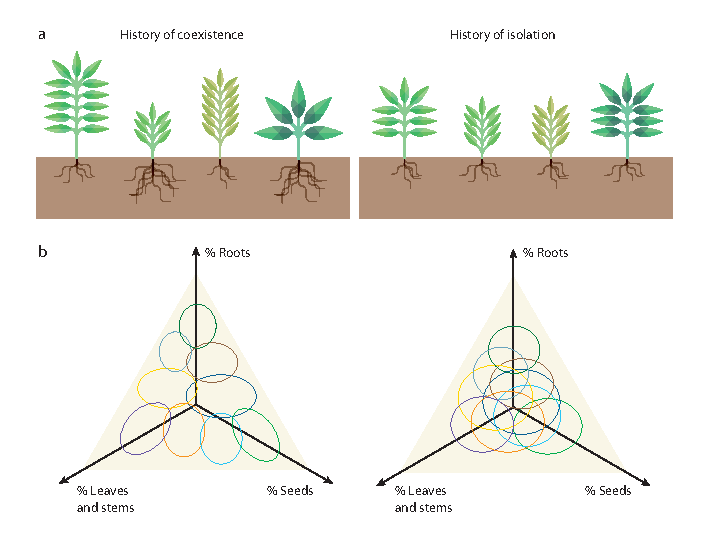
\includegraphics[width=1\linewidth]{./3_Synthesis/graphics/niche_shift.pdf}%
%}{
  \caption[ Evolutionary niche shifts.]{ Evolutionary niche shifts. a) \cite{zuppinger-dingley_selection_2014} find that, when plant species are grown in a common environment, those that have a history of selection in diverse communities develop greater differences in traits than species that have a history of isolation. b) This idea feeds into our understanding of how evolutionary history influences the ecological interactions of species that compete for growth factors such as soil nutrients, light and space. All species face trade-offs. For instance, biomass that is allocated to obtaining soil nutrients (roots) cannot be used to obtain light (leaves and stems) or to disperse to open sites (seeds). Graphically depicted, the resulting ‘trade-off surface’ (triangles) represents all possible ways in which plant species (ellipses) can allocate their biomass. A history of selection in diverse communities results in greater interspecific differences (less overlap of
ellipses) and more specialization (smaller ellipses) than a history of isolation. From \cite{tilman_diversity_2014}, reproduced with the permission of Springer, license number: 	
4386020602501.}
  \label{fig:niche_shift}
% }
\end{figure}

The epigenetic changes, that link the experience of the external conditions with species strategies and transmits this information to following generations may play an important role in the character displacement observed in empirical experiments \parencite{zuppinger-dingley_selection_2014}. The ability of coexisting species to express contrasted phenotypes increasing the biodiversity may rely on the phenotypic plasticity\parencite{roscher_contrasting_2015}, but epignetic processes may play a role in the stability of this mechanisms and a long-time effect on biodiversity \parencite{tilman_density_2014}.



% heritaibility and effects

% link with molecular level mechanisms nicotra and 
%
%The previously mentioned concept of an individual experience competing with a 
%Plasticity as a strategy: genetic dyn + extend the discussion of the limits
%
%heritability: how can it be transfert, wht should be transferred, effect of this heritability (dewiit and barabas)

\paragraph{It is about information}

The development of the implementation of the phenotypic plasticity listed above introduce a lot of complexity and computational costs. Another approach, at the conceptual end of the modelling approaches, is to consider the external resources and stresses as information to solve an investment problem. Once the gains and cost function established, the reliability of the information, the uncertainty and the risks can be computed similarly as in other systems such as economic optimisation problems. This would extend the view of the plant physiology as an economic problem \parencite{westoby_time_2000, wright_worldwide_2004, mcmurtrie_leaf-trait_2011}. Such approach relies on two sides: an explicit and precise description of cost and gain functions, and a prediction of the controlling variables. The former is relies on a good understanding of plant physiology, and current knowledges allow a good representation of these processes, but the costs of the plasticity need to be better quantified as already highlighted. The reliability of the information for the prediction of the future conditions has already been pointed out in multiple studies \parencite{ dewitt_costs_1998, auld_re-evaluating_2009, richter_phenotypic_2012}. The inability of a plant to consider the cost of being wrong is one argument explaining the low performances observed in \textit{plastic-optimisation} simulations, despite a more flexible plastic allocation allowing for a better exploration of the phenotypic space. The productive, but less efficient phenotypes selected by this algorithm do not authorise errors in the prediction of the resource availability because of their higher sensitive to unbalanced organ activities. This particular case could be solved by the evaluation of alternative projection at the same time multiple phenotypes are evaluated. While it would increase the computational cost by increasing the dimension of the space explore, better implementation and exploration algorithm could compensate for this downside. In addition, the overall complexity of the model would almost stay the same as it would require only one additional model to weighted the chance to optimise the fitness with the risk of unstable phenotypes in case of uncertain prediction.

More advanced learning processes can be investigated to model the phenotypic plasticity. The concept of adaptive learning is also a path to explore for the development of the phenotypic plasticity. As genetic algorithm evaluate the success of a strategy by a fitness function at the end of a cycle, individuals could evaluate the performance of plastic response strategies after a few days. The driver of the plasticity resides in the evaluation of the current phenotype for the current and future conditions, in order to eventually develop alternative phenotypes if the performance in not satisfactory\sidenote{this sound finalist, but I use this formulation to emphasise the step of the evaluation of the phenotype. This evaluation can take the form of a concentration in a certain stress molecule in a less perspective approach.}. Therefore, in the context of plastic phenotype, the evaluation step quantifies at the same time the success\sidenote{any relevant fitness proxy.} of the current phenotype, but also the success of the plasticity that lead to this phenotype. The plastic strategy is evaluate through the improvement in the phenotype's success, rather than the absolute value of the fitness function. This relative change in fitness must also consider the external stress intensity to avoid penalising well performing plastic strategies under more intense stress. This evaluation of the plasticity strategy allows to adapt the parameters of the plastic response itself, but also the variables required to build the need projection of condition, increasing the confidence and reducing the risks of the uncertainty mentioned above. This approach however makes sense under a complex and performing prediction algorithm, and may not fit the scope of the current model that focuses on community dynamics. Specific deigns of plastic plant models will be required to explore this track.

%alternative approach: prediction and the information available

%adaptive learning

%stress also informs on how 


\section{Beyond the simple community}

The previous part of the perspectives that emerge form this work focuses on improvements of the implementation of the phenotypic plasticity. But the model already offers a new tool to explore the effects of the phenotypic plasticity on grassland communities that have only been scratched.

\paragraph{The role of the climate}

take advantage of the already present information,
build a better calibration -> more precise, prediction

consider the already implemented feature: frost stress and grazing/cutting.

\paragraph{About ecosystem services}

with better calibration, better quantification of measure traits (that were a bit put on the side here) and more specific results (site and weather)

Link the properties together

\paragraph{The meta-community dynamics}

Can have a pretty good role: reinforce or mitigate patterns 
already possible

landscape dynamics

invasion and critical transitions

\paragraph{The climate change}

precise, calibrated model, closer to real systems to link to ES, with proper landscape dyns.

management scenarios and climate scenarios, intreracton \cite{deleglise_drought-induced_2015}

fantasised view of the model but this exitment makes us work.

%Further reading, thinking and rambling about what's developped in the papers.
%
%%\section{Plasticity and resistance to climatic events}
%
%%\section{•}
%
%\subsection{Better calibration}
%
%Better implementation rcpp or data table struture, plasticity mech, to allow bayesian and pattern-oriented calibration. A lot of species and a lot of parameters. Difficult exercice. But strategies should be limited by functions and trade-off, just need to calibrate shared (process related) parameters and not species specific (strategic) paramters. This is what allows the modelling of diverse community. 
%
%
%\section{Competition and feedback}
%This document focuses on how the plant are doing with the given resources (arrow in fig in margin). However, a key element in competition and resource dynamics (point that separate Tilman appraoches from Chesson) is the impact of plant on resource (fig in margin). Both are fundamental for the understanding on plant interactions, and I argue that understanding the former is necessary to understand the later and have a global view on plant competitive interactions on resources. blablabla competition experiments, resistance to resource shortening (Tilman) and relative homogeneity of resource (homogeneous in influx, content, starting pool, ... ?). Using the term homogeneous allows to use fixed terms and processes, while to me there is a ambiguity around competition that can be seen as: (1) the impact on growth, (2) the winner out of a competitive scenario (with resource shortening). In this later case, the approach of part 4 (?) has limited interpretation since they are not competing. We can intuiitively imagine (from our understanding of model's functioning) that  there is a hierarchical effect on growth, but that is probably reversed in case of (1) shared resource pool (big plant may have access to bigger resource pool in open environment), (2) sufficiently quick resource shortening to lead to death events.\\
%
%in margin: figure resource and interaction.\\
%figure competition decomposition of fitness (growth and survival), and growth related to resource pool (try to have graph approach).
%
%competition change vegetation response to climate change \parencite{van_loon_how_2014}
%
%transitivity and competition \cite{levine_beyond_2017} Could it emerge from the current implementation of \model ? Is it stable with plasticity ?
%
%
%\section{Extend to climate change effects}
%
%How plasticity actually affect the effects of climate change: mitigate or amplify, risk of critical transition.
%
%drought resistance experiments to be done.
%
%Higher diversity: higher risk of invasion?
%
%Take advantage of simulated scenarios of climate change.
%
%\section{Going forward: epigenetic and heritability}
%
%fundamental knwowledge 
%
%effect of heritability and genetic effects (evolutionary perspective) Bring the two perspective together. \cite{scheiner_genetics_1989}
%
%Bayesian model of dev. \cite{stamps_bayesian_2016} Talked about the difficulty to match reaction norms with systemic plasticity: evolutionay bayesian approach to species specific reaction norms.
%
%Epigenetic variation creates potential for evolution of plant phenotypic plasticity \cite{zhang_epigenetic_2013}
%See also \cite{dewitt_expanding_2016} for higher moment of reaction norms controlled by genes
%
\chapter{Extensions}
\fwnewthought{This section is meant to include thoughts and ideas on how to extend \model but that could not be included in the first versions of the model for various reasons. Despite not being included, these extensions are interesting from a scientific or technical point of view, and I hope these notes can be useful to anyone interested in \model or individual based vegetation modelling.}


%\section{Notes}
%
%\subsection{On modelling}
%Frustration: often look obvious, at least it's just logical, there is what we put in...\\
%
%Modelling approach, when not for prediction, what is it about ?
%\begin{itemize}
%\item building understanding
%\item weight mechanisms
%\item test hypothesis
%\end{itemize}
%\

%_________________________________________________________________________________
%\section{Include nitrogen: source of trade-off} %<-- may need to be turned into sections

As seen previously in chapter %\ref{\chapter:trade-of}
, the emergence of trade-off in growth strategy in the actual framework actually rely on a strong genetic constraint over plant plasticity. Indeed, without plasticity cost and low reactivity there would be a high rate of phenotypic convergence of individuals from different species. This is explained by the existence of optimum carbon partitioning (for a given size) in a stable environment. The coexistence of different resource use strategies (exploitative vs conservative) is allowed only through temporal variations and non equilibrium state. This is quite common since a lot of models will predict rapid dominance of one entity in case of equilibrium (need references here).\\
Multiple questions arise from this observation: are the conclusions of this work still interesting in the understanding of the coexistence mechanisms? (I hope I did convince you in the dedicated part of this document, see .. for more details), is it possible to see coexistence of multiple strategies in a temporally stable environment? how can we produce trade-off by including only one more resource?\\

In the following paragraphs I try to answer these questions with theoretical arguments and suggestions on how to integrate them in \model.

%\section{Stable coexistence: the need for a resource dependent tissue efficiency}

Coexistence mechanisms are listed and detailed in the introduction of this thesis (see chapter \ref{chapter:coexistence}). Here I focus on the efficiency of tissues... Nitrogen based, why coexistence ? different phenotype correspond to different limiting resources and for different resource availabilities, different phenotype will optimize the return cost of tissues.Nitrogen also allow the model to have an extra dimension into strategy: WUE (local scale) versus NUE (global scale) (element of reflexion in Maire's thesis).\\
Its also can be related to


%__________________________________________________________________________________
%\section{Specific resistance carbon pools: diversify strategies (and memory)}

Original idea was to have specific carbon pools for different function, and weight the relative allocation based on gain projections.\\

\subsection{Resistance carbon pools}

\section{For more interaction}

This model, thanks to paired simulations should be used to explore the effect of plasticity on interactions and competition.\\
Understanding impact of plasticity on fundamental interaction could nourish the theoretical work on coexistence by linking mechanistic model observations and understanding with more abstract work on the basis of coexistence.

%\chapter{Land-use: a important driver}
%
%\section{Proto-model of management}
%
%Mapping, digestibility and selectivity (smoothing). Grazing and mowing. Height correction.
%
%\section{Individual and collective response}
%Response could be to grow thinner, more fragile leaves to go back on tracks (and take advantages of nutrients and lower competition) or grow bigger leaves and invest in predation resistance/avoidance.
%
%\section{Remaining questions}
%
%Calibration of herbivory pressure.


%__________________________________________________________________________________
%\section{Local adaptation and epigenetic: between species and individual memory}



%__________________________________________________________________________________



%% avoid page break before chapter:
%\usepackage{etoolbox}
%\patchcmd{\chapter}{\if@openright\cleardoublepage\else\clearpage\fi}{}{}{}

\makeatletter %keeps latex from stumbling over @ signs
\renewcommand\chapter{\thispagestyle{plain}%
\global\@topnum\z@
\@afterindentfalse
\secdef\@chapter\@schapter}
\makeatother % resets @ signs to their normal usage in latex.


\usepackage{xcolor}
\definecolor{myOrange}{HTML}{F37820}
\definecolor{myGreen}{HTML}{178E5B}
\definecolor{myRed}{HTML}{DA4426}
\definecolor{myTurquoise}{HTML}{36BEBE}
\definecolor{myYellow}{HTML}{FBD475}
\definecolor{myBlue}{HTML}{0C86BF}

% Emphasis command that make the word green and sans serif, and create an index entry
\newcommand{\textemph}[1]{\textcolor{myGreen}{\textbf{#1}}\index{\MakeLowercase{#1}}}


% colorbox
\usepackage{tcolorbox} %Package
%
%\newtcolorbox{exbox}{}

\tcbuselibrary{breakable,skins} %Pour que la box puisse être sur 2 pages ou plus

\tcbset{enhanced,colframe=myGreen,colback=black!0,fonttitle=\sffamily\sffamily,breakable,attach boxed title to top right={xshift=-4mm,yshift*=-3.5mm},coltitle=myGreen,colbacktitle=black!0,boxed title style={colframe=myGreen!0},before skip=0.5cm} %Caractéristiques de la box
 
 % Fix some caption problems
\makeatletter
\newif\if@tufte@margtab\@tufte@margtabfalse
\AtBeginEnvironment{margintable}{\@tufte@margtabtrue}
\AtEndEnvironment{margintable}{\@tufte@margtabfalse}
\newcommand{\classiccaptionstyle}{%
    \long\def\@caption##1[##2]##3{%
        \par
        \addcontentsline{\csname ext@##1\endcsname}{##1}%
        {\protect\numberline{\csname the##1\endcsname}{\ignorespaces ##2}}%
        \begingroup
        \@parboxrestore
        \if@minipage
        \@setminipage
        \fi
        \normalsize
        \@makecaption{\csname fnum@##1\endcsname}{\ignorespaces ##3}\par
        \endgroup}
    \long\def\@makecaption##1##2{%
        \vskip\abovecaptionskip
        \sbox\@tempboxa{\@tufte@caption@font##1: ##2}%
        \ifdim \wd\@tempboxa >\hsize
        \@tufte@caption@font\if@tufte@margtab\@tufte@caption@justification\fi##1: ##2\par
        \else
        \global \@minipagefalse
        \hb@xt@\hsize{\hfil\box\@tempboxa\hfil}%
        \fi
        \vskip\belowcaptionskip}
    %   \setcaptionfont{\normalfont}
    \let\caption\@tufte@orig@caption%
    \let\label\@tufte@orig@label}
\makeatother

\newenvironment{table2*}{%
    \begin{table*}
    \classiccaptionstyle
  }{\end{table*}}
% \let\origtable*=\table*
%\def\table*{\origtable*\classiccaptionstyle}
 
 % side by side caption
 \newcommand{\sidebysidecaption}[4]{%
\RaggedRight%
  \begin{minipage}[t!]{#1}
    \vspace*{0pt}
    #3
  \end{minipage}
  \hfill%
  \begin{minipage}[t!]{#2}
    \vspace*{0pt}

    #4
\end{minipage}%
}

% to see the margins and page width
% \geometry{showframe}
\geometry{bindingoffset=1cm}
% Write packages versions in the log
% \listfiles


% Title page correction:
\renewcommand{\maketitlepage}{%
  \cleardoublepage
  \begin{fullwidth}%
    \sffamily
    \RaggedRight\sloppy% <-- added this line
    \fontsize{18}{20}\selectfont\par\noindent\textcolor{darkgray}{\allcaps{\thanklessauthor}}%
    \vspace{11.5pc}%
    \fontsize{32}{36}\selectfont\par\noindent\textcolor{darkgray}{\allcaps{\thanklesstitle}}%
    \vfill
    \fontsize{14}{16}\selectfont\par\noindent\allcaps{\thanklesspublisher}%
  \end{fullwidth}%
  \thispagestyle{empty}%
  \clearpage
}

% Commands use to make the title page and page headers
%\title{Effect of phenotypic plasticity on plant performance and community dynamics: a new agent-based model for mountain grasslands}

%\title{Phenotypic plasticity in mountain grasslands: concept, implementation and effects}

%\title{Understanding the role phenotypic plasticity in mountain grasslands dynamics: a new agent-based modelling approach}

\title{Mountain grasslands dynamics: integrating phenotypic plasticity in a new agent-based model}

%\title{The effect of phenotypic plasticity on mountain grasslands: a mechanistic modelling approach}

%\title{MountGrass: integrating phenotypic plasticity in an agent-based model of mountain grasslands}



\author{Clément Viguier}
 \newcommand{\model}{\textit{\texttt{MountGrass}}}
 
 \newcommand{\version}{\texttt{MountGrass2.0}}

% Commands use through the document
%\newcommand{\model}{\smallcaps{MountGrass}}
\newcommand{\fwnewthought}[1]{\begin{fullwidth}\newthought{#1}\end{fullwidth}}

% Headers:

%\lhead[\leftmark]{ }
%\rhead[]{ \rightmark}
\renewcommand{\chaptermark}[1]{ \markboth{\thechapter.\ #1}{} }
\renewcommand{\sectionmark}[1]{ \markright{\ #1}{} }

\lhead[\thepage]{}
\rhead[\thepart ~- \leftmark]{ \thepage}

% Include documents for graphical aspects
% Color
%\input{../latex_settings/colors}
% Graph settings
\pgfplotsset{compat=newest}

\pgfplotsset{plot/.style={ 
width = \textwidth,
no markers,
color = black,
line width = 1pt,
minor x tick num = 0,
minor y tick num = 0,
        xtick pos=left,
        ytick pos=left,
        tick align=outside,
        try min ticks=2,
        max space between ticks=100pt,
  axis x line*=bottom,
  axis y line*=left,
        line join=round,
    axis line style={->}, 
        enlarge x limits=true,
        every x tick/.style={color=black, thin},
        every y tick/.style={color=black, thin},
}
}


\pgfplotsset{marginplot/.style={ 
plot,
width = \marginparwidth
}
}

\pgfplotsset{fullplot/.style={ 
plot,
width = \pagewidth
}
}

\def \parumax{0.018358876734345}
 \def \parbetazero{0.0164942286664822}
 \def \parPmax{9.27322425595868e-08}
 \def \paralpha{2.90468051701773e-05}
 \def \parmob{0.428110957449619}
 \def \parm{0.433649728976596}
 \def \pargsred{-0.33}
 \def \parpcm{0}
 \def \parpcp{0}
 \def \parwlfract{0}
 \def \parrg{0.275477615848999}
 \def \parrzero{-1000}
 \def \parrone{0.00123280364601238}
 \def \parlsszero{829.676584615231}
 \def \parlssone{1.00586099335051}
 \def \parlsrzero{828.486951303751}
 \def \parlsrone{0.123393143066821}
 \def \parsdsrate{0.05}
 \def \parWUE{0.00817372769173411}
 \def \parPslope{1000}
 \def \parUslope{1000}
 \def \parreszero{0}
 \def \parresone{-0.125}
 \def \parczero{310}
 \def \parcone{-28000}
 \def \parLCC{0.483122576775025}
 \def \paralphad{22.9732735722611}
 \def \pargammad{1.59591548427906}
 \def \paralphaa{90}
 \def \pargammaa{5}
 \def \parth{0.0326273666971698}
 \def \parsr{0.00313554225546704}
 \def \parrhoas{0.0993189266971329}
 \def \parrhoss{1.3783449556608}
 \def \parrhoar{0.0602217943213816}
 \def \parrhosr{0.916330409390513}
 \def \parvts{0.737214791290339}
 \def \parkos{0.00835185705386566}
 \def \parkor{0.00151850490369751}
 \def \park{0.531317130975237}


% Glossary entries:
\newglossaryentry{plasticity}{name={Plasticity},description={\glspar}}

\newglossaryentry{active plasticity}
{
    name=active plasticity,
    description={Change in phenotype controlled by internal regulation processes. Opposed to passive response. \textit{i.e.} change in SLA when light is limiting is an active plastic response.},
    parent = plasticity
    }


\newglossaryentry{adaptive plasticity}
{
    name=adaptive plasticity,
    description={Active plastic response that lead to an increase in fitness. A plastic response may be adaptive despite an apparent reduction of fitness, indeed the adaptive response may mitigate a larger reduction in absence of plastic response.},
    parent = plasticity
    }


\newglossaryentry{plasticity}
{
    name=plasticity,
    description={Capacity of one genotype to generate multiple phenotype.},
    parent = plasticity
}

\newglossaryentry{allocation rule}
{
    name=allocation rule,
    description={The allocation rule is the set of rules that determine the target phenotype of a plant considering its actual phenotype, the biomass available and the projection of external conditions. It can be decomposed in two main parts: the plastic dimensions, and the fitness proxy function (or gain function). Allocation rule is also designated as allocation algorithm, plasticity rule or plasticity algorithm.}
}


\makeglossaries
\glsaddall 

% Titles settings
%\input{../latex_settings/titles_settings}

%
%\includeonly{Introduction}

% Change the depth of section numbering and table of content to allow proper numbering
\setcounter{secnumdepth}{2}
\setcounter{tocdepth}{1}
% avoid hyperref link ambiguity added by setcounter(0) by concatenating \thepart to the link
\renewcommand{\theHsection}{\thepart.section.\thesection} 
\renewcommand{\theHchapter}{\thepart.chapter.\thechapter} 

\begin{document}

\pagenumbering{gobble}
%\maketitle
\includepdf{cover.pdf}

\vspace*{4cm}
\noindent Photo de Renaud Jaunatre


\vspace{1cm}
\noindent6 Août 2016\\
\noindent Linaigrettes au lac de la Sagne – Massif de Belledonne - France

\newpage

\cleardoublepage

\pagenumbering{Roman}
\chapter*{Abstract}	

\begin{fullwidth}
Mountain grasslands provide numerous ecosystem services that, to be assessed and predicted, need a fine understanding and characterisation. The potential vulnerability to climate change and the complexity of mechanisms underlying alpine community dynamics require the development of new tools to predict the dynamics of these communities under new conditions. Multiple empirical studies show that individual-level variations have large effects on community responses to changes in external condition changes, but they are often overlooked in modelling approaches. %In addition to these effects, intra-specific variability has contrasting potential impacts on coexistence mechanisms that need to be disentangled.
% recent literature highlighted the importance of individual variations for community response to external conditions, while the effects of such intraspecific variations on main coexistence mechanisms are not yet disentangled.\\

To answer both the need for a dynamic model of species-rich communities and the integration of individual variations, the model \model was developed. It is designed around two main components: (1) a closed strategy space allowing an efficient representation of high species diversity, and (2) a plastic allocation mechanism integrating trade-offs between active and structural tissues, as well as between shoot and root tissues.

A specific framework have been developed to integrate plastic strategies within a coherent strategic space revolving around established patterns and allocation trade-offs. The model was then analysed at two levels of organisation: (1) the individual growth was studied in single pot simulation; (2) the community structure and properties were analysed with plot simulations.

In a first result part, the plant growth was analysed at the individual scale. Beforehand, individual-level growth parameter values were filtered against published empirical data. This first step highlighted the importance of some specific parameters and properties of the plastic responses, but also of the different implemented algorithms. The combined effect of the algorithms and species specific parameters were then analysed, showing partial agreement between the growth patterns and the behaviour of the plastic allocation. The effects of the plastic allocation was then further studied along resource gradient and resource variability gradient, showing strong potential effects on the properties of the communities. The potential increases in production and species diversity, and the reduction of the functional diversity were explained by the modification of the fundamental niche of the species. The plasticity also showed asymmetric effects in favour of exploitative species under variable conditions.

In a second result part, these potential effects were studied at the community-level. Plot simulations for various sites and parameter sets showed no major effects on the community productivity of the plasticity, suggesting compensating mechanisms between abiotic and biotic limitations. However, these simulations demonstrated a great effect of the phenotypic plasticity on the structure of the community and meta-community by affecting the abiotic and biotic filtering processes. They showed a shift from beta to alpha diversity under plastic allocation. These effects were propagated to the variability of the community's dominant strategy, without noticeable changes of the mean values. The implications of such effects were then discussed in the context of the climate change.

% after a parameter filtering step, the combined effects of allocation rules, species strategy and phenotypic plasticity on individual plants were studied.

%In a second part, the effect of plasticity was then studied at the scale of the community.


 This work demonstrates the importance of phenotypic plasticity both at the individual scale and its role in grassland community dynamics. While further work is needed to fully capture plasticity mechanisms, the model provides a sound starting point to further explore the role of the intra-specific variability for coexistence mechanisms and community dynamics in the context of the climate change, with the development of alternative implementation. 
%\end{fullwidth}


\newpage

\chapter*{Résumé}	

%\begin{fullwidth}
Les prairies de montagne sont source de nombreux services. Une bonne compréhension et caractérisation de ces services sont nécessaires à leur estimation dans les systèmes actuels, et dans le futur. La complexité des mécanismes en œuvres, ajoutée à la vulnérabilité potentielle au changement climatique, obligent le développement de nouveaux outils pour comprendre la dynamique de ces communautés alpines dans de nouvelles conditions. De nombreuses études empiriques mettent en évidence l'impact important des variations individuelles sur les réponses des communautés à des changements de conditions, mais celles-ci sont souvent ignorées dans les approches de modélisation.

Le modèle \model a été développé pour répondre au besoin d'un modèle dynamique de communautés riches en espèces intégrant de la variabilité individuelle. Il a été conçu autour de deux éléments centraux : (1) un espace de strategies fermé permettant la représentation facile de nombreuse espèces, et (2) d'un mécanisme de plasticité phenotypique construit à partir de compromis d'allocation, à la fois entre tissus actifs et tissues structuraux, mais aussi entre feuilles et racines.

L'intégration de la plasticité phénotype autour de cet espace de stratégies basé sur des compromis d'allocation et des patrons empiriques établis, a permis l'établissement d'un cadre théorique cohérent. Le modèle en résultant a été analysé à deux niveaux d'organisation : (1) la croissance individuelle est étudiée grâce à des simulations de croissance isolée ; (2) la structure et les propriétés de la communauté ont été analysées avec des simulations de parcelle.

Dans une première partie résultat, la croissance individuelle a été analysée. La filtration des valeurs de paramètre de croissance individuelle en comparaison avec des données empiriques a précédé cette analyse. Cette première étape a mis en évidence l'importance à la fois de certains paramètres et propriétés des réponses plastiques, mais aussi des algorithmes implémentés. L'effet conjugué des algorithmes d'allocation et des paramètres spécifiques à l'espèce sur la croissance a ensuite été analysé, révélant une superposition partielle entre les schémas d croissance et le comportement de la plasticité phénotypique. L'analyse de l'impact de l'allocation plastique le long de gradient environnementaux, de disponibilité et de variabilité de la disponibilité en ressources, a montré de forts potentiels effets sur les propriétés des communautés. Les augmentations potentielles de la productivité et de la diversité spécifique, ainsi que la réduction potentielle de la diversité fonctionnelles sont expliquées par la modification de la niche fondamentale des espèces. Un effet asymétrique de la plasticité en faveur des espèces exploitatives à également été mis en évidence sous certaines conditions.

Dans une seconde partie des résultats, j'ai étudié ces effets potentiels à l'échelle de la communauté. Des simulations avec des paramètres climatiques et de croissance variés n'ont pas permis de mettre en évidence un effet substantiel de la plasticité sur la productivité des communautés. Cela suggère des mécanismes de compensation entre les limites biotiques et abiotiques contrôlant le système. Cependant, ces simulations ont montré de larges effets de la plasticité sur la structure des communautés et de la méta-communauté, par modification des filtres biotiques et abiotiques. Cela s'est traduit par un glissement de la diversité bêta vers de la diversité alpha. Ces changements structuraux ont également entraîné un basculement de la variabilité de la stratégie dominante de la communauté. Les implications de ces interprétations dans le contexte du changement climatique sont finalement discutées.

Ce travail démontre l'importance de la plasticité phénotypique à la fois sur la croissance individuelle, mais aussi sur les dynamiques des communautés prairiales. Bien qu'il reste beaucoup de travail à réaliser pour saisir la complexité des mécanisme de plasticité phénotypiques, ce modèle constitue un point de départ solide pour, à l'aide d'implémentations alternatives, explorer plus en détail le rôle des variations intra-spécifiques sur les mécanismes de coexistence et les dynamiques des communautés dans le contexte du changement climatique.



\newpage
\chapter*{Aknowledgements}
\fwnewthought{I love you all, but I love you more Mom. }

\cleardoublepage

\tableofcontents

\end{fullwidth}

% ############################################################################


\part{Introduction}\label{part:introduction}
\begin{refsection}
\pagenumbering{arabic}

%\chapter{Objectives}

\chapter{Context}

\section{Global change: how to describe the future of alpine ecosystems?}

\subsection{The value of ecosystems: from properties to services}

\paragraph{A new logic}
Everyone has a particular relationship with nature. The vision we put behind this word depends on the way we experienced nature, it can be temperate or tropical forest, mountain rivers or cliffs on the ocean littoral, bird songs or wind between stones. Anybody that shares one of these visions, I am sure wants to preserve natural systems. But facing this emotional perception and inner desire to see these ecosystems be preserved, other forces pushes in other directions. The reduction of biodiversity is increasing at dangerous rates, the deforestation threaten the largest forest systems, insects are less and less presents and animals are repelled to fragmented and diminishing habitats. Other logics than emotional attachment and will to protect impact all natural systems around the world. To be protected, the natural systems needed a way to be integrated in these logics, and the notion of \textemph{ecosystem services} was developed by \cite{costanza_value_1997}. This notion encompass all benefits human extract from ecosystems. It enables a categorisation of services and their quantification (that can go to the monetisation), and therefore allow them to be taken into consideration in global logic of capital, investment and value.


\paragraph{Services}
The notion of ecosystem services aims to capture the value of ecosystem, but what is this value?

If ones could be tempted to answer that the value of an ecosystem cannot be measures, it is clear that all ecosystems do not benefit to human in the same way. Face to the diversity of ecosystems and services they provide, we can try to develop a short answer for the object of study to this document: mountain grasslands.

\textemph{Mountain grasslands} designs in this document all grasslands, below and above the treeline, that have short growing seasons delimited by snow covered periods and experience high variations in temperature and water availability. This term is intentionally generic as the scope of this work is relatively broad and theoretical.

Mountain grasslands provide numerous services, that can be divided in multiple categories such as provision, cultural and regulating services. Provision services are related to the quantity and quality of primary resources the grasslands provide. Fodder production and quality are the main measures of provision services. Other services can be included in this category: diversity of flowers and phenology for flower production for instance. Productivity is also interesting to assess carbon capture, a regulating service. Soil nutrient availability and water filtering are other regulating services impacted by the identity and diversity of species populating mountain grasslands. Finally, cultural services, related to tourism activity and landscape appeal are also related to grasslands species diversity.


In case of terrestrial ecosystems, vegetation cover is often central because of: it role of primary production, and the fact that vegetation community informs a lot on the properties of the abiotic and biotic conditions. Moreover, a most of studies on services from terrestrial ecosystem are interested in plants and soil invertebrate \cite{de_bello_towards_2010}, revealing the importance of vegetation in the provision of ecosystem services. In addition, in alpine habitats plant communities are susceptible to be the first impacted by global change because they cannot escape changes in conditions and are the target of management practices linked to fodder productions. All these arguments support the interest of studying the vegetation dynamics for the assessment of ecosystem services.

\begin{figure*}
\includegraphics{./1_Introduction/graphics/alpine_distribution.jpeg}
\caption{Distribution of alpine habitats. Alpine habitats shelter unique and rich ecosystems providing numerous services to human populations. Climate change and mutations of land-use practices threaten these dispersed and fragile habitats.}
\end{figure*}

\paragraph{Properties}
The ecosystem services are tightly related to the \textemph{ecosystem properties} (as illustrated in figures \ref{fig:properties})\parencite{lavorel_predicting_2002, diaz_incorporating_2007} that can be extracted from the description of the grassland communities. Ecosystem properties are features of the community that characterise it and arise from the characteristics of all parts of  the system or how they combine. The main properties of a plant community are capture in the following concepts:
\begin{itemize}
\item \textemph{identity}: the identity of the community refers to the dominant species (or directly its characteristics) of the community that transfers its traits to the whole community. It can also refer to mean traits (with community weighted mean measures) of a community. In this document, identity will often be used to talk about the resource use strategy (more or less exploitative). While this notion can encompass multiple traits and measures, it is practical to use one term to identify components of the community description that can be attributed to a species\sidenote{in opposition to variables that are related to a system, \textit{e.g.} diversity cannot be expressed for a species alone};
\item \textemph{diversity}: diversity plays a large role in the provision of multiple services, and is related to other properties of the community. Diversity can be expressed in term of species richness or functional diversity\sidenote{each measure depending on the functional space that is considered}, and by a wide range of indexes that are not discussed here. Despite a lot of nuances between these notions, they are often tightly correlated and diversity will be discussed in term of number of species or functional volume in the rest of this document.
\item \textemph{productivity}: productivity captures the capacity of the system to produce organic matter in a given timespan. It is a ambiguous term as it can refer to the abiotic environment, to a species or a community property or even to a service. I will try to limit its use to the species or community relative vegetative biomass in a given condition.
\end{itemize}

%-----------------------------------------------------------------------------------------
%\subsection{From community description to ecosystem services: the facets of the community}

%Ecosystem services are various. Some of them can be easily assess (e.g. fooder production and quality), while others are more subjective (cultural or recreational services) or hard to measure (carbon sequestration, water purification etc...). But all of them rely on a good description of the system, even though this description do not have to be complete as certain aspect of an ecosystem might not be relevant to all provided services.


Linking ecosystem services to ecosystem properties is essential both for the understanding of processes controlling these services, and for an easier quantification of such services. This is particularly important for the prediction of services levels to plan management practices in the context of global change. Some ecosystem services are here linked to the main community properties as illustrated in figure  \ref{fig:properties}.
% The question of the description and prediction of plant communities properties and dynamics will be addressed more in details in the following sections of this chapter, but it is important to establish the main components of a vegetation community link with provided services.


\paragraph{Diversity}


\paragraph{Identity}

\paragraph{Productivity}
Mountain grasslands provide numerous ecosystem services 

ecosystem services depends on abiotic, but also biotic factors and properties. 

%
%%-----------------------------------------------------------------------------------------
%\subsection{The facets of plant communities}

%

%The assessment of ecosystem services relies on a detailed characterisation of the community structure and properties. The knowledge of species characteristics and relative abundance allows the computation of summary variables that characterise the plant community. Long history of plant study and description gives us good knowledge of benefit provided by specific species. 

This structure is defined by the relative abundance of the different species of the community. Multiple drivers affect the relative abundance of a given species, from abiotic filtering processes to biotic interactions. 

Need of mechanisms to produce dynamics and give properties.

\textbf{The complexity of plant community dynamics requires mechanistic approaches to understand and predict system properties in new, extreme, and variable conditions. }


\textbf{The evaluation of ecosystem services relies on a precise description of the ecosystem abiotic and biotic properties. The plant community is the most dynamic and complex driver of ecosystem services, but direct links can be drawn between the fine description of the community and the ecosystem services. Understanding and prediction the main variables dynamics that capture those links is necessary to efficiently predict changes in ecosystem services levels.}
\textbf{Plant communities are complex interconnected systems. In order to evaluate ecosystem services, they can be summarised by three main types of variables that capture different dimensions of such systems: the diversity, the productivity and the identity. These dimensions can be studied independently or jointly and give different information on secondary properties and provided services. But grassland communities are natural systems driven by environmental variables, and these drivers are changing leading to changes in services.}



\subsection{Global change: what changes and what consequences}

Mountain grasslands are maintained by strong climatic constraints that limit growth rate and lifeforms  \parencite{koorner_alpine_2003}, but also frequent grazing or cutting perturbation regimes that strongly limit the growth woody species and favour low stature species or rapid growth herbs \parencite{diaz_plant_2007}. But these drivers are changing at alarming rates and mountain grasslands are suspected to be very vulnerable \parencite{engler_21st_2011} due to higher variations in water availability regimes and specific warming processes \parencite{mountain_research_initiative_edw_working_group_elevation-dependent_2015}, stronger isolation (island effect due to rise in temperature) and reduction of the grazing pressure.

\paragraph{Climate change}
Changes:
Rising temperatures due to anthropogenic greenhouse gases has a strong effect on mountain climate. 

Consequences: contrasting, depends on the factor: co2 or drought

\paragraph{Land-use mutations}

trade-off lavorel and \parencite{schirpke_multiple_2012}

management change the position along these trade-off

climate also change things



 
%
%\section{Community dynamics: complexity emerging from parts and the role of phenotypic plasticity}
%title too vague to bring meaning, should put both parts together.
\section{Models: a solution to understand and predict complexity}

\subsection{The need for mechanistic models}

\paragraph{A new world}
outside what's known, extrapolations and experimentations

The combined effect of land-use mutations and climate changes will lead to environmental conditions never experienced by such systems. Predicting the future in new conditions implies extrapolating multiple effects not tested in combination: with cumulative effects and potential synergies (carbon dioxide increase and grazing abandonment) or effects balancing each others (grazing abandonment and higher frequency drought events).


 \paragraph{Complexity}
 this title is not helpful -
 
 combined effects
 
 community responses: different processes (recruitment, growth, plasticity etc...) \& levels (indiv, pop, metacommunity)
 

 In addition to complexity of combined effects of global change drivers, complexity is inherited from the complexity of the community dynamics. Interacting species may change response of the system, and should be better taken into accounts \parencite{gilman_framework_2010}. To answer this challenge, large scale experiments are conduced such as Cedar Creek experiment in the United-States, or JENA experiment in Germany. These experiments give high value experimental data for various conditions and a variety of species, where interactions can be studied as well as management effects.
 Transplant experiments are also conduced to investigate the effects of temperature rise on the productivity, diversity and structure of the community \cite{scheepens_genotypic_2010}(Need more references) Showing increase in productivity and dicrease in diversity, as well as a shift toward more acquisitive species \parencite{debouk_functional_2015}.
 
 Observed effects: jung, transplant, effect on diversity and productivity.
 
contrasting effects as function of elevation: change in identity (abundance) and increased diversity in low altitude, but decrease in diversity in high altitude \parencite{rosbakh_elevation_2014}
 
 But, temporal effects, history (that guy from ecoveg talk) hysteresis effect, metapop and invasion effects, balance between intra-specific and einter-sp responses...
 
 Modelling approaches   
 
 
limits of empirical studies: \parencite{merila_climate_2014}

 
 \parencite{schirpke_multiple_2012}

 The increasing variability in those conditions 
 
 and uncertainty that would require multiple experiments. Models allow to explore multiple scenarios.

\subsection{The limit of classic patterns}

niche vs process: stronger effects because no plasticity or local adaptation \cite{morin_comparing_2009}
\subsection{The rise of individual-based approaches}

LINGRA-CC \cite{rodriguez_lingra-cc:_1999} to test gc effect on productivity : higher productivity allowing shorter intervals between cutting

Maire

Lohier: vegetative phase, coexistence and ontogeny... 

Taubert: diversity productivity 


\subsection{When phenotypic plasticity makes things complicated}

plasticity change response \cite{morin_comparing_2009}

phenotypic changes in competition intensity that increase negative effect \parencite{hanel_phenotypic_2015}

plus ignored effects of intra-specific variations: additional level of response: amplification or mitigations, driver dependencies?

\subsection{Gaps to fill}

A wide range of models have been developed to better understand biological processes involved in plant growth and population dynamics, from organ-based models to functional types approaches.

As the scale increases, the resolution diminishes and the verticality of processes is rarely taken into consideration. It is not a problem in stable conditions, as the lower levels are implicitely integrated in the grain of larger processes (like the leaf gaz exchanges regulation processes are ignored at the scale of the population). But 2 things:
(1) ok to not explicitly represent if know and considered within a broader mech (translated into assumptions: \textit{e.g.}: assumption that stomata regulation), it is not the case of phenotypic plasticity as it is not considered in basic assumptions made. Plus, it depends on the scale, but daily growth require plasticity, period.
(2) they may greatly change plant and community behaviour in changing conditon/environment.
 
scales and processes (climate, management etc...)
put the resoure in the center (fate-hd)

process and mechanisms
\parencite{berger_competition_2008}: effect on local env., adaptive beh, below-ground.
partly filled (maire and Lohier).

but lack of species diversity and genericity. 

%
%
%
%\section{Global change and community dynamics in alpine grasslands}
%\begin{figure*}
%\includegraphics{./1_Introduction/graphics/alpine_distribution.jpeg}
%\caption{Distribution of alpine habitats}
%\end{figure*}
%
%Climate change is probably the greatest challenge the humanity has to face this century. Expected drastic changes in both average climatic conditions and punctual climatic event frequencies and intensities will, and already have, an impact all around the globe on multiple aspects of our lives. From agricultural and economic, to social and political, but also scientific and technical, the problems for human societies are numerous and multidimensional.\\ 
%Need to better understand and predict natural systems. Mountain grasslands are susceptible to be greatly impacted (even if certain think they might not). And in new ways as the rising temperature will certainly lead to migration to higher altitude, increasing the island characteristic of alpine habitats and reducing links between communities, and at the same time increasing the opportunity of invasion by lower altitude higher temperature species.\\
%\indent Detail a bit the characteristic of mountain grasslands, (snow, islands, grazing) the effect on species (snow-bed species, link to meta-community, diversity, species adaptation to frost etc... and how global change may affect that.\\
%\indent Because of that mountain grasslands are rich in species, but also vulnerable, that is why in parallel of predicting climate change, we also need to understand ecological mechanisms under this diversity and how they can be affected by global change \sidenote{section \ref{sec:coexistence}}. A key part in community diversity and in adaptation of communities also lies in the diversity and adaptation of individuals, so we are interested in intra-specific diversity and phenotypic plasticity \sidenote{section\ref{sec:intraspe}}.
%
%
%%Take home message ####################################
%\textbf{There is a need for new tools to predict the response of ecosystems to new climate conditions and management scenarios. These tools should integrate the complexity of such system and the mechanisms underlying the dynamic responses of these communities.}
%
%\section{Empirical results, trait approaches and need for a new kind of model in grasslands}
%
%\subsection{On trait-based approaches}
%
%Holy Graal of ecology\\
%Lavorel, Kraft, Kunstler
%
%\subsection{The importance of intra-specific variability}
%
%Jung
%Leps
%Albert
%Kichenin
%Lavorel (hypothesis of traits bell shape)
%Violle ...
%
%%Take home message ####################################
%\textbf{Trait approaches allow for generalisation and more direct link with processes and services. However they ignore variations and processes at lower levels than the species that are of critical importance for the understanding of community dynamics. A mechanistic approach integrating processes at the individual level and rich community complexity are needed.}
%
%\section{Close a gap in grassland modelling}
%
%%Take home message ####################################
%\textbf{Generalizing models for forest ecosystems and complex individual level models for grasslands coexist, but there is a need for a generalizing model at individual scale for grassland communities.}
%
%\section{Effect of phenotypic plasticity on coexistence and community dynamics}
%
%%Take home message ####################################
%\textbf{Despite empirical and theoretical work, the effects of intra-specific variability and plasticity on community dynamics are not fully disentangled. Understanding the effect of individual variations on plant community is crucial and may greatly alter how we envision the future of these ecosystems.}
%
%%_________________________________________________________________________________
%

\chapter{Aims, Objectives and Overview}


\section{Aims: understanding and prediction}

Global change is probably the biggest challenge humanity has to face at the beginning of this millennium. But while action is needed, it requires understanding, and the multiplicity of environmental drivers impacted by global change, whose effects can synergise or balance themselves, in addition to complex structure and dynamics of natural systems make this understanding hard to build and to summarise.

To go beyond traditional pattern-driven ecology and overcome the difficulty of combined causes leading intricate effects, mechanistic approaches should be priviledge. 

The functioning of individuals living in these communities and the dynamics of the resources should be at the core of the new approaches to better understand the trajectories of the ecosystems.

\textemph{Ecosystem} both living and non living components of a systems binded together by interactions. 
%
%Functioning
%Diversity of : drivers, mechanisms, species and strategies
%Flexibility: structure: genericity, experiments, plasticity

\section{Objectives: a new agent-based model for plant community dynamics} % the why
Traditional empirical approaches of observation and controlled experiments provided valuable information on the functioning of these systems. However, they lack power to understand intricate systems and predict their dynamics, especially in case of uncertain scenarios. 

Modelling approaches must be used to build understanding and predictions of natural ecosystems dynamics driven by changing environmental drivers. These models should include the diversity of drivers as well as the diversity and the intrinsic complexity of these systems.

In order to be compensate long development time and to extend the reach of experimental approaches, models should try to keep generic in structure and flexibility in use, while being specialised thanks to parameters or simple equation changes.

\subsection{Generic framework for multi-species and plastic plant modelling} % the how

In the context of mountain grasslands, showing unique levels of diversity despite strong environmental drivers, species diversity cannot be ignored to predict the response of the community. This diversity must be translated into plant functioning differences leading to diverse niches and possible response. In addition to species level dynamics driven by these differences, intra-specific responses cannot be ignored, and a phenotypic plasticity mechanism is needed.



%trade-off that constrain inter and intra differences in the same way

\subsection{Effect of phenotypic plasticity on plant growth and community dynamics}

Intra-psecific variations are espectic to play an important role in the response of mountain grassland communities to global change. The effects of phenotypic plasticity and other source of variations must be disentangled. Explicit integration of phenotypic plasticity in a plant community model will help identify and understand these effects.

As multiple services derive from the main properties of the vegetation of mountain grasslands, it is crucial to establish how phenotypic plasticity specifically impact these properties. Because these properties depend both on properties of the individuals and the relative abundance and diversity of species, effects on processes at both individual and community scales must be investigated.


\section{Thesis overview}

The rest of this thesis is divided in five chapters. The following chapter \ref{part:literature}, in the form of a literature review, introduces the concepts and knowledges that support the approach developed in later chapters. The chapter \ref{part:model} develops the generic framework for plant functioning and phenotypic plasticity from the concepts established in chapter \ref{part:literature} and further extended. Chapters \ref{part:individuals} and \ref{part:community} present respectively individual and community scale results of simulations made with the developed model \model on the effects of phenotypic plasticity on main plant community properties. Finally, the final chapter discusses the outcomes of this work and present path to follow from the present conclusions. Extensions to develop on the model are also proposed.


\begin{fullwidth}
\printbibliography[heading=bibliography] 
\end{fullwidth}
\end{refsection}

%____________________________________________________________
\part{Background: community dynamics, traits and phenotypic plasticity}\label{part:literature}
\begin{refsection}
\setcounter{chapter}{0}

\begin{fullwidth}
This chapter is dedicated to the review of literature and aims to introduce the concepts and hypotheses used and interrogated in following chapters. A link between properties of the community and the ecosystem services is first drawn, then I examine the use of functional traits to represent plants, plant functioning, and communities. Finally, the impact of intra-specific variability, in particular phenotypic plasticity, on community properties is interrogated.

While this thesis is a modelling thesis, it is not a modelling textbook, and rather than exhaustive description of the different types of models the focus will be given to selected modelling examples close to the context of this work.
\end{fullwidth}

% #######################################################################################
\chapter{Understanding community dynamics and properties: drivers and theories}\label{chapter:coexistence}

% _______________________________________________________________________________________
%\section{The different facets of plant communities: from processes to services}




% _______________________________________________________________________________________
\section{Community assembly and coexistence}

%Community assembly, drivers, interaction and dynamics.


%-----------------------------------------------------------------------------------------
\subsection{Filtering processes: from potential to realised niche}

%\paragraph{Perspectives} % What the fuck do I mean by that?

\paragraph{Plant community}

A community is defined by the ensemble of species that coexist within the same space and time intervals. Community were first viewed as group of species that have evolve together to survive within specific conditions. To maintain itself within the community, each species need to grow during the vegetative phase, survive, and reproduce. These steps of the life cycle result from the coordination of multiple physiological processes, supported by the extraction and use of essential resources: light, water and nutrients. A part of community ecology sees communities as discrete entities with specific characteristics. This view is particularly practical for management as the community type can be associated to certain properties and services, or even particular dynamics and management systems. This view is the base of phytosociology as it is still used. While a discrete approach to community ecology provide practical categorisation, it ignores the fundamental dynamic nature of living systems. In a context of global changes, considering the dynamics of plant communities is crucial to predict how these systems will react to conditions never experienced. Another approach to community ecology consider that communities emerge from the distribution of individuals of a species, distribution controlled by its genetic and physiologic characteristics and its interactions with other species (gleason 1926, whittaker 1975). The distribution of individuals depends on how it is affected by abiotic conditions and interaction with other species, or biotic conditions. The joint effects of abiotic and biotic environment are captured by the concept of niche \parencite{elton_1927}. The \textemph{niche} of a species is defined by how a species population react to abiotic and biotic conditions (resource, competition, predation, survival) and how it impact its environment. Defining the niche of a species is primarily defining the barriers that constraint the distribution of the individuals of the species.

\paragraph{Abiotic filtering}

The \textemph{abiotic filtering} designates the non biological variables that prevent the establishment of a species in a habitat. This term generally refers to climatic conditions and resource availability because temperature, water, nutrient and light availability are the main variables that constrain the plant development. Other abiotic factors can be considered, such as salinity \cite{poorter_leaf_2006} or soil properties (pH). These variables defines if a plant (depending on its specific properties) can establish a given habitat without any biotic interactions. These filters define, for a given habitat, the pool of species (or individuals if genetic variations are considered) that can grow and reproduce in this habitat without interaction. The ensemble of habitats a species can invade if only the abiotic factors are considered is called the \textemph{potential niche} (see figure \ref{fig:niche}). 

\paragraph{Dispersion filtering}

In addition to this large scale filters, another barrier may prevent a species to invade an habitat: its access. Indeed, dispersion plays a major role in the geographical extend of a distribution area of a species. Dispersion barriers such as mountains, seas or ocean prevent uniformisation of vegetation and reduction of global diversity. Such limits explain the existence of endemic species that grow only in a few locations, despite a larger potential distribution area (defined by potential niche).

%Based on genetic and physiological properties, plant species may be able to grow and reproduce in different climatic conditions.

%Potential niche

%Abiotic filtering 

\paragraph{Biotic filtering}

Finally, the main factor that can affect the ability of a plant species to establish, is living interactions. For plant species, herbivory and competition are the most important factors, but other forms of interaction can affect the potential niche. The resulting niche, after all filtering processes, is call the \textemph{realised niche}. Competition affects the growth of the focal plant indirectly by reducing the availability of resources, increasing the stress of the plant and reducing its niche (see interaction between species 1 and 3 in figure \ref{fig:niche}). Competition interactions are major factors shaping vegetation community and are extensively studied both with theoretical \parencite{chesson_general_2000, amarasekare_competitive_2003} and empirical approaches \parencite{kunstler_plant_2016}.

\begin{marginfigure}
    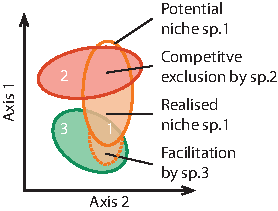
\includegraphics{./1_Introduction/graphics/niches.pdf}
  \caption[Different niches]{The potential niche of the \textcolor{myOrange}{focal} species is reduced by competition interaction with \textcolor{myRed}{species 2}, but extended by facilitation interaction with \textcolor{myGreen}{species 3}. This representation of the niche requires the knowledge of the effects of both abiotic factors and all pairwise interactions with other species. A more mechanistic approach of the niche should be considered in IMBs.}
  \label{fig:niche}
\end{marginfigure}

Similarly \textemph{facilitation} interactions also affect inderectly the levels of resources experienced by the focal plant, but in a way that is positive for the focal plant. So they widen realised niche outside the potential niche (see interaction between species 1 and 3 in figure \ref{fig:niche}). There are hypothesised to be larger along a stress gradient, where competition interactions are filtered out because they do not allow species maintenance and only positive interactions remain. Such relationships are dependent on the couple of species considered and may change depending on conditions \parencite{callaway_phenotypic_2003}.

\paragraph{Fundamental niche}
 From the point of view of the focal plant, these interactions only exist through the changes in resource availability (even if plants are able to identify their neighbours). In this sense, we can see potential and realised niches as displacements of the fundamental niche (niche defined in term experienced conditions, stresses and resources) within spaces defined by abiotic variables or biotic variables. From this framework, the fundamental niche, or conditions experienced by the focal plant, is the stronger representation of the species niche and the realised niche (abiotic and biotic filters on the niche) emerge from the effects of external factors on this experienced environment.

This point of view should be adopted in models \parencite{berger_competition_2008} because it allows the representation of both abiotic and biotic factors in a shared and generic framework. This is an improvement in comparison to model requiring matrix of interaction coefficient between species. Such matrix, in addition to be hard to parametrise, cannot be used in a framework of dynamic strategies. Modelling effort should instead be on explicit temporal and spatial dynamics of resource dynamics. Plant interactions would be captures by the effects of plant functioning (reduction of resource levels in relation to plant growth and resource use) on these dynamics \parencite{berger_competition_2008, morin_comparing_2009}.
%Biotic filtering - realised niche.

%Abiotic drivers main tnhing at global scale... Then interactions and competition.

\textbf{The concept of ecological niche serves as a great tool for theoretical research on coexistence. It encompasses in a convenient way both abiotic and biotic filters of one species distribution. While traditional view of the niche require to consider both abiotic filters and pairwise interaction, fundamental niches and resource dynamics modelling offer an alternative to model realised niche as an emergent property of the model.}


%-----------------------------------------------------------------------------------------
\subsection{The complexity of coexistence}

\paragraph{The question of coexistence}
If ones want to better understand and predict dynamics of complex systems, they first need to understand how such complex is assembled. Niches can be used to characterised a range of habitats a plant can live in, but because of complex inter-specific interactions, determining the final composition of a community from the list of species that can live in this habitat is not easy. If it is easy to observe diverse ecosystems (from bacteria, to plants, insects or algea), it is challenging to determine the processes that 1) group the entities together (in time and space), 2) maintain an apparent stability in the group composition (at least at a certain spatial and temporal scale). 
We can image imagine biotic filtering as an physical filter, the same way abiotic filter is often illustrated, but this image does not translate the dynamic and complex nature of underlying processes. Biotic filtering emerge as the result of all the interactions between the entities that make it through the other filters. And how these interactions, direct or indirect, play together determines the stability of the diversity.\\

To predict the outcome of competition interactions multiple theories have been developed. Among these theories, we can cite two that have different perspective on the same question: how do species whering resources coexist in an homogeneous environment?

\cite{chesson_mechanisms_2000} tends to have a population dynamic view of the system and identifies two types of processes that promote coexistence: (1) stabilizing mechanisms, (2) equalizing mechanisms. The former are required to stable coexistence as it a condition of invasibility. In other words, plants can coexist only if one species can invade the other. The condition to such invasion is that the species at low density growth better that the species at high density. This is the case if intra-specific competition is higher than inter-specific competition. Equalizing mechanisms are processes that diminish the fitness differences between the species, without ensuring stable coexitence. This framework is extended by \cite{adler_niche_2007} in the modern coexistence theory. It states that niche differences and fitness differences are the two mains axis of species coexistence. They make the assumption that niche differences define the relative strength of inter-specific versus intra-specific competition. The larger the differences between niches, the thiner is the overlap, and the weaker the inter-specific interactions. Therefore, this can be related to stabilizing mechanisms in \cite{chesson_general_2000}. On the other end, fitness differences also impact coexistence. The lower the differences, larger are the chances species coexist. The importance of niche differences required for stable coexistence decrease with the decrease in fitness differences.

In the other hand, Tilman elaborates a theory \cite{tilman_resource_1982, tilman_plant_1988} around resource use more in line with the idea of fundamental niche expressed in previous paragraph, the contemporary niche theory. Species are characterised by the impact they have on the resource, and they use the resource for growth. Competition is in favour of the species with the lowest requirement for the resource because competition leads to resource deprivation it can survive. But coexistence if there is more than one limiting resource. In this case, coexistence can be achieve if species have a stronger impact on the resource from which they benefit the most (and intersecting zero net growth isoclines). 


These two theories give strong conditions for stable coexistence, however they required simplifying hypotheses (all other things being equal, homogeneous environment) that are not met in natural environments. Despite their different appraoches, these theories can be united as demonstrated by  \cite{letten_linking_2017} if the impact and benefit coefficients from contemporary niche theory are transltaed into niche and fitness differences. Despite this unified theory, they applied to a too limited range of situation to be applicable in the context of diverse mountain grasslands.
%
%
%
%Focus on interaction: chesson modern coexistence theory.\\
%
%Chesson vs Tilman. 
%Chesson focuses on interaction and 2 by species, give central idea of stabilizing vs fitness difference.\\
%Tilman focuses more on resources, how the use and impact on resources affect competition and can enable conexistence, but limited coexistence according to this criterion: plankton paradox. No heterogeneity, no temporal dynamics\\
%
%Other things being equal hypothesis (in models at least) does not allow the full diversity to emerge.\


%Plankton paradox in homogeneous system, where abiotic and dispersion should have little role into maintenance of species diversity.\\


%\textbf{One mechanisms alone seems to not be enough to explain fantastic diversity observed in natural ecosystems. However there are multiple theoretical mechanisms that support species diversity and that should taken into account in community models: diversity of resources, spatial and temporal variability, frequency dependent effects, etc...}


\textbf{Plant community require strong coexistence mechanisms to maintain species richness. Single theories fail to predict high diversity observed in plant communities such as natural mountain grasslands. However, high dimension coexistence processes and complexity seems to be an answer to the biodiversity paradox. In addition to niche based coexistence processes, other mechanisms that promote coexistence must be considered.}




% _______________________________________________________________________________________
 \subsection{Variability and dynamics: driven by the resource}


%-----------------------------------------------------------------------------------------
%\subsection{The complexity of community dynamics} % not very informative title%

Resource dynamics, even with constant influx, seems to be the key of understanding plant interactions and dynamics according to Tilman \cite{tilman_plant_1988}. Can the resource distribution is time and space explain coexistence?

\paragraph{Community dynamics}

In Tilman's perspective, resources are driven by two things, external influx and internal (to the system) consumption or cycle. The system strucutre and composition is responsible for resource dynamics as much as external influx. And these dynamics alter the structure of the community and change the hierarchy within the community. This cycle is well illustrated by the cycles we can observe in forest systems and gaps models. Mature forests produce big trees that fall down and create perturbation within the system. The resulting hole in the canopy allows for pioneer species to invade this space without competition. While they grow, other slower species are in shadows and must tolerate this competition, and grow enough to out-compete first established species. Because there is trade-of between potential growth and shade tolerance allowing this cycle to set up, there is a succession dynamic after each perturbation of the systems. These local events of perturbation support coexistence as a large scale, coexistence that can be captured by spatially explicit models \cite{chave_study_1999, falster_plant:_2016}.

\paragraph{Temporal heterogeneity}

\begin{marginfigure}
    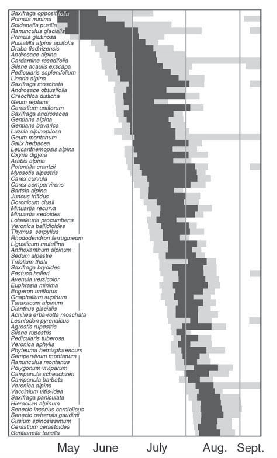
\includegraphics{./1_Introduction/graphics/flowering_m.pdf}
  \caption[Flowering periods of alpine species]{Diversity of flowering periods of alpine species. Evidence of succession in grassland ecosystems. From \cite{korner_alpine_2003}.}
  \label{fig:flowering}
\end{marginfigure}

Such drastic dynamics do not exist in mountain grasslands communities. But the natural temporal variability of resources due to contrasted seasons, also drives diversity in growth strategies. Coexistence comes the existence of multiple climatic contexts at the same place (but not the same time). As plants cannot be the most competitive species for any given condition in the whole range of conditions experienced in mountain habitats, there is a succession of species at the top of competition hierarchy \parencite{adler_climate_2006} (see figure \ref{fig:storage_effect} for illustration). The diversity of flowering periods in figure \ref{fig:flowering} is an evidence of this succession dynamics.

\begin{figure}%[tb]
    \classiccaptionstyle
\sidebysidecaption{0.60\textwidth}{0.3\textwidth}{%
    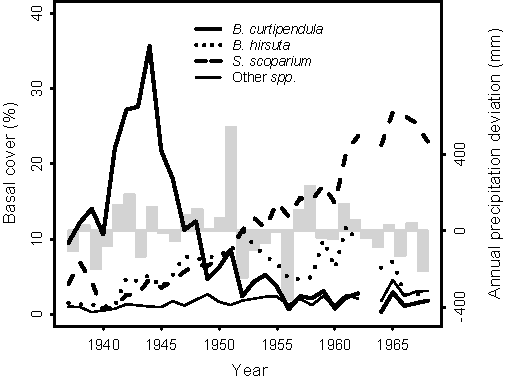
\includegraphics[width=1\linewidth]{./1_Introduction/graphics/succession.pdf}%
}{%
  \caption[Changes in dominance for 3 grassland species]{Changes in observed basal cover for 3 grassland species. This variation in hierarchy illustrate the succession in grassland communities and the storage effect due to the stabilizing effect of climatic variation promoting coexistence. See details in original study by \cite{adler_climate_2006}.}
  \label{fig:storage_effect}
  }
\end{figure}

This mechanism promoting coexistence because of succession dominance driven by temporal changes in environmental condition is called storage effect. The species grow when the conditions match their niche, and store the gains to wait until next favourable conditions. This term is generally applied to yearly variations, but the idea can be applied for variations within a growing season, allowing growth and storage until next season.

%
%from tilman: dynamics of resources
%
%gap model, succession in forest
%
%less structure in grasslands, but also diversity between early and late 
%
%
%
% Succession coexistence and forest models. Dynamics of resources, influx versus impact. Storage effects. Heterogeneity. But how does it link to traits.

%\textbf{From the multiple first attends to explain coexistence with one particular mechanism, scientific community realised that indeed multiple mechanisms are at work to make species diversity in ecological community. 
%multiple drivers that filter down. + temporal effect (metacommunity, invasion, equilibrium vs long transitions)
 % This multiplicity highlight the need for unifying framework able to cover this diversity of mechanisms and dimensions.}
 
 
\paragraph{Spatial heterogeneity}

The temporal variations have a stabilizing effect on coexistence \cite{tilman_plant_1984}, but maybe more intuitively, spatial heterogeneity also promotes coexistence. Indeed, spatial variations of conditions at small scale create multiple niches that allows for diversity if measured at higher scale. This spatial heterogeneity can be overlooked, but in the context of mountain grasslands where plants are generally small due to high stress levels and very fine scale heterogeneity due to terrain texture it can play as a strong stabilizing mechanism.

%
%tilman 1982, spatial
%chesson, 1994, temp, 
%storage effect admer 2006
%even if stochasticity can reduce coexistence. Fine scale heterogeneity is rarely taken into account, but can play an important role, especially with small individuals.

\textbf{Spatial and temporal heterogeneity play a major role in coexistence maintenance by creating various opportunity, or niches, in a given ecosystem. Internal dynamic variation of conditions also support stable coexistence.}

\subsection{The complexity of diversity}

\paragraph{Larger scales dynamics}

While resource use strategies and resource heterogeneity are important mechanisms for diversity, dispersal processes and meta-community dynamics should also be considered.

Role of meta community and dispersion dynamcis, network effects

\paragraph{Embrace complexity}

\parencite{clark_resolving_2007}: coexistence is highly dimensional


 
 % conclusion of the section/chapter:
 \textbf{The evaluation of services relies on a good representation of the plant community and its essential properties. To represent complex interacting systems like vegetation communities, descriptive approaches are not sufficient and driving processes must be considered. Explicit heterogeneity and dynamics of the resources is key to understand and model filtering processes, coexistence mechanisms and community dynamics. Modelling both community properties and resource dynamics require understanding of plant functioning and diverse growth strategies.}
 
 
% #######################################################################################
%\chapter{Considering strategies and functional traits}

\chapter{How to represent plant community}

All plants share the same pool of essential resources and similar physiological processes of assimilation and allocation, however species differ by their growth rates and niches. How such difference emerge  from common functioning framework? Species differ on parameters that characterise this functioning. The challenge of modern community ecology is to determine the trajectories existing ecosystem will follow under new environmental conditions. Species centred approaches, because they are limited to the knowledge of existing response patterns to existing gradients, cannot tackle this 
problem. How can changes of the representation of plant allow generalisation of plant functioning to new conditions?
%Same resources: even more difficult to understand coexistence. Must have differences on how they gather and use these resources. Species is not a handy tool to describe differences in functioning and strategies. Shift in paradigm needed.

% _______________________________________________________________________________________
\section{The continuity of functional ecology}

\subsection{Shift in paradigm: traits and patterns}
 blabla bla 

Measure of respiration, assimilation : better insight on the differences between species. Better understanding of plant functioning. Also show that there is a continum in plant functioning. This continuum is in line with the observed continum of community.

\paragraph{A shift needed}

Classical use of niche theory can be observed in Species Distribution Models (SDMs) that link the probability of presence of one species to multidimensional description of an habitat. The environmental variables are literally used as the dimensions of the Hutchinsonian niche, and directly link the species to its fitness in a given environment (see figure \ref{fig:paradigm_shift}, first row). This method is widely used to model environmental niche, but some can also include species interactions to incorporate explicitly biotic filter. SMDs have good theoretical support and have a lot of practical applications, however their strength is reduced at the scale of the community where the biotic filtering processes and fine scales dynamics take the advantage over large scale abiotic filtering. Also, because they require a lot of data for any given species, they lack generalisation properties to be applied to rich communities. Community dynamics require fine scale plant functioning processes to capture the effects of small scales variability and plant interactions, drivers of coexistence. 

This example of modelling approach based on a species centred framework reveals the weaknesses of this framework. The distribution of a species along gradients, or its niche, while it can be capture by abiotic variables, is primarly determined by the fitness components (and wheather or not they lead to a positive fitness): growth, survival, reproduction. These variables are not intrinsic properties of species, but emerge from the interaction between physiological processes (carbon assimilation by photsynthesis, water absorption, organic matter allocation, etc...) and the environmental conditions. Only considering these processes allow to explicit and decompose plant functioning, and therefore model it in new combinations of environmental conditions.

\begin{figure}
    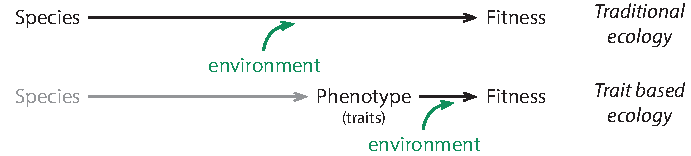
\includegraphics[width=1\linewidth]{./2_PP/Figures/Concepts/species_to_fitness.pdf}
  \caption[From discrete to continuous link between species and fitness]{The shift toward trait based ecology allows for the decomposition of the link between species and fitness determined by the environment. On one hand, the link between species and traits is better characterised by standardised protocols and the use of databases such as TRY \parencite{TRY}. On the other hand, the link between phenotypes (defined by trait values) and fitness can be generalised and the role of environment on this relationship better understood.}
  \label{fig:paradigm_shift}
\end{figure}

Most of plant species share the same growth, survival and reproduction processes, but they still differ in these aspect as a function of the abiotic and biotic environment. The solution to shift from species centred paradigm, and its couple habitats-species (or species-environment-abundance like in SDMs), is to explicit the phenotype of these species. By using functional traits to define the phenotype of a species, ecologist can limit the representation effort to the link between traits and fitness physiological properties \parencite{reich_leaf_1992}, and then link species to traits with simpler data collection procedure \parencite{cornelissen_handbook_2003} (see figure \ref{fig:paradigm_shift}, second row).


This shift in paradigm allows for a simpler and functional representation of plant species, that can be latter link to physiological or ecological processes.

%diaz, lavorel, glopnet and try

%this shift worked: falster, 


\paragraph{The rise of functional traits}

The functional traits allows to decompose the link between species and fitness, but requires an extra step as two links must be defined. 

Collection of multiple trait sampling.

\paragraph{Traits and gradients}


change of traits along gradients. Is it interesting?



\textbf{The complexity of coexistence and community dynamics processes could not be captured with traditional species centred ecology. The last two decades saw the rise of functional ecology and its ability to capture quantitatively relationship between vegetation and abiotic gradients. The capacity to }

\subsection{Understanding interaction and competition: a question of symmetry?}

Functional traits can be used to determine the response of species or communities to an abiotic factors, or link morphological traits to physiology. It is also argued that they can capture responses to biotic factors. Traits could be used to 

CAUTION: do not mistake symmetry of competition (function of delta tratis) with form of competition (georges presentation). 


niches and gradient - symetric vs hierarchical 

symetric an assymetric interaction: it could change the interpretation: identify which traits are in what case.


\parencite{kraft_functional_2008}
often need to use multiple traits \parencite{kraft_plant_2015}


traits used as a proxy for plant interaction and competition. /!\ can be context dependent \parencite{gallaway_2003}.

but non transitivity: key role in maintenance diversity \cite{levine_beyond_2017}.

\textbf{Traits are good proxy for competitive interaction and fitness differences. .. a bit more complex. If the interaction is transitive, a strong asymmetric pattern can be observed between interaction effects and trait differences, while symmetric interaction reveal niche differentiation processes. Despite these observed relationship, alternative mechanistic solutions must be adopted to capture the multi-dimensional and context-dependent nature of plant interactions.}


\textbf{The paradigm shift toward functional ecology allowed the shift from discrete to continuous representation of species. This change makes easier the representation and study of plant communities, especially along conditions or management gradient. Traits are also used to study plant interactions.  Trait approaches offer a functional link between morphology and physiology that has great potential in generalising environmental effect on phenotype-fitness relationship. However, the need for multiple traits to capture plant niche differences or similar response patterns of multiple traits suggest underlying structure within trait assemblage. Understanding this structure and how it relates to community dynamics external drivers is crucial in the representation of diverse communities. } 

%Despite the advantages of functional traits, close comparisons and links with theoretical approaches should be used carefully, and underlying assumptions should be interrogated.




% _______________________________________________________________________________________
\section{How trade-offs make strategy space}

%-----------------------------------------------------------------------------------------
\subsection{Trade-offs: capture constraints on species differences}

\paragraph{Leaf Economic Spectrum}
The functional link that is observed between some morphological traits and physiological traits suggests underlying processes that link these traits together. It appears that multiple traits are correlated together at the global scale between species \parencite{reich_evolution_2003,	 wright_worldwide_2004, chave_towards_2009, reich_world-wide_2014} and within species \parencite{hu_novel_2015}. This coorelation between functional traits of the leaf was described at a global scale by \cite{wright_worldwide_2004}. The \textemph{Leaf Economic Spectrum} (LES), defined by these correlations between multiple traits, draws a continuum of strategies. It spreads from species with high resource acquisition rates and rapid growth rates but low tissue lifespan, to species with longer tissue lifespan but lower growth rates. This is a clear description of a \textemph{trade-off} between strategies, opposing exploitative strategies (high Specific Leaf Area (SLA), high Leaf Nitrogen Content (LNC) and low Leaf LifeSpan (LLS)) to conservative strategies.


\begin{marginfigure}
    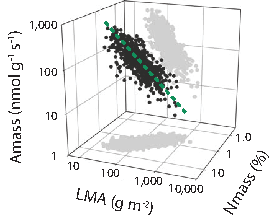
\includegraphics{./Figures/LES1_m.pdf}
  \caption[Leaf Economic Spectrum]{Three dimensions of the LES. Correlation of Leaf Mass Area, assimilation rate per mass unit and nitrogen concentration. This correlation reduces three dimensions (more dimensions not shown) into one axis (\textcolor{myGreen}{- -}).}
  \label{fg:insurance}
\end{marginfigure}

This axis of differentiation allows ecologist to link quantitative measures to types of strategies that better capture diversity of strategies than discrete typology. These strategies are translated in traits, traits that can be translated into physiological processes parameters, then into components of fitness.

In addition to a quantitative measure of species strategies, such trade-offs simplify a lot trait-based approaches. While many variables can be measured on one individual, correlations between these variables reduce the number of dimensions to considered. This simplification cannot be better illustrated by the work of \cite{diaz_plant_2004} that demonstrate the existence of two major axis of "evolutionary specialisation" that explain most (41\%) of trait variability: siez related traits, and resource use speed traits. Similar evidence is also found at global scale in addition to evidence for high levels of coordination between axis \parencite{diaz_global_2016}.


Similar correlations could be found in roots \cite{ ryser_importance_1996, reich_world-wide_2014}

Where does it come from : shipley : morhpological constraints (as for seed size and seedling growth and survival), hard frontier plus soft frontier (small figure).

Diversity of mech: diveristy of strategies. more or less independent.\\

\textbf{Trait-based ecology rapidly lead to the observation of trait correlations and trait syndromes between plants. These axes of differentiation emerge from processes that constraint plant strategies. Better characterisation of these constraint should allow a better representation of plant functional diversity.}

%-----------------------------------------------------------------------------------------
\subsection{Strategy-spaces made of trade-offs}

Global functional trait dataset and databases revealed global scale correlations between traits. These correlations, or trade-offs, simplify the representation of plant species \parencite{diaz_global_2016} and translate fundamental axis of strategy differentiation \parencite{reich_world-wilde_2013}. Yet, plant community exhibit extraordinary species and functional diversity suggesting that not all traits are correlated. Trade-offs emerge because of hard (physical, chemical or biological) and soft (competitive pressure) constraints on combinations of functional traits. Therefore, for a given couple of traits, the physical independence of traits and the independence of ecological processes they are involved in should insure the absence of trade-offs between those. While some traits are related to multiple physiological processes (a composite traits like SLA is involved in water regulation, but also light capture), traits are often specific to a processes...
Same number of strategy axis than filtering processes. (avoidance vs resistance, drougth, frost, but could be applied to competition for resources )


reich, wright, shipley, diaz.

\paragraph{Empirical evidence}

support of CSR triangle \cite{frenette-dussault_functional_2012, pierce_allocating_2013}

\textbf{The multiplicity of processes shaping vegetation systems leads to similar constrained diversity in plant strategies. These strategies are captured in a strategy space drawn by independent trade-offs tightly related to functional traits. These functional trade-offs have great potential in the representation of a functioning plant diversity, while parameter set allows easy characeterisation of species and communities.}



% _______________________________________________________________________________________
\section{How traits link to ecosystem properties}

The link between community properties and ecosystem services has been mentioned in chapter \ref{part:introduction}, this section develops processes involved and how functional traits are integrated into this link.

%-----------------------------------------------------------------------------------------
\subsection{Mass Ratio Hypothesis, Community Weighted Means, and functional identity}

As explained, plant species, based on their identity, provide ecosystem services. Some of these services are direct consequences of the characteristic of the species and their functioning. The greater the abundance of a species that supply particular ...

Because functional traits are quantitative variables, they can be manipulated more easily than factors. Therefore, while phytosociology describe vegetation communities with broad types and approximate abundances, trait-based ecology benefit from this continuity to characterise mean properties of community. The \textemph{Community Weighted Mean} of a functional trait is the average of species specific trait values weighted by the relative abundance of each species, and correspond to a mathematical application of the mass ratio hypothesis. These summary variables define the communities in a quantitative way similar as functional trait for species. In addition to be quantitative, it is functional and responses to disturbing factors can be predicted \parencite{lavorel_predicting_2002}.


grime1998, shipley 2006
\textbf{According to the Mass Ratio Hypothesis, some properties of the community directly scale to the characteristics of the most abundant species. In this hypothesis, the \textemph{functional identity}, defined by functional trait values, has more importance than the identity of the species. Community Weighted Mean measures generalise this hypothesis using mean species trait values. While these tools can link community composition to ecosystem properties and services, they require precise measures of plant functional traits to be reliable.}

%-----------------------------------------------------------------------------------------
\subsection{Benefits of diversity}

Certain processes are determined by the most abundant species of a community, but other services and functions may result from the properties of the group. Diversity is the most important property of an ecosystem or a community for wide audience. This measure is peculiar to groups of organisms and plays a major role in its functioning and the services it provides. Diversity can refer to species richness or functional diversity. The former quantifies the number of species present in a habitat and can take into account the relative abundance of the species. Many indexes can be used to measure this variable representing different perspective or aspect of the metrics (see \cite{chalmandrier_communities_2015} for exhaustive information).

Empirical studies demonstrate the importance of diversity for multi-dimensional services ... Services are: ......

Diversity also supports functions and other properties of the system. Multiple mechanisms explain this multiplicity contained in the measure of diversity. 


\begin{marginfigure}
    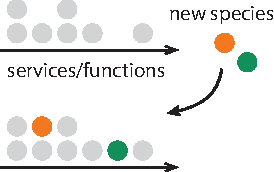
\includegraphics{./Figures/insurance_m.pdf}
  \caption[Diversity insurance effect]{Insurance and selection effects. New species increasing diversity either reinforce existing function (\textcolor{myOrange}{$\bullet$}), or provide new function (\textcolor{myGreen}{$\bullet$})}
  \label{fig:insurance}
\end{marginfigure}


First importance of species richness in found in the insurance effect that prevent the loss of a function or a service with the loss of a species by insuring that multiple species provide such function or service. Another way of seeing this notion is the selection effect that states that increasing diversity increases the potential number of services provided by the community, as each species added can provide new function/service (or at worst reinforce already present ones). This second concept is at the edge of the insurance effect

benefit of species diversity: insurance effect - portfolio effect ?

selection, niche complementarity

what about functional convergence

productivity 

\textbf{}

\subsection{Productivity: both community property and ecosystem services}

Productivity of a plant community is mostly sensitive to abiotic conditions (precipitation and temperature). 
Productivity as a marker of abiotic conditions and 

Productivity as a property: depends on the community structure and properties. Leads different services.

Productivity as a service itself: production (fodder in this case, but OM in forests).

\textbf{}

%-----------------------------------------------------------------------------------------
\subsection{Trade-offs in ecosystem properties}

lavorel 2012 : trade-off  \parencite{lavorel_how_2012}
traits - related to trade-off in ES bundles, mostly driven by climate change (rather than management) \parencite{lamarque_plant_2014} limits ?
%\textbf{}


% Section/chapter conclusion
\textbf{The shift from species centred paradigm to trait approaches unlocked numerous discoveries in plant community ecology. In addition to facilitate the study of the effect of abiotic conditions and biotic interaction, traits can be used to describe the community and its main properties to evaluate ecosystem services.}

%\textbf{However, the accumulation of trait measurements useful for the study of gradient response patterns and community structure, also reveals the variable nature of traits.}



% _______________________________________________________________________________________
\section{Modelling diverse plant community}

Modelling mainly consist in deciding what is important considering and worth representing. The choice of how an entity or a mechanisms is represented also correspond this decision making. While considering vegetation community the choice can be on the resources needed, the type of perturbation, or the part of the life cycle of most importance. For vegetation models for the study of community properties and dynamics, the representation of the interactions of multiple species is key. Strategy space concepts offers a great solution to both the interactions and the diversity of species, while also informing the modellers of the communities' properties.

%-----------------------------------------------------------------------------------------
\subsection{How strategy space open vegetation modelling}

%In a mechanistic model with multiple species, strategy space are simplified ways to define multiple species. Species identity is fully defined by its position in this space of species specific parameters.

\paragraph{Theory to traits}

Plant diversity is expressed and in visible to anyone by the variation in shapes and colors, scents and growth forms, but this diversity is the demonstration of the multiplicity of strategies. In a early attempt to make sense of this diversity of strategy \cite{grime_evidence_1977} theorise the existence of two type of constraints that shape plant communities: perturbations and stress. The perturbation axis captures the variability of community drivers, while the stress axis captures how conditions facilitate or make difficult plant establishment. They draw a two-dimensional space where three regions can be invaded\sidenote{high stress and high perturbation regions does not allow establishment}, corresponding to three different strategies: competitive (C) in low stress-low perturbations region, stress tolerant (S) in high stress-low perturbations region, ruderal (R) in low stress-high perturbations region, forming Grime's triangle (\see figure \ref{fig:grime_triangle}).

\begin{marginfigure}
    \includegraphics{./Figures/Grime_triangle.pdf}
  \caption[Diversity insurance effect]{Grime's triangle. Competitive (C), stress tolerant (S), and ruderale (R) strategies are dominant in the three regions of the perturbations-stress space.}
  \label{fig:grime_triangle}
\end{marginfigure}

Grime's triangle set the basis for strategy space, and the broad meaning of \textit{stress} and \textit{perturbations} terms allow them to be applied to various conditions. However, the diversity of types of stresses (drought, cold, nutrient availability) and perturbations (predation, fire, avalanches etc...) cannot be specificaly captured by such wide concepts. \cite{westoby_leaf-height-seed_1998} highlight the difficulty to use such space and its incapacity to explain some patterns. According to him, a strategy space\sidenote{called Plant Ecology Strategy Scheme (PESS) in his paper} should: 
\begin{itemize}
\item "express meaningful differences in ecological behaviour between species";
\item allows to "position a plant species from anywhere in the world within";
\item be composed of attributes that "require little enough effort to estimate";
\item lets "possible to quantify the extent to which the [strategy-space] captures variation in other plant attributes".
\end{itemize}
He proposes to use functional traits to meet these criteria of functional differences, generalisation, and practicality. Three traits capture the components of Grime's triangle:
\begin{itemize}
\item Specific Leaf Area (denoted L): captures the speed of return of investment of carbon in leaf, as latter highlighted in the LES. High SLA is generally associated to competitive species that capture a lot of light and have a high growth rate. At the other end of the spectrum, low SLA species are more stress tolerant. This axis is the practical equivalent to hte axis CS in GRime's triangle.
\item Height at maturity(H): race to the light (but not time fixed as protocol for functional trait encouraged it), but also capture ruderal axis (time interval between perturbations)
\item Seed mass (S): expresses the capacity of a species to invade freshly disturbed environments or the competitive advantage seedlings possess with a larger starting carbon pool. This trade-off between competitive strength of seedlings against chance of invading freshly disturbed environment capture well the CR axis of Grime's triangle.
\end{itemize}
The LHS strategy space proposed by Westoby has the advantage 


\paragraph{In DGVMs}

Strategy space proposed by Westoby 

Dynamics Global Vegetation Models tend to use such strategy spaces to model high diversity with limited number of traits. 

Simplification: limited number of straits: DVGMs

translate traits into physiology: easy

diversity of strategies

specific trade-off related to the context \parencite{scheiter_impacts_2009}

\paragraph{In IBMs}

why not too much on IBMs (but Reineking, Marechaud ?, falster, meh, I guess that Lohier's and Maire's are sort of strategy space) - because lower community models at this scale: gap to fill.

But when it's used: break the growth function that links phenotype, genotype and environment ( see figure \ref{fig:paradigm_shift}). Same growth function: no need for specific parameters: smae rules for all, but different phenotypes. (the concept of genotype and phenoptype would merge for functional traits, if there was not other control on other aspects, phenotype defines itself). This is important as it allows for intra-specific variations that would necessite more complex function in the first paradigm. 

The growth function, in a simulation model includes all steps from resource gathering and transformation, biomass allocation and phenotype alteration (\textit{e.g.} frost, graing \textit{etc}...), takes as inputs the phenotype and environment, and gives the new state of the phenotype (and environment). 

 figure \ref{fig:paradigm_shift}

This last paragraph is important to link with the plasticity in a later paragraph.


%-----------------------------------------------------------------------------------------
\subsection{How models inform us on properties and dynamics}

\textbf{The use of strategy spaces in models allows the representation of high diversity in a common plant functioning framework requiring limited number of parameters. Such approaches are very useful to follow the dynamics of communities in a mechanistic framework. Individual models tends to ignore such simplifications procedure and relies on direct measure of traits of interest because they generally integrate a limited number of species. IBMS can take advantage of trade-offs and simple strategy spaces to model diverse communities at small scales while keeping biological mechanisms at their core. However, model based of strategy space tend to consider mean individuals and ignore the individual variations.}


% #######################################################################################
\chapter{The importance of phenotypic plasticity as a specific case intra-specific variability}

% _______________________________________________________________________________________
\section{Intra-specific variability change the rules}


%-----------------------------------------------------------------------------------------
\subsection{Increasing interest in intra-specific variations}

Trait approaches emergences lead to a better understanding of general patterns of community responses to drivers and of trade-offs in plant functioning. But with the accumulation of large trait databases the importance of \textemph{intra-specific variability} could not be ignored.

\paragraph{Extend}

The extend of the intra-specific variation is a big question as some ecologists point out because trait based approaches make sense only if inter-specific differences are greater than intra-specific differences. While this can be discussed, high functional variability within the species would weaken theories and generalisation based of mean traits. \cite{violle_return_2012} suggest that the extend of within population variability relatively to within community variability should be considered and avoid mistakes in the estimation of coexistence mechanisms. Ignoring intra-specific variability lead to underestimation of niche overlapping, plastic response to neighbours or the fraction of resource a species can used. Multiple studies focused on the extend of functional intra-specific variability \parencite{albert_intraspecific_2010, albert_multi-trait_2010} and how to disentangle this vairability from species turn-over \parencite{leps_community_2011} in community response. These studies show contrasting results between traits and levels. \cite{albert_multi-trait_2010} demonstrate a within species variability explaining between 20\% and 40\% of total trait variance, and \cite{siefert_global_2015} note similar levels, but this fraction tends to decrease with the increasing community diversity. They also show that the strategic differentiation between exploitative and conservative species is robust to these variations. It appears that all traits are not variable to the same degree and traits like SLA, height, LNC and LDMC are relatively variable while leaf morphology traits variability is lower\cite{siefert_global_2015}. 

The variability of multiple traits certainly impacts the functional diversity \parencite{de_bello_quantifying_2011, albert_importance_2012}. All indexes are not sensitive to the same degree, with single trait measure being the most sensitive, but should be used carefully to draw interpretation of ecological pattern linked to functional diversity. To overcome this difficulty and disentangle the effects of the different forms of functional diversity specific indexes are developed \parencite{de_bello_quantifying_2011}.

The relative extend of intra-specific variability depends on the trait, spatial extend and species richness, but not on climatic conditions \parencite{siefert_global_2015} suggesting general mechanisms 
%
%\parencite{violle_return_2012}
%ISV is relatively large, ignored in numerous studies, butshould not. Viole argue that may alter our capacity to estimate and understand capacity of species to coexist \cite{jung_intraspecific_2010} suggest to use hierarchical measure of variance to define the source of variation and that would allow to better explain coexistence mechanisms (niche vs individual variation vs neutral theories)
%
%
%\parencite{siefert_global_2015}
%but intra-specific variation change between traits. Most variable traits being: ...

%\cite{leps_community_2011}

%More interest in trait distribution, variability and diversity. $\rightarrow$ Get to look at intra-specific variability.\\
%\cite{albert_intraspecific_2010}


%\paragraph{}

The fact that some traits are variable while others are not implies that some mechanisms structure this variability.
%Intra-specific variability can affect species in multiple ways that are discussed later, 
A way to identify such effects is to look if variability is structured along environmental gradients, suggesting adaptation mechanisms.

Along such gradients trait variability for traits like SLA \parencite{poorter_causes_2009} of leaf mass fraction (LMF) \parencite{poorter_biomass_2012} follows similar patterns as inter-specidic response \parencite{niinemets_global-scale_2001}, with increasing SLA along precipitation and temperature gradient, and decreasing SLA along radiance gradient (leaf mass fraction shows similar responses). These responses suggest strong constraints (similar to the ones that shape inter-specific differences) shaping this variability. However, species may vary in their response \parencite{kichenin_contrasting_2013}. This contrast can be explained by differences in position around a bell-shape response curve around the optimum (see \cite{albert_intraspecific_2010} for more details). \cite{kichenin_contrasting_2013} argue that it is not the case because along a wide gradient not bell shape response curve is observed for any trait or species.

This additional level of variability is not always in the same direction as community response driven by turn-over \parencite{albert_intraspecific_2010, kichenin_contrasting_2013, jung_intraspecific_2014} leading to difficulties to predict the response of the community. These levels must be disentangled, in order to do that, mechanisms underlying intra-specific variability must be understood. This is particularly important because they have multiple effects on how we model community dynamics and understand coexistence mechanisms \cite{bolnick_why_2011, violle_return_2012}.
%
%but if mechanisms are well identified, response patterns not so much.
%
%\parencite{poorter_biomass_2012}
%\parencite{poorter_causes_2009} strong response to light (-), water (+) and temperature decrease (-)
%- suggests selection or plasticity.
%
%\parencite{kichenin_contrasting_2013}
%Jung: not always in the same way \parencite{jung_intraspecific_2014}\\
%\parencite{wellstein_intraspecific_2013} local adaptation, clonal traits
%

\textbf{After the emergence of trait-based ecology and its high potential, recent focus on intra-specific trait variability question the strength of such approaches. While  intra-specific variability  does not negate numerous conclusions from previous work, because of its large extend and how it alters functional diversity, its effects on community dynamic processes must be interrogated, and underlying mechanisms investigated.}

%-----------------------------------------------------------------------------------------
\subsection{Contrasting effects of intra-specific variations}

Intra-specific variability impacts coexistence mechanisms and community properties in multiple ways, the following paragraphs are not an exhaustive list of all ways ISV affect community properties or our understanding of coexistence mechanisms, but a few contrasting examples to emphasis the need for better identification and understanding of underlying mechanisms. 

\paragraph{Jensen inequality}

Jensen inequality ... 
Intra-specific variability can affect 

Hart: why it is not enough

\paragraph{Niche}

ISV also 
effect of abiotic filtering

affect on realised niche

neighbours: avoid or increase competition


\paragraph{Contrasting effects}

specifically on diversity

callaway 2003 from competition to facilitation.

\cite{bolnick_why_2011}
\parencite{hart_how_2016}
\parencite{courbaud_intra-specific_2010}
\parencite{turcotte_phenotypic_2016}
\parencite{roscher_contrasting_2015}
\parencite{valladares_species_2015}
\parencite{barabas_effect_2016}
\parencite{jung_intraspecific_2010}

\textbf{The intra-specific variability has been observed to be an important part of community functional diversity, but also a way the community respond to changes in conditions. In addition to the empirical evidence of this importance, theoretical approaches support contrasting effects of such variations on coexistence mechanisms, evolutionary processes and community responses to climate event or invasion. It is crucial to disentangle different sources of intra-specific variability in order to their understand potential effect on ecosystem dynamics.}

%-----------------------------------------------------------------------------------------
\subsection{Beyond the mean and the bell-shape: towards more mechanisms in representing intra-specific variability}\label{subsection:bell-shape}

\paragraph{...}
There is a difference between how we obsere ISV, and why it emerges. What is random? Therefore it is  ... not good ... to apply such simplification of random effect onto theoretical models to predict the effect of intraspecific variability with strong assumption (observed on functional trait in wide spatial range, applied to interactions in homogeneous context) on how they translate onto interactions (done in Halt, check Boltnick) 
\cite{albert_intraspecific_2010} bell shape intra-specific response pattern along gradient, but doesn't stand according to \cite{kichenin_contrasting_2013}. Depends on trait and gradient... cannot assume that, need real quantification. ok if not a gradient response (or gradient is not known).
Bell shape can emerge from non measure gradient with linear response. 

Dewitt and Barabas.

The same way the neutral theory is simplifying and brings little understanding to underlying processes and relies on strong hypothesis, considering intra-specificity as a purely random mechanism is insufficient.\\
Bell shape do not appear in altitude gradient... inconsistencies between theory and empirical data\\
Strong theoretical hypothesis\\
refer to asymmetric and symmetric competition\\

\paragraph{...}
If most of changes are plasticity or selection: it changes the effects on interactions and niche.\\
What are the possible effects? probably it does not affect interaction like \parencite{hart_how_2016} supposes (even if they talk about variations, their conclusions may not be extendable to plastic variations). May change a lot the balance between abiotic filtering and biotic filtering. 

-- go to indivdual mechanisms, evolution could tackle genetic variations, physiology and ecology on ontogeny, and evolution and ecology on phenotypic plasticity


\textbf{Simple approaches to intra-specific variation constitute an improvement over mean approaches as they highlight processes ignored until now. However such approaches overlook the structure of the variability and underlying processes, leading to simplistic representations and potentially misinterpret the role and effect of this variability.}

% section/chapter conclusion

\textbf{%As ecology shifted from species to traits syndromes, it seems that it needs to go from syndromes to distributions and drivers.
Ecology shifted from species to traits syndromes with great success, but the intra-specific variability constitutes a great challenge for generalisation of observed patterns. By overlooking the processes that structure intra-specific variations, we might loose capacity to properly interpret the role of variability and refine our understanding of community functioning. The complexity of living communities requires to go further down and consider the individual scale. This is made possible by the accumulation of more and more numerous and detailed data, the improvement of statistical and new simulation tools. The question of the sources and drivers of intra-specific functional variability seems crucial to rise to the challenge it issues.}



% _______________________________________________________________________________________
\section{Phenotypic plasticity: a specific case of intra-specific variability}

Until now, the processes at the origin of intra-specific variability has not been discussed, but to understand how it can alter community properties it is necessary to differentiate the different sources of intra-specific variations as they work in different ways.

%-----------------------------------------------------------------------------------------
\subsection{The different sources of intra-specific variability}

Intra-specific variation can be caused by to two mechanisms: genetic variation and phenotypic plasticity. Genetic variation occurs when individuals from the same species have different genotypes, leading to different phneotype. On the other hand, phenotypic plasticity implies that a same genotype can lead to different phenotypes. Plasticity can involve epigenetic mechanisms \parencite{
zhang_epigenetic_2013, nicotra_adaptive_2015, beaman_evolution_2016} that blur the frontier between the two forms of intra-specific variability as epigenetic is a inheritable form of plasticity. It is transmitted to descendants but unlike genetic mutation is reversible. To keep thing simple, epigenetic phenomenons will not be discussed here.

Genetic variability (as well as epigenetic) can be detected in case of origin specific response, while if the variability is explain by the treatment, it is a plastic response \parencite{frei_plastic_2014}, and a large fraction of the variability observed in grasslands species is plastic response rather than genetic variation alone \parencite{frei_plastic_2014, merila_climate_2014}.

\cite{nicotra_plant_2010} provide a good review of plasticity mechanisms and the importance for adaptation to climate change. They advocate plasticity in functional traits should be considered in mechanistic models as they may play a central role in the speed and adaptiveness of community response to climate change.
%Nicotra : pl as a important mechanismfor plant to answer to climate change, shoud look at it.


\textbf{Intra-specific variability can be decomposed in two main types: genetic variability that seems to be closer to random processes envisioned in simple models of intra-specific variability, and phenotypic plasticity that specifically links variations of phenotype to differences in external conditions. These mechanisms of variations are under the control of both evolutionary and molecular processes, that need to be better understood to be disentangled and to better predict their effects on community dynamics.}

%-----------------------------------------------------------------------------------------
\subsection{What is phenotypic plasticity?}

Plasticity is a source of intra-specific variability, but biological processes leading to changes in phenotype can be complex. These paragraphs try to disentangle the different forms of plasticity and the underlying mechanisms.

\begin{fullwidth}
\begin{tcolorbox}[title=Molecular basis of phenotypic plasticity] %Toutes les options définies dans le préambule peuvent être définies aussi ici. J’ai juste gardé la possibilité de changer le titre de la box dans ma thèse
Phenotypic plasticity lies both in the perception of external conditions through sensor organ and signaling pathways (auxin pathway, root stones for gravity ...), and the integration of this information to alter the development plan. This integration must be coordinated at the scale of the plant according to rules or objectives, question partly explore in this work, but ultimately is applied at the cell levels.\\
\indent Because of the complexity and our partial understanding of these mechanisms, we will not attempt to model them. However I hope that this little overview of molecular mechanisms at the scale of the cell will give the reader an idea of the processes behind the abstract concepts used in this manuscript.\\

%\begin{figure}
    \includegraphics[width=1\linewidth]{./1_Introduction/graphics/molecular_basis.pdf}
  
%   \captionof{figure}{Caption}
   %\caption[Decomposition of plastic response]{Decomposition of phenotypic plasticity as a step between the genotype and the fitness. Phenotypic plasticity is the effect of environment on the link between genotype and phenotype. Plasticity can itself be decomposed in active plastic response that change the internal status of the individual (under genetic control) and passive response that result from inevitable effect of environment of the traits on the individual.}
%  \label{fig:plasticity_form}
%\end{figure}

The diversity of mechanisms and scales (both spatial and temporal) these processes can act inside of plant gives an idea of the diversity of strategies a plant can deploy to face changes of its environment. Considering this complexity, only a small fraction can be explored in such model as \model, but hopefully it will help make progress in our understanding of the role of these molecular mechanisms at the scale of the community.
\end{tcolorbox}
\end{fullwidth}






\paragraph{Forms of plasticity}
Phenotypic plasticity is the capacity of a species to produce individuals with the same genotype but different phenotypes. This difference in phenotype should be an active process, not the results of direct alteration of the phenotype by external factors without changes in internal functioning. This change in internal functioning process has the objective \sidenote{in the sense it has been selected because it provides this capacity} to match the phenotype with expected future conditions to maximise the individual fitness. The expression "expected future conditions" is key here, as it is this projection that drives the plasticity.
%Confusion, phenotypic plasticity is particular phenomenon, driven ...\\

\textit{Active plasticity is used for predominantly anticipatory, and often highly integrated, phenotypic changes in response to some environmental cue or signal, and reflect modifications of developmental pathways and regulatory genes.} Forsman - 2014\\


Passive plasticity, on the other hand, may stem from direct environmental influences on chemical, physiological and developmental processes, and is generally not considered anticipatory, but a mere consequence of the environment, such as stunted growth owing to low resource levels.\\


\begin{figure}
    \includegraphics[width=1\linewidth]{./2_PP/Figures/Concepts/genotype_to_phenotype.pdf}
  \caption[Decomposition of plastic response]{Decomposition of phenotypic plasticity as a step between the genotype and the fitness. Phenotypic plasticity is the effect of environment on the link between genotype and phenotype. Plasticity can itself be decomposed in active plastic response that change the internal status of the individual (under genetic control) and passive response that result from inevitable effect of environment of the traits on the individual.}
  \label{fig:plasticity_form}
\end{figure}

%\paragraph{Biological process}
% The details of the molecular changes that occur in a plastic response ). 
Active and passive plastic response can be discriminated by the position of the control: internal for active plasticity, or external for passive response. In the case of active plastic response, the signal from environment must be integrated (from physical or chemical to information) then transferred to response organs. These organs respond to the integrated signal by changes in their expression levels (\textit{internal status} in figure \ref{fig:plasticity_form}) as summarised in figure \ref{fig:active_plasticity}.

Changes in phenotypes are controlled mainly by changes complex development processes. These processes involve numerous proetins and signaling pathways. Genes expression of proteins (transcription factors, enzymes, signalling proteins...) is controlled by specific mechanisms with various degrees of speed and duration (instantaneous regulation response, to inherited epigenetic adaptation). Some of these molecular processes are detailed in box \ref{box:molecular} in relationship with gene expression pathway (see also \cite{nicotra_plant_2010}).


\begin{marginfigure}
    \includegraphics[width=1\linewidth]{./Figures/active_plasticity_m.pdf}
  \caption[Active plasticity]{Mechanism of active plasticity. Integration of a physical (or chemical) signal, transmission and regulation of phenotype through regulation of gene expression, or post-transcription regulations.}
  \label{fig:active_plasticity}
\end{marginfigure}

\textbf{Active phenotypic plasticity is an integrative process at the scale of the individual that aims for an improvement of plant fitness by the adjustment of its morphology according to environmental cues. It often relies on multiple regulation processes. Modelling the extend and the rules of such mechanism is not an easy task that might depend on the context and the framework used.}

%-----------------------------------------------------------------------------------------
\subsection{How to model phenotypic plasticity}

Plastic response can involve numerous genes interaction in networks of regulation pathways. The objective of an ecological model is not to reproduce this complexity, but the basic behaviours emerging from this biological complexity\sidenote{this biological complexity can be explained by the simplicity and limited number of basis biological units living organism are made of, and the emergence throuth simple mutation-selection operation. This complexity can be mimic by simpler and freer mathematical design.}. The basic components of the active plastic response are the perception of the external signal, its integration into meaningful information and the transformation into phenotype modification.

\paragraph{Reference and plastic traits}

%Modelling is compromise, a balance must be find between precision and consistency, between complexity and simplicity. This means that not all facets of a plant can be modelled, and simplifications must be adopted to have an efficient representation of a plant. The level o precision is defined by many aspects, but mostly the questions the modeller want to answer, and the main processes that drive the interrogated phenotmenon. In any case, the plant is represented by variables, that can be traits in ecology, that correspond to aggregates of a plant true characteristics. \cite{lucas_plant_2011} 
Every growth model is plastic. Every growth model predict different phenotypes for plants sharing the  same phenotype (often just defined by the species affiliation) growing in different condition. But most of this plasticity is passive, and it could be encompassed in this personnal definition of the notion of \textemph{growth function} (see figure \ref{fig:growth_function}). However, amoung vegetation models only some of them claim to include phenotypic plasticity \parencite{maire_plasticity_2013}, why so? What criterion can be used to distinguish active from passive plasticity in the context of plant modelling?

The use of information from environment to change the phenotype in order to have a better fitness is active plasticity. But in practice (in models)\parencite{maire_plasticity_2013}, often nothing really separates the two as plasticity is often modelled as a general mechanism shared by all species (but see \cite{jablonka_adaptive_1995} for discrete strategies in clonal plants) and local environmental variables are used to determine the phenotype of a plant in both cases. Only the justifications and the forms of the linking functions are different, and they may involve different traits. This idea is illustrated in figure \ref{fig:plastic_function}, where the phenotype is first defined by the genotype then controlled by the growth function as a function of current phenotype and environment (see figure \ref{fig:plastic_function}, left column). There is not differences between plasticity of two species, if two species have the same phenotype, then in similar environment they would express the same plastic response. I argue that plasticity, to be considered as an active process, should be under a genetic control (\textit{i.e.} species specific parameter). This means that, despite a shared rule and similar phenotype, the plastic would be different and would depend on a species specific parameter.


\begin{figure}
    \includegraphics[width=1\linewidth]{./1_Introduction/graphics/plastic_function.pdf}
  \caption[Forms of plasticity in models]{Three forms of plasticity in models. }
  \label{fig:plastic_function}
\end{figure}

Moreover, no integration function, 

Two questions emerge from this: if growth function and plastic response are different (conceptually), how to determine each of these functions?
How the genetic control affect the phenotypic response? Or why would it be beneficial to have multiple rules - non discrete perspective on plasticity.

%However, the linking function used have different justifications and forms, and act of potentially different traits. In order to mimic active plasticity observed in nature the environmental variables should be integrated by plants, however this integration function is often ignored \cite{maire_plasticity_2013}. Therefore plasticity is mostly framed by the traits that are affected by the 


%One definition could be \textit{any variation of traits that alter plant functioning}, but that would not be enough as grazzing modification of  ... information to change traits ... hum OK, but mostly jsut a change in frame of reference. Still affect the niche.


%every model plastic, but mostly passive

we want active plasticity, what's distinguish plasticity types is not the frame of reference, but the strategy: it's a choice: determine by another trait that characterise the response.

what make it plastic: find the invariance. Laughlin? (what's invariance anyway)

\paragraph{Plasticity rules: a question of drivers}

defined by variable (ref plasticity is good in vairable) and limiting variables (resource, temp, perturbation) = drivers

functions: reaction norms \parencite{feller_mathematical_2015} thickness and light. Nice, but doesn't work with multiple drivers and composite traits

Or general rules : give a optimum phenotype. More deterministic approach. But optimum = general rule. Conceptually, if there is an optimum: why do something else ? Empirical studies: can be maladaptive, plasticity is a bet, and often ignore 

resources, but also risk (frost, grazing): alter cost and gains. Multi-process plasticity, with relative weights. see chapter \ref{part:synthesis}, section \ref{chapter:extension}.

%not often prediction, but just reaction norms: in that sense it is close to nature functioning, but ignore evolutionary mechanisms that selected these reaction norms (can take an more deterministic perspective on the matter).

Or perfect optimisation with perfect estimation of condition.





% to litteral 
%\textbf{Phenotypic plasticity requires two main components: (1) a projection of future conditions, (2) a link function between conditions and phenotype. The link function can have an additional parameter in the form of the current state of the individual, parameter that alters the form of the function.}
\textbf{}

% _______________________________________________________________________________________
\section{Toward an integrative framework of plant strategy and phenotypic plasticity}

Adaptive plasticity in models is often a layer on top of the species strategy, it acts more like a new mechanism, rather than a strategy within the already existing growth process. To interrogate the plasticity as a dimension of plant growth and an evolutionary process \parencite{bradshaw_evolutionary_1965} (see also work of Scheiner \parencite{scheiner_genetics_1989, scheiner_genetics_2002 ,scheiner_genetics_2012}), or better understand the cost and limits of plasticity \cite{dewitt_costs_1998, callahan_phenotypic_2008, auld_re-evaluating_2009}, or the effect of plasticity on coexistence and community dynamics \cite{hart_how_2016}, plant strategies and plasticity need to be blended together in an integrative framework.
%For models we talk about plastic models versus models that do not include plasticity. It makes sense to differentiate models based on the inclusion or not of plasticity, but if the plasticity is considered an important mechanism for the system, then we need to consider what's plastic and what's not. Traits 

\subsection{Plastic strategies}

Resource-use and allocation strategies have been related to environmental conditions in both empirical \parencite{wright_leaves_2002, ackerly_functional_2004, poorter_leaf_2006}, conceptual \parencite{grime_evidence_1977, westoby_leaf-height-seed_1998} and modelling\parencite{kleidon_global_2000, scheiter_impacts_2009, reineking_environmental_2006} studies. Moreover, functional traits show evidence of intra-spacific changes along environmental gradient \parencite{kichenin_contrasting_2013} and intra-specific economic spectrum \parencite{hu_novel_2015}, and constraints that shape main ecological trade-offs are certain to also constrain individual traits. Therefore, if strategies vary between and within species along environmental gradients, it makes sense to imagine that plasticity as changes in strategic traits. This goes beyond changes in spatial allocation\parencite{schapendonk_lingra_1998}, or parameters non identify as strategic traits \cite{lohier_explaining_2014, feller_mathematical_2015}. Considering strategic traits is not common practice because it blurs the limits between species that are not well identified by these traits any more\sidenote{especially when a relatively low number of species specific traits are considered}.

%Unlike the conception of plasticity in models \cite{ maire_plasticity_2013, lohier_explaining_2014}. Why? because blur the frontier between species, species specific traits are not thta specific anymore. But remember "species about trait than trait about species 
However, while this interpretation makes sense, the species and the individuals do not have the same constraints, and plasticity cannot be as large as intra-specific diversity as there are limitations to plastic development \parencite{dewitt_costs_1998, auld_re-evaluating_2009}. Moreover it seems that rules that drive plastic may not be the same as the ones that drive intra-specific genetic variations  and inter-specific differences\parencite{ryser_consequences_2000}, explaining contrasting response along gradient or between experimental drought treatment \parencite{kichenin_contrasting_2013, jung_intraspecific_2014}. This difference is probably more important for grass species than trees \parencite{franklin_modeling_2012} because of a lower scale difference between growth and selection processes.

%but attention, not also the same pattern  as certainly driven by different mechanisms 
\begin{quotation}
Phenotypic plasticity tends to maximize resource acquisition and growth rate in the short term, whereas the higher tissue-mass density and the longer leaf life-span of shade-tolerant species indicate reduced loss rates as a more advantageous species-specific adaptation to shade in the long term. - \cite{ryser_consequences_2000}
\end{quotation}



%strategies are adapted to conditions \cite{kleidon_global_2000, reineking_environmental_2006}, somehow it is logic that strategy should be adapted. Plasticity is in top, on some variables not specific. Is strategic, or plastic. Optimum concept: no need for specificity. 

\subsection{Plasticity as a strategy}

Most models consider plasticity in traits or carbon partitioning as a general behaviour that is present or absent for all considered species. While this discretisation of the phenomenon is not problematic, and rather informative for single plant or monoculture simulations \cite{maire_plasticity_2013}, it ignore the question of the adaptive value of plasticity and does not allow a continuous representation of plasticity.
%it ignores the evolutionary discussions around plasticity.

%true impact of plasticity 
%Not all species are plastic

%frame of reference: does not allow the interrogation of plasticity as a strategy. All plant share the same plasticity.

\paragraph{Cost and limits}

Intuitively phenotypic plasticity is a mechanism that increase fitness and has a positive adaptive value (increases the change to be selected). However multiple \textemph{costs} and limits have been identified, both biological \parencite{ dewitt_cost_1998, auld_re-evaluating_2009, callahan_phenotypic_2008} and ecological \parencite{dewitt_cost_1998, auld_re-evaluating_2009, scheiner_genetics_1989, scheiner_genetics_2002 ,scheiner_genetics_2012, van_kleunen_constraints_2005}, limiting the extend of plasticity observed in nature and differences between species (in grasslands see \cite{ryser_consequences_2000}).

...



\paragraph{Continuous plasticity}
These limitations, in addition to indicate the processes that should be included in dynamics models involving phenotypic plasticity, show that plasticity should be continuous. Indeed, costs of plasticity can increase with the amplitude of the plastic response and/or the complexity, therefore reducing the adaptive value of plasticity. Because non linearity can be expected between amplitude of plastic response and both fitness increase and cost, the adaptive value of plastic response can switch from positive to negative depending on its amplitude. Such behaviour would justify a non discrete plastic response (or variable sensitivity for polyphenism) to be captured in a model.
%
%Why is not always present: multiple arguements. auld dewitt murren
%requirements \parencite{van_kleunen_constraints_2005, valladares_ecological_2007}
%
%\cite{callahan_phenotypic_2008} cost of phenotype, and cost of plasticity


%
%It is not always present, and there are differences between species: plasticity selection must be integrated in models, as other traits
%
%ecological: maladaptive in different environment than what it was selected in \cite{dewitt_costs_1998} - cue reliability: \cite{valladares_ecological_2007}


\paragraph{From process to strategy}

As mentioned, ecological processes can favour or limit the selection of plasticity as any other trait. The idea of plasticity as a trait under genetic control is not new. Anthony Braddshaw was probably the first to defend this idea of genes controlling the variability of phenotypes. 
%\begin{quotation}
%Genes must exist not only to determine character means, but also to determine character response, which adds interesting complexity to our ideas about evolution. - \cite{bradshaw_unravelling_2006}
%\end{quotation}

But it is rarely implemented in individual or community growth model. This can be explained by the fact that plasticity is often seen as a process, rather than a strategy (see previous paragraph). In individual based model, plasticity as a process is often considered because of the relatively low number of species, and scientific question not focusing on ecological aspects. In models that consider the dynamics of diverse communities under drastic changes, integrating the plasticity as a strategy is crucial. This can be done by the use of species specific traits that control the amplitude and/or direction of the response (see more details in chapter \ref{part:model}). In population models, plasticity is often considered as a source of variation equivalent to intra-specific genetic variations and is modelled by a distribution function. \cite{dewitt_expanding_2016} proposes approaches with higher moments and environment dependent distribution to integrate plasticity into such models. In development models, bayesian model offer an unifying framework to combine inherited information and environmental cues \parencite{stamps_bayesian_2016}.
% To shift from plasticity as a process to plasticity as a strategy, the implementation of plasticity within model must change to integrate control over plastic response (amplitude and/or direction)\parencite{bradshaw_unravelling_2006}.
%bradshaw and dewitt, stamps?

%see paragraph \ref{subsection:bell-shape} 

%two sides on the relationship:
%- how pl affect evolution \cite{pfennig_phenotypic_2010} need to be investigated
This shift is also important, because if genes control plasticity, plasticity can also alter evolutionary process and therefore the response to climate change\cite{pfennig_phenotypic_2010, matesanz_global_2010, nicotra_plant_2010}.


%or community dynamics and properties: resistance and resilience. Plasticity of the 


%- how ecology and evolutionary processes allow and impact pl:
%evolution can impact plasticity as other traits


%rewrite this more positively with more content from the section ! 

\textbf{Plasticity is a complex matter, together a growth process that alter strategies and a strategy itself. New simulations tools for understanding community dynamics should try to both include multiple coexistence mechanisms and plant strategies, and focus on individual level mechanisms of competition, growth and survival. This can only be achieved in a constraint high dimensional strategy space based on physical and biological trade-offs. Individual level modelling allows the integration of multiple sources of intra-specific variability: genetic diversity and phenotypic plasticity. Phenotypic plasticity being driven by the perception of environment, it cannot be simply described by normal random distribution and should receive more attention. This focus is particularly important considering both the lack of understanding of this phenomena and the consequences for plant communities.}


\section{How phenotypic plasticity affect ecosystem properties and dynamics}

The difficulty to model phenotypic plasticity, more precisely to integrate multiple aspects of the complexity of phenotypic plasticity in the context of community dynamics, is limiting the current knowledge of the impact of this mechanism on community composition, properties and dynamics under global change. In this paragraph, I try to identify the mechanisms by which pheotypic plasticity impacts plant communities, and to determine if there are unresolved questions or paradoxes, or incomplete conclusions. The focus will be given to the main properties of the grassland communities: diversity, productivity and identity.

%The lack of representation of precise mechanism for pp - little idea how pl impact community, especially under changes in conditions (resistance, selection )


\subsection{Contrasting effect on diversity}

\textemph{Diversity} is a complex subject as discussed earlier in section \ref{chapter:coexistence}, resulting from various processes and measured by many indicators. Therefore, there are many ways the plasticity can affect diversity. Also the scope at which diversity is considered may change the effect of plasticity as the balance between may driving mechanism is shifted (see \cite{chalmandrier_communities_2015} for the importance of the scale on diversity). I will try to keep it simple and focus on measures of diversity at the scale of the community.
%reduce invasion and extinction because no local adaptation or pl \cite{morin_comparing_2009}
%Convergence ?
\paragraph{Species diversity}

Species diversity is driven on two levels, at large scales by abiotic conditions and filtering, and at lower scale, within this large potential niche defined by abiotic conditions, by competition and facilitation interactions. From this point of view, plasticity certainly increase the potential niche both along environmental conditions axis, but also along variation axis (species might be more or less sensitive to changes in conditions), therefore enlarging \textemph{niche} superposition \parencite{violle_return_2012}. This effect should in theory increase potential diversity as more species can potentially live in any given environment \parencite{lepik_high_2005, jung_intraspecific_2014}, but the effect of biotic interactions must be considered before drawing any conclusion of the effect of plasticity on realised diversity. The effect of plasticity on interactions is much harder to predict. According to \cite{adler_coexistence_2007} increase in niche difference and decrease in average fitness differences would increase stable coexistence.

The impact of plasticity mechanism on stabilizing effect is also hard to anticipate. It will likely be negative because established species may better fill any potential gap and prevent low density positive effect and therefore invasion \parencite{berg_trait_2010}. At the contrary, reduction of fitness difference due to plasticity could lead to stronger coexistence between species. Yet, the reduction of fitness differences is not guaranteed and in case of asymmetric gain (relative to strategies), plasticity could reduce realised diversity by increasing competitive exclusion.
There are here multiple effects (figure \ref{fig:effect_diversity} on species diversity that need to be disentangled. Recent review \parencite{turcotte_phenotypic_2016} of these effects show not consensus on the effect of phenotypic plasticity on stable coexistence.

\begin{figure}
    \includegraphics[width=1\linewidth]{./1_Introduction/graphics/filtering.pdf}
  \caption[Effect of plasticity of filters]{Phenotypic plasticity can affect filtering processes in diverse ways, making difficult the understanding of the role of plasticity in diversity maintenance.}
  \label{fig:plasticity_form}
\end{figure}

But plasticity responses not only depend on abiotic condition, but also on the neighbourhood that affects local environment \parencite{sultan_phenotypic_1995} at a fine scale. Because of platicity, these interactions can even shift from competition to facilitation \cite{callaway_phenotypic_2003}. A novel difficulty arises with the evidence that the identity of the competitor affect plastic response \parencite{callaway_phenotypic_2003, abakumova_plasticity_2016}, but it is likely that such interaction is related to traits and therefore impact on resource \parencite{callaway_phenotypic_2003}.

\paragraph{Functional diversity}

Species diversity often comes with functional diversity, however, phenotypic plasticity affect plant traits and is likely to affect functional diversity \parencite{albert_importance_2012}. Plasticity can lead to a convergence or a divergence of functional traits, decreasing or increasing functional diversity. In an experiment with legumes species \cite{roscher_contrasting_2015} observed these two phenomenons on different types of traits, between monoculture and mixture. The convergence of canopy filling and vertical growth traits suggests that competition stresses the different species on light competition, leading to a reduction of working strategies along these dimensions. Whereas, relatively, the other aspects of plant development are less constraint, or species experience diverse and contrasting conditions in mixture than in monoculture.



%directional changes
%Convergence vs non plastic trait diveristy.


\textbf{Phenotypic plasticity is expected to increase the potential niche of species and reduce the filtering effect of abiotic conditions. However, the effect on biotic interaction makes no consensus, and is likely to vary depending on the identity of the competitors, and the relative effect on trait differences. The balance between stabilizing niche differences and average fitness differences is crucial to determine the final impact on stable coexistence. The effects on functional diversity are also diverse but mainly depends on the plastic rules leading to convergence or divergence of traits.}
%But plasticity depends on neighbours: what does that change ?

%niche filling versus competitive exclusion: assymetric gain and coexistence theory.

\subsection{Productivity always improved?}

There is still debate on the effect of phenotypic plasticity of mechanisms driving species diversity, but is the question of the effect on productivity solved?

\paragraph{Stability}

Plasticity is a mechanism that emerges in situation where the plants can increase their fitness in response to environmental conditions. This increase in fitness is often due to higher resource use or resource foraging efficiency and therefore better growth rate (observed in models \parencite{maire_plasticity_2013} and empirical studies \parencite{ hamann_evidence_2016}). This leads to higher individual productivity. It is especially true when resources are varying and these variations can be anticipated  \cite{richter_phenotypic_2012}.

%Species able to deal with variations: stay relatively (more than without PP) when conditions doesn't match.

%pinus sylvestris gretter pl better in variable environment



\paragraph{Costs and limits}

However, has mentioned earlier, plasticity comes with inherent costs, related to the biological machinery needed to sense and process the signals and alter the phenotype. This costs, if the plant does not take advantage of the plasticity (no variability, in its niche) to increase (or maintain) growth rate will impact the productivity.

The unreliability of environmental cues is a limit of plasticity, and it can lead to maladaptive changes in phenotypes, but this is a marginal behaviour, and maladaptive plasticity is expected to be eliminated by evolutionary process in fairly constant conditions. However, in the context of climate change, the reliability of these cues may decrease and leads to maladaptive responses. 

If unnecessary costs and unreliable cues can impact overall plant efficiency, adaptive plasticity can also hurt productivity while increasing fitness. Indeed, as evolutionary models and game theory predict, competition can lead to lower efficiency than optimum arrangement. Competition leading to lower resource availability, plastic species may have an aggressive plastic response leading to stronger competitor but with less effective resource use.

%Competition behaviour may lead to suboptimum phenotypes.

\paragraph{Diversity and productivity}

Biodiversity - productivity
%
%Effects on
%
%Maintain different species: may change the productivity pattern. better at low prod, lower prod by introducing less productive species.


\subsection{Community identity shift}

The third main property of grassland communities is the \textemph{identity} of the dominant species (or average species if CWMs are considered). Phenotypic plasticity can impact community identity in two ways: (1) by shifting the identity of present species, (2) by altering the output of filtering processes in favour of different traits.

The first effect makes sense only in the context of a change in condition. Drought experiment in mountain grasslands show intra-specific shift toward higher LDMC and lower SLA \parencite{jung_intraspecific_2014}. Other empirical studies show uncoupled response between above- and below-ground organs, shifting the strategy of the species \parencite{freschett_plasticity_2014}.

A modelling experiment show that the phenotypic plasticity is required to correctly model the dominance pattern along cutting frequency gradient \parencite{maire_plasticity_2013}, illustrating the second effect. 

%selection of more or less resistant/digest/etc... species

%\textbf{Plasticity affect community identity by two independent mechanisms that might have contrasting outcomes. Both should be considered, therefore models should include both plastic resposne and population dynamics processes.}


\begin{figure}
    \includegraphics{./1_Introduction/graphics/effect_plasticity.pdf}
  \caption[Phenotypic plasticity effect on community properties]{Effect of phenotypic plasticity on the three main community properties. Phenotypic plasticity can impact these properties through multiple processes that may have contrasting effects. To determine the overall effect of plasticity on community response to changes in drivers (climate and land-use) we need to integrate all these effects.}
  \label{fig:plasticity-effect}
\end{figure}

\subsection{Phenotypic plasticity effect on individuals and communities}

% section/chapter concluesion
%\paragraph{Contrasting effects}
%
%\paragraph{Interacting mechanisms}

% try to extract guidelines from the review of litterature.


% begining on guide lines. Probably need high level of modification
\textbf{Plasticity is a complex matter, together a growth process that alter strategies and a strategy itself. New simulations tools for understanding community dynamics should try to both include multiple coexistence mechanisms and plant strategies, and focus on individual level mechanisms of competition, growth and survival. This can only be achieved in a constraint high dimensional strategy space based on physical and biological trade-offs. Individual level modelling allows the integration of multiple sources of intra-specific variability: genetic diversity and phenotypic plasticity. Phenotypic plasticity being driven by the perception of environment, it cannot be simply described by normal random distribution and should receive more attention. This focus is particularly important considering both the lack of understanding of this phenomena and the consequences for plant communities.  }


% _______________________________________________________________________________________

%\chapter{A new interface to explore} %##################################################
%
%
%\subsection{Vegetation community}
%
%\subsection{Basis of coexistence}
%
%\paragraph{Niche theory}
%
%%_______________________________________________________________________________________
%\section{On strategy and traits}
%
%\subsection{From species to traits}
%
%\subsection{Traits and strategy space}
%
%%_______________________________________________________________________________________
%\section{What is phenotypic plasticity}
%
%\subsection{The importance of intra-specific variability}
%
%\paragraph{Mean traits are not enough}
%
%\paragraph{The source of the variation}
%
%\paragraph{Different impacts on mechanisms}
%
%\subsection{Phenotipyc plasticity: a form of intraspecific variation}
%
%\paragraph{From genotype to phenotype}
%
%\paragraph{New references}
%
%\subsection{Extent of plasticity}
%
%\paragraph{Advantage}
%
%\paragraph{Costs}
%
%\paragraph{Limits}
%
%%_______________________________________________________________________________________
%\chapter{Strategy space and community modelling} %####################################
%
%
%
%%_______________________________________________________________________________________
%\chapter{Phenotypic plasticity and trait variations}   %##############################
%
%%_______________________________________________________________________________________
%\chapter{Community dynamics and the role of intra-specific variability} %#############
%

%
%\chapter{On coexistence and diversity}
%
%\section{Diversity and coexistence mechanisms}\label{sec:coexistence}
%
%Diversity of natural systems have long been a subject of admiration but also a mystery to the scientific community. The extraordinary multitude of species and individuals living at the same time, in the same space, is hard to reproduce and to explain. This is particularly true in plankton communities where the resources are limited to few nutrients (nitrate, phosphates) and light. Early coexistence theories, like the competitive exclusion principle that predicts that the number of coexisting species at equilibrium can at most be equal to the number of limiting resources, fail to explain such variety. This gap between empirical observation of high diversity in different systems and at different scales, and the lack of theoretical explanation was called the \textit{plankton paradox}. This paradox has now received multiples answers \textbf{NEED REFS}\sidenote{discussed in later in subsection \ref{ssec:div-mech}.}, but diversity and coexistence mechanisms are still investigated \parencite{falster_plant:_2016}. This illustrates our will to understand these mechanisms, but why are we still struggling with questions that animated ecologist decades ago? and why are we still interested by these questions? It is hard to answer the first interrogation, but the diversity of the interactions within such systems and the diversity and variability of external drivers shaping them are the main factors. That also explains partly the second question, and why scientists explore the genetic diversity of gut bacteria, or the phylogenetic diversity of phytoplankton in lakes, or the diversity of plants species from tropical forest of Brazil to snowy slopes of Alps. But besides the curiosity of scientists, studying the machinery behind the functioning the natural communities is essential if we want to understand and predict how they can evolve under the pressure of changing drivers, and how they can be managed. The following paragraphs attempt to explain the value of diversity, and so why we have to predict and manage it at best, and where is our current understanding of underlying mechanisms.\\
%
%\indent I may have been a bit far. Recentrate around mountain grasslands
%
%\subsection{Effects of diversity}
%Conservation\\
%productivity\\
%resistance ?\\
%Ecosystem services and complementarity\\
%
%\section{Mechanisms for coexistence, trade-offs and strategy spaces}\label{ssec:div-mech}
%main theories: niche, neutral, individual based. -> scale and dimension dependant.\\
%chesson \parencite{chesson_mechanisms_2000}\\
%Spatial and temporal variability\\
%trade-off, strategy space, and variability.\\
%in the end it's rarely direct interaction but capacity to respond to stress and interect interaction through resource pools.
%
%
%\section{About trade-off}
%chemical physical trade-off vs ecological trade-off.
%
%
%\section{Strategy spaces}
%
%
%\chapter{Intra-specific diversity and plasticity}
%\label{sec:intraspe}
%
%
%\section{Community dynamics: from individuals to group dynamics}
%\textbf{Need to  highligth how community dynamics emerge from individual response and interactions.}
%
%\section{Intra-specific variability}
%frame of reference: deep traits vs shallow traits. definition of functional trait.\\
%source of intra specific variability: genetic vs ontogeny vs plasticity (epigen) \\
%effect on niche and interactions: effect on coexistence\\
%-> plasticity a special form of ISV
%
%\section{Understanding phenotypic plasticity}
%
%%what is it, how it works or doesn't
%
%Bradshaw, sultan
%
%adaptive intraspecific variation\\
%cost and limits van kleunen, Dewitt and sultan \\
%effect on coexistence and community\\
%
%\begin{fullwidth}
%\begin{tcolorbox}[title=Molecular basis of phenotypic plasticity] %Toutes les options définies dans le préambule peuvent être définies aussi ici. J’ai juste gardé la possibilité de changer le titre de la box dans ma thèse
%Phenotypic plasticity lies both in the perception of external conditions through sensor organ and signaling pathways (auxin pathway, root stones for gravity ...), and the integration of this information to alter the development plan. This integration must be coordinated at the scale of the plant according to rules or objectives, question partly explore in this work, but ultimately is applied at the cell levels.\\
%\indent Because of the complexity and our partial understanding of these mechanisms, we will not attempt to model them. However I hope that this little overview of molecular mechanisms at the scale of the cell will give the reader an idea of the processes behind the abstract concepts used in this manuscript.\\
%
%BLABLABLA and figure\\
%
%The diversity of mechanisms and scales (both spatial and temporal) these processes can act inside of plant gives an idea of the diversity of strategies a plant can deploy to face changes of its environment. Considering this complexity, only a small fraction can be explored in such model as \model, but hopefully it will help make progress in our understanding of the role of these molecular mechanisms at the scale of the community.
%\end{tcolorbox}
%\end{fullwidth}
%
%\chapter{Niche, competition and coexistence with intraspecific variability}
%
%\textbf{Go beyond bell-shaped niche and symmetric competition. Trait analysis and mechanistic approaches defend more complex theories and complexity. Need tools integrating flexibility and complexity. Science is measure the relative balance between different effects/mehcanisms. Cannot be simplified to one simple mechanisms, but look when (what conditions) is more important than the other, how one is closer to real system, what properties this has.}
% 
%
%\chapter{Existing modelling approaches}
%\section{Global change effect on vegetation community}
%
%Message: modelling coexistence is a challenge because 1) do not know/understand all mechanisms, 2) challenging to incorporate enough mechanisms, 3) costly computation and data wise. -> need for more generic and complete (multiple mechanisms approaches.\\
%
%DGVMs\\
%IBMs
%
%
%\section{Modelling vegetation - traits and strategies}
%traits \& strategies\\
%existing models: a gap to fill\\
%coexistence processes
%
%\section{Modelling phenotypic plasticity}
%Reaction norms\\
%Source sink models\\
%Functional-Structural plant models FSPMs ? vos 2009\\
%Functional equilibrium. Somehow similar to the source sink in its philosophy, it allows optimisation of phenotype for multiple resources. \\


%
%
%%_________________________________________________________________________________
%\chapter{Mountain grasslands}
%\fwnewthought{Mountain grasslands have an unique beauty drawn by the diversity of flowers colours, the strong contrast between the luxurious green vegetation and the roughness of the naked rocks, and the feeling that living in such places, at the edge of living conditions, is a fight worth fighting. I could illustrate this beauty with thousands pictures and words, and it would certainly convince you that these ecosystems worth spending time studying them to better understand and protect them. I could also describe their role in the economy of alpine regions, currently subject of great modification, and greater to come. But you would not see these rich systems as I see them: as an intricate network of interaction living creatures, with their own characteristics, strategy and experience, forming a dynamic system... Capturing this beauty is one challenge of this modelling PhD.\\
%I must now give you an overview on the mountain grasslands}
%
%
%%\section{Photograph of mountain grasslands}
%The idea is to go from context, to services to ecology. At the entd of this part, it is obvious that ecosystem services can be derived from traits and that we need tools for prediction of MG dynamics.
%
%\section{Geography, climate and managements: les drivers}
%
%
%\section{Mountain grasslands under climate change}
%
%\section{Mountain grasslands, source of services}
%
%\section{Let's talk about traits} % might not be at the right place here
%response trait and effect traits (?) <- you need to talk about this to better introduce the shift from there to a deep/low level traits to composite traits (SLA if related to a certain resource use strategy, is also a composite trait (Nitrogen, light and water all affect the SLA value). View such traits as mono dimensional is dangerous as it simplify a lot (and I might have fallen within this trap). Having low level traits that define the overall strategy (and not how to achieve it) should help to have a more systemic view (good term here ? view of the system with all its parts) and better understand the rules that drive the development. But they also imply the need for new mechanisms to link such traits and strategies to actual, measurable traits that define the phenotype as we see it (at the level of interaction or services profides). \\
%Opportunity to emphasis the fact (a simple scheme should help here) that apparent traits are usefull (and measurable) to define the current effect on the environment (and so interactions between plants) and on provided services, but they are difficult to use to predict the dynamic of individuals and communities (precisely because they are changing and composit traits that respond to the environment).
%
%
%
%%_________________________________________________________________________________
%\chapter{Modelling ecological systems}
%The message here should be that: we know how to model vegetation systems, but we need finer resolution (from species and com, to traits, to individual responses) and bigger (higher number of species) scale -> generic framework and individual response.\\
%Based on two particular similar models: taubert, and Lohier.
%
%\section{Models as understanding and testing tools}
%
%\begin{quote}
%"Physicien de la biologie"
%\end{quote}
%Justify the modelling approach - what's a model ? simplification of reality\\
%Long subject refer to models in ecosystem sciences. Different classes of model, and different objectives. Mechanistic models: understanding and testing hypothesis.\\
%Model as understanding tools: how does modelling help us understanding the system we are modelling.\\
%The need for mechanistic model and emergent properties of models. Process-based models vs statistical model (what happen outside the data (example of flickering tails of regression models), similar to bayesian approach, the model is constrained by our understanding of processes.) \\
%mechanistic models: risks of lack of mechanisms, complex calibration, lot of parameters. Statistical model have the advantage of parcymony: minimum number of parameters to reproduce a pattern.
%
%\section{Modelling plant communities}
%
%\subsection{Different levels of modelling: from communities to individuals}
%community approaches, CWM to importance of individuals.\\
%
%
%\subsection{Processes}
%\paragraph{Test pragraph title - now what happen if it lays on multiples lines} This is a paragraphe \lipsum[2]
%
%\marginnote{\textbf{some notes}}
%\marginnote{\lipsum[1]}
%\sidenote{a short sidenote}
%
%\subsection{Agent-based models}
%
%Review of existing models (grasslands and forest)\\
%Comparison of two existing models\\
%How to build aroung/from that.\\
%
%
%\section{Modelling coexistence}
%Message: modelling coexistence is a challenge because 1) do not know/understand all mechanisms, 2) challenging to incorporate enough mechanisms, 3) costly computation and data wise. -> need for more generic and complete (multiple mechanisms approaches.
%
%\subsection{What is diversity and why model it?}
%
%On why model coxistence: better understanding of mechanisms, tool to evaluate and predict changes in coexistence.
%
%\begin{figure}
%\includegraphics[scale=1]{./1_Introduction/graphics/plankton.jpg}
%\end{figure}
%
%\subsection{The concept of niche}
%
%
%\subsection{Coexistence mechanisms}
%
%\section{Breaking the resolution-specificity trade-off}
%use of generic species\\
%still a trade-off with scale.
%
%%_________________________________________________________________________________
%\chapter{Phenotypic plasticity of organisms}
%Message here ?
%
%\section{Stability and plasticity}
%
%\section{Costs and limits of plasticity}
%
%\section{Plasticity and coexistence}
%
%
%%__________________________________________________________________________________
%\chapter*{Scientific questions}
%How to model vegetation system with higher resolution at bigger scale?\\
%How does plasticity work in plants?\\
%Effect of plasticity of plant interactions (and coexistence)?\\
%Effect of plasticity on resistance/resilience to climatic events?\\
%Effect of this mechanism on overall services provision?






\begin{fullwidth}
\printbibliography[heading=bibliography] 
\end{fullwidth}
\end{refsection}


%____________________________________________________________
\part{Modelling alpine grasslands with MountGrass, a generic framework integrating phenotypic plasticity}\label{part:model}
\setcounter{chapter}{0}
\begin{refsection}

%\includepdf[pages=-, width = 21cm]{../Draft_article1/plan1.pdf}

%\addbibresource{../../Bibliography/bib_zotero20171106}

%\chapter{Mechanistic model for plant community dynamics centred around carbon allocation}
%Paper 1:
%\section{Introduction}

\begin{fullwidth}
The objective of this chapter is to develop the core concepts of the model, introduced in previous chapter, and explain the structure and design choices made during the model development. The first part focuses on the general context of alpine grasslands and some coexistence mechanisms at stake. The following part details the definition of the strategy space and the modelling of phenotypic plasticity, while introducing the key concepts of species memory and individual experience. Finally, the last part is a detailed description of the model following Grimm recommendations \cite{grimm_standard_2006}.
\end{fullwidth}

\chapter{Alpine environment: conditions, resources and perturbations}
\section{The scale of alpine grasslands}

\paragraph{The scale}
The scale is a determinant variable in the quantification of mechanisms that structure ecological communities \cite{bello_hierarchical_2013}, and therefor in modelling approaches. It is chosen based on structures that the modeller intends to explore, and determine the upper limit of mechanisms the model can reproduce. Large scales will favour geo-climatic and dispersal effects \cite{kleidon_global_2000} while small scales will focus on direct plant interactions processes or resource heterogeneity \cite{ soussana_gemini:_2012, maire_plasticity_2013, taubert_modelling_2014}. This is true for spatial scale, but also temporal scales. Because of ...reasons... , spatial and temporal scales are often correlated.

\paragraph{The resolution} The resolution is also determined by processes of interest and the scale of the model. 

\paragraph{Complexity: scale and resolution}

\section{Resources: light and water}
As mentioned in the previous chapter, resource fluctuations, heterogeneity and competition are important factors for coexistence. Unlike animals, plant mainly compete for the same resources: light, water and nutrients. Light is the source of energy that allow the transformation of inorganic carbon into organic matter through photosynthesis. Water has multiple function in plants: transport, structural support, and oxygen supply for photosynthesis. Nutrients are used in construction of cells and cell walls, and especially the production of proteins that act as cell machinery.

\section{Perturbations: frost, grazing and mowing}

\chapter{Multi-dimensional strategy space, carbon pools and trade-offs}
\section{Multi-dimensional strategy space and allocation pools}
%Leaf economic spectrum + Shipley + Poorter
%
%\subsection{Allocation or anatomy: a choice to make}
%what is SLA and SRL: cost of exchange area: tissue density, tissue thickness. Poorter 2009, grace2017, Katabuchi 2017, de la riva 2016\\
%THere is not only coordination -> part of RSR is explained by SRL:SLA\cite{freschet_explaining_2015}. Multiple source of information (memory) that affects these traits: composite traits that affect multiple fitness dimension -> memory not only for climate. -> but also coordination. More tight trade-off for root with smaller changes in SRL and more changes in RMF, the opposite for SLA. Need for a model that allow such asymmetry. 
%\cite{freschet_integrated_2015}
%\\

\subsection{The strategy space in \model}

\paragraph{What is a strategy space}
In an ecological agent-based simulation model a species will be defined by its values for the species specific parameters. They can be estimated from experimental data \cite{taubert_modelling_2014, maire_traits_2009,lohier_explaining_2014} or be picked from a strategy axis \cite{reineking_environmental_2006, kleidon_global_2000} composing a strategy space \cite{westoby_leaf-height-seed_1998}. The diversity of the species pool will depend on the number of values for each of these specific parameters, or traits, and the number of these traits. Each trait increasing the dimension of the strategy space \cite{laughlin_intrinsic_2014}. The ambition of this model being to simulated rich plant communities, the definition of these axis is crucial. Trade-offs between traits are excellent applicants for these specific parameters as they reduce the dimensionality of phenotypes to a small number of dimensions \cite{wright_worldwide_2004, diaz_global_2016, reich_world-wide_2014} while keeping the information of traits needed to describe the plant functioning. Trade-offs emerge from ecological and physical or biological constrains, by considering these constrains Darwinian demons are avoided.\\

While considering too many axis does not improve community description, a certain number is needed to have strategic diversity \cite{laughlin_intrinsic_2014}. This is intuitively explained by the fact that each trade-off is closely related to a particular aspect of fitness or mechanism for coexistence (\textit{e.g.} reproduction, competitve ability, resistance to resource shortage, predation, etc.). In this model, multiple aspects of plant life are represented: germination with the germination rate for storage effect \cite{chesson_general_2000, adler_climate_2006}, dispersion with seed mass \cite{westoby_leaf-height-seed_1998} or tissue construction cost \cite{reich_leaf_1992, wright_worldwide_2004, reich_world-wide_2014}. Main components of plant growth and life history are covered by such trade-offs and driven by mechanisms shared by all vegetation systems. Because of that, the model has a great potential of genericity and diversity. It can be easily adapted to other plant communities with specific calibration, and extended with couples of biological process and differenciation axis (\textit{e.g.} root herbivory and associated resistance carbon pool). The the trade-offs used in the model are detailed in the model description below \sidenote{see serction \ref{chapter:model-description}.}. These axis should, in such models, be independent, (\textit{i.e.} it is physically and biologically possible for a plant to take any position in the space drawn by two given axis) and result from physical or biological laws (ensuring that impossible strategies are indeed excluded from the model). First, it is a condition for parsimony of the model. Second and more interesting reason is that any trade-off emerging from the model should have an ecological interpretation \cite{maire_disentangling_2013}. \\
 

One way of constraining plant strategies to certain axis is to consider allocation trade-offs \cite{kleidon_global_2000, reineking_environmental_2006}. An allocation trade-off is the translation of the mass conservation rule that prevents the allocation of biomass to distinct carbon pools. If biological functions are related to organic matter pools (photosynthesis to leaves, water and nutrient uptake to roots), then the sum of biomass to invest in each carbon pool (therefore in each function) cannot exceed the total available biomass: leaving the plant with a choice on the balance between the different functions. Allocation trade-offs have the advantage to be easily implemented and be intuitive. By design, a partitioning factor value corresponds to a position on the related strategic axis. In \model, five main trade-offs are captured by allocation trade-off: (1) development vs reproduction: partitioning factor between reproduction and maintenance of vegetative tissues (when plant is mature), (2)  persistence vs dispersion: partitioning of reproduction biomass between persistence (storage) and production of new propagules (seed/clone production), (3)aboveground vs belowground competition: investment between shoot and root, \cite{kleidon_global_2000, reineking_environmental_2006, taubert_modelling_2014}(4) slow vs fast: construction cost trade-offs between active and structural tissues in both shoot and root and (5) growth vs resistance: partitioning between stored biomass and frost resistance carbohydrates \cite{cai_changes_2004}. This last trade-off can be extended to other carbon pools of specific resistances, for example to herbivory. Modification of these coefficient during life history is a way to introduce plasticity in the model. The rules driving such changes for some of this partitioning parameters are described in the following section.\\


One of these trade-offs, (4), is key and related the construction cost of organs (independently leaves and roots). Highlighted at global scale and for leaves, the Leaf Economic Spectrum \cite{wright_worldwide_2004} draws an strategic differentiation axis from conservative slow species and exploitive fast species. The construction cost has long been identify as a factor of strategic differentiation in plant communities\cite{westoby_leaf-height-seed_1998}. This strategic axis, being related to many functional traits: SLA, LDMC, LNC, leaf longevity, Amass, etc.\cite{wright_worldwide_2004} is of crucial importance. First, these traits are closely related to the characterisation of plant communities and the assessment of services \cite{grime_benefits_1998}. Second strong links and correlations can be made between these soft traits physiological traits \cite{craine_functional_2002, reich_variation_2003, wright_worlwide_2004}. Finally, a species resource use strategy is closely related to its responses and vulnerability to changing conditions \cite{poorter_causes_2009, dwyer_specific_2014, deleglise_drought-induced_2015}. The traits related to this trade-off play a major role both in individual growth and physiology, and in community services and response to gradient. Therefore it is essential to the model. Questioning the underlying mechanisms for such strong trade-off is necessary to implement satisfying representation in the model.\\

\textbf{Change this: may be start with shipley results, then composite stuff. Question: should it be here, or in the following part ?}

These trade-offs between highly productive tissues with low construction cost and short lifespan called exploitative, and more conservative strategy with longer lifespan but lower productivity are mainly observed thanks to soft traits such as SLA for LNC \cite{wright_worldwide_2004}. Mechanistic model require traits related to physiology and organ performance \cite{soussana_gemini:_2012, lohier_explaining_2014}, but link can generally be done between these traits and soft traits. However traits such as SRL or SLA are composite traits emerging from different organ properties \cite{ryser_importance_1996,john_anatomical_2017}, where tissue density and organ thickness are the main determinants. "\textit{A necessary trade-off between allocation to structural tissues versus liquid phase processes}" has been identified by Shipley et al. \cite{shipley_fundamental_2006} as one of the two main factors for the leaf economic spectrum to emerge. Such allocation trade-off can indeed explain differences in construction cost as the liquid phase corresponding to the "active" part of plant tissue, the cell content, have much lower dry volumetric mass than its "structural" counterpart, the cell-wall. Also active tissues containing the protein machinery for photosynthesis and water absorption, a higher proportion of high protein concentration tissue would be correlated to higher nitrogen concentration in the organ on the "fast-slow" spectrum, along with a higher mass-based photosynthetic rate \cite{reich_world-wide_2014}. On the other end, the structural tissues give the organ a higher lifespan \cite{mediavilla_internal_2001, ryser_importance_1996} that compensate for lower productivity \cite{westoby_time_2000}. Such trade-off can be apply to both shoot and roots \cite{craine_functional_2002, tjoelker_linking_2005, reich_world-wide_2014}. From that, the decomposition of organs between active and structural tissues constitutes a strong basis to model construction cost trade-offs as the main parts of the global strategy space.\\

The Similar axis of differentitaion has been demonstrated for roots \cite{ reich_world-wide_2014, tjoelker_linking_2015}. The necessity for independent similar axis for leaves and root can be discussed with respect to coordination between shoot and root activities. Because perfect equilibrium cannot be guaranteed in all conditions, strict coordination cannot taken as a principle for the reduction of strategy space. Moreover, empirical results suggest small deviations from coordination are common \cite{freschet_explaining_2015}. The leaf economic spectrum being conserved at the intra-specific level \cite{ hu_novel_2015} is another reason to include such trade-of as it would be a good basis for phenotypic plasticity \cite{freschet_plasticity_2013}.\\


%Take home message ####################################
\textbf{The use of allocation trade-offs allows the construction of a generic multi-dimensional strategy space where a high diversity of species can potentially coexist. Because this space is based on physic laws, it ensures the non existence of Darwinian demons and does not limit the species or individual plants to tested parameters and strategies. To be complete the link between carbon pool allocation and physiology must be determined within the respect of similar biological or physical laws.}

\section{Craft a trade-off: active and structural tissues}

Allocation trade-offs offer great flexibility and are easily understood and implemented. However, when they control the value of traits (SLA or SRL) involved in multiple processes, a balance must be found to avoid that: (1) one process is ignored because has a low relative importance on fitness (becoming useless to the model), (2) the effects of processes involved show strong response curves to the allocation and there is only one global\sidenote{I use the term global here to designate the multidimensional space draw by the axis of interest and other variables play a role in involved process (e.g. resource availability, temperature etc...).} optimum. The idea behind a trade-off is that multiple positions are viable in different conditions or in association with other strategies. The leaf-economic spectrum, in addition to rely on the active-structural tissue trade-off, also requires "\textit{an evolutionary trade-off
between leaf photosynthetic rates, construction costs, and leaf longevity}". This trade-off is explore in this section of the document.\\

In the framework of the model, plants share the same global parameters, and the maximum photosynthetic rate should be the same. Because photosynthesis relies on the exchange of gases ($CO_2$, $O_2$ and $H_2O$) and the interception of light, it is related to exchange area. Considering one shared parameter for maximum area-based potential exchange rate satisfy both the need for a shared parameter and a way for plant to vary their mass based exchange rate by changing its proportion of active tissues. This is in agreement with the LES that describe strong relationship between mass based traits and limited ones for area-based variables \cite{wright_worldwide_2004}, and explain the first part of the trade-off between photosynthetic rate and construction cost. The second part is the relationship with the longevity. The longevity is often correlated to SLA in empirical studies, however this is mainly explained by differences in tissue density and toughness than in thickness (other component of SLA) \cite{}. For this reason we can directly link the leaf longevity to active tissue proportion. Respiration is also increased by the increase of proportion of photosynthetic tissues \cite{kleidon, reich}. We have now a trade-off between a gain function (exchange area gain by changes in densities) and a cost function (tissue turn over and respiration). This should be enough to explain different strategies \cite{westoby}. However the model need internal limits to avoid the gain function to lead to only active tissue organ (or only structural). These limits are required to allow individuals or species to change position along these axis (plasticity or strategic shift). The convex shape of gain function in association with a minimal cost (minimum turn-over cost above maximum potential gain) is enough to limit the allocation to structural tissues only. To avoid allocation to only active tissue, that would correspond to an organ made of protoplasts, the cost function need higher than the potential gain. To acheive that an ... function is chosen. This choice ensure that the potential gain function has an optimum different from the borders. \textbf{(see figure)}.\\

\paragraph{gain as function of conditions}
Active got closer to optimum, but less active and positive gain in more conditions. Can I demonstrate this with formulas ? (gain = function(condition))
\\

The potential gain is not only function of active tissue proportion, but also depends on resource availability. Changes in resource level imply changes in slope of gain function and a shift of the organ optimum for tissue allocation. This shift make more conservative strategies more interesting when resources are scarce, while more exploitative allocation strategies are better for high resource availability. This link between optimum allocation and resource level could be used to define the best phenotype according to experience conditions, but the organ strategy cannot be disconnected from the whole plant strategy and allocation.\\

The phenotype (within the subspace of vegetative allocation) depends both on the individual efficiency of organs and the balance between shoot and root activity. This balance, often used to model plant plastic allocation and considered between light and nitrogen \cite{lohier, soussana}. In the context of mountain grasslands and global change, the water... The integration of nitrogen as a limiting solution is discussed in latter chapter. The balance between shoot and root activity being key in overall performance, the root shoot ratio (RSR) will be determined as a function of estimated availability.

% There you have to sell your memory stuff !

\subsection{Species memory and phenotype determination}\label{subsection:memory}

\paragraph{Memory of species: a driving trait}

phenotype = ensemble of response trait values. Emerge from default trait + environment.\\
Composite traits are defined by the interaction of different, independent, driving traits. What is a driving traits ? Biology: genetic information. This genetic information is selected by climatic conditions. If we can make a link between optimum value for a trait and environmental conditions, then store external conditions and use link between.\\


%Th example of the leaf trade-off and the importance of resource availability for optimum position.\\


%The coordination and the difficulty to define a phenotype\\


%Take home message ####################################
\textbf{The decomposition of organs organic matter in active and structural carbon pools makes a link between allocation and physiology and draws a subspace within the strategy space where individuals can move and change their phenotype. Limiting mechanisms restraint the viable options to realistic values along these axis. Within this space, the resource availability and external conditions play a major role in the expression of the strategy.\\ %not convinced by this last part.
}


%Chapter take home message ####################################
\textbf{Flexible, allocation based, diversity and movement}

\chapter{Modelling phenotypic plasticity}


\section{Plasticity as a strategy: between species memory and individual experience}

\subsection{Concept of active plasticity as a strategy}
\paragraph{Decomposition of plastic response}
Active plastic response is highly integrated and involve a lot of regulatory processes. It is impossible to represent all regulatory processes involved in an APR (because of our lack of knowledge and their complexicity). Alternatively, the concept of \textit{integrated response} can be conceptualised. It supposes link, or coordination, between the experienced conditions and the phenotypic response. This can be translated, in the model framework, by the existence of explicit link between a representation of external conditions and a phenotype matching this conditions: the \textemph{allocation rule}\sidenote{the use of the word \textit{allocation} is justified here since the phenotypic plasticity in \model is reduced to changes in allocation.}. Another key work is \textit{anticipatory}. It supposes that the plant knows, or at least have an idea of the future conditions. This is really the point of an active plastic response: change the phenotype to better match future conditions. A representation of future is also called a \textemph{projection}. The projection and the allocation rule together form the active plastic response.\\
If allocation rule is not obvious and is discussed latter\sidenote{see paragraph \ref{section:allocation-rule}}, the idea of projection is fairly intuitive. The projection will correspond to a value for a given metric that represent the external conditions. It can be resource availability level, temperature, herbivory risk, etc... If such metrics can be given at the community scale, it make sense to use plant centred measure of these variables for two reasons: (1) take into account the spatial heterogeneity, (2) plant experience of conditions is necessarily egocentric. The details on how experienced conditions are interpreted by plants in \model is described in section \ref{chapter:model-description}.

\paragraph{Control of plasticity}
Active plasticity is now represented by a projection and allocation rule. However, how a species can control the whole process is unclear. In theory both projection and allocation rule can species specific. In nature plants generally have structurally similar regulatory processes\sidenote{see box \ref{box:molecular-basis}.} and response to external stimuli is translated (and stored temporarly) thanks to the accumulation of chemical compounds\cite{need-references}. These mechanisms suggest that, while the allocation rules are mainly  shared, individuals vary on the information level (i.e. concentration of phyto-hormones), or in the context of the model: plant vary in projection. This control  of active plasticity is supported by the model design. The number of rules that can drive the allocation is reduced and discrete, while the projection is multi-dimensional (one dimension per external variable considered), continuous and high flexible with a reduce number of parameters\sidenote{details in paragraph \textit{estimation of conditions} in section \ref{chapter:model-description}.}.
For this reason \textemph{projection} is chosen to be the \textemph{controlling factor} of active plasticity, while the allocation rule is \textemph{fixed} and \textemph{shared} between all species. Therefore an individual with fixed projection wont be actively plastic, despite the fact that it could express apparent plasticity because of external factors: reduced resource availability, grazing, frost damage, etc... The model has now a concept for active plastic response\sidenote{In the rest of the document terms \textit{plasticity} or \textit{phenotypic plasticity} will refer to \textit{active plastic response}.} controlled by the projection of external condition. The next question that need to be answered is: how do species differ in their plastic response ?\\


\paragraph{Species specific plasticity}
In \model, the projection of external conditions is the mean for plants to alter their phenotype in response to changes in experienced conditions. Since the allocation (or driving) rule is shared by all plants, if the projection of external conditions is also shared by all plants, then is the response still active plasticity ? The first intuitive answer is \textit{yes}, since the conceptual framework is respected and plants would react to changes in conditions that would affect the projection. But, such response would be equivalent to a direct external control of the climate on the phenotype. In such case, species would not have control on how the phenotype varies, that would be fully controlled by shared projection and shared allocation rule. This is passice plasticity. To have proper active plasticity, the species need to be able to \textemph{regulate} the plastic response. If species can regulate plastic response thanks to species specific parameters, plasticity becomes a \textemph{strategy}. This is in agreement with Bradshaw vision of phenotypic plasticity as a trait, or a character, subject to selection and evolutionary processes\cite{bradshaw_evolutionary_1965, bradshaw_unravelling_2006}. How do species regulate plastic response to make it a strategy?\\

\textbf{Plasticity}: expected environment -> phenotype, here phneotype is equivalent to biomass partitioning, that means expected environement -> allocation coefficients. Then memory -> expectations -> allocation. Because low dimensions, and we want diversity, and the link between memory and allocation might not be a function (one memroy give exactly one optimum allocation), in the model this relationship is not verified. Species specfic traits are used to allow for different strategies to be associated to a same memory (different plants won't have the same strat, despite sharing the projection)\\
%Once the plasticity is introduced, talk about the memory. Now you can also talk about the mapping/consistency between both and the difficulties to use both.


\subsection{Projection of external conditions: between species memory and individual experience}

\paragraph{Build a projection}
The projection is the way plant controls phenotypic plasticity. A projection is an idea of the future based on available information and understanding of phenomenon. Ones could discuss what is the understanding of the climate by plants, while others can focus on how to represent such understanding and state that fine molecular regulatory processes can reproduce and store such information. The focus is on the construction of the projection with respect to the different sources of information a plant has: (1) its experience of climate and external factors, and (2) its ancestors memory\sidenote{see paragraph \ref{subsection:memory}.}.\\
While, for any given individual plant, the experience of external conditions varies in time, the memory stays fixed. There is a clear contrast between variable experience of conditions and the fixed species memory. A way to represent different strategies and the level of control the plant apply on projection is to vary, between species, the relative weight of species memory against individual perception. This species specific parameter, the \textemph{confidence in species memory}, sets the \textemph{stability} of the projection with respect to individual experience. The capacity to adapt the phenotype to changing conditions is directly linked to the projection changes. High confidence in species memory translates in low amplitude of projection variations, and though in low active plasticity.\\
The calculation of projected resource availability levels, or temperatures, are detailed in dedicated paragraph of the model description. The key message is that the species has control on plasticity with both its confidence in species memory, and the said memory that alters the projection. The relative impact of memory and confidence is described in figure \ref{fig:memory-confidence}.

% The species specific memory of external condition has been described\sidenote{paragraph \ref{subsection:memory}} as a way to match certain traits (mainly root:shoot ratio) with external conditions. The memory is a metric of resource availability that is used to partly (potentially entirely) determine the phenotype of plants.

\paragraph{The paradox of plasticity}

While the representation of plasticity as a strategy increases both model species diversity and potential  diversity of response \cite{ ryser_consequences_2000, kichenin_contrasting_2013}, plasticity itself may reduce plasticity. Indeed, plasticity lead to a change in phenotype in response to condition changes, while this phenotypic change is unlikly to be identical, its direction will probably be similar. Few mechanisms can prevent convergence of phenotype besides the diversity in memory and plasitcity: (1) changes in competitve hierarchy may lead to differences in individual experience of conditions, (2) specificity of the external driver, e.g. selective herbivory of more digest species, (3) relative position of the optimum phenotype.\\



Or can a plant be plastic and unique ? The paradox of plasticity and diversity.\\
Plastic will neceseraly reduce the space (as there is convergence, unless different strategies of adaptation).\\

 Because the plasticity is a strategy and not a default behaviour, its effects on individual performance have to be tested. But it also opens a lot of interesting questions around the costs and benefits of plasticity, and the co-selection with the resource use strategy.\\
Moreover this particular implementation of plasticity limits risks of convergence while allowing plants to evolve in the strategy space defined earlier.

\subsection{On the difficulty to match strategy and conditions.}

 
 
%Take home message ####################################
\textbf{The projection of external conditions, driving the plastic allocation of organic matter, lies on a balance between species memory and individual experience. Its design make of plasticity an axis of strategic differentiation alongside the other strategy axis. Thanks to this innovative design, the model can be used to examine the ecological relevance of plasticity in different conditions and in association with different strategies. The effect of allocation rules and projection stability can be explore independently or conjointly for a better understanding of relative importance of allocation and plasticity.}
% It is possible to explore independently or conjointly the effect of allocation rules and projection stability on individual and community dynamics.


\section{Driving rules of allocation}\label{section:allocation-rule}

Allocation rules is determinant in the model behaviour as it is shared by all species, and link the projection of conditions with the phenotype. Multiple options are possible to drive plasticity, but they can be divided in two main categories: (1) determining, (2) directive. Function from the first category fully determine the phenotype (within the plastic strategy space), while functions from the latter group direct the phenotype toward a sub-space and other parameters are needed to determine the exact new phenotype.\\
The two type of rules have different strengths and weaknesses that are detailed in table \ref{table:allocation-rule}

\begin{table*}
\caption{Two types of allocation rules: strengths and weaknesses} 
\label{table:state_var_plant}
\begin{center}%
\begin{tabular}{l c r}
Strength or weakness & Determining & Directive \\ 
\hline 
Phenotype fully determined & \textcolor{myGreen}{$\bullet$} & $\circ$ \\
Risk of convergence & $\bullet$ &  $\circ$ \\
Reduction of functional diversity & $\bullet$ &  $\circ$\\
Discrepancy between parameters $\bullet$ &  $\circ$\\
Strong plasticity effect & \textcolor{myGreen}{$\bullet$} & $\circ$
\end{tabular} 
\end{center}
\vspace*{0.5cm}
\end{table*}

%Take home message ####################################
\textbf{... few words on the space ?\\
The driving rule of plasticity defines whether or not the choice of the  phenotype is fully determined by the projection of external conditions or constrained by some species specific parameters. The effect of this balance between projection and parameters is crucial in the model behaviour. In any case the projection is the main control on individual plastic response to change in conditions, offering possibilities to modulate individual plasticity despite a shared mechanism.}




\chapter{ODD description of the model \model}\label{chapter:model-description}



\begin{fullwidth}
%\begin{abstract} 
\noindent
This document is a detailed description of the \model model. This description is based on the ODD protocol of Grimm et al. The model is inspired by multiple other forest and grassland models (for grassland models see particularly Taubert \parencite{taubert_modelling_2014} and Lohier \parencite{lohier_explaining_2014}). It differentiates itself from these models by the incorporation of phenotypic plasticity in a generalizing framework for plant functioning. This allows it to be used to both to explore the fundamental effects of phenotypic plasticity the dynamics of rich grass communities and the impact of the phenotypic plasticity on plant interactions. The general approach and the practical details are further detailed in this document.
%\end{abstract}
\end{fullwidth}



\section{Model overview}

\subsection{Model purpose}

The development of \model is motivated by the need for a flexible tool to explore the complex dynamics of mountain grassland communities, in the context of global change. This tool should, by a better understanding of community dynamics and representation of plant strategies and interaction, also help in the assessment of ecosystem services in new conditions. We believe that to capture the dynamic of such communities, we need to understand and represent first the individual response of plants to fluctuating levels of resources, and the impact of plants on the resources. Individual responses and relative impact should follow general rules of plant physiology but also integrates specific behaviour based on the species resource use strategy and individual characteristics. Therefore the model should allow following distinct individuals from different groups (e.g. species) in a spatially explicit environment where they compete for resources.\\
\indent Moreover, since we focus on the community levels, coexistence mechanisms are important and we should include a certain number of these if we want to maintain diversity to observed levels. These mechanisms include: multiple resources competition (water and light), spatial and temporal heterogeneity of resource levels, strategic trade-off between species, perturbation mechanisms (frost, management), link  to meta-population, etc...\\
\indent The model is built to try to satisfy conditions to reproduce and explore mountain grassland community dynamics. In the current version of the model (\version), a generalist approach has been privileged, and focus on some coexistence maintenance mechanisms and integration of phenotypic plasticity framework. In this state, the model has to be seen as a toy model with good generalisation potential. The link between to ecosystem services are not included, but we can easily imagine to compute them from the community trait distribution. All processes and mechanism are detailed below.

\begin{figure}
\includegraphics[width = 1\linewidth]{./1_Introduction/graphics/model_cycles.pdf}
\caption{Model overview. \textcolor{myBlue}{Water} and \textbf{carbon} cycles are represented. Processes are represented framed and in \textit{italic} by contrast with pools that are not framed and in regular fontface. Dashed arrows indicate loss of resource (for the \textcolor{myGreen}{focal plant}) due to competition.}\label{fig:overview}
\end{figure}


\subsection{State variables}

\paragraph{Scales}
In mountain grasslands individuals (tillers) generally do not grow big and interact only with close neighbours and form little patches. And thus it is possible to represent a rich community at a fairly small scale ($\approx$ dm or m), but the spatial resolution should be relatively fine ($\approx$ cm) to capture inter-individual interactions. Because the model is intended to explore climate change impact on mountain grasslands, it can run on multiple growth seasons separated by snow-covered periods, but must also integrate the intra-seasonal variations at daily scale. Mountain weather (mostly temperature) is known for its large hourly variations, it would, however, require too much computational power to consider such variations. In addition to this argument, we believe that even though they imply physiological flexibility and specific strategies for plants experiencing these conditions, they will not have a huge impact on overall community dynamics changes caused by the climate change. That why hourly variations will not be considered and physiological processes are estimated at the daily timescale.

\paragraph{Plants} The plants are described in the model by state variables described in table \ref{table:state_var_plant}. The best way to understand how plant are represented is to imagine two homogeneous cylinders on top of each other, the shoot cylinder varying in radius and height representing the light acquisition (and shading) zone, and the root cylinder varying only in diameter (because of shallow soil in mountain ecosystems) representing the water acquisition zone. These cylinders are centred on cells of the torus simulation plan.\\
\begin{marginfigure}
\includegraphics{./Figures/plant_geometry_m.pdf}
\caption{Plant geometry and growth axis.}
\end{marginfigure}
\indent In addition to classic variables (age, position, height, diameter, shoot and root biomasses) the plants are described by traits, that can be species-specific or non-specific, others are variable (SLA, SRL) and depend on particular traits that are unique to this model: the \textbf{ratio between active tissue and structural tissue} (in shoot and root) (variables $\frac{act}{str}_{ag}$ and $\frac{act}{str}_{bg}$ in table \ref{table:state_var_plant}). This couple of traits come from the evidence that numerous trade-off observed in leaves can be explained (at least partially) by this allocation trade-off between active tissue producing organic matter, but increasing respiration, and structural tissue that increase tissue lifespan.

%TAble of plant state variables
\begin{table2*}
\caption{State variables of individual plants} 
\label{table:state_var_plant}
%\begin{center}%
\begin{tabular}{l|l|c}
Variable & Description & Unit \\ 
\hline 
x & x position on the grid & cells \\
y & y position on the grid & cells \\
age & age & days \\
sp & species & - \\
$BM_{ag}$ & above-ground biomass & g \\
$BM_{ag_sen}$ & senescent above-ground biomass & g \\
$SLA_{sen}$ & senescent above-ground biomass & $cm^{2}.g^{-1}$ \\
$BM_{bg}$ & below-ground biomass & g \\
stem & stem biomass & g \\
$\frac{act}{str}_{ag}$ & above-ground active on structural biomass ratio & g/g \\
$\frac{act}{str}_{bg}$ & below-ground active on structural biomass ratio & g/g \\
h & height & cm \\
r & shoot radius & cm \\
r\_r & root radius & cm \\ 
$light_{exp}$ & above-ground potential resource availability & gH2O.leaf area\\
$water_{exp}$ & below-ground potential resource availability & gH2O.root area\\
\end{tabular} 
%\end{center}
\vspace*{0.5cm}
\end{table2*}

%little scheme to show what it looks like

\paragraph{Species} Plants are characterised by state variables that describe them individually, but they also share common characteristics with individuals of the same group, (we will refer as \textit{species} to talk about this group in the rest of the document even though it could be a group at another scale (i.e. population, clones). These species are the groups present in the meta-population and that can invade the simulated ecosystem. There are described by multiple traits characterising the strategy of the species (table \ref{table:state_var_species}).


%TAble of plant state variables
\begin{table2*}
\caption{Species traits}
\label{table:state_var_species}
\begin{center}
\begin{tabular}{l|c|c|l}
Trait & Range (close range) & unit & trade-off or strategy\\
\hline 
seed mass & (0.00001 - 0.001) & g & seed ouput vs seedling productivity\\
maturity & - & green biomass & flowering time vs reproduction potential\\
fract\_dev & 0-1 (0.05-0.6) & - & blooming vs persistence\\
fract\_rep & 0-1 (0-1) & - & reproduction vs persistence\\
geometric constant ($k_{g}$) & (0.1 - 20) & - & competition sensitivity vs self-shading\\
plasticity stability & 0-1  (0.8-1) & - & genetic information vs experience\\
initial water resource & (0.001 - 0.05) & $gH_{2}O.cm^{-2}$ & water resource niche\\
initial light resource & (0.001 - 0.05) & $gH_{2}O.cm^{-2}$ & light (in $H_{2}$ equivalent) resource niche\\
$\frac{act}{str}_{ag,d}$ & (0.03 - 0.3) & $g.g^{-1}$ & active vs structural tissue\\
$\frac{act}{str}_{gg,d}$ & (0.03 - 0.3) & $g.g^{-1}$ & active vs structural tissue\\
mean temp. & (0 - 5) & \celsius & early vs late germination\\
germination rate & 0-1 (0.5 - 1) & - & good season bet-hedging\\
thickness & 	(0.012 - 0.05) & cm & WUE vs light efficiency (not in this version)\\
\end{tabular} 
\end{center}
%\vspace*{0.5cm}
\end{table2*}
%table of species traits. trait, range, distribution, trade-off or strategy associated.

\paragraph{Seed-bank} The seed-bank is the transition state between the different seasons. Individuals may persist thanks to stored resources, but they can also reproduce by the production of new individuals. A lot of grasses use clonal reproduction, in addition, or replacement of sexual reproduction. This type of reproduction is characterised by a persistent link between the newly produced individuals and the parent one that allows the two to communicate and exchange resources. Such dynamics are complex and costly to represent as the link between ramets must be stored and strategies defined for the resource distribution (see Oborny 2012) for more details on clonal growth modelling). To avoid too much complexity, it is possible to approximate the representation of clones to big seeds with little dispersion around the parent plant\footnote{This would take advantage of dispersion kernels. Not implemented in the current version. Dispersion is uniformly random within the simulation plan}. For this reason, reproduction mechanism is reduced to sexual reproduction mechanism with the production of "seeds". Seeds are stored in the seed-bank and only defined by their species and positions. 

\paragraph{Soil}
\begin{marginfigure}
\includegraphics{./Figures/soil_section_m.pdf}
\caption{Soil section.}
\end{marginfigure}
The soil is an important aspect of the model as it drives (with the precipitations) the water competition between individuals. It is however limited, as in numerous vegetation models, to a grid characterised by its capacity to retain water, and its depth. Only the first component (water retention capacity) is spatially variable and is described by the critical water content (minimum soil water content), the saturation water content (maximum water content, the water non absorbed leaves the system we assume the same root depth for all species), and the current water content (temporally variable, depending on competition, precipitation and evaporation, between the critical and the saturation water content) only dynamic variable among the three.

%table of soil state variables

\subsection{Process overview and scheduling}

As mentioned the model runs at a daily step to capture individual responses to conditions and over multiple seasons to capture long temporal dynamics. Some processes occur (or are evaluated) at the daily time-step, some at the season time-step. The following ordered list presents the different processes and the scheduling over days and season of one simulation.\\
\indent One season can be divided into the following parts:
\begin{marginfigure}
\includegraphics{./Figures/season_cycle_m.pdf}
\caption{Seasons cycle in \model.}
\end{marginfigure}
\begin{itemize}
\setlength\itemsep{0em}
\item \textit{germination}: marks the beginning of the season when the ground is no more snow-covered;
\item \textit{growing season}: consists in daily processes like competition, production of organic matter (OM), allocation, and death lottery;
\item \textit{reproduction-invasion-persistence}: marks the end of the season when the first persistent snow-fall occurs. OM invested in reproductive tissues turns into seeds that are sampled to create the seed-bank. Seeds from the meta-population may integrate the seed-bank. Persistent perennial loose most of their biomass but storage (and eventually stem) and regrow from stored organic mass at the beginning of the following season.
\end{itemize}

The \textit{growing season} part consists in all processes evaluated every day of the growing season. These processes are:
\begin{marginfigure}
\includegraphics{./Figures/daily_cycle_t.pdf}
\caption{Processes in order during the daily cycle.}
\end{marginfigure}
\begin{itemize}
\setlength\itemsep{0em}
%\item \textit{resistance allocation}: the stored OM (in seeds or in storage tissues) are either invested in resistance molecules or in development;
%\item \textit{freezing}: frost damage on plants;
\item \textit{light competition}: the individual potential photosynthetic activity is computed based on average daily light and shoot properties;
\item \textit{water competition}: evaporation and the individual water update (and potential water uptake) are computed based on potential transpiration, water availability and potential evaporation;
\item \textit{production}: respiration and production are computed to give the net productivity in OM;
\item \textit{senescence}: based on lifespan a part of tissue is no longer active.
\item \textit{death}: death of individuals based on their age and their desiccation stage (number of consecutive days with negative growth).
\item \textit{allocation}: allocation of produced OM to the different carbon pools of the plant.
\textcolor{Gray}{\item \textit{grazing/cutting}: (optional) grazing or cutting of plants to a certain height. The grazing can be selective.}\footnote{remarks in \textcolor{Gray}{grey} are features or components implemented in the model but not used and-or calibrated.}
\end{itemize}


\section{Design concepts}

\subsection{Design concepts}
This part clarifies the rules that drive the dynamics of the model.

\paragraph{Emergence} 
The purpose of the model is to understand the rules that drive the community responses. We tried making the community dynamics emerge from the underlying processes of plant growth, resource use, and reproduction. That means that population dynamics are at least partially emergent from the surviving and reproducing individuals.
\textit{Partially} emergent because it depends on the invasion rules applied to the system. The traits and biomass distribution that describe the community are completely emergent from the individual traits exposed by the individuals and their relative biomass and abundance.
\begin{marginfigure}
\includegraphics{./Figures/emergence.pdf}
\caption{Population dynamics emerging from plant growth and weather.}
\end{marginfigure}

\paragraph{Adaptation} Plants have in theory many options to adjust their phenotype and increase their fitness in response to changes in environmental conditions (resource availability, temperature, ...). High diversity of mountain grasslands suggests that multiple strategies coexist and that individuals do not change to converge toward a unique strategy. These strategies are set up at the species level by the species-specific traits (see table \ref{table:state_var_species}). Therefore, individuals may only adapt morphological traits but not strategic traits (unless there is an epigenetic mechanism added). These morphological traits are the relative biomass of shoot and root, the relative proportion of active and structural tissues in each leaf, and roots (controlling respectively the SLA and SRL and the overall resource acquisition cost)\footnote{and optionally the proportion of stored OM dedicated to frost resistance and not to growth}. Geometry traits (distribution of leaves and roots within space) are not considered plastic as grasses have far less control over their geometry than forbs or trees. Root distribution plasticity has been shown to greatly improve the individual and community productivity (Gemini article), but to keep the model (and implementation) simple we will ignore root distribution plasticity and foraging strategies to focus on allocation problems instead of spatial distribution questions. Shallow soils and relative small rooting zone are also arguments to ignore spatial distribution plasticity for roots.

\paragraph{Fitness}
\begin{marginfigure}
\includegraphics{./Figures/fitness.pdf}
\caption{Fitness emerges from the plant growth and the plant reproductive strategy.}
\begin{footnotesize}
The plant growth is the result of the interaction of the resource levels, the plant strategy, and the competitors.
\end{footnotesize}
\end{marginfigure}
In the model, the realised fitness can be estimated as the capacity of plants to maintain themselves or their descendants through time. It emerges from the productivity, allocation to storage or reproductive carbon pools, and survival. Assessing fitness as the average number of persistent individuals is, however, a bit hazardous in simulations limited in time and to a relatively small spatial scale. Plus, plants cannot easily make a prediction of such variable to adjust their phenotype. They need a proxy function for fitness that integrates measures of external conditions to evaluate the best strategy to develop. As said above, this strategy should be a composite between the species strategy and individual adjustment specific to the individual experience of the environment. Plant fitness is estimated by individual plant thanks to a gain function integrating current phenotype, species strategy, and projection of future conditions. This gain function can take multiple forms and be more or less constraint. In the context of the model, the function should include a measure of productivity that relies on the principle of functional equilibrium - that is the allocation of organic matter to maintain the balance between the shoot activity (transpiration) and root activity (water uptake). This equilibrium can be achieved by changes in shoot:root ratio only, or also changes in active over structural tissues ratio. Further details about the gain function are discussed in the dedicated paragraphs (\ref{par:allocation}). A more complex form of functional equilibrium incorporating nutrients (like nitrogen) could be added to the framework of this model.

\paragraph{Prediction} Adaptation or plasticity mechanisms imply that agents have an insight of what will be the future. In \model we consider that plants have two main sources of information. The first source of information is the genetic information. Indeed, the evolutionary process of genotype selection has led to the selection of genotypes adapted to the local conditions. This selection relationship can be seen as a link between environmental conditions and genetic information. Because plants cannot fully predict future environmental conditions, they grow following (at least partially) the plan contained in genetic information that match conditions where previous generations grew in.  This is an internal \textit{a priori} information about the external conditions. If the conditions where the seed grows change from the conditions its genotype has been selected for, the genetic information does not fit the environmental conditions is not sufficient enough to build a working phenotype. In this case, if the plant has a plasticity capacity, it can integrate the second source of information, in the form of the experienced conditions, to its "a priori" and forge a new estimation of what conditions will be. One question emerges to this idea is: how to create an image of future conditions and how to balance the genetic \textit{a priori} information with the experienced information? This balance can be described by a term of "reactivity" that describes the relative weight of genetic and experienced information. A reactive species will give a higher weight to experienced condition information, whereas a stable species will give a higher weight to genetic information.\\
\indent The way the two source of information are brought together and used to define the plant phenotype is at the core of plant strategy and is the main feature of the model \model.
\begin{figure}
\includegraphics{./Figures/memory2phenotype_t.pdf}
\caption{Genetic and perceived information are both considered to determine the phenotype.}
\end{figure}
%\indent From that mechanism we can define two terms: the \textbf{climatic niche center} of a species is the \textit{a priori} information on climatic conditions, and the \textbf{plastic capacity} of a species is both its reactivity and its capacity to overcome the plasticity cost and invest in required tissues.
%Individuals do not estimate directly their fitness. They have however a way of estimating how well they perform depending on the level of resources they estimate. This measure is essential in plasticity mechanism as it drives plasticity. This measure is dependent on the plasticity mechanism chosen. Indeed plasticity can be approached in different ways that are discussed later, one mechanism consists in maintaining the \textit{functional equilibrium}, in this case, the fitness information is approached by the relative balance between above-and below-ground activities. The other mechanism is the \textit{optimisation}, that implies a more complex estimation of productivity, respiration, tissue turn-over and death changes and gives a more detailed approximation of individual fitness.
%\paragraph{Prediction and adaptation} As explained above, the "incomplete fitness proxies" used in the plasticity mechanisms require estimation of above- and below-ground activities, based on their trait values (SLA and SRL) and on an estimation of future external conditions (temperature, water availability and light availability). The originality of our approach is to make this estimation depending on both species-specific parameters and individual experience. The conditions are estimated as the weighted mean between the species-specific genetic \textit{a priori} on resource availability and the potential resource availability normalized over exchange area. This makes the estimation by one individual depending both on the species-specific "environmental niche" and the competition effects on resources. Moreover, this mechanism, because it includes relative weight to the two sources of information, allow multiple strategies for the estimation of external conditions and so on how to cope with resource levels variation.
%
%\paragraph{Adaptation} Adaptation is central in the model as we believe it explains a lot of intra-specific variability in mountain grassland ecosystems (cite Albert and others)
\section{Details}

Further details on daily mechanisms are described in the following paragraphs.


\begin{marginfigure}
%\includegraphics{./Figures/plant_geometry_m.pdf}
\caption{Overview of the model inputs and outputs.}
\end{marginfigure}

\subsection{Initialisation}
The model doesn't need particular initialisation if the state of the community species pool, the seedbank, and the soil are given as inputs. Otherwise, a set of \textit{E(n/s)} individuals are created from a set of \textit{s} species (randomly generated if not given) and randomly positioned on the soil grid, where \textit{s} and \textit{n} are respectively the number of species and the approximate number of individuals within the grid. Soil grid is also randomly generated within default ranges for critical and saturation water contents then slightly smooth, and homogeneously filled ($filling = \frac{w_{cont} - w_{crit}}{w_{sat} - w_{crit}}$).
 
\subsection{Inputs}
\model needs system state information (individuals, species, seed-bank and soil) and climate data. If the state of the system is not completely given, then the complete state is generated in the initialisation. The daily climate data at must contain the following fields:
\begin{itemize}
\setlength\itemsep{0em}
\item \textit{date};
\item \textit{radiance}, in $Watt.m^{2}$;
\item \textit{precipitation}, in mm;
\item \textit{mean temperature}, in K;
\item \textit{mean day temperature}, in K;
\item \textit{min temperature}, in K;
\item \textit{max temperature}, in K;
\item \textit{relative humidity} in \%;
\end{itemize}
Vapour pressure deficit is then computed from temperature and relative humidity.\\
\indent The climate data must explicitly differentiate the seasons (delimited by the first day of the year without snow and by the first day of the second semester with snow).

\subsection{Submodels}\label{subsection:submodels}

\paragraph{Germination} Individuals from the seed-bank randomly germinate according to their species-specific germination rate. Germination consist of investing a percentage ($mob$ parameter) of the seed mass into shoot and root biomass according to default traits. This is coupled with a round of random seed death following uniform law of parameter $seed_{surv}$. Living non germinating seeds stay in the seed-bank until the next season.\\
%
%\vspace{0.5em}
%\paragraph{Freezing resistance allocation} Resistance mechanisms are important for plants to invade harsh environments with perturbations such as grazing of frost events. Investment in free organic compounds is shown to provide resistance to frost. The concentration of such compounds is time variable and closely related to temperature. Other mechanisms morphological, structural, physiological can also play a role in frost resistance. For the sake of simplicity we will limit this aspect to the investment in circulating agents. Moreover, this aspect is crucial, indeed  because the frost risk is high at the beginning of the season, the choice of investing in resistance molecules instead of growing tissues is a strategy choice. Species can then be differentiated on a earlier growing/high frost risk - late growing/low frost risk axis, depending on their estimation of minimal temperature. Minimal temperature is estimated the same way other resources levels. Available stored biomass is invested in frost resistance is the estimated mean temperature is below 3\celsius .\\
%
% 
%\paragraph{Freezing} The freezing damages are calculated based on the concentration of organic matter dedicated to frost resistance is the plant. The LT50 (temperature at which 50\% of biomass is lost) is proportional to the concentration of resistance molecules compare to overall biomass. Daily leaf biomass lost due to frost is computed as follow:
%
%
%\begin{align}
%k_{frost} &= log(1/dam_{-1} - 1)/(-1 - LT_{50})\\
%dam &= \frac{1}{1 + e^{k_{frost}(T_{min} - LT_{50})}}
%\end{align}

\textbf{Daily processes}

\paragraph{Light competition}Light competition is central to all vegetation model as it constrains the photosynthetic activity and so plant growth. To avoid costly calculation of ray propagation we assume vertical homogeneous top radiation. Relief and orientation effects are taken into account in the computation of irradiance data.\\
Light competition sub-model allows calculation of individual potential photosynthesis activity and light at soil surface for evaporation calculation.\\
Competition for light is calculated independently for each pixel, potential photosynthetic activity is then aggregated at the individual level. Each pixel can be seen as a column of homogeneous layers containing at least one individual (top layer). For each layer, the light transmission is computed based on leaf density.


\begin{marginfigure}
\begin{tikzpicture}
\begin{axis}[marginplot,
legend style
={at={(1, 1.1)},
anchor=south east,
draw = none},
samples = 40,
%restrict y to domain=-300:700,
ylabel = $I_{h}$,
xlabel = $h$
%extra x ticks={0.618},
%extra x tick style={grid=major}
]

\addplot[black][domain = 0:10 ] {120 * exp(-1*x)};
%\addplot[gray][domain = 0:1 ] {(1/(0.022 * 1)) * ((1/0.05 - 1)*x) - %(7*exp(7*x) + 0.03)};
%\legend{$I_{h}$}
\end{axis}
\end{tikzpicture}
\label{fig:derivaives}
\caption{Net gain function and its first derivative.} Looks like there is some kind of mismatch here.
\end{marginfigure}

\begin{equation}\label{eq:Ih}
I(h) =  I_{0} e^{-LAI(h)}
\end{equation}

where $LAI(h)$ is the cumulative LAI at the bottom of layer \textit{l} (between $h$ and $h+\Delta_{h}$) defined as the homogeneous layer delimited by the top of consecutive individuals in the same pixel. The LAI is calculated like this:
\begin{equation}\label{eq:LAI}
LAI(h) = LAI(h+\Delta_{h}) +   \Delta_{h} . pix\_width^{2} \sum_{i\ in\ l}d_{i}.coverage_{i, p}
\end{equation}
where $d_{i}$ is the individual leaf area density corrected by the coverage ($0< coverage =< 1$) of the pixel $p$ by the plant $i$, $\Delta_{h} = (h_{l} - h_{l-1})$ is the height of the layer $l$.\\
Following Thornley and Johnson, the potential photosynthetic leaf activity is calculated as:


\begin{marginfigure}
\begin{tikzpicture}
\begin{axis}[marginplot,
legend style
={at={(1, 1.1)},
anchor=south east,
draw = none},
samples = 1000,
%restrict y to domain=-300:700,
xlabel = $I (W.cm^{2})$,
ylabel = $P_{leaf} (gCO_{2}.cm^{-2}s^{-1}) check that$
%extra x ticks={0.618},
%extra x tick style={grid=major}
]

\addplot[black][domain = 0:0.04 ] {(\paralpha * x * \parPmax ) /(\paralpha * x + \parPmax ) };
\legend{}
\end{axis}
\end{tikzpicture}
\label{fig:derivaives}
\caption{Photosynthetic saturation function}
\end{marginfigure}

\begin{equation}\label{eq:Pleaf}
P_{leaf}(h) = \frac{\alpha. I_{leaf}(h).P_{max}}{\alpha I_{leaf}(h)+P_{max}}
\end{equation}
where $I_{leaf}(h)$ is the light absorbed by the leaf at height $h$, $\alpha$ the initial slope of the light response curve and $Pm_{i}$ the maximum photosynthetic rate per unit of area and unit of time.
% where $I_{leaf}$ is the light absorbed by the leaf and the photosynthetic potential rate $Pm_{i}$ is linearly related to active biomass per leaf area as follow:
%\begin{equation}
%Pm_{i} = min(P_{slope} \frac{Leaf_{Act_{i}}}{Area_{i}}, P_{max})
%\end{equation}
$I_{leaf}$ is the radiance at the leaf surface, derived by correcting the radiance at the top of the layer following the equation used in Taubert with the extinction and transmission coefficients $k$ and $m$:

\begin{equation}
I{leaf}(h) = \frac{k}{1-m}I(h)
\end{equation}

The equation \eqref{eq:Pleaf} can be integrated over the leaf surface by mixing it with equations \eqref{eq:Ih} and \eqref{eq:LAI} to give the total potential photosynthesis for layer $l$ in pixel $p$:
\begin{equation}\label{Ppixlay}
P_{leaf}(p,l) = d_{i}.coverage_{i, p}.\Delta_{h}(l)\int_{h_{bottom}}^{h_{top}}P_{leaf}(h)
\end{equation}
%
%\begin{equation}
%P_{leaf}(l) = \int_{h_{l-1}}^{h_{l}}P_{leaf}.dLeaf = Leaf_{area}\left[- Pm_{leaf}.log(|m.Pm_{leaf} - Pm_{leaf} - \alpha.I_{h(leaf)}|)\right]_{h_{l}}^{h_{l-1}}
%\end{equation}

the total leaf potential photosynthesis is then calculated as follow:
\begin{equation}\label{eq:PS_pot}
PS_{pot} = \sum_{p\ in\ shoot}\sum_{l\ in\ pixel}P_{leaf}(p,l)
\end{equation}
\indent Potential photosynthesis must then be converted to potential transpiration to define the water demand. The conversion from photosynthesis to transpiration is done by dividing the potential photosynthesis by the water use efficiency ($WUE$). The potential activity of leaves are also dependent on the regulation of stomata so the transpiration can be written:
\begin{equation}
transp = \frac{PS_{pot} . g_{red}}{WUE}
\end{equation}

\textcolor{Gray}{\paragraph{Stomatal regulation} Photosynthesis depends on gazes exchanges at the leaf surface. These fluxes result from relative concentration in carbon dioxide and water, and from the stomatal conductance. Stomatal conductance is reduced and limits productivity when vapour pressure deficit is too high \sidenote{$g_{red}$ is set to 1 for current version to avoid potential problems between allocation and regulation}. A linear relationship describe this relationship:
\begin{equation}
g_{red} = 1+ VPD_{g\_red}
\end{equation}}

\paragraph{Evaporation} Potential evaporation is calculated for each pixel depending on the light at soil surface:

\begin{marginfigure}
\begin{tikzpicture}
\begin{axis}[marginplot,
legend style
={at={(1, 1.1)},
anchor=south east,
draw = none},
samples = 1000,
%restrict y to domain=-300:700,
ylabel = $\beta$,
xlabel = $\theta$,
extra x ticks={0.8},
extra x tick style={grid=major}
]

\addplot[black][domain = 0:0.8 ] {(1/4) * (1-cos(deg(x/0.8 * pi)))^2};
\addplot[black][domain = 0.8:1 ] {1};
%\legend{$I_{h}$}
\end{axis}
\end{tikzpicture}
\label{fig:derivaives}
\caption{Evaporation  limitation function.}
\end{marginfigure}

\begin{align}
 \beta &= 0.25 * (1 - cos(\frac{\theta}{\theta_{sat}} * \pi))^{2} & if water_{cont} \le water_{sat}\\
 \beta &= 1 & otherwise\\
 PET &= 0.0023. \sqrt{(T_{max} - T_{min})} * (T_{mean} + 17.8)\\
 evap &= PET . \beta . I_{surface} . daylength
\end{align}

\paragraph{Water competition} Water competition is also computed at the pixel level. To determine the water uptake, first the individual water demand is computed as the minimum between the transpiration and the potential water uptake. Transpiration demand per pixel is easily calculated by dividing the total potential transpiration by the volume in the pixel $V_{i,p}$ over the overall root volume $V_{i}$. Water potential uptake is the product of root area in the pixel and root water uptake rate reduced by the water availability reduction factor $U_{lim}$, leading to the water demand for individual $i$ in pixel $p$:
\begin{align}
transp_{i}(p) &= transp . \frac{V_{i,p}}{V_{i}}\\
Wpot_{i}(p) &= Root_{area}(p).U_{max}.U_{lim}\\
Wdem_{i}(p) &= min(transp_{i}(p), Wpot_{i}(p))\\
\end{align}
where, the limitation function $U_{lim}$ is defined as in \parencite{reineking_environmental_2006}:

\begin{marginfigure}[-40pt]
\begin{tikzpicture}
\begin{axis}[marginplot,
legend style
={at={(1, 1.1)},
anchor=south east,
draw = none},
samples = 100,
%restrict y to domain=-300:700,
xlabel = $\theta$,
ylabel = $U_{lim}$
%extra x ticks={0.618},
%extra x tick style={grid=major}
]

\addplot[black][domain = 0.21:0.99 ] {exp(\parbetazero * (1/(1-0.2) - 1/(x-0.2))) };
%\legend{Water limitation}
\end{axis}
\end{tikzpicture}
\label{fig:derivaives}
\caption{Water uptake limitation response function to soil saturation}
\end{marginfigure}

\begin{align}
U_{lim} &= exp\left(\beta_{\theta} \left( \frac{1}{\theta_{s} - \theta_{crit}} - \frac{1}{\theta - \theta_{crit}}\right)\right) & if \theta < \theta_{crit}\\
 &= 0 & otherwise
\end{align}

%Where $U_{i}$ is related to the maximum water uptake $U_{max}$ and to the the $\frac{Root_{Act_{i}}}{Area_{i}}$ as in equation \eqref{eq:Pleaf}.\\
The total water demand per pixel is then the sum of all individual water demand of the pixel and potential evaporation. If the total water demand exceeds the total water availability ($W_{av}$ product of water content and soil volume in the pixel) then the available water is distributed proportionally to the individual demand.\\
\begin{equation}\label{eq:water_uptake}
Wup_{i} = Wdem_{i} . \frac{Wdem_{total}}{min(Wdem_{total}, W_{av})}
\end{equation}


\indent The potential water uptake ($Wpup$), non limited by the transpiration is calculated the same way but considering $Wdem_{i} = Wpot_{i}$ in equation (\ref{eq:water_uptake}).\\
\indent Because the water competition is computed at the pixel level, there is no compensation between two pixels containing respectively not enough and too much water.\\
\indent No radial flow of water between pixel is implemented in the model. This simplification leads inevitably to edge effects, but allows simpler implementation and is partially covered by the effect of the pixel size. Indeed, increasing pixel size would have similar effect in the pixels at the border of the rooting zone than radial flow because it would increase the potential water pool plant has access to.\\

\indent Once potential and realised transpiration and water uptake are computed, 
plant productivity can be calculated.


\paragraph{Production, and respiration} Following previous vegetation models, the respiration is decomposed in growth respiration and maintenance respiration. The first is function of trait values, biomass and temperature:
\begin{equation}
R_{m} = \left(R_{act}.\left(Act_{ag} + Act_{bg}\right)\right) . daylength . T_{effect}
\end{equation}
where $R_{act}$ is the respiration rate of active tissues, and $Act_{ag}$ and $Act_{bg}$ are the active biomass pools in shoot and root.\\
\indent Net Primary production (in $CO_{2}$ equivalent) can then be calculated the difference of GPP and respiration, then converted in OM production thanks to tissue carbon content (under the assumption of fixed carbon content for leaf and roots between species):
 \begin{align}
 NPP_{carbon} &= (1- R_{g}) . (WUE . min(w_up, trans_p) - R_{m}) - BM_{total} * Pl_cost\\
 NPP_{OM} &= NPP_{carbon} . (12/44) / TCC
\end{align} 
Here $R_{g}$ is a fixed parameter but is set to $0$ if the difference between gross productivity ($GPP = WUE . min(w_up, trans_p) - R_{m}$) and maintenance respiration is negative. $Pl_{cost}$ is the plasticity cost as calculated in the dedicated paragraph below.

\paragraph{Temperature effect} Temperature has a effect of plant activity, this effect can be modelled by a bell shape function around an optimum value of 20 \celsius . See Lohier for details.


\paragraph{Condition estimation} The projection of environmental conditions is central in any implementaion of phenotype plasticity. Differences between the current perception of environment and the projections lead to adjustment of phenotype to increase fitness. In the model \model this projection results from hte averaging of two key concept: memory and perception. The latter is relatively simple to understand and corresponds to the perceived resource availability computed as the mean potential exchange rate per unit of area (total leaf or root area) and per hour(the hourly measure is used instead of daily measure to simulate the ability of plant to perceive the photoperiod. This is an easy way of taking into account one aspect of seasonality without complicating the model. However, it also reduce the range of memory and its impact to determine the phenotype, as an additional information would be needed to define the optimum phenotype: the day length).:
\begin{align}
light_{exp} &= \frac{transp}{exhange area_{ag}}\\
water_{exp} &= \frac{Wpup}{exchange area_{bg}}\\
\end{align}
The former is related to the species (or group) history and result from processes of selection and acclimation. It is the default projection of resource availability when the plant is not plastic. 
\begin{align}
light_{est}(t+1) &= (1 - \tau).light_{exp}(t) + \tau . light_{memory} . daylenght(t+1)\\
water_{est}(t+1) &= (1 - \tau).water_{exp}(t) + \tau . water_{memory} . daylenght(t+1)
\end{align}
\indent Because these are supposed to be expected conditions for the future, other formulation can be used instead of an average that is likely to introduce a lag in estimations. For example the following equation allow for a more stable projection that better fits the slower process of plant physiology adjustments:
\begin{align}\label{eq:projection_alt}
light_{est}(t+1) &= ((1 - \tau_{react}).light_{exp}(t) + \tau_{react} . light_{est}(t))((1 - \tau_{amp}) + \tau_{amp} . light_{memory}) . daylenght(t+1)
\end{align}
with $\tau_{amp}$ and $\tau_{react}$ being respectively amplitude and reactivity where only $\tau_{amp}$ is used in the first equation. Such solution could limit sensitivity and phenotypic instability. IN addition, such formulation would also better capture the accumulation of stress signals and would lead to a softer and more stable phenotypic shift.\\
\indent The estimation of external conditions as expressed here is then used to select the best allocation scheme during the allocation process. Limited here to levels of two resources (light and water), this estimation equation could be extended to other mechanisms such as herbivory risk, frost risk, humidity impact on water pressure deficit.\\

\paragraph{Allocation} \label{par:allocation}
Allocation is primordial in plant development and ontogeny. The following paragraph detail the implementation of the plastic allocation in \model.\\

\textbf{Maturity:} For most of plants the development cycle is divided in two phases of different durations: the vegetative phase when plant growths organs to gather resources and product OM, and the reproductive phase when plant take advantage of these organs to accumulate carbon and invest them in reproduction mechanisms. Plants are considered mature (they switch from vegetative to reproductive phase) in \model when the phenologic variable has reach a species specific threshold. The phenologic variable can be either the age, the height, the biomass, degree.days, in the current version total living biomass is used as trigger for reproductive phase.\\

\textbf{Allocation to supporting tissues:} Even-though grasses do not grow tall vegetative parts like trees, some grow vertically and they are exposed to stronger winds than most of forest. Therefore they need structural supports\sidenote{This supporting tissue mechanic is also needed to avoid exponential growth rate.}. Not all grasses grow stem, but they'll have stronger central vein in their leaves to structurally support the weight of leaves. In addition shoots and roots also need supporting tissues for water transport, for this reason the minimal mechanical support needed is calculated as a function of total living biomass:
\begin{equation}
support = \alpha . (BM_{ag} + BM_{bg})^\gamma
\end{equation}
where $\alpha$ and $\gamma$ are allometry coefficients.\\

\indent At each time step we must determine what fraction of new OM will be allocated to tissues growth while the remaining will support these need tissues. This leads to an optimisation problem numerically solved by the function \texttt{uniroot}.\\
%Despite the ambiguity in the name, there is a fundamental difference between structural tissues and supporting tissues: the former is part the individual organs and  
%\indent To avoid complex allocation optimisation problem, the allocation of supporting tissue is done before any other allocation. Is the support is not sufficient, no organic matter can be invested in vegetative development. The biomass the plant needs to invest in the stem is defined as:
%\begin{equation}
%\Delta_{stem} = max(support - (stem + Str_{ag}), 0)
%\end{equation}
%where $Str_{ag}$ is the structural biomass in shoot.\\
\begin{figure}
\includegraphics{./Figures/allocation_path_t.pdf}
\caption{Allocation of produced organic matter to different processes and pools.}
\end{figure}

\textbf{Allocation to organs:} Allocation of produced organic matter is central in vegetation as it shapes the plant and define the strength of the different organs. There are multiple ways to model the distribution of produced organic matter between the plant organs. We believe that such mechanism has great impact on individual development and response to external conditions, and so on community dynamics. To explore the role of this mechanism, multiple options are implemented. The different allocation algorithms are summarised in table \ref{table:alloc_algo}.\\
\indent There are two major components in the allocation algorithm:
\begin{itemize}
\item the objective function;
\item the plastic dimensions.
\end{itemize}
The \textit{objective function}: it is the function that give an fitness estimation or gain metrics for any given phenotype. This function is used to compute the optimum phenotype (phenotype at which the function is evaluated at the maximum value), or rank alternative phenotypes\sidenote{in this case, if not all possible phenotypes are tested, the solution might be only a local optimum. This is the case in \model.}. \\
The \textit{plastic dimensions}: they are the dimensions along which the individual can move. The space defined by these dimensions is the phenotypic space within which each individual plant can look for an alternative phenotype. They do not necessarily fully define a phenotype since some dimensions of the individual's phenotype can be fixed \sidenote{either by shared parameters of species specific ones.}. \\
\begin{figure}
\includegraphics{./Figures/strategy_space_algo.pdf}
\caption{Trajectories of a plant in the trait space depending on the plastic dimensions explored.}
\end{figure}
\indent The objective of this step of the model is to solve the objective function with the unknown variables being the plastic dimensions (RSR, SLA and SRL). In case of simple equations an analytical solution could be used to find an optimum \sidenote{under the condition that such optimum exists. The design of the model should ensure that.}. However, because the analytical solutions are already non trivial and the model is likely to evolve, a numeric solving method is adopted. \textbf{Need to detail the random algorithm.}\\
Also make a note on multiple optimum and the choice for a 'gradient descent" type of algorithm. Also sensitivity at eraly stages 

%TAble of plasticity mech
\begin{table*}
\caption{Allocation algorithms implemented in \model} 
\label{table:alloc_algo}
%\begin{center}%
\begin{tabular}{l|c|c c c}
Algorithm & Objective & variable RSR & variable SLA-SRL & stochastic \\ 
\hline 
No plasticty & $-$ & $\circ$ & $\circ$ & $\circ$ \\
Equilibrium & functional eq. & $\bullet$ & $\bullet$ & $\bullet$ \\
Eq-Fixed & functional eq. & $\bullet$ & $\circ$ & $\bullet$ \\
Optimisation & instantaneous gain & $\bullet$ & $\bullet$ & $\bullet$ \\
Optim-Fixed & instantaneous gain & $\bullet$ & $\circ$ & $\bullet$ \\
\end{tabular} 
%\end{center}
\vspace*{0.5cm}
\end{table*}

\textbf{No plasticity allocation:} this allocation is very similar to classic vegetation model where the biomass is allocated to the different carbon pools according to species specific parameters. But \model differs from other models by the order of the different steps of growth. In this model, the senescence comes between the allocation step and the resource competition-production steps \sidenote{see plastic allocation algorithm for explanation}. The partitioning coefficient are directly computed from species default trait to maintain the phenotype after senescence.

\textbf{Fixed trait allocation:} The fixed allocation supposes the allocation on OM to maintain trait values to fixed species specific values. The shoot:root ratio may however change to maintain functional equilibrium. The shoot root ratio is derived from the following equation of the functional equilibrium:
\begin{align}\label{eq:equilibrium}
SLA . BM_{ag} . light_{est} &= SRL . BM_{bg} . water_{est}\\
\frac{BM_{ab}}{BM_{bg}} &= \frac{SRL}{SLA} . \frac{water_{est}}{light_{est}}
\end{align}
where $light_{est}$ and $water_{est}$ are the estimated resource availabilities.
%
%\subparagraph{Plastic functional equilibrium} This allocation mechanism is also based on the functional equilibrium, however it incorporate changes in traits, that means that the proportion between active and structural tissues in an organ can change. This idea is supported by tha fact that plants change both their shoot:root and their trait values when conditions change. From a perspective with only one allocation dimension (shoot or root in "fixed trait allocation") with three dimensions (shoot or root, active or structural in shoot and in root tissues), the number of constraints must increase to find a unique solution. The functional equilibrium only is not sufficient to define the allocation scheme as multiple solutions satisfy this constraint. The solution is to chose among all possible allocation schemes the closest to the current allocation, the shortest path to functional equilibrium. This is done by minimising the 
% doesn't work for now

\textbf{Plastic trait allocation:} Another approach to allocation is to try to optimize phenotype based on a fitness proxy. This proxy can  be the sum of NPP, tissue turn-over loss and plasticity cost. But in a complex model like \model, plant performance is function of multiple aspects:\
\begin{itemize}
\item individual organ efficiency;
\item relative mass of each organ;
\item balance between organ water exchange activities.
\end{itemize}
And this could be extended to herbivory or frost risks. To take into account all these components, and take advantage of having all processes already made explicit by the implementation in the model, the daily processes of senescence and production are recalculated according to the \textbf{estimation of conditions} and the plant phenotype. This function is used to rank different alternative phenotypes (algorithm detailed below).

\textbf{Plastic trait equilibrium:} An alternative approach can be easily derived from the previous one and extend the principle of the first: the functional equilibrium with plastic traits. This approach consists in using the same algorithm as before but rank phenotypes with a function negatively correlated to the difference between estimated shoot and root activity. Such mechanism would nonetheless require the algorithm to look for close solutions within the allocation space to avoid convergence or drift from species strategy. Having non zero cost of plasticity in this approach should limit the drifting of the plant phenotype.

\textbf{Fixed trait optimisation:} This algorithm takes the idea of the optimisation algorithm but limits the plastic traits to the RSR ratio. If we can expect similar response than the fixed trait equilibrium if we suppose that the equilibrium is the main aspect of plant performance, global efficiency being considered in this case the result may vary.

\paragraph{Plastic algorithm}

Alternative phenotypes are computed from the actual phenotype and random uniform distribution of available organic matter to the main active and structural carbon pools of the plant.\sidenote{talk about the order senescence production, and the way exchange rates are computed.} ... This algorithm has the advantage of being relatively cheap compared to other optimization functions, however, its performances are variables and it is very sensitive to the number of samples used. As a consequence there is a trade-off between model stability and performance as a function of the number of samples (\textit{i.e.} alternative phenotypes) considered.
\begin{figure}
\includegraphics{./Figures/phenotype_ranking_t.pdf}
\caption{Algorithm for the evaluation and selection of randomly generated alternative phenotypes.}
\end{figure}

\paragraph{Plasticity cost}
The limits and costs of plasticity have long been discussed in the related literature. If \model is intended to be used to examine ecological costs and limits, it has to include physiological aspects of plasticity limits. There are two physiological processes involved in the mechanism of altering a phenotype based on changes in external conditions: sensing and signalling. 'Sensing' relates to the capacity of the individual to perceive environmental conditions. This is related to the capacity of the individual to perceive the environment and should, therefore, be considered constant over time. To take into account the cost of precise sensing, the first component of the plasticity cost is proportional to $\tau$.\\
The other component is related to the capacity of the plant to transmit this knowledge of conditions to change the development plan toward a new phenotype. This cost is proportional to the carbon-based distance (calculated as the difference between proportion of active tissues) between the default phenotype and the alternative (during allocation algorithm) or current phenotype.\sidenote{We could imagine cost based not on the default, but the previous phenotype, but it would have lead to large phenotypic shifting and convergence.}\\
Plasticity cost is the sum of both component and is proportional to the total biomass since most of the tissues should have the appropriated cell machinery and are affected b plasticity.
\begin{align}
pc_{maintenance} = (1 - tau) * pc_m \\
pc_{plasticity} = d_{traits} * pc_p
\end{align}
where $d_{traits}$ is the Euclidean distance between default phenotype and the alternative phenotype in the space defined by the proportion of active tissue for shoot and for roots.

\paragraph{Trait update}
Plasticity in trait suggests that trait values are modified in time. Because plants are described by single values (e.g. one SLA value for all leaves), this values must be updated after the plastic allocation. This values could be updated as the average of old tissue value weighted by old biomass and new tissue value weighted by the freshly produced biomass. This, however, would work only if active on structural tissues ratio linearly linked to others traits. This is not the case, it is then simpler to consider that organs have uniform active and structural distribution. This hypothesis suggests that whenever the allocation scheme change, old tissue reallocate their own biomass to follow the new scheme. Nevertheless, to avoid full plasticity allowed by this hypothesis, the changes in trait carbon pool sizes are limited by the produced biomass available for plant development.\\ollowing the following survival probabilities:


\indent From this, supposing homogeneous distribution of active and structural tissues within an organ allows to directly link the size of the carbon pools to average traits by the following relationships:
\begin{marginfigure}
\begin{tikzpicture}
\begin{axis}[marginplot,
legend style
={at={(1, 1.1)},
anchor=south east,
draw = none},
samples = 100,
%restrict y to domain=-300:700,
xlabel = $p_{act_{shoot}}$,
ylabel = $SLA$
%extra x ticks={0.618},
%extra x tick style={grid=major}
]

\addplot[black][domain = 0:1] {1/(\parth *  x * \parrhoas + \parth * (1 -  x) * \parrhoss * \parvts) };
%\legend{Water limitation}
\end{axis}
\end{tikzpicture}
\label{fig:SLA}
\caption{Specific Leaf Area as a function of the proportion in active tissues in shoot}
\end{marginfigure}

%  th_{a} &= \frac{\frac{act}{str}_{s} . th . \rho_{ss}}{\rho_{as} + \frac{act}{str}_{s} . \rho_{ss} }\\
%  s_{a} &= \frac{\frac{act}{str}_{r} . s_{root} . \rho_{sr} }{ \rho_{ar} + \frac{act}{str}_{r} . \rho_{sr}}\\
\begin{align}
  SLA &= \frac{1}{(th .  p_{act_{shoot}} . \rho_{as} + th . (1 -  p_{act_{shoot}}) . \rho_{ss} ) . V_{t}}\\
  SRL &= \frac{1}{(s_{r} .  p_{act_{shoot}} . \rho_{ar} + s_{r}.(1 -  p_{act_{shoot}}) . \rho_{sr}}
\end{align}


\paragraph{Senescence}

Senescence is the process of ageing of tissues. This process usually occurs at the scale of an individual organ (e.g. a leaf), however, \model does not consider organs independently because it would be complex and computationally expensive to follow multiple leaves and roots for all individuals. So the process is considered homogeneous over all tissues. To emulate the senescence process senescence is calculated from the tissues lifespan, giving :

\begin{marginfigure}
\begin{tikzpicture}
\begin{axis}[marginplot,
legend style
={at={(1, 1.1)},
anchor=south east,
draw = none},
samples = 500,
%restrict y to domain=0:1,
xlabel = $P_{act}$,
ylabel = $Lifespan (days)$
%extra x ticks={0.618},
%extra x tick style={grid=major}
]

\addplot[myGreen][domain = 0:0.99 ] {(\parlsszero * (1- x^\parlssone) ) };
\addplot[black][domain = 0:0.99 ] {(\parlsrzero * (1- x^\parlsrone) ) };
\legend{Aboveground, Belowground}
\end{axis}
\end{tikzpicture}
\label{fig:lifespan}
\caption{Lifespan of organs as a function of proportion of active tissues.}
\end{marginfigure}

\begin{align}
sen_{leaf} &= \frac{1}{LLS}\\
sen_{root} &= \frac{1}{RLS}
\end{align}

Because \model does not contain any mechanism preventing plant from growing only  active tissues\sidenote[][5pt]{it was intended to make the WUE negatively correlated to the amount of structural tissue per area.}, it is necessary for this cost function to make this strategy unreliable. The is then expressed as follow:

\begin{align}
LLS &= LSs_{s0} * (1- p_{act_{shoot}}^{LSs_{1}}) \\
RLS &= LSr_{s0} * (1- p_{act_{root}}^{LSr_{1}})
\end{align}


where $LLS$ and $RLS$ are respectively the leaf and the root lifespans calculated as negative log-linear relationships with the proportion of active tissue.\\
\indent Root senescent tissues disappear from the system. Information about senescent aboveground biomass is stored, but senescent biomass effect of light competition is ignored in this version because as it is implemented senescent tissues appear early in plant development and have large negative effect on light absorption.\\
\indent To the natural senescence and artificial cost of having only active tissue, an additional component can be added to the turn-over rate: the negative NPP. In case of negative NPP, the biomass will be taken from the already allocated following the shoot:root ratio. This can lead to a lower overall productivity (negative growth during unproductive periods) but also changes in the equilibrium if tissue have different efficiencies.\\

\paragraph{Death} Death is modelled as in Reineking \parencite{reineking_environmental_2006}. Age and desiccation (negative NPP) are the two reasons why a plant can die. The two death mechanism are simulated by independent random lotteries following the following survival probabilities:

\begin{marginfigure}[-10pt]
\begin{tikzpicture}
\begin{axis}[marginplot,
legend style
={at={(1, 1.1)},
anchor=south east,
draw = none},
samples = 100,
%restrict y to domain=-300:700,
xlabel = $age (days)$,
ylabel = $survival$
%extra x ticks={0.618},
%extra x tick style={grid=major}
]

\addplot[black][domain = 0:100] {exp(-((x/ \paralphaa)^\pargammaa- (max(x - 1, 0) / \paralphaa)^(\pargammaa)) ) };
%\legend{Water limitation}
\end{axis}
\end{tikzpicture}
\label{fig:derivaives}
\caption{Age related survival probability function}
\end{marginfigure}

\begin{align}
P_{d} &=  exp \left( - \left[\left(\frac{des}{\alpha_{d}}\right)^{\gamma_{d}} - \left(\frac{max(des - 1, 0)}{\alpha_{d}}\right)^{\gamma_{d}}\right]\right) & if NPP \le 0\\
&= 1 & otherwise\\
P_{a} &= exp \left( - \left[\left(\frac{age + 1}{\alpha_{a}}\right)^{\gamma_{a}} - \left(\frac{age}{\alpha_{a}}\right)^{\gamma_{a}}\right]\right)
\end{align}

State of dead individuals is store until the end of the season when seeds are stored in the seed bank. Seeds of dead individuals then join other seeds.

\paragraph{Reproduction \& persistence}
\textbf{Sexual \& clonal reproduction:} reproduction is handled at the end of the season. To limit the number of parameters reproduction is limited to the division of the invested biomass in reproduction by the species-specific seed biomass into a round number of seeds (the number of seed per plant could also be a differentiation axis). Clonal reproduction is not explicitly represented but can be mimic with bigger seeds and by adding a dispersion process around the parents. The seeds then are added to a potential seed-bank. This potential seed-bank is sampled, after eventual invasion, and merged with the existing seed-bank.\\
%\indent Control on the sampling process allows to model different type of ecosystems and test different hypothesises on invasions impact on community dynamics. The link between the community and the meta-community can also be explored through seed-bank control.\\
%\indent Three types of invasion/reproduction are currently implemented:
%\begin{itemize}
%\item closed environment reproduction: the seeds produced in the community return to the community, no invasion, the seed-bank size can be limited by a seed density limiting calculation explosions and simulating density mortality. Such mechanism should, in theory, lead to low diversity unless close equivalence between some species;
%\item constant reproduction in open environment: the seed-bank is generated at the meta-population levels, all species have the same biomass invested in reproductive pool independently from the local performance and seeds are randomly sampled. This mechanism stabilize greatly the system by does not allow to explore the meta-community dynamics and selection processes;
%\item productivity dependent reproduction in open environment: this mechanism is similar to the previous system but incorporates the productivity of the system by defining the seed input biomass as the total invested biomass in reproduction in the system at the end of the season. The system is stabilised but the overall productivity impacts the seed-bank dynamic.
%\end{itemize}

\textbf{Persistence} Some grasses are perennial and persist over the cold season. This is allowed in the model by investment in storage tissues instead of reproductive tissues.  At the end of the season, marked by the first snowfall, these plants (with non-null storage biomass) lose their living and supporting biomass, but will regrow from a large pool of store organic matter.

\textcolor{gray}{\paragraph{Grazing/cutting} Explore management effect on the community is one of the aims of the \model model. The management of mountain grassland will be explored only of the aspect of biomass removal, as productivity changes can be explored by changing the parameter values as the nutrients are not explicitly modelled. The management sub-model is not detailed here but it is based on the mapping of biomass and target trait (e.g. the fraction of structural biomass as a proxy for digestibility). Both cutting and grazing can be modelled but require management plan in the form of calendar of management operation and a cutting height or harvest objective.}\\

\section{Limitations and problems}

\subsection{Link to the real world and data}
The generalized framework introduced in \model allows to create a rich community in a high number of dimension strategy space, it, however, comes with downsides.\\
\indent One of the first problems is that some parameters (not explicitly detailed here) are hard to access (e.g. tissue density of active, or structural, tissue). It makes the calibration long as the incertitude for some parameters is very high. This is problematic when calibration is made difficult by a large execution time (see subsection below).\\
\indent Another issue with such model is that the high dimensionality of the species strategy space allows a lot of different strategies that are not viable. This could be overcome by selection mechanism over multiple plots, but again require a lot of simulation. Moreover, there are dependencies between viable strategies and parameter values that make it hard to restrict meta-community to viable species to set-up calibration runs.\\
\indent It is possible to extract summary statistics from the model output and compare them to information from collected data making calibration and community analysis easy. However going from the data to feed the model is harder, indeed without a great knowledge of a species it is hard to define its representation within the model framework. To do so would require the knowledge of the plasticity capacity to set the reactivity, anatomical traits to define default ratios of active over structural tissues, and climatic niche to define the \textit{a priori} estimation of external conditions. Without making a direct association with real species, it is possible and interesting to try to reproduce some strategies and explore their response to various conditions.

\subsection{Technical problems}

The model is implemented in \texttt{R} with some limiting function using \texttt{RCPP} to speed up the process. Simulations are fairly slow compare to theoretical \texttt{C++} equivalent code. The main problem is the choice of the data structure. Indeed agents are stored in data.frames that are often modified with the \verb|mutate| function, that makes the implementation much easier and the code readable, but slow down the execution due to constant condition checking on operations. This makes calibration routine methods almost impossible to use as they demand a very number of runs to be efficient.\\
\indent The slowness of the model also limit to simple algorithms for the research of favourable positions in the allocation space.
%\section{Model overview}
%\paragraph{pseudo-code and routine}
%\paragraph{allocation}
%mechanism and stochasticity\\
%5 types of allocation\\


%Take home message ####################################

%
%\subsection{Concepts}
%\paragraph{Memory} Genetic memory (see Sonia Sultan book for references). Selection and evolutionary processes.
%\paragraph{Equilibrium and efficiency}
%\paragraph{Optimum, strategy and memory} There might be optimum. But not easy to compute, especially when you consider more complex cost and interactions. Depend on different efficiencies and equilibrium... Also, you may want to avoid efficient by risky strategies (if you wrong, or if there is a quick shift). Need for strategic traits to drive allocation more than memory.\\
%Ok but what happen with optimisation allocation ? -> need the strategy to be tightly linked to memory. But that part has requirements: memory is a reliable source for strategy. Ultimately the resource availability is only one (ok, maybe two) dimension to phenotype optimisation. This strategy trait is necessary as other aspects of fitness are ignore (temperature implemented but not tested, grazzing vulnerability, frost damade, WUE, CO2 etc...) If you multiply mechanisms affecting the fitness you complexify the fitness landscape and allow for multiple strategies to be explored. Otherwise you must aartifically constraint. \\
%
%\indent \textbf{This is crucial to discuss this important aspect of strategic differenciation emerging for processes and how plant change strategy as the projection of environment evolves. Memory then plays more a role of sensitivity (with tau).}\\
%But for the moment the partial implementation of that through the artificial but meant to disappear default strategy is making analysis and assumptions difficult. Ok, but how do you treat it ? 
%
% equilibrium, resource use, resource availability, condition estimation
%\paragraph{Condition estimation}
%Important role of condition estimation. Perception mechanisms. (cost). Difference between plasticity and acclimation and epigenetics. 
%
%\subsection{Implementation}
%Why the use of a sampling method: complex effect of allocation and complex allocation system that is meant to be extended. Some results on the stability of phenotypes. How sampling method can drive the allocation.
%
%
%\section{Perturbations and resistances}
%
%\subsection{Climate}
%
%\subsection{Management}



%Take home message ####################################


%
%\subsection{comparison of different algorithms}
%full plasticity : freschet 2015 in poorter \& Ryser 2015
%the two sides of the performance/fitness: equilibrium and tissue efficiency\\
%age vs biomass.
%
%\section{Community dynamics parametrisation}
%Obj: demonstrate that the model is able to reproduce community dynamics (as it was designed for).\\
%Find parameters that allows coexistence (suggest plasticity should allow a diversity of strategy). SLA and height data. Phytosociology for 10m quadrats.



\begin{fullwidth}
\printbibliography[heading=bibliography] 
\end{fullwidth}
\end{refsection}


%____________________________________________________________
\part{Individual performance: strategy and plasticity}\label{part:individuals}

\begin{refsection}
\setcounter{chapter}{0}

\chapter{Model properties and individual responses}
%%(Related to the notions cited above, like performance decomposition)
%Question I try to answer: (use of schematics ?)

The modelling framework developed in previous chapter offers multiple options to explore the effect of phenotypic plasticity on plant growth, and later plant community dynamics. Before investigating the effects of such mechanisms on complex systems dynamics, it is important to have a deep understanding of the model behaviour at individual level. As explained in introduction, the relationship between resource and individual plant growth is the base for plant interactions, abiotic filtering and coexistence mechanisms. This chapter of the document focuses on the calibration and exploration of the model for isolated individuals. The results of the simulation experiments exploring diverse aspect of resource-plant growth relationship will be interpreted at individual scales, but I will also attempt to extend conclusion to higher level mechanisms.

The first part of the chapter is dedicated to the parameter filtering process, the sensitivity analysis and basic model behaviour. Then follows the exploration of plant performance as a function of plant strategy and resources levels and dynamics.


% ##################################################################################
\section{Parametrisation and sensitivity analysis} \label{section:calibration}

Calibration, or \textemph{parametrisation}, is an essential step in the development of an agent-based model. ABMs are often characterised by multiple processes, and though parameters, at individual levels. The results of these processes (depending of parameter values) from numerous individuals combine to produce the group or community behaviour. Because there are interactions between the processes and between the agents, the overall behaviour of the group (often the subject of interest) is sensitive to these parameters. For the same reasons, an incredible variety of results could be produced with ABMs if the parameters where not chosen in order to produce sensible responses to simulated conditions. The aim of the calibration is to determine, from the \textit{a priori} knowledge of the processes and parameters, and the comparison with data, the best values for the model parameters. This step often goes along with a sensitivity analysis that determine the relative sensitivity of variables of interest to specific parameters.

Because of their nature, ABMs often model processes for which the parameters are either unknown, or hard to access (because at the individual scale). In such cases, advance calibration techniques like pattern oriented modelling\cite{grimm_pattern-oriented_2005, hartig} can be developed. However, such method require a high number of simulations and relatively precise simulation parameters. Because the implementation in R makes the model relatively slow, and because available datasets, despite being very interesting lack information on sensitive parameters, a less robust but less expensive approach is chosen: \textemph{parameter filtering} at the individual scale. The focus of the part of this work on the individual growth, and the will for more individual-centric approach also support this choice.

 For similar reasons of computational cost, the \textemph{sensitivity analysis} is  realised \textit{a posteriori} on calibration runs.

\subsection{Method}

\paragraph{Pot data}
Pot data consists in total biomass and root shoot ration (RSR) data of 11 species grown in pots by Peterson and Billings \cite{peterson_growth_1982}. This dataset has the advantages of being grass species grown in a described steady environment with two conditions of watering with measures of essential components of growth: biomass and RSR.

\paragraph{Pot simulation}
Simulated plant grow in square pots 9 cm wide and 12 cm deep. The soil is characterised by the following parameters: critical soil water content: $0.1 m^3.m^{-3}$, and saturation water content: $0.1 m^3.m^{-3}$. Simulation time of 111 days of 15 hours is divided between the growing phase of ... days, followed by the treatment phase when plant are water (soil saturation) either once a week or once a day. The light level and water influx are simulated with water event of ... mm and lighting of ... Watts per square meter.
Plants have default geometry parameters and reproduction is ignored and I assume plants do not stop their growth.

\paragraph{Parameter filtering process}
The whole filtering process has been implemented in \texttt{R}. Model parameters are sampled following the LHS method (from \texttt{lhs} package) within parameter ranges (described in table \ref{table:priors}) defined both thanks to the literature and constraints dictated by desired behaviours from the model. When necessary the sample is log transformed. Because of strong relationship between exchange rate parameters and cost of exchange area, exchanges rates parameters are expressed on a mass basis for sampling then transformed into an area basis for the model. To avoid extreme RSR ratios, the ratio between the mass based exchange rate parameters is limited between 0.1 and 10.

As explained in previous chapter, species specific parameters are requited to model plant growth. These parameters are sampled at the same time that the parameters of the model, according to ranges detailed in table \ref{table:state_var_species}.

Once the parameters generated, a first filtering is applied to save simulation time and avoid unrealistic trait values. Compute initial trait values considered out of range (see table for ranges extracted from LES data \cite{wright_worldwide_2004} in alpine biome) are excluded.

These two steps lead to the creation of a list of $n$ independent parameter sets that are then used for individual pot simulations following Peterson and Billings experiment sett-up.

Results from finished simulations (i.e. plant lives until the end and do not exceed model's internal size limits) are then compared to experiment data species by species. Parameters of logistic distribution are computed from species means and standards deviations for RSR and total biomass. The use of this distribution form is justified by the intrinsic form of RSR measure and the need to reject negative values for total biomass. A parameter set is accepted for one species if it within a 95\% range of the calculated distribution for both RSR and total biomass in wet and dry conditions.

The parameter filtering procedure is applied on the three main allocation algorithms: \textit{non plastic}, \textit{fixed-equilibrium} and \textit{plastic-optimisation}.

\begin{figure}\label{fig:comparison_BM}
\includegraphics[width = \textwidth]{./2_PP/Figures/Calibration/weight_full_sim.pdf}
\caption{Comparison of simulated weights with distribution of weights of real alpine species for contrasting conditions.}
\end{figure}

\paragraph{Sensitivity analysis}
Relative importance of variables in the selection process is investigated with the packages \texttt{randomForest}. A random forest analysis (depth = 5, number of trees = 300) is performed on a balance dataset composed by all selected parameter sets and a random sample of rejected sets of equal size. Importance is assessed on the results of the random forest.

\subsection{Results}

\paragraph{Selection rate}
Parameter filtering process resulted in the selection of a low number of parameter sets (below 0.2\%) for each allocation algorithms (table \ref{table:selection_rate}). This number is below the sum of accepted parameter sets per species because a parameter set can match to multiple species. Not all species contribute to the same extend to the filtering process. \textit{Astragalus whitneyi} accounts for a high percentage of accepted parameter sets, while no parameter set could match 2 species (\textit{Oxyria dignya} and \textit{Deschampsia caespitosa}). The former is characterised by wide distribution in both conditions for the two variables of interest (weight and RSR), while the latter show relatively tight distribution with little overlap between the conditions for the both variables (see figure \ref{fig:comparison_BM} for comparison between simulations and data for total weight).

% latex table generated in R 3.2.3 by xtable 1.8-2 package
% Wed Nov 15 13:39:16 2017
\begin{table*}[ht]\label{table:selection_rate}
\caption{Acceptance rate per species for the 3 main allocation algorithms. Because some parameter sets match multiple species, the total number and rate of accepted parameter sets is lower than the sum of accepted parameter sets per species. All rates are given in \%. }
%\centering
\begin{tabular}{lrr|rr|rr}
 & & non plastic & & fixed-eq & & plastic \\
  \hline
 species & n (2M) & rate & n (2M) & rate & n (200,000) & rate \\
% species & n (995603) & rate (\%) & n (995539) & rate & n (199964) & rate \\ 
  \hline
 Silene acaulis & 227 & 0.02 & 396 & 0.04 & 55 & 0.03 \\ 
 Trifolium dasyphyllum & 271 & 0.03 &  317 & 0.03 & 45 & 0.02\\ 
 Geum rossii & 51 & 0.01 & 72 & 0.01 & 12 & 0.01\\ 
 Thlaspi alpestre & 342 & 0.03 & 360 & 0.04 & 59 & 0.03\\ 
 Deschampsia caespitosa & - & - & - & - & - & -\\ 
 Eriogonum umbellatum & 500 & 0.05 & 805 & 0.08 & 118 & 0.06\\ 
 Townsendia scapigera & 593 & 0.06 & 930 & 0.09 & 107 & 0.05\\ 
 Astragalus whitneyi & 1570 & 0.016 & 2424 & 0.24 & 318 & 0.16\\ 
 Lupinus lobbii & 678 & 0.07 &  868 & 0.09 & 123 & 0.06\\ 
 Erigeron peregrinus & 1 & <0.01 & - & - & - \\ 
 Oxyria digyna & - & - & - & - & - & - \\ 
  \hline
  Total & 4233 & 0.43 & 6172 & 0.62 & 837 & 0.42\\
  \hline
 \textbf{Accepted} & 924 & 0.\textbf{09} & 1416 & \textbf{0.14} & 200 & \textbf{0.10}\\
\end{tabular}\end{table*}

Despite the low selection rate, a difference can be noted between the \textit{fixed-equilibrium} algorithm and the two other algorithms with a accepted rate of 0.14 \% against 0.09\% and 0.10\% (table \ref{table:selection_rate}). This difference cannot be explained by a significantly better selection rate for specific species, but rather higher rates for all species.

Most of parameter sets are not shared between the algorithms (\textit{i.e.} around respectively and third and a quarter of accepted parameter sets are shared between \textit{non plastic} allocation and \textit{fixed-equilibrium} allocation calibrations), despite that the distribution of parameter values that are not shared are very similar and do not show any clear pattern (data not shown).

Out of the 31 parameters, 6 show graphical response of selection rate (see figure \ref{fig:accept_rate}), and only  \texttt{u\_max} and \texttt{P\_max} present a possible optimum different from limit values. The relative importance of the parameters is better explored in sensitivity analysis.



%Calibration filtering results in the selection of n parameter sets over m preselected parameters sets. Accepted sets are distributed among the 11 species of the dataset like presented in the table. Species A, B and C are the most numerous.\\


%Plasticity does not change the acceptance rate in any form (only slight increased from 0.26\% to 0.38\%, up to 0.42\% for full plastic). \\


\begin{figure}[p]\label{fig:accept_rate}
\includegraphics[width = \textwidth]{./2_PP/Figures/Calibration/acceptance_rate_RSRnWeight_per_par_none.pdf}
\caption{Selection rate per parameter for individual growth. \textit{Non plastic}.}
\end{figure}


%\begin{figure}
%%\includegraphics[width = 10cm]{/mnt/quadri1/simulations/exploration/species_par_space2017-11-06/plots/var_imp_plot_eq_design.pdf}
%\caption{Importance of the random forest to explain filtering outcome (accepted or rejected) of a balanced sample of parameter set between all tested (all accepted parameters and an equivalent sample in rejected parameters).  Fixed-equilibrium.}
%\end{figure}

\paragraph{Sensitivity analysis}


A total of 12 parameters show relative influence on selection rate for at least one of the algorithm. These parameters are divided between model parameters and species parameters. Species parameters show influence only for the \textit{non plastic}allocation algorithm. Model parameters express relatively similar importance for all three algorithms. The respiration rate of active tissues (\texttt{r\_1}) is the most sensitive parameters (see figures \ref{fig:accept_rate} and \ref{fig:importance}). Other sensitive parameters are related to water availability (\texttt{beta\_0}), organ exchange rates (\texttt{P\_max} and \texttt{u\_max}) and soil coverage by roots (\texttt{rho\_ ar} and \texttt{k\_or}).

\begin{marginfigure}\label{fig:importance}
\includegraphics[width = \textwidth]{./2_PP/Figures/Calibration/importance.pdf}
\caption[Relative importance of main parameters for selection]{Relative importance of main parameters for selection under the three main allocation algorithms: (\textcolor{myOrange}{non plastic}, \textcolor{myGreen}{fixed-equilibrium} \& \textcolor{myBlue}{plastic}).}
\end{marginfigure}


%\begin{figure}[!h]
%   \begin{floatrow}
%\ffigbox{\includegraphics[width=\linewidth]{./2_PP/Figures/Calibration/PCA_none.pdf}}%
%\caption{First two axis of PCA of parameter sets selected in parameter filtering process. \textit{Non plastic}.}\label{fig:PCA_calibration}
%%       {\caption{second figure}\label{fig:example-2}}
%   \end{floatrow}
%\end{figure}
%\lipsum[3]

\begin{figure}%[tb]
    \classiccaptionstyle
\sidebysidecaption{0.60\textwidth}{0.3\textwidth}{%
    \includegraphics[width=1\linewidth]{./2_PP/Figures/Calibration/PCA_none.pdf}%
}{%
  \caption[PCA calibration]{Representation of the PCA of parameter sets selected in parameter filtering process on the first principal components. \textit{Non plastic}.}
  \label{fg:PCA_calibration}
  }
\end{figure}

The PCA performed for \textit{non plastic} algorithm only on parameter values reveals that important parameters are also the dominant variables that shapes the selected subspace. The two first axis explain only 14\% of variance. The first one is related to the root activity and efficiency (\texttt{u\_max}, \texttt{l\_ini}, \texttt{rho\_ar} and \texttt{s\_r}), the second is in line with global efficiency and resource availability.

The parameter filtering process is based on individual species, ... Species cannot be distinguished on these two main component space, neither on species specific parameters space (\texttt{l\_ini}, \texttt{w\_ini}, \texttt{w\_ini} \& \texttt{l\_ini}, \texttt{as\_s\_d}, \texttt{as\_r\_d}, \texttt{as\_r\_d} \& \texttt{as\_s\_d}) despite small variations in distribution shapes and ranges between species (data not shown).\\

\paragraph{Variable responses}
% Response of the two main vairables to main parameters.
For each algorithm the response of the two filtering variables (weight and RSR) are plotted against the most important variables in figures \ref{fig:sensitivity_BM} and \ref{ fig:sensitivity_BM}.

% Biomass
Total biomass is particularly sensitive to tissue respiration cost (\texttt{r\_1)}, but also maximum exchange rate parameters. There is a notable difference in growth maxima between the two conditions in favour of wet conditions, in line with observed data. This difference is observed for the three algorithm that differ mainly by the amplitude of the biomass ranges (need data).  Growth response curves are similar for all allocation algorithm. Growth is only weakly related to species specific parameters. Total biomass under \textit{Plastic-optimisation} algorithm seems to be more sensitive to variables influencing the exchange area per unit of biomass.

The species specific parameters \texttt{tau} controlling the balance between genetic and environmental control does not emerge as a influencing parameter at the global scale for any of the two flexible allocation rules.

\begin{figure}\label{fig:sensitivity_BM}
\includegraphics[width = \textwidth]{./2_PP/Figures/Calibration/par_effect_none_BM.pdf}
\caption{Main parameters effect on the total plant biomass. \textit{Non plastic}. One dot represents a parameter set. Not all parameter set are represented as the y axis is limited around the smooth function (loess). Coloured points represent selected parameter sets in the two treatments (\textcolor{myOrange}{dry} and \textcolor{myGreen}{wet}).}
\end{figure}

% RSR
Root:Shoot Ratio (or RMF in figure \ref{fig:sensitivity_RSR}) strongly responds to species specific parameters under \textit{non plastic} allocation because the memory parameters(\texttt{l\_ini} and \texttt{w\_ini}) are the means plants control their RSR. For other allocation rules, species specific parameters have little control over RSR. Surprisingly, the photosynthetic capacity has stronger influence on the ratio than the root maximum exchange rate.


\begin{figure}\label{fig:sensitivity_RSR}
\includegraphics[width = \textwidth]{./2_PP/Figures/Calibration/par_effect_none_RSR.pdf}
\caption{Main parameters effect on the total plant Root Mass Fraction (RMF). \textit{Non plastic}}
\end{figure}

% TAU

\paragraph{Root shoot ratio and plasticity}

Little to no difference in RSR is expected for \textit{non plastic} allocation rule since allocation promoted a fixed phenotype, but both \textit{fixed-equilibrium} and \textit{plastic-optimisation} allocation rules allow for changes in RSR. Nevertheless, no stable change in RSR is observed in any of the simulations. Fluctuations are present but consist in stable oscillations between two fixed values (see figure \ref{fig:comparison_RSR}), synchronized with water variations. These rapid adaptations of the relative proportion of roots denote a high flexibility of plant phenotypes in \model.


\begin{figure}\label{fig:comparison_RSR}
\includegraphics[width = \textwidth]{./2_PP/Figures/Calibration/RSR_full_sim_f-e.pdf}
\caption{Comparison of simulated values of RSR with real species RSR in two contrasting conditons. Because there is no plasticity or ontogeny, the simulated plant do not express any chagnes in RSR.\textit{Fixed-equilibrium}.}
\end{figure}

\subsection{Discussion}

\paragraph{Growth and strategy space}

The relative low selection rates for all allocation rules highlight the complexity of fitting such complex model to empirical data, despite the relative simplicity of the data. This difficulty seems to lie in two factors: the high number of parameters and the lack of stable changes in RSR. This last point is further discussed in the following paragraphs. Nevertheless, plant growth is reproduced in two contrasting conditions for multiple species, and while plastic algorithms have a greater potential for growth (more high growth rate), this is not systematic and the absence of clear pattern for the most influencing parameters, such as maximum exchange rates and respiration rates, indicates that such high growth depends on a combination of parameter values. I believe that the shape of gain and cost functions along the functional trade-off between active and structural tissues plays a determining role in the growth. A trade-off function with a wider viable range is more likely to be selected as more strategies would grow (therefore reducing the relative sensitivity to species-specific parameters). Considering the exponential shape of the turn-over function (one of the main cost with respiration), the width and height of the trade-off (or net gain function) is probably more strongly linked to the gain functions (exchange rates) and linear cost function (respiration), explaining little effect of parameters related to lifespan (already preselected otherwise). There is a strong dependency between viable strategies (and as a consequence functional potential diversity) and the main trade-off between resource acquisition and efficiency.

Filtering the parameter sets based on all species instead of individually would have been ideal to quantify this link and better calibrate the model. However, such approach would have required many more simulations, when the parameter filtering method was chosen for its low computational cost. Moreover, considering the number of species-specific parameters, fitting the strategy subspace (at least default active tissue allocation parameters, the memory of resources and stability) of 11 species to the data in combination with more than 20 models parameters is near impossible. Ones should have had first determined the relative positions of the species within the said strategy space before any global calibration routine. Nonetheless, species-specific parameters have an influence on model main variables. Memory parameter affected the RSR in the context of \textit{non plastic} allocation rule (see figures \ref{fig:comparison_RSR} and \ref{ fig:importance}, while the default proportion of active tissues in roots was an influencing parameter in all algorithms (figure \ref{fig:importance}, \texttt{as\_r\_d}). Therefore, they should be analyzed in further simulations within the same set of model parameters.

Change in modelling paradigm. The Bayesian paradigm where the information is contained in data and revealed by the structure of the model. Go for simulation experiment approaches where the model is used as a simulation tool and results as new data. The emerging patterns inform us on the impact of the modelled mechanisms (even if they do not totally match the data). Model as an understanding tool.\\


\textbf{Growth is reproduced, but only for one species, not full strategy space.}

\paragraph{The role of water}

If the parameter filtering step did not result in the selection of optimum values for all parameters, it provides information on the main mechanisms influence plant growth. 
Indeed, the relatively high importance of parameters related to water shows the importance of the resource on the model behaviour. Both water availability (water absorption limitation, exchange rate) and root mass and construction parameters are important to match the empirical data. Considering that the calibration relies on experiment data of drought events, it is no surprise that parameters related to water economy show strong influence on the selection rate and model behaviour. In the context where the model has been developed, water shortage is expected to an important factor in community dynamics. In this perspective, the ability of \model to reproduce the difference in productivity in both conditions, and the relative sensitivity to water related parameters is an advantage. The link between water resource, species strategy, plant performance and phenotypic plasticity is explored more in details in the following section.


%Differences between algorithms that make sense: more biomass, sensitive parameters are related to how plasticity work...

\textbf{Sensitivity of different variable to the parameters make sense and align with the two criterion of selection (that work with the independence of trade-off).}

\paragraph{More complex plasticity?}

As mentioned earlier in this discussion, the model is not able to produce any shift in RSR in different water treatment. It is not a surprise for \textit{non plastic} algorithm, but the filter was still applied on this criterion to allow the comparison with plastic algorithm and to be able to measure the improvement in selection rate. However, even plastic algorithms do not show strong enough response to water treatment in term of RSR. A strong and good (in the sense it would have matched the data) is larger in amplitude and more stable in time. Such processes generally amplify with time, \textit{i.e.} when the number of drought event increases, the response (allocation to roots) increases (relative to default phenotype). Unlike natural systems, plants in \model fluctuates between two "states", or phenotypes associates to the dry and wet conditions. The RSR post drought event is reached after the first week without water. This can be explained by two main mechanisms that are related but have contrasting implications. The quickness in response to the changing conditions is allowed by relatively high assimilation rate. If the net growth rate is controlled by the total weight condition during the filtering process, the assimilation rate is not and can be compensated with relatively high turn-over rate. Net growth rate being equal, species with higher assimilation rate will have higher phenotypic flexibility (higher fraction of biomass to invest in carbon pool of choice) than species with lower assimilation rate. This flexibility, similar to reallocation, allows changes in RSR, but not the accumulation of biomass in roots. Unfortunately, both the constant turn-over rate implemented in the model, and the selection toward "wide and high" gain functions limit control on this aspect.

Moreover, the fact that plants are more productive during periods where they may not want to invest in roots strengthen this effect. Indeed, a plant would drift to higher RSR if it was more productive when pursuing the high RSR phenotype than when pursuing the low RSR phenotype. This last point mentions the "will" of the plant, in the context of \model this target phenotype is encoded in the projection of external conditions. Because this projection is daily based by design, the accumulation of drought stress is not translated in the internal projection variables of the plant (like it can be with the accumulation of phyto-hormones \cite{need ref}). This limitation highlights a big difference between simulated plants in \model and natural plants. While solutions to overcome this problem can easily be imagined(see equation \ref{eq:projection_alt} in \ref{subsection:submodels}), they would require more parameters and introduce more complexity to the analysis. This model provides a first approach to phenotypic plasticity in grassland models and the formulation of the projection, key element of the phenotypic plasticity, is certainly a starting point for further development. Nevertheless, the differences in response to the parameters between the three allocation rules, despite shared plant functioning, demonstrate the importance of plasticity itself. And simplification of the processes should not be a reason to not explore its effects. The fact that the parameter \texttt{tau} has a relatively small impact on selection rates alos support the need to better understand all strategic axis before focusing on the effect of projection. While there are many ways of simulating the phenotypic plasticity, the parsimony is privileged. This simple representation is enough to understand the effects of active plastic allocation in association with the other strategic differences between species.


%Exchange area per biomass and sensitivity to exchange rates : trade-off are important and structuring.

%filtering on RSR to test if plasticity improved selection of parameters, = is an essential part of platn functioning.\\
\paragraph{Modelling paradigm}
Bayesian paradigm where the information is contained in data and revealed by the structure of the model. Go for simulation experiment approaches where the model is used as a simulation tool and results as new data. The emerging patterns inform us on the impact of the modelled mechanisms (even if they do not totally match the data). Model as an understanding tool.\\
%While many ways of simulating the phenotypic plasticity can be proposed, the parsimony is privileged and this representation is enough to understand the impact of related processes shared by any representation of phenotypic plasticity is the developed framework.

\textbf{Root shoot ratio changes were not captured by the model. The structure of the plasticity mechanisms does not work with the given watering cycle. Needs to add one parameter for reactivity.}



% ##################################################################################
\section{Individual level behaviour and properties}


Calibration and sensitivity analysis give information on the main processes of plant growth, but the general effects of the allocation rules on plant growth are not fully identified. In addition, because the parameter filtering processes was limited to individual plants, and the response of species specific parameters dependent on other parameters of the model, the effects of these species specific parameters should further be investigated. The objective of this part is to set better understanding on the role of \textemph{allocation rules} and species \textemph{memory} on plant development as basis for interpretation of plasticity effects in following chapters.

The challenge of the framework presented in paragraph \ref{subsection:memory} under \textit{plastic-optimisation} is to control the phenotype with the values of the memory. The risk of this approach is to have too tight estimation function of the fitness (or driving function) and to see the convergence of all species (with different memory values) toward the same phenotype (same allocation of active and structural tissues in roots and shoot). The extend to which different species memory lead to different phenotypes under full genetic control (non influence of external conditions) is explored through simulation experiment under \textit{plastic optimisation} allocation algorithm.

%Proof of concept
\subsection{Method}


%\paragraph{Strategy diversity filtering}
%To further reduce the number of parameter sets considered, we proceeded in an additional filtering step. Because the first filtering was conduced for only one strategy over the whole 4D strategy space (l\_ini,  w\_ini, as\_s\_d, as\_r\_d) it is necessary to verify that other strategies do not lead to potential Darwinian demon. This should be limited by the choice of priors, while at the same time promoted by the selection of parameters increasing growth to counter balance potential unfitted strategies\footnote{Better do that beforehand than after... But I guess it's too late now.}.

\paragraph{Allocation algorithms}
The effect of allocation rule on phenotypic development is investigated thanks to pot simulations (see Methods in \ref{section:calibration}) of 100 days in 3 watering treatment: 2mm, 8m and 16mm per day. To avoid drift in the phenotype due to allocation algorithm (see paragraph \ref{subsection:memory} on phenotypic determination), simulations where run a first time, then rerun with default specific traits matching traits at the end of the first simulation set. All four algorithms are simulated. To reduce the number of simulations 100 parameter sets are selected randomly within the accepted parameter sets for the \textit{non plastic algorithm}.

\paragraph{Memory \& phenotype}
Memory of external conditions plays a determining role in phenotypic development under \textit{plastic-optimisation} allocation rules. The effect of the memory alone (environmental cues ignored by setting \texttt{tau} to 1) on the default emerging phenotype is explored for diverse memories (9 values on the two axis from 0.1 to 1 later scaled to the maximum area exchange rates for model parameter set considered, or 81 values) for each accepted parameter set. The effect of the memory values on the final position of plants in the phenotypic space are visualised by fitting loess curves between memory values and individual trait values.

\subsection{Results}

\paragraph{Allocation rules}
think of a "showtime" visualisation that shows how growth and traits are impacted by allocation rules and \texttt{tau}.\\

Have the proportion of tissues changing over time\\

Show the respiration, assimilation and turn-over rates.\\ 

Isn't it possible to show these along memory or active/str ratio axis ?


\begin{figure}\label{fig:plastic_allocation_trajectory}
\includegraphics[width = \textwidth]{./2_PP/Figures/Individual/memory_effect.pdf}
\caption{Trajectories along time in the strategy space of 5 plants with different memories. After 10 days, all plants have converged toward the estimated optimum.}
\end{figure}

\paragraph{Memory and phenotype}

The kinetic of the phenotypic shift is first visualised for one parameter set on the two main phenotypic axis (proportion of active tissues in roots: PAR and proportion of active tissues in shoot: PAS). From the same starting point the five species show distinct rapid shift toward segregated subspace of the 2D strategy space. The equilibrium point is reached in approximately 10 days for all 5 species. Despite constant memory, variations are visible on both tissue allocation traits of roots and shoot. These variations lead to partial overlap but the five species are distinct on the 2D space.

The memory of resource availability is a strong enough driver to alter the default phenotype of a species. The effect of the two components of the memory (memory of water availability and memory of light availability) on the three main traits is explored through local regressions. The proportion of active tissues in roots increases to a plateau with increase in water availability memory (figure \ref{fig:w_ini_p_as_r}). This response pattern is consistent between all parameter sets, but the starting points and slopes may differ. The same pattern is observed between light availability memory and proportion of active tissues in roots (data not shown). The allocation convergence in the root is also influenced by the increase in light availability memory. An increase in the latter leads to a smooth increase in the former (see figure \ref{fig:l_ini_p_as_r}) with less drastic response than the water. This response is mirrored in shoot allocation response to increase in water availability memory (data not shown). Both organs react in symmetric ways to increases in resource availability. The RSR has a negative log response to water availability memory (positive in the case of light availability memory).

\begin{figure}\label{fig:w_ini_p_as_r}
\includegraphics[width = \textwidth]{./2_PP/Figures/Individual/w_ini_p_as_r.pdf}
\caption{Effect of memory of water availability on proportion of active tissues in roots. \textit{Plastic-optimisation}. Each line correspond to a local regression fitted for all memory combinations for a given parameter set. Water availability memory is given in percentage of maximum exchange rate, absolute values may change between parameter sets.}
\end{figure}


\begin{figure}\label{fig:l_ini_p_as_r}
\includegraphics[width = \textwidth]{./2_PP/Figures/Individual/l_ini_p_as_r.pdf}
\caption{Effect of memory of water availability on proportion of active tissues in shoot. \textit{Plastic-optimisation}. Each line correspond to a local regression fitted for all memory combinations for a given parameter set. Light availability memory is given in percentage of maximum exchange rate, absolute values may change between parameter sets.}
\end{figure}

The combine effect of the two axis of plant resource availability memory is observed by plotting the phenotypes (on the 2D space of active tissue allocation) of four contrasting memories for all parameter sets (figure \ref{fig:memory_n_phenotype}). There is clear clustering of the four memory profiles, with some overlaps due to the fact that multiple parameter sets are plotted at the same time. The memory of low availability (\textcolor{myRed}{$\bullet$}) has a much larger distribution area than others, suggesting the relative instability of this profile within the "estimated net gain landscape". Memory of low availability for both resource drives plant toward very conservative strategies (need some values here) than other strategy. High expected availability of at least one resource increases allocation to active tissues to both organs. This confirms the positive effect of complementary resource (light for roots and water for shoot) of active tissue allocation in organs (see figure \ref{fig:l_ini_p_as_r}). Because of this, there is no highly unbalance phenotypes with high contrast between organ specific allocation emerging from the \textit{plastic-optimisation} allocation in \model. There is general coordination, but the balance between resource availability memories still impacts the position on the 2D, illustrated by the absence of overlap between low light - high water  (\textcolor{myBlue}{$\bullet$}) and high light - low water (\textcolor{myYellow}{$\bullet$}) phenotypes. In case of high resource availability and coordination, high investment in active tissues for both organ is achieved(\textcolor{myGreen}{$\bullet$}) and high light - high water), but the range of values is similar than for unbalanced memories(\textcolor{myBlue}{$\bullet$}) and high light - low water (\textcolor{myYellow}{$\bullet$}).

\begin{figure}\label{fig:memory_n_phenotype}
\includegraphics[width = \textwidth]{./2_PP/Figures/Individual/par_v_2D_points.pdf}
\caption{Impact of species memory on final phenotype in case of fully plastic allocation. \textit{Plastic-optimisation}. Each point corresponds to a plant phenotype for a memory syndrome for a given parameter set. Colours denote the memory syndromes.

\textcolor{myRed}{$\bullet$ low light - low water}, 

\textcolor{myYellow}{$\bullet$ HIGH light - low water},

\textcolor{myBlue}{$\bullet$ low light - HIGH water},

\textcolor{myGreen}{$\bullet$ HIGH light - HIGH water}.}
\end{figure}



\subsection{Discussion}
\paragraph{Allocation rules}

rapid convergence.\\

Cost and gains\\

Diversity of phenotypes\\

Crossed and symmetric influence: the respective efficiencies cannot be analysed independently.\\



\textbf{Allocation rules are extremely important as they reduce the phenotypic space explore. Without even considering plasticity. Need a good understanding of the performance within the phneotypic landscape. Plus there is a need for alignment between starting phenotype and endpoint. Will also affect how plasticity is driven.}

\paragraph{Fast-slow strategies}

... nothing here yet, the idea was to show that the "strategy" of the species conduce to slow and fast archetypes. Should be able to show that with some memory simulations.\\

But not equal distribution along the axis probably.


\textbf{Allocation trade-off allow for strategies from the fast-slow spectrum to arise, independently for shoot and root, in coherent framework. Potential effect of other strategy axis can be analysed alongside this trade-off, even if they affect composite traits like SLA or SRL.}

\paragraph{Memory and phenotypes}

 The symmetry and the curves shapes suggest that resource related organ is more sensitive and that "apparent" increase in resource availability promote more exploitative strategy. - what mechanism ?\\
 
It seems that there is greater concentration around high values of active tissues. This is consequence of net gain curves. Is this verified in other allocation rules ? Or is this an artefact ?
 
The role of memory highlight the expected problem of matching default phenotype with memory: little ontogeny effect (due to high growth and turn-over rates) and problem with distance based plasticity cost (would require a moving cost, instead of fixed reference cost).

For each parameter set the alpha shape of the volume could be drawn to have an idea on how parameters impact potential functional diversity. But no time here to test that.


\textbf{Memory is a strong enough driver to control plant organ strategy. The effect of overall activity should be studied too and considered if memory is used to determine the default phenotype.)}

Role of allocation rule and changes in traits, traits affect strategy and performance, memory lead to different phenotype/strategies (based on gain function), there is coordination, effect of complementary resource. Need to better understand allocation rule and optimum strategy, and convergence and diversity. 

\textbf{I REALLY NEED TO EXTEND THE CONCLUSIONS AND GO BEYOND MY OWN WORK. REFER MORE TO OTHER PEOPLE WORK ! ! !}

% ##################################################################################
\chapter{Individual performance, plasticity and variable conditions}

The previous section highlighted the ability of the model to model growth, but also the importance of species specific parameters. While the plasticity mechanism did not replicate to a full extend (stable and higher amplitude) the phenotypic changes between the  different conditions), there were some changes both in traits, and in growth leading to a higher selection rate. Considering the importance of species specific parameters and their potential impact on growth, these differences between plastic and non plastic allocation rules should be investigated in an extended manner. The specific roles of strategy and memory on the multiple components of plant growth need to be disentangled to draw better hypotheses on the role of phenotypic plastic on plant performance and coexistence. The role of resource availability on these mechanisms also needs to be interrogated. The effect of plasticity on coexistence can also be approached with respect to relative performances and contraction of the strategy space.

This chapter tends to answer these questions with simulations of individual plants with diverse strategies and under multiple allocation rules. To simplify the approach and focus on the interaction between species strategies and allocation algorithm, the plasticity will be model as discrete mechanism (tau = 0 for all plastic allocation algorithms).

\section{Individual performance: between strategy, memory and plasticity}

This first subsection focuses on the link between the phenotype and the plant performance. The plasticity and allocation mechanisms can affect both the link between phenotype and performance and the distribution of the existing phenotypes.



\subsection{Method}

\paragraph{Parameter sets}
Because little differences are found between accepted parameter sets for the three main algorithms, parameter sets selected for the \textit{non plastic} algorithm are used for all algorithm. To reduce the number of simulations but have a measure of the genericity of the observed patterns, 20 parameter sets are selected among the accepted parameter sets for the \textit{non plastic} allocation algorithm. As mentioned in the previous section, the parameter sets have been selected for only one species-specific and therefore an additional step was used to filter out the parameter sets that could lead to high biomass values. For each parameter set, simulations of diverse phenotypes run for 100 days of 15 hours with favourable temperature conditions (20 \celsius) along resource availability gradient. The parameter sets are selected based on the maximum biomass of all simulated plants. One parameter set is randomly selected for each of the 20 brackets between 0 and 2 grams of total biomass.

\paragraph{Strategy space sampling}
To better understand what make a plant perform in the model, a multitude of phenotype needed to be tested. Tested phenotypes are distributed regularly along the three axis of the strategy space (proportion of active tissues in root, proportion of active tissues in shoot, proportion of roots) between extreme values (respectively (0.1, 0.99), (0.1, 0.99) and (0.1, 0.9)) for a total of 3375 combinations ($15^{3}$).  Because the RSR is defined by the memory, and in this set of simulation experiments the RSR is defined before, the species memory needs to be computed afterwards. There is an infinite number of couple of memory values that can match a given RSR. Also, the projection of conditions is sensitive to both memory and experienced conditions, therefore the choice of memory can affect the relative sensitivity of species to changes in external conditions and alter the model behaviour. Because the role of memory is not the focus here, and because there is much more focus on the role of the plasticity as a mechanism (as opposed as a strategy with various values of \texttt{tau}), the parameter \texttt{tau} is set to 0. This ensures that only the starting phenotype and the experienced conditions play a role in plant performance.

\paragraph{Simulation set-up}

For each phenotype a pot simulation is ran for 100 days of 15 hours under 4 millimetres rainfall and 120 Watt per square metres and per hour with the 4 main allocation algorithms (\textit{non plastic}, \textit{fixed-equilibrium}, \textit{fixed-optimisation} and \textit{plastic-optimisation}. Two resource levels are tested for each simulations. The low resource availability conditions correspond to a reduction by a factor 4 of resource influx, but the day length was conserved.

\paragraph{Projections}

To visualise the performance landscape (plant performance relative to biggest plant as function of its phenotype) the performance of best phenotypes are projected against the 3 plans that compose the phenotypic space. Such projections are preferred to 3D alternatives as they work better with static visualisation and when most of the space is occupied. Alternative axis are defined to facilitate the interpretation and description of the performance landscape. The organ strategy plane(PAR-PAS plane) can be transformed into strategy balance (difference between PAS and PAR) and "speed" (in sense of Reich \cite{reich_world-wide_2014})(mean allocation to active tissues).

\subsection{Results}

\paragraph{Performance landscape}
 On the tissue allocation plan (proportion of active tissues in leaves and roots), the best performing phenotypes present a bean shape. This shape suggest that relative importance of organ efficiency is lower than other criterion such as equilibrium and overall performance (see section \ref{chapter:modelling_PP} paragraph \ref{subsection:match} for the discussion on the components of plant performance). On this plane, the lowest values of plant biomass are characterised by low values of active tissue allocation. 
 
Phenotypes with high active tissue allocation values tend to have lower growth values than phenotypes with similar values for one of the organ and lower value for the other organ. 

Projection of the best phenotypes over the three planes also gives information on the importance of the ignored variable on each plane. The greater the discrimination of the subset of best strategies on a given plane, the lower the importance of the ignored plane. The projection on PAR-RMF and PAS-RMF planes discriminate better phenotypes relatively to PAR-PAS plane, therefore the RMF is a more important variable than allocation to active tissues in organs.

If equilibrium is a driving mechanisms in plant performance, for any given strategy (PAR-PAS plan projection) the best phenotypes has a RMF values that guarantee the functional equilibrium. However, for each strategy there is a notable difference between the RMF of best phenotypes  and the RMF of phenotypes the closest to the equilibrium. This disparity is positively related to the strategy balance: best phenotypes with higher active allocation in shoot than root have lower allocation to roots than required for functional equilibrium. 

Higher resource: contraction of the landscape, toward faster species. Moving optimum and moving gravity center. Transition to optimum shifting and difference between allocation rules.

\paragraph{Optimum shifting}

Shift due to plasticity (toward higher RSR) -> timing only ?
+ shift (not fully significant in high resource availability) toward more exploit shoot and less exploit root. What does that mean ? higher tissue efficiency authorized by less limiting water ?

Where is the optimum ?  what makes an optimum ? Why is it important ? -> beter understand how plasticity works and can improve plant performance.

What are the sensitive dimensions ? and why ? 

then moving optimum and why ?

Moving optimum 2D: why ?

What is the plastic-optimisation doing ? Wrong phenotype ? Wrong projection ? Wrong strategy or wrong RMF ? 


\begin{figure}\label{fig:w_ini_p_as_r}
\includegraphics[width = \textwidth]{./2_PP/Figures/Landscape/plot_BM_allocation.pdf}
\caption{Effect of plasticity and resource availability on average biomass of living species.}
\end{figure}

Biomass is relative to best performing non plastic plant (to remove the general parameter set effect on growth) and compare (within each condition) the effect of allocation algorithm. Plasticity lead to an increase of average relative biomass, especially full plasticity. However, few values above 1, in fixed conditions there is real additional value of plasticity compare to fixed allocation.\\

\paragraph{Phenotypic convergence}

Shifts in optimum, is it because plasticity provide more efficient functioning supporting more exploitative strategies, or side result from convergence that do not contain the previous optimum ?

Convergence, relative species diversity and functional diversity.




\subsection{Discussion}

\paragraph{Components of performance}

To understand how plasticity can play a role, it is important to understand what make a phenotype a good phenotype. In an other way it is important to understand what cost do a plant for being wrong.

\textemph{equilibrium}, overall \textemph{speed} and overall \textemph{efficiency}.

Better too fast than not fast enough.

Explain the memory stuff in previous section: low-low compared to low-high, the second one lead to overall higher productivity (lack of one resource compensated by higher allocation to the related organ) that can support more active tissues. 


\paragraph{Convergence to subspace}

Phenotypic plasticity is often perceived with a species-centric perspective, that is to say, that plasticity is seen as variations in the species mean phenotype. However, in the context of community ecology, it is also interesting to try to see how it not only affect individual species but shape the community distribution in the strategy space. Plasticity relies on changes of default phenotypes toward "better" strategies in the context of the given conditions, therefore it implies that if it exists an optimum subspace (one strategy or an ensemble of strategies) species will converge toward this subspace, distorting the functional space. Environmental variations and plant interactions aside, in a constant environment the \textemph{performance landscape} is fixed. As a consequence the plasticity benefits to the plant in a static manner, that is to say, it is only a tool to reach a better phenotype where the plant stays in if conditions do not change. This can be related to spatial heterogeneity that would lead individuals from the same species to adopt different phenotype to acclimate to the particular conditions of their spatial situation. It is opposed to the perception of a more dynamic phenotypic plasticity as a tool for a given individual to cope with temporal variations in environmental conditions. These two aspects are further discussed in the following section, while the effects of the contraction of the phenotypic space are discussed now.

As explained before, plasticity can be seen at the scale of the species assembly \sidenote{here I draw a distinction between species assembly that refers to all present species, and community that refers to the interacting individuals of the present species. However, some interpretations can be translated to communities.} as a contraction of the phenotypic space of the species assembly. This contraction has two main effects: the reduction of potential functional diversity and a reduction of growth rate differences. There is here an emerging trade-off between the species diversity, supported by lower fitness differences, and functional diversity, reduced by the contraction of the phenotypic space. However, if the plasticity reduces greatly the potential functional diversity (volume of the whole phenotypic space without considering filtering based on relative fitness), the realised diversity (expressed as the functional diversity of the species within the 90\%-100\% maximum biomass range) is much less impacted because a large part of the phenotypic space (explaining the large potential functional diversity) has low growth rate in the given conditions. Nevertheless, the reduction of the diversity of expressed phenotypes is greater than it could ideally be. Indeed, in this scenario of "extreme" plasticity ($\tau = 0$) the convergence is important on plastic dimensions where it is not needed to have a significant increase in fitness (see conceptual figure \ref{fig:convergence}). Lower convergence on plastic dimension should lead to less compact phenotypic subspace while keeping relative fitness evenness. In the case of \textit{fixed-equilibrium} and \textit{fixed-optimisation} plasticity mechanisms, this effect is reduced by the sensitivity of the growth rate to the unique plastic dimension (see figure \ref{fig:plane_projections}). ... About \textit{plastic-optimisation} convergence...

Cost and distance, sensitivity to environmental cues as solutions to this problem. 

Because of high convergence of \textit{plastic-optimisation}, no improvment of maximum biomass, but the \textit{fixed} alternative thanks to convergence limited to one phenotypic dimension (RMF) higher biomass: either higher resolution, or improvement due to \textemph{dynamic plasticity}. The role of dynamic plasticity benefit is explore in temporal variation simulations in the following section.

\textemph{Convergence}

Somehow I need to talk about the cost of being wrong. Can be observe in the delta heatmap on delta strat and delta w-ini: in this case there is less impact of being wrong of memory if you're good with strategy, because your not in different conditions...\\

Potential effect on diversity: lower functional diversity, increase evenness. Leave highest fitness spot free. Why ? environmental cues or gain function ? Delta between projections ? \\

Anyway, being good is stable conditions may useless if cannot survive or keep gain in other conditions. >> look along gradient if best species keep their rank.\\

\paragraph{Wrong proxy?}

What happen to plastic plants ? Wrong phenotype ? Wrong \textemph{projection} ? Wrong strategy or wrong RMF ? 

\paragraph{Nuances around plasticity}
This analysis was conduced with drastic parameters of plasticity with plastic plants relying only on their perception of external conditions to develop their phenotype. The different results ... different directions and impact on potential diversity.\\
The contrasting responses of the different algorithms highlight the importance of the allocation mechanism. However, the unique framework implemented in \model creates a variety of nuanced responses that are not all explored here. But, the continuous gradient of strategy between species relying on species memory only and species following their perception of external condition should be kept in mind during the interpretation of these results and following.

\paragraph{Resource availability}

results from this part\\
As expected the resource availability and the resource balance are key components of the plant growth, to which the plant phenotype needs to match. Aside from the increase in biomass, an increase in "speed" of optimum phenotypes can result from higher resource availability. This observation is in agreement with empirical data that demonstrate higher SLA and faster physiology in favourable conditions. This aspect was less obvious in the response of species under \textit{plastic-optimisation} allocation that shifted more in term of balance and RMF. This may be due to a change in the relative balance between both resources as their availability (from the plant perspective) are linked to the global resource levels by non linear relationships.

The fact that plastic plants (for \textit{fixed} allocation algorithms) show shifts of optimum strategies toward more exploitative phenotypes, in addition to the \textit{non plastic} optimum shifts, in conditions of higher productivity demonstrate the importance of these strategies for plant growth. However, the extend of this effect of conditions on optimum phenotype is succeptible to vary along a gradient. Indeed, because of the non linearity of relationships between resource levels and exchanges rates, and between exchange rates and growth rates, the link between the optimum phenotype and a resource gradient is likely to be non linear itself. In addition, phenotypic plasticity might also change the sensitivity of the phenotype to the resource level.

Why we need to go for a gradient.

\paragraph{Greater level discussion}
? about what ? Community dynamics ? pp impact of these dynamics ? coexistence of species


\textbf{Subsection conclusion: bla bla bla}


% ##################################################################################
\section{Plasticity and variability of conditions}
Question I try to answer: (use of schematics ?)
The heterogeneity of conditions is an essential mechanism for plant coexistence. Plasticity is likely to alter the effect of this heterogeneity on plant interactions and relative performance. The impact of plasticity on this relationship between spatial and temporal \textemph{heterogeneity} of resources (here limited to water) and strategy dominance is explored with the model \model.

\subsection{Method}

Because little coordination, and importance of below-ground resource acquisition (in the results, and in the context) and computational cost - only root strategies.

\paragraph{Simulation set-up}
For each of the 20 selected parameter sets, growth of 400 plants (20 PAR values between 0.25 and 0.95, and 20 memory values between 0.1 and 1) is simulated for 100 days in square pots of 12 centimetres deep and 90 centimetres wide (to avoid quick self-competition) in a temperature of 20 degrees celsius during the day of 15 hours, and 10 degrees during the night. Irradiance is set to the high values of 122 Watt per hour and per square metre. 

\paragraph{Spatial heterogeneity}
Spatial heterogeneity of water level is mimicked by a gradient of water influx. The growth of all 400 species described above are simulated for \textit{non plastic} and \textit{fixed-equilibrium} algorithm independently in separated simulations where the water influx is regularly sampled between 0.05 and 7 mm per day (20 values).

\paragraph{Temporal heterogeneity}
Similar set-up is used for temporal heterogeneity simulations. Because the range of water influx used in the previosus simulation is too wide, a lower value is chosen as the mean water influx. This value of 1.3mm per day corresponds to a point around which there is vairations in the optimum strategies for most parameter sets. It is also relatively close to average rainfalls in the Alps during summer. 

\subsection{Results}

\paragraph{Optimum strategy}

\paragraph{Survival}

\paragraph{Diversity}


\subsection{Discussion}

\paragraph{Improvement in variable conditions}

\textbf{Phenotypic plasticity }

\paragraph{Heterogeneity of response}

Kichenin (different response to gradient) Doesn't work in this framework: Not so sure about that: depending on your initial memory plants show directional changes toward one phenotype. Yeah, but they should have converged for other conditions too... So, it doesn't work. Might be explained by:
\begin{itemize}
\item different conditions: because heterogeneity and habitat selection, or changes in competition hierarchy;
\item different ways to tackle changes on one dimensions;
\item different weights between mechanisms impacting composite traits, because of the different traits.
\end{itemize}


\paragraph{Plasticity as a strategy}
One of the argument to say this is new, however not really explored, neither with plasticity cost perspectives (a bit with plasticity limits) or with tau. However, used extreme cases: give better understanding and necessary before finer analysis. Still, there are hypothesis on the effect on diversity and the role in phenotypic stability (attention: isn't it just because the formulation of projection is wrong that we can make these conclusions ?).



\paragraph{Extended interpretations}
What about the continuous $\tau$ gradient ?\\
What about interactions and cycles ?



\textbf{The phenotypic plasticity implemented in \model improve the relative performance of multiple strategies by concentrating the plant toward a subspace of higher performance for most of plants. Convergence to a smaller subspace can be assimilated to reduction in phenotypic diversity, but it reduce performance heterogeneity and should favour local plant diversity. .. a few words on dynamics... Meta-community diversity is however reduces by the reduction of potential axis for niche differentiation. Plasticity costs and limits should play major role in the balance between these mechanisms. Community level simulations are needed to further understand the cumulative role of competition, spatial and temporal variability and plasticity costs on phenotypic plasticity influence on plant community dynamics.}

%\section{From individual response to community dynamics}

% Use these notes to extend the discussion and add some outlooks
%
%\section{Niche response}
%
%
%Obj1: understand how resource use mechanisms and allocation algorithms shape the environmental potential niche in the context of the model.\\
%H1: strategy and memory affect niche in two ways if we suppose they are independent: shape and position. Strategy mostly affect shape (width and height) while memory (and so root:shoot ratio) affect mostly position.\\
%H1': there is strong link between strategy and memory in the case of optimisation allocation that increase niche height and might reduce its width.\\
%Obj2: understand the role of plasticity on the niche and if the effect in the same for all strategies/memories.\\
%H2: the plasticity increase niche width but not height (as phenotype is optimum at the center of the niche where memory match the resource availability).
%
%Stability and efficiency trade-off. Niche heigh and width and relationship with the strategy. How does plasticity affect that ? Does it increase the height and widen niches ? What does that mean for coexistence ?\\
%Hopefully higher niche would go with unstable niche.
%%
%%\section{Transitivity and competition}
%%1 vs 1 interactions\\
%%Is the resource competition transitive ? How does niche widening impact that, does plasticty change competition interaction. Is it related to the trait distance ? (don't think so)


\begin{fullwidth}
\printbibliography[heading=bibliography] 
\end{fullwidth}
\end{refsection}

%____________________________________________________________
\part{Community dynamics}\label{part:community}

\begin{refsection}
\setcounter{chapter}{0}
%\part{Application of \model: resistance of alpine mountain grasslands to drought}

%\chapter{The effect of phenotypic plasticity on plant community dynamics}
%Hypothesis on the cumulative effect on niche and interactions.
%
%\section{Individual resistance and resilience against drought events}
%Amplitude and length of the event :\\
%- severity effect reduced by lower tau ?\\
%- resistance versus resilience: H0: conservative strategy have higher resistance, H1 : low tau allows for re-equilibrium and increase resistance (low amplitude and long length. H2: high tau allow to avoid dead-end situation during short severe drought (high resilience)
%\section{Community response to drought event}
%coexistence effect vs resistance/resilience effect\\
%uniform vs heterogenous (plasticity wise) community response
%H1: 
%

\begin{fullwidth}
This second result chapter examines the effects of the phenotypic plasticity at the scale of the community. Another parameter filtering processes is performed and described in the first section of this chapter. The second part focuses on the effects of the plasticity on the main properties of the community. The impact of the plasticity on species diversity is particularly investigated. This chapter gives a glimpse of the potential of the model to answer various questions around the role of intraspecific variations on diverse community properties.
\end{fullwidth}

\chapter{Community level simulations: non plastic community}


\section{Parameter filtering}
\subsection{Method}

%\paragraph{Field data}
%Field data has been collected between years 201 .. and 201 by Claire Deleglise and al. (). Not used here.

\paragraph{Weather data}
Weather data for the time period between 1959 and 2014 has be computed by the MeteoFrance model SAFRAN by Verfaille Déborah using GPS coordinates, slope, azimuth and horizon computed from a digital elevation model. These parameters were also used by the model CROCUS to compute the snow accumulation and the snow melting. These high frequency data (resolution under 1h) have been averaged on a daily time-step and used to compute input variables for \model. The snow in particular defines the length of the growing season starting with the first snow melt of the year and finishing the day of the first snow fall during the autumn or winter.

Historical data is available between 1958 and 2014. The simulated years above 2014 are randomly sampled form the existing dataset between 1995 and 2014.

The six sites have been chosen to test the consistency of the parameters, and open the door to the exploration of the effect of the climatic variable. This last aspect is not developed in this manuscript.

\paragraph{Parameter filtering}
A community level parameter filtering is conduced for a new table of parameter sets. These parameter sets are all the from accepted parameters with 50 randomly sampled non accepted parameter sets, joined with a LHS random sampling for five community level parameters: seed germination density, drought mortality, ageing mortality, plasticity cost for environmental sensing and plasticity cost for trait changes (see chapter \ref{chapter:model-description} for details).

\paragraph{Simulations}
The simulations run over 300 hundreds years for 6 sites with similar soil depth, but contrasted climate, on squares of 2,500 square centimetres, under \textit{non plastic} allocation algorithm. After a stabilising phase of 50 years, the simulation is stopped and the parameter set rejected if no individual persist and the seedbank is empty. The seedrain is composed of seeds contained in the seedbank and seeds from the metacommunity. The total of seeds is defined by the seed germination density and the area simulated. The seeds from the simulated community represent up to 80 \% of the seedrain, less if the seed production is limiting. 400 species compose the meta-community with traits randomly sample from distributions estimated from the accepted parameter sets at the individual scale. This method can be discussed, but because only one species is evaluated for each parameter set at the individual level no parameter set specific distribution could be used and a shared distribution was preferred. This method still allows to avoid traits values that make no sense in any of the parameter set and reduces, even marginally, the number of potential non-viable species.



\subsection{Results}


\paragraph{Parameter filtering}

Among the  tested parameter sets, only 77 were selected after the parameter filtering process. 

Because too few parameter sets are selected with contrasted parameter values, no sensitivity analysis could be conduced to determined the key parameters of the model. For the same reason, the parameter effects are not detailed.

\paragraph{General behaviour}

While the main properties of the simulated communities are explored in the following subsection, the general community growth can be observed for these simulations. The individual profiles show a relatively high variability within the season, that is coupled with high inter-site and/or inter-seasonal variability for any given parameter set.
Despite variable growing-season starting dates, and some variability within parameter sets, the smoothed-profile show a consistent behaviour. This pattern is characterised by two distinct growth periods: (1) the initial growth  corresponding to the use of the stored resources, then followed by the growth promoted by the favourable conditions of the spring and early summer, and (2) another growth period at the end of the summer/autumn, following the growth reduction of the mid-summer. Two peaks can be observed during the first phase, but the first one is only noticeable for a few conditions where the season started early.  

\begin{figure}%[tb]
%    \classiccaptionstyle
%\sidebysidecaption{0.5\textwidth}{0.4\textwidth}{%
    \includegraphics[width=1\linewidth]{./2_PP/Figures/Comm/biomass_season_non_plastic2.png}%
%}{%
  \caption[Total biomass profile during the season]{Total biomass over time during the season. The small lines illustrate the individual seasons profiles (n = 20) for different sites (n=6) and parameter sets (colour). The growth profile of the different parameter sets are estimated with GAM models. The marks at the bottom indicate the beginning and the end of the seasons. \textit{Non plastic}.}
  \label{fg:species_per_plant}
%  }
\end{figure}

\subsection{Discussion}

\paragraph{Parameter filtering}

The parameter filtering process deployed here is sufiscient to select viable parameter sets allowing stable simulations. Ones could develop extended calibration plans to stabilise the behaviour of the model and ensure more realistic output. However, such approaches are mostly interesting when the model is it to infer information about specific, well described systems, instead of qualifying the general effect of freshly modelled mechanisms. The non reduction of the analysis of the model to one parameter set also increase the confidence in the observed pattern, and the conviction that they emerge from its structure rather than specific parameter interactions. Moreover, ambitious calibration procedure should rather be reserved to mature models, from which the general responses are well described and understood.

\paragraph{Driven by the weather}

The biomass profiles of the simulated communities show both consistency in the growth pattern, and high daily variability. The variability observed highlights the great the sensitivity to the weather variables. This sensitivity certainly favours positive effects of the phenotypic plasticity, if the changes in phenotype are responsive enough and do not suffer from a lag.

The consistent growth patter with two distinct growth period correspond to field observations where plants are generally divided between early flowering, matching the first biomass peak, and late flowering corresponding to an autumn growth and reproduction. This coherent behaviour, driven by the climate gives confidence in the integration of the climatic variables as drivers of the community. Further work could be done to confirm the respective role of the temperature and precipitation, but this work focuses on the effect of phenotypic plasticity and both the relative sensitivity to the daily variations in the conditions and the importance of the climatic variables as driving forces supposes that the plasticity has the potential to affect the mountain communities.
% sensitivity to the weather
% general climate driven response.

\textbf{The parameter filtering at the community scale ensure stability of the simulations at the community level. It also gives confidence in the global behaviour of the model, and in the driving role of the climatic variables.}
%\section{Non plastic communities}
%Trade-off, diversity, stability ...
%
%
%\paragraph{Ecological trade-off ?}
%Is there a selection of some parameters ? Are there ecological trade-off (resource use strategy and reproduction) emerging from the model ?

\chapter{Plasticity: impact on species fitness and diversity}

After a rudimentary parameter filtering, guaranteeing the stability of the communities, the effect of the plastic allocation algorithms can be investigated as the community level. As for the for the previous section, the focus is given to the main properties of the community: the diversity, the productivity and the identity. 
%
%Plasticity in integrated framework and full community simulations. Plasticity mechanisms, but also plasticity as a strategy (look at the cost and tau). 
%
%Effects on productivity and coexistence. Difference in the correlation ?
%
%Effect of tau on persistence.

\section{Plasticity and diversity}


\subsection{Method}

\paragraph{Simulations}
To test the effect of plasticity on coexistence and community dynamics, runs from the parameter filtering are used as starting points to limit the simulation time of the stabilisation phase. For each parameter set tested, 6 different sites were tested during the calibration phases, 77 parameter sets were accepted and a sample of 18 were tested, resulting in 108 communities. Each of those is the starting point of three parallel runs that differ only by the allocation algorithm used: \textit{non plastic}, \textit{fixed-equilibrium} and \textit{plastic-optimisation}. The \textit{fixed-equilibrium} is favoured to \textit{fixed-optimisation} algorithm because previous part of the document focused on this algorithm and because it is simpler to analyse. The \textit{plastic-optimisation} algorithm is still simulated, despite the relatively poor performance results observed in constant conditions and the high convergence, because the introduction of plasticity cost, continuous species specific plasticity ($0 < \tau < 1$), and temporal and spatial heterogeneity should mitigate the negative sides of this allocation mechanism and give information of processes at stake.

The plasticity costs (maintenance: related to the value of $\tau$, and displacement: relative to changes in phenotypes) defined in the parameter sets are applied to all algorithms. In the \textit{non plastic} simulations, this results in an artificial additional cost to all species, especially those with a low value for $\tau$, but with no potential gain from plasticity as the allocation is non plastic. This choice was made to ensure that the differences between the simulations are the results of the allocation algorithm only, and not a cumulative effect of the algorithm and the plasticity costs that could not be disentangled. This artificial cost can be seen as an artificial abiotic filtering process. Because 400 species are present in the meta-community, enough species with high values of tau should be able to invade the habitats, limiting behaviour emerging from low sampling.


%\paragraph{Statistical tests}

%The differences of effects between the different types of plasticity on the variables of interest are computed unpaired Wilcoxon tests assuming an independence of the the different data points. This assumption of statistical independence is justified by the normalisation for each parameter set of the variables relative to the mean of the \textit{non plastic} group. This normalisation allows to compare the simulations between the parameters sets. The interactions and other level (site, and autocorrelations) are discussed later in this section.

\paragraph{Normalisation}
To allow comparison between the datasets, the variables are normalised over the mean value of the variable under \textit{non plastic} allocation. So the \textit{non plastic} algorithm is the reference, but the variability caused by sites and seasons is still visible.

The normalisation $Vn_{a, p, t, s}$ of the variable $V$ for the allocation algorithm $a$, the parameter set $p$, the time $t$ and the site $s$ is given by the following formula:

\begin{align}
Vn_{a, p, t, s} &= \frac{V_{a, p, t, s}}{ \bar{V} }\\
\bar{V} &= \frac{\sum_{a == \text{\textit{non plastic}}}{} Vn_{p, t, s} }{n}
\end{align}

where $n$ is the number of observations for the \textit{non plastic} algorithm.

\paragraph{Species \& trait values}

For practical reasons the entire composition during the season are not store during the simulation process. The trait values are estimated \textit{a posteriori} from the reproduction pool composed of living individuals and seed produced. The species default values are use to compute the community weighted mean of traits with the living biomass or the cumulative seed biomass. Therefore, even if under \textit{plastic-optimisation} allocation the plants can change their trait values, these changes are not measured.

\paragraph{Diversity measures}

The diversity indexes are computed from the reproduction pool (defined above). The alpha diversity is simple expressed as the mean number of species per site and per year. The beta diversity is defined as the total number of species divided by the alpha diversity minus one. 

The abundance ranking is computed from the reproduction output, under the hypothesis that the reproductive output is proportional to the realised abundance and constitute a good proxy for the fitness.

\subsection{Results}

%Need to run the simulations. Script is almost ready, parameters are filtered from previous step.
%
%\paragraph{General behaviour} ?
%gradient along climatic gradient ? did I save the climate ? Nope, can't really say anything about it.

\paragraph{Effect on coexistence}

The level of coexistence is evaluated by the number of distinct species that manage to maintain at least one individual or produce at least one seed at the end of the season. This criterion allows to ignore the potential non stable diversity introduced by the meta-community invasion (sampling of species in the meta-community pool) and to consider species that can be filtered out due to seed mortality. The number of species increases in almost all simulated years and sites for both plastic allocation algorithms, with a median of 1.5 times the number of species in \textit{non plastic} simulations (see figure \ref{fig:species_richness}). This factor can go up to 6 for \textit{fixed-equilibrium} and 9 for \textit{plastic optimisation}.


\begin{marginfigure}\label{fig:species_richness}
\includegraphics[]{./2_PP/Figures/Comm/comm_n_sp_differences.pdf}
\caption[Relative species richness in plasticity treatments]{Relative species richness in the three plasticity treatment. To negate the variability due to the parameter sets, the realised number of species is divided by the median number of species in \textit{non plastic} treatment for each parameter set. The variability is due to random invasion and climatic variability (inter-sites and inter-seasons).}
\end{marginfigure}

The effect of plasticity on coexistence is driven by the benefits of plasticity at the individual scale. These benefits are mitigated by the cost of plasticity, particularly the maintenance cost that affect all species relatively to their potential plasticity (proportional to $ 1- \tau$).

%Plasticity is responsible for high portion of variability, but also parameters: plasticity cost parameters:


Low values of plasticity maintenance cost (see figure \ref{fig:pl_cost}) show higher diversity for both plastic allocation algorithms. This trend is consistent across sites despites some inter-annual variability in the diversity. The effect is a bit less stronger for \textit{fixed-equilibrium} than for \textit{plastic-optimisation} (as already observed in figure \ref{fig:species_richness}). It is also important to notice that the cost of the plasticity has no negative impact on the coexistence levels for \textit{non plastic} simulations.

\begin{figure}%[tb]
%    \classiccaptionstyle
%\sidebysidecaption{0.60\textwidth}{0.3\textwidth}{%
    \includegraphics[width=1\linewidth]{./2_PP/Figures/Comm/comm_n_sp_pc_m_edit.pdf}%
%}{%
  \caption[Maintenance plasticity cost effect on species richness]{Effect of the cost of plasticity-maintenance on the absolute number of species in the three plasticity treatments. Individual season values (points) and site-specific trends (gam smoothing line) are represented. }
  \label{fig:pl_cost}
%  }
\end{figure}

%Consistent trends between sites. Inter-season variability (why didn't I save the weather?). Not super clean. Similar (but lower start) for plastic distance diversity. Can be because of interactions %or because non variable enough.

%Why higher diversity: it is not because of higher density (number of individual per m2).
%But changes in filtering: more species

The mechanisms through which the phenotypic plasticity impacts species richness are multiple (refer to the figure \ref{fig:plasticity-effect} in chapter \ref{part:literature}). However it is hard to disentangle them all.

The density can be affected by the phenotypic plasticity leading to higher species diversity\cite{lepik_high_2005}, leading to the sampling of more numerous species. The density, estimated by the number of individual after the reproduction phase (persisting individuals and produced seeds), is consistently higher in \textit{plastic} simulations (data not shown, but see figure \ref{fig:species_per_plant}). But the difference is relatively low (around 3\% higher than the \textit{non plastic} median density) and an order of magnitude lower than inter-annual and inter-site variations that can go up to 40\% difference relative to the median density (for any given parameter set).


%\begin{figure}\label{fig:tiller_density}
%    \classiccaptionstyle
%\sidebysidecaption{0.3\textwidth}{0.6\textwidth}{%
%\includegraphics[]{./2_PP/Figures/Comm/comm_n_indiv_differences.pdf}
%}{%
%\caption[Relative plant density in plasticity treatments]{Relative plant density in the three plasticity treatment. To negate the variability due to the parameter sets, the realised number of plant is divided by the mean number of plant in \textit{non plastic} treatment for each parameter set. The plant density is estimated with the output of the reproduction process.}
% }
%\end{figure}

%The increase in plant density could impact the species diversity by an increase sampling \cite{lepik_high_2005}, or a increase competition intensity.

\begin{figure}%[tb]
%    \classiccaptionstyle
%\sidebysidecaption{0.5\textwidth}{0.4\textwidth}{%
    \includegraphics[width=1\linewidth]{./2_PP/Figures/Comm/comm_n_sp_n_indiv3.pdf}%
%}{%
  \caption[The species richness relative to the plant density]{The species richness against the plant density for the three plasticity treatments. To negate the variability due to the parameter sets, the variables are divided by the mean value for the\textit{non plastic} treatment for each parameter set.}
  \label{fig:species_per_plant}
%  }
\end{figure}

Moreover, the species richness shows no evident relationship with the density of plants in any of the algorithms (see figure \ref{fig:species_per_plant}). In addition, the number of individuals is greatly depending on the seed input parameter (strong linear correlation), but this parameter has no consistent effect on the species richness (data not shown).


%\paragraph{Plasticity selection}

%Not done yet. when is plasticity selected: is there a correlation between environment variables (or variations and plasticity selection). trade-off with other traits ?
\paragraph{Productivity}

The productivity is also susceptible to be impacted by the phenotypic plasticity at the community level. Multiple mechanisms can be involved, but in any case a higher productivity is achieved by a higher efficiency in the use of the resources given. The plasticity can affect this efficiency at the individual level (with positive effects as observed in section \ref{chapter:individual}) or at the community scale with changes in the dominant species, plant density and competition intensity.

\begin{marginfigure}\label{fig:total_BM_comm}
\includegraphics[width = \textwidth]{./2_PP/Figures/Comm/comm_BMtot_differences.pdf}
\caption[Average total biomass in plasticity treatments]{Average total biomass relative to \textit{non plastic} simulations, in the three plasticity treatments.  To negate the variability due to the parameter sets, the variable is divided by the mean value for the\textit{non plastic} treatment for each parameter set.}
\end{marginfigure}

The productivity of the \textit{non plastic}, \textit{fixed-equilibrium} and \textit{plastic-optimisation} allocation algorithm show little differences. The \textit{non plastic} simulations average biomass tend to be a bit higher in certain cases. Like the diversity and density, the normalised yearly average are used to do the comparison, but the average biomass does not show great variations between plasticity, with a higher variability between sites and seasons. \textit{Non plastic} and \textit{fixed-equilibrium} median are quite similar, and the \textit{plastic-optimisation} show lower productivity than the other two algorithms. Both the conserved average plant biomass and the constant plant density lead to a constant community net productivity.

%\paragraph{Community structure}
%
%Because changes in community structure, no changes in density or productivity but, changes in structure, and competition evenness.
%
%\begin{figure}%[tb]
%%    \classiccaptionstyle
%%\sidebysidecaption{0.60\textwidth}{0.3\textwidth}{%
%    \includegraphics[width=1\linewidth]{./2_PP/Figures/Comm/comm_RAC_pl.pdf}%
%%}{%
%  \caption[Rank-Abundance curves fits]{Rank-Abundance curves.}
%  \label{fg:RAC}
%  %}
%\end{figure}



\paragraph{Plasticity: a winning strategy ?}

\begin{marginfigure}\label{fig:tau}
\includegraphics[]{./2_PP/Figures/Comm/comm_tau_differences_exclusive_groups.pdf}
\caption[Plasticity levels in exclusive groups]{Plasticity levels of species that are present in only one type of plastic treatment. Each point represent one distinct species.}
\end{marginfigure}

The allocation algorithm is expected to alter the fitness of potentially plastic plants. The selective effect of the allocation algorithms is investigated by plotting the $\tau$ value of species that are maintained in only one of the algorithms (in figure \ref{fig:tau}). Because of the plasticity cost, the selection of species with low values of $\tau$ signifies an improvement of the fitness due to plasticity. The distribution of $\tau$ is fairly high for \textit{non plastic} species and almost 75\% of the species have a value above 0.8, whereas \textit{fixed-equilibrium} specific species have lower values ranging from 0.2 to 1 with the median arond 0.7 and the \textit{plastic-optimisation} species have even lower values with a median around 0.55.
%Are plastic species more selected than the other ? Probably a bell-shape curves



There is a selective effect of the allocation algorithm on the axis related to the plastic strategy, but the resource-use strategies could also be impacted.

%\section{Strategy}

%\subsection{Results}
\paragraph{Variable strategies}

After the productivity and the diversity, the identity of the communities is investigated.

The mean and median values of the CWM of the resource-use strategies (PAR and PAS) do not show any shift between non plastic and fixed-equilibrium algorithms. The strategy variability is lower for the root strategy, than for the shoot strategy. The variability is relatively high compared to the differences between the two algorithms. The plastic algorithm show low values for the mean and median, with high variability.

Root strategies show high values (around 0.8) of active tissue allocation is all algorithms, in contrast with lower values of the shoot allocation of active tissues (around 0.6).

\begin{table}[]
\centering
\caption[Tissue resource-use strategy at the community level]{Summary statistics (mean, median and standard deviation (SD)) of the community weighted-mean of resource-use strategies in root (PAR) and shoot (PAS) for the three main allocation algorithms.}
\label{table:comm_strat}
\begin{tabular}{l|ccc|ccc}
                      & \multicolumn{3}{c}{PAR} & \multicolumn{3}{c}{PAS} \\
Variable              & Mean  & Median & SD     & Mean   & Median  & SD    \\ \hline
Non plastic           & 0.801 & 0.823  & 0.0733 & 0.644  & 0.657   & 0.152 \\
Fixed-equilibrium     & 0.804 & 0.823  & 0.0714 & 0.653  & 0.657   & 0.143 \\
Plastic\_optimisation & 0.749 & 0.778  & 0.133  & 0.589  & 0.600   & 0.200
\end{tabular}
\end{table}


Unlike the diversity, the identity of the community, defined by the dominating species, does not show a clear shift under plastic allocation. The great variability observed for each algorithm can be easily decomposed and explained because it is linked to the community structure and the dominant species. To decompose this variability in the identity, the community weighted mean 
%Select different strat? meh, from very site specific strats (one dominant species), to more variable within the site, but less differences between the strats. Shift from beta diversity to alpha diversity.
To analyse this variability, the community weighted means (CWMs) for the proportion of active tissues in roots (PAR) is visualised along time for the 6 sites, for 5 representative parameter sets (see figure \ref{fig:comm_strat}. The variability is decomposed between the spatial and the seasonal variability. Under \textit{non plastic} allocation, the CWM values for PAR are stable during time, but contrasted between sites. In contrast, under \textit{fixed-equilibrium} and \textit{plastic-optimisation} allocation, the temporal variability is greater, but the site specific means are closer. This pattern is reproduced for the shoot resource-use strategy (data not shown).


The differences in community structure certainly explain these contrasted source of variability of the community identity. The structure is altered by the increased species richness under plastic allocation (see figure \ref{fg:comm_str}, leading to a reduction of the abundance of the most dominant species, in addition of a long tail of the rank-abundance curves due to numerous species with low abundances.

\begin{marginfigure}%[tb]
%    \classiccaptionstyle
%\sidebysidecaption{0.5\textwidth}{0.4\textwidth}{%
    \includegraphics[width=1\linewidth]{./2_PP/Figures/Comm/mean_com_str2.pdf}%
%}{%
  \caption[]{}
  \label{fg:comm_str}
%  }
\end{marginfigure}

This shift in structure at the community scale, but also at the meta-community scale suggest a strong effect of the allocation on the overall structure of the ecosystem.
%Lead to changes in strats? If yes, is it direction\\
%al, or is the direction depends on species?%
%Do species change a lot there strategies?

%Is it always in the same direction for all species ? (reproduce Kichenin).


\begin{figure}%[tb]
%    \classiccaptionstyle
%\sidebysidecaption{0.5\textwidth}{0.4\textwidth}{%
    \includegraphics[width=1\linewidth]{./2_PP/Figures/Comm/comm_variability_lines.pdf}%
%}{%
  \caption[Spatial and temporal variability of the CWMs of the PAR]{Community weighted means of the proportion of active tissues in roots for each site, as a function of time and the allocation algorithm, for 5 representative parameter sets.}
  \label{fg:comm_strat}
%  }
\end{figure}


\paragraph{Different diversities}

% shift from beta to alpha diversity
Introducing plasticity in allocation lead to a shift in diversity types. \textit{Non plastic} simulation tend to have more differenciated sites, capture in high values of beta diversity, but with low alpha diversity as previously discussed (see figure \ref{fig:diversities}). 

\begin{figure}\label{fig:diversities}
\includegraphics[]{./2_PP/Figures/Comm/comm_div_differences_alpha_beta.pdf}
\caption[Alpha and beta diversities as function of the allocation mechanism.]{Alpha and beta diversities as function of the allocation mechanism.}
\end{figure}

% what about functional diversity?

\subsection{Discussion}

%\paragraph{Competition evenness}

%The plasticity allows the emergence of new phenotypes that are plastic. Leading to higher density in competitors, and greater evenness. Hard to detect because not the same number of species, or require other experiments. 

\paragraph{Filtering} 
The great increase in the species richness observed under plastic allocation, for both the \textit{fixed-equilibrium} and \textit{plastic-optimisation} algorithms,  
results from a reduction of the strength of the filters. The results at the individual level suggest a weakening of the abiotic filter (1) as the importance of the plastic dimensions is reduced (static gain) and (2) variability in conditions can be overcome creating new habitat possibilities (dynamic gain). In the other hand, the reduction of the abiotic filtering was anticipated to increase the competition intensity as more plants can settle in a given habitat.
The overall reduction of filtering suggest a greater importance of the abiotic variables compared to competition as a filtering process. But it is difficult to distinguish the two process in this simulation model as they both are expressed by variations in the water and light availability and are perceived in a similar way by the plants. 

%Specific simulation experiment designs varying the dispersion of the strategies of the invading species could help disentangle these effects.  Detail these experiment and results interpretations

The absence of changes in the plant density, together with the stability of the community productivity, support the idea that if the abiotic filtering is reduced, it goes with an increase in competition. Therefore, the increase in species diversity is explained by a shift from a non uniform abiotic filter, to a more uniform biotic filter. Better understanding of the interactions between species strategies, and how they are modulated by plasticity could help building such interpretations at a higher level based on existing theories \parencite{chesson_mechanisms_2000}. The current implementation of \model contains specific functions dedicated to paired simulations to evaluated these interactions. Determining the transitivity properties of these interaction is also crucial to understand the capacity of the model to maintain stable coexistence \parencite{levine_beyond_2017}.


Alternatively, the plasticity allows species that suffer from changes in resource availability to maintain a positive growth rate during stress periods. Because these plants are maintained, they keep the competition intensity level while this intensity would decrease under \textit{non plastic} allocation where these species disappear. 

With a perspective from coexistence theory could explain the high diversity by the effect of the plasticity as a equalizing mechanism. Allowing species to converge toward better phenotype, or to resist stresses, maintain a certain fitness evenness. While these species are maintain, stabilizing mechanisms such as asymmetric competition can play a bigger role. Indeed, the differences in resource-use strategies suggest a greater intra-specific competition that inter-specific.

Finally, the fact that the species richness is not altered by the cost of the plasticity for \textit{non plastic} simulations (making certain phenotypes non viable), but is altered under plastic allocation, support teh fact that the species richness effect results from the allocation algorithm rather than the plasticity cost.


\paragraph{Productivity \& density}

% same level of prod, low increase in pl: probably sub-opitmum convergence
As mentioned, the productivity is mostly conserved between the allocation algorithms, as the plant density. I hypothesise that the increase in competition compensate the static and dynamic gains provided by the plasticity. It suggests that under \textit{non plastic} allocation, the carrying capacity of the sites is reached. In the other hand, it could be that the increase in competition leads to a decrease in resource-use efficiency as explained by the game theory.

The density of plant is also unchanged. This is consistent with the stability in productivity. This stability in the plant density eliminates any sampling effect that could explain an increase in the observed species number for a given plot area as observed in \cite{lepik_high_2005}.


\paragraph{Community structure}

The increase in the species richness necessarily comes with a change in the community structure under plastic allocation. This shift consist in the reduction of the dominance of the most abundant species, an increase in the second and third dominant species, as well as a longer "tail" with many species of low abundance. While the presence of numerous low abundance species could suggest marginal effects  of the plasticity allowing the maintenance of rare species at the border of their niche, the reduction of the relative abundance differences between the species dominating the community demonstrates a stronger effect. 
%Shift in community structure

This strong effect of the plasticity on the community structure explains the differences in identity variability under the two types of allocation algorithms. In on hand, under the \textit{non plastic} allocation, the identity varies mostly between sites, but stay fairly stable between seasons. In the other hand, the variability in temporal rather than spatial under \textit{fixed-equilibrium} or \textit{plastic-optimisation} allocation. Because the niches are narrow without plasticity, the small climatic differences between the sites lead to different compositions and high spatial heterogeneity in the community identity. The strong filtering force that constitute the changes in conditions does not allow species at low density to establish. These species release the competition intensity when they do not survive climatic stress, offering more resources for the dominating species that translates into a large reproduction effort. Because of storage effect, and strong abiotic filtering, the dominant species is favoured even in bad years. The combination of the sensitity of the fixed phenotypes to changes in conditions with population dynamics favours stable low diversity communities. Under plastic allocation, the niches are wider, allowing more species to invade and survive a given habitat, despite changes in conditions. Because they have wider niches, and the climatic conditions between sites are not that different, the chance that they invade multiple sites are higher than in \textit{non plastic} allocation. Because more species are present, and the competition is more even, the seasonal variations in conditions allow changes in the relative abundance of the species while the community composition is stable. These changes alter the community weighted means and therefore the identity of the community. The differences in species composition and the effects on the CWM of PAR for the three allocation algorithms are illustrated in the figure \ref{fig:explain_strat}.

\begin{figure*}\label{fig:explain_strat}
\includegraphics[]{./2_PP/Figures/Comm/explain_par_variability.png}
\caption[Effect of the community structure on the inter-site variability of the community identity.]{Inter-site and inter-season variability of the community identity (A) explained by the effect of the plasticity on the community structure (B).}
\end{figure*}

%The allocation algorithm, by impacting the niches and the importance of the abiotic filtering, controls the mechanism driving the community structure.

%also, Jung \cite{jung_intraspecific_2014} show contrasting response between species and within species - might not be the best 

\paragraph{Different mechanisms for different diversities}


While many diversity indexes could be used to decompose and analyse the diversity of such communities, these simple indexes (alpha and beta diversity indexes) are sufficient for the level of analysis and they express the differences in the structure of the ecosystem caused by the allocation algorithms.

%why higher alpha div
The increase in alpha diversity has already been discussed and results from a niche widening (or a reduction of the abiotic filtering). The beneficial value of the plasticity to explain this increase in alpha diversity is demonstrated by the significantly lower value of $\tau$ for the species unique to one of the two plastic algorithms for each parameter set. 
% Talk about species TO and tau.

The decrease in beta diversity is explained by the larger overlap between community, caused by a larger overlap between species niches. Such effect could even be reinforced by a different implementation of the link with the meta-community. In this set of simulations, the meta-community is composed of the initial set of species, evenly abundant, where invading seeds are randomly sampled. A different approach could be to consider all sites connected, and sample the invading species from the seeds produced in the other sites. In the case of the \textit{non plastic } allocation, because the sites are highly dominated by one species and the site specific conditions generally do not match the narrow niches of the species, a low number of non adapted seeds would not be able to invade the other sites, and reduce the possibility of coexistence relative to a sampling from a much richer meta-community. This would accentuate the contrast between the alpha and the beta diversity. Under plastic allocation, the community share multiple species, if the seed dispersion is limited to the seed produced within the sites, there would be a large redundancy and a low turn-over in the incoming species (relative to a random sampling from a large meta-community) leading to a very low beta diversity. By affecting the niches and therefore the relative distance between sites in the "niche space", the phenotypic plasticity greatly alters the structure, not only of the communities, but also the meta-community.
%Plasticity allows for bigger niche (variability dimension), more chance to build enough "growth potential" to persist. Otherwise, other species that are dominant, because other species can settle, take advantage of it.
%Should look at the growth rates hierarchy for a couple of simulations.

% but also lower beta


% diversity indexes

% What does it mean to modelling and to community properties ?



\paragraph{Statistics}

The allocation algorithm is only one of factors that impact the response variables that are analysed in the previous sections. The parameter sets and climatic variables (year and sites for community-level simulations) also greatly impact the outcome of the simulation. While the perfect knowledge of the model and the total control over the simulations allow us to decompose and disentangle all these effect, the focus has been on the effects of the allocation algorithm, relative to the other effects. As mentioned in the method, the normalisation relative to the mean of each parameter set eliminates partially the complex effect of the numerous parameters on the scale of the variables, while keeping the overall behaviour (reduction, increase or stability). It also allow to compare the effect of the algorithm relative to the other factors source of variations (season and site). Maybe another normalisation could have been performed (standardisation), but this methods seems to provide already consistent information.

Ones could regret the lack of statistical analysis to estimate the significance of the effects. But, as mentioned the total control and knowledge of the model would allow to ensure significance results for any test, and therefore is not informative (see \cite{white_ecologists_2014} for extended arguments). While the effect size could have been calculated, the graphical representation produced provide enough information to estimate these effect size and compare the effect of the explicative variable of interest (allocation algorithm) to the variability caused by the other factors. 

I believe the representation of the model outputs through specific visualisations gives a better understanding of the general behaviour of the model, as well as an intuition of the unique differences between the different conditions, than large tables and statistical test could do in this context. 
%Interaction between plasticity effects and parameter sets, but the interest here, even if  it is interesting. Higher variance due to site and weather. The almost perfect knowledge of models allows an extremely precise decomposition of the effects, but at the risks of loosing broad effects. The difficulty is to measure the relative strength of these effects, and generalise. But, by essence, the parameters are suspected to have a significant effect that can be identified, otherwise it would not have been included in the model.

% need to reread that, but decomposed when possible, needed, or to show consistency. Not always, to make the description and message clearer.  white_ecologists_2014 : no statistical tests



\paragraph{Plasticity \& community properties}


\paragraph{Robustness}

Is it robust ?


Among the \cite{roscher_contrasting_2015} + jena and diversity (grime ?)

\paragraph{Strategic plasticity}





\subsection{Phenotypic plasticity and global change}

2 perspective: differences between with and wtihout pl. Effect on plastic and on non plastic sp.

% critical transition in non plastic communities

% more stable because more diverse, closer communities

% plasticity : more even competition : larger niche -> smoother transitions

% resistance to stress amplitude and frequency : more heterogeneous comm, either more resistant, or more plastic. until only resistance  less rapid shift in identity because asymmetric dynamic gain



% what about management : abandunment or fertilisation: 
% - abandonnement: less plastic species,  plasticity itself predict smoother transition
% - fertilisation : more exploitative, more plastic, could work better than expected if plasticity is considered.

\paragraph{Measures and rules}

intra-specific variation : jensen inequality : with negative effects on coexistence. 

Jensen's inequality: question of measure.

pl = source of variation: driven. There are causes to this variability. Supposing variability under constant rule does not make sense to me. Variability because non constant rules. Under non constant rules (climate, interaction coeeficients, stochasticity) pl has non linear effect (static gain benefit to non fitting species, or asymmetry in dynamic gain) but mostly favour the diversity.

More genetic approaches for the genetic intra-specific var. effect (not just pl), but I on't think it is negative... at least more lickely to alter the source of vairability or the for mof diversity, as observed here from beta to alpha.

measures and rules

\paragraph{Intra-specific variability}



\begin{fullwidth}
\printbibliography[heading=bibliography] 
\end{fullwidth}
\end{refsection}

%____________________________________________________________
\part{Synthesis \& Outlook}\label{part:synthesis}
\setcounter{chapter}{0}
\begin{refsection}


\begin{fullwidth}
This short final chapter summarises the main results and advances produced during this PhD. It is also the opportunity to look ahead and trace future directions to extend upon this work. Imagining extensions to implement and questions to explore is an infinite game, and while many developments are proposed, I try to keep this discussion succinct and close to the current state of the model.
%While researchers are prone to imagine many developments and follow exiting ideas, I try here to be succinct and to consider only a few of the many paths we could follow to extend the model and progress in the field of community ecology.
\end{fullwidth}

%_________________________________________________________________________________
\chapter{Synthesis}
%
%Point out the novelty, acheived work 
%
%begin to fill the gaps of community dynamics: \parencite{berger_competition_2008}: effect on local environment, adaptive behaviour and below-ground.
%
%Pllus: lack of diversity.
\section{A new agent-based model of mountain grasslands}

The implementation of the model \model was the opportunity to develop a new framework from scratch to tackle unresolved scientific questions. Thanks to the freedom that was given to me, I could approach the project in a personal way, establishing the foundation concepts, accumulating ideas, and developing a complex model of grassland communities.

\paragraph{Filling the gap}

The model developed had the ambition to fill the gap between fine-scale agent-based models, integrating physiological processes, fine-scale resource dynamics and phenotypic plasticity with large-scale community dynamics model, long-term dynamics of numerous species in a heterogeneous environment. Filling this gap is necessary to better understand and predict the dynamics of natural (and semi-natural) systems in the context of the global change, affecting both the climatic conditions and the management scenarios. On one hand, computaional cost and design choices limit our ability to deploy fine-scale models at large-scales to integrate the effects expressed at the local-scales. On the other hand, the large-scale community dynamic models overlooked some fine-scale processes such as the intra-specific variability, and in particular the phenotypic plasticity. Better integrating these two levels can help us better predict changes in the main properties of the grassland communities, and the effect on the ecosystem services.

\model manages to fill this gap by integrating the plant functioning and the phenotypic plasticity into a framework based on the leaf economic spectrum and developed around strategic allocation trade-offs. The partitioned allocation to the active and structural tissues regulates the balance between resource exchanges and respiration and tissue turn-over costs. These trade-offs enable a coherent representation of the plant functioning while drawing a closed strategy space where the diversity of plant species can be modelled. This strategy space, which is at the core of the model, is also at the centre of the phenotypic plasticity conceptual framework developed in this work. The phenotypic axes drawn by the trade-off offers a space in which plant can evolve\sidenote{not in an evolutionary perspective.} based on their projection of the external conditions. This projection is the engine that drives the phenotypic plasticity and allows the modelling of a strategic plasticity, that contrasts with ubiquitous plasticity. The implementation of multiple rules to drive this plasticity allows a comprehensive understanding of this mechanism of phenotypic plasticity and to test the robustness of the observed patterns.


\paragraph{Consistency}

While the steps of parametrisation highlight some progress to make in the implementation of the phenotypic plasticity, the current version of \model offers stable growth patterns, both at the individual level and the community level, and a strong tool to start exploring the effect of the phenotypic plasticity. This stability is supported by the consistency of the results between the numerous parameter sets observed. Despite the difficulty to reproduce some specific empirical patterns, the plasticity improves the performance of the model and impacts its behaviour, encouraging us to further explore its effects at the individual scale first, then at the community scale.

\paragraph{Strategies and performances}

The strategy space built with independent strategy axes allows the modelling of a multitude of species. While the diversity offered by this new framework is not fully explored and used, the vegetative dimensions are extensively analysed. Because there are based on strong empirical trade-off, these dimensions draw a wide performance landscape that (1) have the potential for high functional richness, and (2) evolve as a function of the resource levels. Establishing a link between this landscape with the plasticity mechanisms will be key to better represent the phenotypic plasticity. This analysis also identifies the root mass fraction (RMF) dimension as a key trait to control the plants' performances, and therefore support the investigation of this axis as a plastic dimension.


\section{A better understanding of the effects of plasticity}

The multiple plastic allocation algorithms, with varying plastic dimensions (RMF only, or in combination with the proportion of active tissues) and two alternative driving rules (maintenance of the equilibrium or growth optimisation), let us explore the potential effects of the plasticity. At the individual-scale the effects on growth and surviving are analysed, and at the community-level the realised impacts on communities' properties are studied with plot simulations.

\paragraph{Niches and gains}

At the individual level, the main effects of the plasticity are captured by the widening of the potential niche and the reduction of the fitness differences. These modifications of the niche are explained by two main mechanisms: (1) the static gain in fixed conditions allows the convergence of plant individual phenotype to an optimum phenotype, this levels the competition but does not affect the maximum growth. This convergence reveals a trade-off between the species and functional diversities. (2) the dynamic gain, in variable conditions, enables the plastic plants to adapt their phenotypes over time, and increase the maximum growth rate relative to the non plastic allocation maximum growth. This type of plasticity mostly favours exploitative species that would suffer more from resource variability under non plastic allocation. This effect could greatly affect predictions of the dominant species under climate change scenarios. While this gain also induces some convergence, and therefore a similar trade-off between the species and the functional diversity, it offers more potential for higher functional diversity, especially if the plasticity has a physiological cost.

The phenotypic plasticity can have contradictory effects on the coexistence mechanisms, by the reduction of the fitness differences on one hand and the reduction of the niche differences, on the other hand. This paradox can be resolved by community-level simulation experiments. These experiments are also the opportunity to test the strength of the plasticity effects on the productivity and the community identity.

\paragraph{Integration at higher level}

A simple parameter filtering step ensures the stability of the community level simulations but does not offer enough information to disentangle the intricate effects of the multiple parameters. 

The community-scale simulation experiments, over multiple seasons and sites, reveal a strong driving influence of the daily weather on the productivity. Despite a strong potential effect of the plasticity on the individual growth, the cumulative growth is not strongly improved under plastic allocation. These results suggest a limitation by the carrying capacity of the conditions, and an increase in the competition intensity to compensate for the reduction of the abiotic filtering. Indeed, the niche widening gices more species the opportunity to invade a habitat by reducing the abiotic filtering. But the expected stronger biotic filtering effect of an increased competition is negated by the reduction of the fitness differences between the coexisting species. The positive effect of the plasticity is demonstrated by the invasion of species with higher plasticity ability.


\paragraph{Different diversities \& structures}
This cumulative effect of the reduction of the abiotic filtering and the reduction of the fitness differences leads to changes in the community and meta-community structure. Under plastic allocation, the abundance of the most dominant species is reduced, and numerous species are able to reproduce at low abundance. This shift in the community structure, from a mono-specific or highly dominated community to a diverse community, goes with an increase in alpha diversity. But, the larger number of species within one site also translates to a greater overlap in species distribution between sites. The sites show more distinct communities under non plastic allocation. The plasticity favours the alpha diversity, while non plastic allocation better distinguishes the different sites because of more narrow and distinct niches.

The alteration of the community and meta-community structures also affect the identity of the system and leads to less distinct community strategies and more variable identity over time. This effect can greatly affect the overall dynamics under climate change, with progressive changes in the abundance and the dominating strategy under plastic allocation, but rapid shifts in dominance under non plastic allocation, disturbing the meta-community dynamics.


\paragraph{Further exploration}

The identification of clear mechanisms due to the phenotypic plasticity that affects the community dynamics pushes to explore more in details the questions around these dynamics, especially in the context of the climate change. Moreover, the framework developed, based on the projection of external conditions and multiple allocation rules, does not completely solve the problem of the conceptualisation and implementation of the mechanism of the phenotypic plasticity. Further work needs to be done, but this model offers a great basis and a reference point for future implementations. It also opens the door to approaches that link the community dynamics with an epigenetic and genetic transmission of the information. These questions are further developed and discussed in the following section.

% and new questions


%
%%\section{Phenotypic plasticity: the individual response alter}
%\section{Modelling diverse community}
%
%It grows.
%
%It's diverse.
%
%It's stable.
%
%It's driver dependant? (at least at individual level.
%
%
%\section{Effect of plasticity of mountain grasslands properties}
%
%Did a bit what I accused other model to do: have a discrete conception of plasticity. However, the results at the community scale are encouraging and demonstrate the interest of such approach.
%%
%%\paragraph{Interpretation}
%%In modelling studies it is necessary to realised that we are not looking at the real system, but rather comparing models. Therefore, when we look at the results of model including or not plasticity, if we are looking at the direct effect on the model, outcome change, while there do not change in reality. So the interpretations of the effects on the model behaviour must be translated, not as effects on real the community, but as effects on how we understand the processes shape this community. An increase in individual growth rate due to plasticity is consequently translated in "we overestimate growth parameters in non palstic growth models".  Not sure it is that interesting. Maybe talk about the weight between processes, rather than parameters that are calibrated and are less linked to the understanding of the system.
%\subsection{Identity}
%\subsection{Productivity}
%\subsection{Diversity}
%
%\section{On plasticity modelling}
%One strong assumption this modelling relied on was the existence of a strong link between fitness and environnemental condition. This is has been proven to be partially true as \model was able to express improvements in fitness thanks to plasticity. However, in some situations, the plasticity leads to reduction in fitness, or eventually to complete phenotypic dead-end. The temporal dimension of plant growth, and the difficulty to capture that makes this assumption hard to maintain in such complex systems with strong dyunamics. Moreover, such assumption do not necesserally take into account competitive behaviours better capture by game theory and other modelling approaches \cite{farrior_resource_2011, dybzinski_evolutionarily_2011}.
%
%
%\subsection{How to make it work better, with what consequences} 
%\paragraph{On memory}
%
%Despite talking about molecular basis of the plasticity, did not really make use of this knowledge. Should better use biological idea (even if a bit more complex). Especially for memory and recovery: idea of stress, memory and loss of memory (recover) to avoid maladaptive responses \parencite{crisp_reconsidering_2016} ! ! ! 
%seee also cues reliability \parencite{simons_playing_2014} and \parencite{scheiner_genetics_1989, scheiner_genetics_2002, scheiner_genetics_2012, scheiner_genetics_2013}
%
%\paragraph{On plastic traits}
%
%Non composite traits (here SLA plastic only because of density, but does not consider thickness plasticity).
%
%\paragraph{On drivers}
%
%Fitness proxy ? yeah \cite{ryser_consequences_2000} resource use optim by pl, but \cite{franklin_modeling_2012} too variable ... stess response oriented. 
%
%
%Nitrogen instead of water, leaves do not respond to water changes (unless low nitrogen becaue water limitation is more nitrogen limitation really \parencite{farrior_competitive_2014}), does not work well with integrative vision to ignore nitrogen.
%
%
%It's not only about optimum, but also vulnerability and error. 
%
%\subsection{Genericity and extensions}
%
%About extensions, but the process, despite failing completly capture real growth dynamics (but we already disccused why), built the fundations for resistance-risk plasticity with accumulation of risk cues, extend risk avoidance - resistance trade-off (similar than droudgt see \cite{kooyers_evolution_2015}?) for herbivory.
%
%\section{The limit of the species.}
%
%Refer to the litterature review part.
%
%In this work, but also because of the improvement of molecular biology, and the deeper and deeper dive ecology is doing within individual, the limits of species are fuzzy (started with trait and the introduction of continuity). At some point, there will be a need for a way to go back from the a space of numerous continuous dimensions to the species. Also, understanding species as evolving 3D objects, where the different aspects of intra-specific variations play different shaping roles.


%_________________________________________________________________________________
\chapter{Outlook}

This section explores further developments of the model. The first section focuses on how the phenotypic plasticity is modelled, and how alternative approaches can help understand this process and its effects. The second part of this discussion describes ways to widen the scope of the model by taking advantage of the already existing resources.

\section{How to model phenotypic plasticity? }

The framework developed during this project constitutes a step forward in the modelling of the phenotypic plasticity. It integrates the idea of streategic plasticity \parencite{bradshaw_evolutionary_1965, dewitt_expanding_2016} within a phenotypic space drawn by allocation trade-offs that allows the modelling of diverse community. But the limitations shown by the current implementation reveals that the question of the modelling of the phenotypic plasticity is not resolved. While the question of the plastic dimension will always be present when modelling phenotypic plasticity, the main interrogations revolves around the drivers and the use of the information. 

%how do we think about plasiticity: this model is a step forward, despite seen as a ...

\paragraph{Explore the limits}

The question of the plasticity as a strategy trait was not fully explored despite being a centre point in the design of the model. This plasticity as a strategy, rather than a growing function, expresses the idea the existence of limits that justify that not all species are plastic \parencite{dewitt_costs_1998 ,  van_kleunen_constraints_2005, valladares_ecological_2007, auld_re-evaluationg_2009}. These plastic, in addition to be observed in natural systems, are also needed in the context of the model to avoid convergence and Darwinian demons. These limits are numerous and can be separated in multiple categories: actual limits that prevent an effective plasticity that increases reliably the fitness, and costs that negate the fitness gain provide by the changes in phenotype.\cite{valladares_ecological_2007} also distinguish internal limits and ecological limits, but these are not always clearly circumscribed and quantified. The internal costs must be implemented in the model, to avoid unnatural behaviours and explore emergent properties. The ecological limits, on the other hand should emerge from the mechanisms implemented. For example, the variability of the climatic conditions, should favour the selection or species with high plasticity in the current implementation of the model, if it is not too variable and impredictable. This could be tested with simulations with two axes of treatment: temporal variability and auto-correlation. Mechanistic approaches, informed by the knowledge of the plant biology, allow the consideration of internal limits such as morphological limits \parencite{valladares_ecological_2007}, as implemented in \cite{maire_plasticity_2013} or \cite{lohier_analyse_2016}, and to a lower extend by the allocation trade-off in \model . But as observed in this implementation, the allocation trade-off does not take into account the whole extent of the morphological limits, and further work is needed to quantify those. The mechanistic model also prevent unrealistic plasticity by the natural limitation of the phenotype's flexibility \parencite{forsman_rethinking_2014}. The balance between the growth and the turn-over must be finely calibrated to capture this limitation of the plasticity that can cause lags in the plastic responses \parencite{dewitt_costs_1998}. % calibration ! ! !
 Other cost costs are harder to quantify, such as the maintenance, acquisition and production costs. Methodologies are proposed to study the potential cost of plasticity \parencite{dewitt_costs_1998, valladares_quantitative_2006}, they have found limited effects in natural systems \parencite{van_kleunen_constraints_2005}, despite potential effects in a context of low genetic variation \parencite{dechaine_constraints_2007}. The difficulty to quantify globally the plasticity cost comes from the difficulty to disentangle the different forms of cost \parencite{murren_constraints_2015}, the potential cost of homoeostasis \parencite{van_kleunen_progress_2007}  and statistical limitations \parencite{auld_measuring_2011}. These difficulties are illustrated by the implementation of the cost of the plasticity in \model . The production cost, relative to the expression of an alternative phenotype different from the current phenotype, can intuitively be expressed as a function of the phenotypic distance between the two phenotypes \cite{valladares_quantitative_2006}. But the choices relative to the computation of this distance are numerous and hard to justify: should the current or the 'default' phenotype be the point of references, what axes are considered (composite traits such as the  SLA, individual traits, morphological or chemical traits) and their relative importance, etc...
The quantification of the costs of plasticity represents a challenge that requires progress and collaboration from the empirical studies, modelling approaches and statistical method. This challenge is crucial for the quantitative estimation of the importance of the plasticity on the community dynamics.
  % The value of a model like \model resides in its capacity to run simulations to test the validity of these hypotheses. 
%
%The limit of the predictability, variability and uncertainty
%
%The reliability of the external cues about the future stress is a limit often identified.  This uncertainty can ban on factor that explains the failure of the \textit{plastic-optimisation} algorithm to consistently increase plant fitness. The error in the projection of realised conditions (because of unreliable cues, wrong driving rule, or competition interactions)   % non symetry in the fitness landscape, benefit risk, optimum and stability.
%
%Between optimisation and stability
%
%competition % requires better knowledge of how interactions work there , with approaches similar to tilman, and see how plasticity can affect them (
%
%and other traits 

\paragraph{A molecular-inspired plasticity}

As mentioned, having a modelling approach closer to the molecular mechanisms would explicit some internal limits of the plasticity. In particular, the use of reaction norms would capture the complexity of the mechanism and the difficulty to integrate multiple signals. The prediction capacity would also be limited by the form of these reaction norms. It also implies a high number of species specific parameters, increasing with the number of stresses considered. These arguments were invoked to justify the integrative approach of the model, but make the mechanism more grounded in the reality.

The advantages provided by a molecular-inspired approach go beyond the explicit limitations. Species specific reaction norms would at the same allow more amplitude in the plasticity responses, but also more diversity \parencite{kichenin_contrasting_2013, wellstein_intraspecific_2013}. This method could easily model contrasted responses between avoidance and tolerance as a function of the global plant strategy, \parencite{perez-ramos_tradeoffs_2013} or the available information \parencite{heger_light_2016}. This diversity in response also allows responses outside the trade-offs. Despite evidences of an economic spectrum at the intra-specific scale \parencite{hu_novel_2015, fajardo_intraspecific_2018}, the leaf economic spectrum does not totally control intra-specific variations \parencite{fajardo_intraspecific_2018} and plastic responses do not have the same objectives \parencite{ryser_consequences_2000}. Molecular approaches should still be constrained by morphological and physiological limits, but not necessarily the same that determine the default plant strategies.

% about memory
A molecular-inspired plasticity, could better mimic the accumulation of stress molecules, that increase the amplitude of the plastic response following a second stress signal \cite{crisp_reconsidering_2016}. This type of mechanisms also greatly illustrates the idea of species memroy against the plant experience \sidenote{or \textit{memory} as named in \cite{crisp_reconsidering_2016}, but \textit{experience}is prefered here to avoid ambiguity.}. The idea of stress levels, competing with the growth \cite{herms_dilemma_1992} and eventually other forms of stress (frost, grazing, drought , etc...), was originally planed for the model, but the number of stresses were limited to avoid a too complex model. This limitation to resource-related stresses also allowed the simplication of the plastic driving mechanism with the use of an integrative function. But this idea of competing stresses, based on melcular-inspired plasticity and plant-specific experience is attractive and should unlock a better understanding of the plasticity mechanisms.

%more molecular approach, to have stronger patterns, and avoid observed limitations

%break the trade-offs, not the same mechanisms (information, time sale, objectives)
%avoidance and resistance : variability in response.

\paragraph{Plasticity, epigenetics \& genetics}

The framework developed during this work establishes the plasticity as a strategy, but also includes the perception of external conditions as components of the overall strategy. These driving external conditions change at the scale of the season, justifying phenotypic plasticity, but also follow larger trends between seasons. These trends can lead to a gap between the default phenotype, or species memory of the external conditions \sidenote{as tthe two are linked in the model. Here I use these two terms to identify the species stratgy expressed by the default phenotype, but depending on the species memory for the external conditions.}, and the average optimum phenotype, or average experience conditions. This gap can be captured by plants, even in the context of an adaptive phenotype, by the comparison of either the experienced conditions, the stress levels and direction or the plastic responses, to respectively the species memory, the absence of stress or the average phenotype. The quantitative perception of this gap, expressed by directed plastic responses, can be transmitted to following generation to better fit to the general trend in the external drivers. This form of heritability ban have a great effect on the community dynamics, particularly on their ability to cope with climate change. The heritability in intra-specific variable traits provides resilience to environmental disturbances and stabilise trait patterns \cite{barabas_effect_2016}.

The heritability of driven changes in phenotypes also makes sense in a molecular perspective. Indeed, a lot of plasticity mechanisms involve epigenetic inheritable mechanisms, such as histone modifications, DNA methylation or sequence modification \cite{nicotra_plant_2010}.

% genetics and plasticity as a genetic traits that can be altered.
The heritability of driven changes in phenotypes, or driving traits such as the species memory, differ from random mutation and selection. However, the evolutionary process of mutation and selection of traits could lead to a greater understanding of the plasticity processes. First, it would allow the comparison between the dynamics of genetic and epigenetic modifications, and their relative impact on the community dynamics. If genetic modifications can lead to a diversification of the community, epigenetic modifications certainly increases the resilience to rapid environmental shift. Second, the incorporation of genetic algorithm would allow the selection of effective forms of plasticity, especially if the plastic responses are determined by reaction norms with species-specific parameters. The selection of the reaction norm forms, and the study of the species specific parameter distribution can greatly improve our understanding of this mechanisms.

The coexistence of epigenetic and genetic control can lead to particular phenotypic distribution. It may be important to consider such distributions to understand plasticity strategies at the scale of the species \parencite{dewitt_expanding_2016}.


\begin{figure}%[tb]
%    \classiccaptionstyle
%\sidebysidecaption{0.5\textwidth}{0.4\textwidth}{%
    \includegraphics[width=1\linewidth]{./3_Synthesis/graphics/niche_shift.pdf}%
%}{
  \caption[ Evolutionary niche shifts.]{ Evolutionary niche shifts. a) \cite{zuppinger-dingley_selection_2014} find that, when plant species are grown in a common environment, those that have a history of selection in diverse communities develop greater differences in traits than species that have a history of isolation. b) This idea feeds into our understanding of how evolutionary history influences the ecological interactions of species that compete for growth factors such as soil nutrients, light and space. All species face trade-offs. For instance, biomass that is allocated to obtaining soil nutrients (roots) cannot be used to obtain light (leaves and stems) or to disperse to open sites (seeds). Graphically depicted, the resulting ‘trade-off surface’ (triangles) represents all possible ways in which plant species (ellipses) can allocate their biomass. A history of selection in diverse communities results in greater interspecific differences (less overlap of
ellipses) and more specialization (smaller ellipses) than a history of isolation. From \cite{tilman_diversity_2014}, reproduced with the permission of Springer, license number: 	
4386020602501.}
  \label{fig:niche_shift}
% }
\end{figure}

The epigenetic changes, that link the experience of the external conditions with species strategies and transmits this information to following generations may play an important role in the character displacement observed in empirical experiments \parencite{zuppinger-dingley_selection_2014}. The ability of coexisting species to express contrasted phenotypes increasing the biodiversity may rely on the phenotypic plasticity\parencite{roscher_contrasting_2015}, but epignetic processes may play a role in the stability of this mechanisms and a long-time effect on biodiversity \parencite{tilman_density_2014}.



% heritaibility and effects

% link with molecular level mechanisms nicotra and 
%
%The previously mentioned concept of an individual experience competing with a 
%Plasticity as a strategy: genetic dyn + extend the discussion of the limits
%
%heritability: how can it be transfert, wht should be transferred, effect of this heritability (dewiit and barabas)

\paragraph{It is about information}

The development of the implementation of the phenotypic plasticity listed above introduce a lot of complexity and computational costs. Another approach, at the conceptual end of the modelling approaches, is to consider the external resources and stresses as information to solve an investment problem. Once the gains and cost function established, the reliability of the information, the uncertainty and the risks can be computed similarly as in other systems such as economic optimisation problems. This would extend the view of the plant physiology as an economic problem \parencite{westoby_time_2000, wright_worldwide_2004, mcmurtrie_leaf-trait_2011}. Such approach relies on two sides: an explicit and precise description of cost and gain functions, and a prediction of the controlling variables. The former is relies on a good understanding of plant physiology, and current knowledges allow a good representation of these processes, but the costs of the plasticity need to be better quantified as already highlighted. The reliability of the information for the prediction of the future conditions has already been pointed out in multiple studies \parencite{ dewitt_costs_1998, auld_re-evaluating_2009, richter_phenotypic_2012}. The inability of a plant to consider the cost of being wrong is one argument explaining the low performances observed in \textit{plastic-optimisation} simulations, despite a more flexible plastic allocation allowing for a better exploration of the phenotypic space. The productive, but less efficient phenotypes selected by this algorithm do not authorise errors in the prediction of the resource availability because of their higher sensitive to unbalanced organ activities. This particular case could be solved by the evaluation of alternative projection at the same time multiple phenotypes are evaluated. While it would increase the computational cost by increasing the dimension of the space explore, better implementation and exploration algorithm could compensate for this downside. In addition, the overall complexity of the model would almost stay the same as it would require only one additional model to weighted the chance to optimise the fitness with the risk of unstable phenotypes in case of uncertain prediction.

More advanced learning processes can be investigated to model the phenotypic plasticity. The concept of adaptive learning is also a path to explore for the development of the phenotypic plasticity. As genetic algorithm evaluate the success of a strategy by a fitness function at the end of a cycle, individuals could evaluate the performance of plastic response strategies after a few days. The driver of the plasticity resides in the evaluation of the current phenotype for the current and future conditions, in order to eventually develop alternative phenotypes if the performance in not satisfactory\sidenote{this sound finalist, but I use this formulation to emphasise the step of the evaluation of the phenotype. This evaluation can take the form of a concentration in a certain stress molecule in a less perspective approach.}. Therefore, in the context of plastic phenotype, the evaluation step quantifies at the same time the success\sidenote{any relevant fitness proxy.} of the current phenotype, but also the success of the plasticity that lead to this phenotype. The plastic strategy is evaluate through the improvement in the phenotype's success, rather than the absolute value of the fitness function. This relative change in fitness must also consider the external stress intensity to avoid penalising well performing plastic strategies under more intense stress. This evaluation of the plasticity strategy allows to adapt the parameters of the plastic response itself, but also the variables required to build the need projection of condition, increasing the confidence and reducing the risks of the uncertainty mentioned above. This approach however makes sense under a complex and performing prediction algorithm, and may not fit the scope of the current model that focuses on community dynamics. Specific deigns of plastic plant models will be required to explore this track.

%alternative approach: prediction and the information available

%adaptive learning

%stress also informs on how 


\section{Beyond the simple community}

The previous part of the perspectives that emerge form this work focuses on improvements of the implementation of the phenotypic plasticity. But the model already offers a new tool to explore the effects of the phenotypic plasticity on grassland communities that have only been scratched.

\paragraph{The role of the climate}

take advantage of the already present information,
build a better calibration -> more precise, prediction

consider the already implemented feature: frost stress and grazing/cutting.

\paragraph{About ecosystem services}

with better calibration, better quantification of measure traits (that were a bit put on the side here) and more specific results (site and weather)

Link the properties together

\paragraph{The meta-community dynamics}

Can have a pretty good role: reinforce or mitigate patterns 
already possible

landscape dynamics

invasion and critical transitions

\paragraph{The climate change}

precise, calibrated model, closer to real systems to link to ES, with proper landscape dyns.

management scenarios and climate scenarios, intreracton \cite{deleglise_drought-induced_2015}

fantasised view of the model but this exitment makes us work.

%Further reading, thinking and rambling about what's developped in the papers.
%
%%\section{Plasticity and resistance to climatic events}
%
%%\section{•}
%
%\subsection{Better calibration}
%
%Better implementation rcpp or data table struture, plasticity mech, to allow bayesian and pattern-oriented calibration. A lot of species and a lot of parameters. Difficult exercice. But strategies should be limited by functions and trade-off, just need to calibrate shared (process related) parameters and not species specific (strategic) paramters. This is what allows the modelling of diverse community. 
%
%
%\section{Competition and feedback}
%This document focuses on how the plant are doing with the given resources (arrow in fig in margin). However, a key element in competition and resource dynamics (point that separate Tilman appraoches from Chesson) is the impact of plant on resource (fig in margin). Both are fundamental for the understanding on plant interactions, and I argue that understanding the former is necessary to understand the later and have a global view on plant competitive interactions on resources. blablabla competition experiments, resistance to resource shortening (Tilman) and relative homogeneity of resource (homogeneous in influx, content, starting pool, ... ?). Using the term homogeneous allows to use fixed terms and processes, while to me there is a ambiguity around competition that can be seen as: (1) the impact on growth, (2) the winner out of a competitive scenario (with resource shortening). In this later case, the approach of part 4 (?) has limited interpretation since they are not competing. We can intuiitively imagine (from our understanding of model's functioning) that  there is a hierarchical effect on growth, but that is probably reversed in case of (1) shared resource pool (big plant may have access to bigger resource pool in open environment), (2) sufficiently quick resource shortening to lead to death events.\\
%
%in margin: figure resource and interaction.\\
%figure competition decomposition of fitness (growth and survival), and growth related to resource pool (try to have graph approach).
%
%competition change vegetation response to climate change \parencite{van_loon_how_2014}
%
%transitivity and competition \cite{levine_beyond_2017} Could it emerge from the current implementation of \model ? Is it stable with plasticity ?
%
%
%\section{Extend to climate change effects}
%
%How plasticity actually affect the effects of climate change: mitigate or amplify, risk of critical transition.
%
%drought resistance experiments to be done.
%
%Higher diversity: higher risk of invasion?
%
%Take advantage of simulated scenarios of climate change.
%
%\section{Going forward: epigenetic and heritability}
%
%fundamental knwowledge 
%
%effect of heritability and genetic effects (evolutionary perspective) Bring the two perspective together. \cite{scheiner_genetics_1989}
%
%Bayesian model of dev. \cite{stamps_bayesian_2016} Talked about the difficulty to match reaction norms with systemic plasticity: evolutionay bayesian approach to species specific reaction norms.
%
%Epigenetic variation creates potential for evolution of plant phenotypic plasticity \cite{zhang_epigenetic_2013}
%See also \cite{dewitt_expanding_2016} for higher moment of reaction norms controlled by genes
%
\chapter{Extensions}
\fwnewthought{This section is meant to include thoughts and ideas on how to extend \model but that could not be included in the first versions of the model for various reasons. Despite not being included, these extensions are interesting from a scientific or technical point of view, and I hope these notes can be useful to anyone interested in \model or individual based vegetation modelling.}


%\section{Notes}
%
%\subsection{On modelling}
%Frustration: often look obvious, at least it's just logical, there is what we put in...\\
%
%Modelling approach, when not for prediction, what is it about ?
%\begin{itemize}
%\item building understanding
%\item weight mechanisms
%\item test hypothesis
%\end{itemize}
%\

%_________________________________________________________________________________
%\section{Include nitrogen: source of trade-off} %<-- may need to be turned into sections

As seen previously in chapter %\ref{\chapter:trade-of}
, the emergence of trade-off in growth strategy in the actual framework actually rely on a strong genetic constraint over plant plasticity. Indeed, without plasticity cost and low reactivity there would be a high rate of phenotypic convergence of individuals from different species. This is explained by the existence of optimum carbon partitioning (for a given size) in a stable environment. The coexistence of different resource use strategies (exploitative vs conservative) is allowed only through temporal variations and non equilibrium state. This is quite common since a lot of models will predict rapid dominance of one entity in case of equilibrium (need references here).\\
Multiple questions arise from this observation: are the conclusions of this work still interesting in the understanding of the coexistence mechanisms? (I hope I did convince you in the dedicated part of this document, see .. for more details), is it possible to see coexistence of multiple strategies in a temporally stable environment? how can we produce trade-off by including only one more resource?\\

In the following paragraphs I try to answer these questions with theoretical arguments and suggestions on how to integrate them in \model.

%\section{Stable coexistence: the need for a resource dependent tissue efficiency}

Coexistence mechanisms are listed and detailed in the introduction of this thesis (see chapter \ref{chapter:coexistence}). Here I focus on the efficiency of tissues... Nitrogen based, why coexistence ? different phenotype correspond to different limiting resources and for different resource availabilities, different phenotype will optimize the return cost of tissues.Nitrogen also allow the model to have an extra dimension into strategy: WUE (local scale) versus NUE (global scale) (element of reflexion in Maire's thesis).\\
Its also can be related to


%__________________________________________________________________________________
%\section{Specific resistance carbon pools: diversify strategies (and memory)}

Original idea was to have specific carbon pools for different function, and weight the relative allocation based on gain projections.\\

\subsection{Resistance carbon pools}

\section{For more interaction}

This model, thanks to paired simulations should be used to explore the effect of plasticity on interactions and competition.\\
Understanding impact of plasticity on fundamental interaction could nourish the theoretical work on coexistence by linking mechanistic model observations and understanding with more abstract work on the basis of coexistence.

%\chapter{Land-use: a important driver}
%
%\section{Proto-model of management}
%
%Mapping, digestibility and selectivity (smoothing). Grazing and mowing. Height correction.
%
%\section{Individual and collective response}
%Response could be to grow thinner, more fragile leaves to go back on tracks (and take advantages of nutrients and lower competition) or grow bigger leaves and invest in predation resistance/avoidance.
%
%\section{Remaining questions}
%
%Calibration of herbivory pressure.


%__________________________________________________________________________________
%\section{Local adaptation and epigenetic: between species and individual memory}



%__________________________________________________________________________________



\begin{fullwidth}
\printbibliography[heading=bibliography] 
\end{fullwidth}
\end{refsection}
%
%\begin{fullwidth}
%\printglossary[type=\acronymtype, nonumberlist]
%\end{fullwidth}
\newpage

 
\printindex

%%
%\part{Extend mountgrass}
%
%\begin{refsection}
%\setcounter{chapter}{0}
%
\chapter{Extensions}
\fwnewthought{This section is meant to include thoughts and ideas on how to extend \model but that could not be included in the first versions of the model for various reasons. Despite not being included, these extensions are interesting from a scientific or technical point of view, and I hope these notes can be useful to anyone interested in \model or individual based vegetation modelling.}


%\section{Notes}
%
%\subsection{On modelling}
%Frustration: often look obvious, at least it's just logical, there is what we put in...\\
%
%Modelling approach, when not for prediction, what is it about ?
%\begin{itemize}
%\item building understanding
%\item weight mechanisms
%\item test hypothesis
%\end{itemize}
%\

%_________________________________________________________________________________
%\section{Include nitrogen: source of trade-off} %<-- may need to be turned into sections

As seen previously in chapter %\ref{\chapter:trade-of}
, the emergence of trade-off in growth strategy in the actual framework actually rely on a strong genetic constraint over plant plasticity. Indeed, without plasticity cost and low reactivity there would be a high rate of phenotypic convergence of individuals from different species. This is explained by the existence of optimum carbon partitioning (for a given size) in a stable environment. The coexistence of different resource use strategies (exploitative vs conservative) is allowed only through temporal variations and non equilibrium state. This is quite common since a lot of models will predict rapid dominance of one entity in case of equilibrium (need references here).\\
Multiple questions arise from this observation: are the conclusions of this work still interesting in the understanding of the coexistence mechanisms? (I hope I did convince you in the dedicated part of this document, see .. for more details), is it possible to see coexistence of multiple strategies in a temporally stable environment? how can we produce trade-off by including only one more resource?\\

In the following paragraphs I try to answer these questions with theoretical arguments and suggestions on how to integrate them in \model.

%\section{Stable coexistence: the need for a resource dependent tissue efficiency}

Coexistence mechanisms are listed and detailed in the introduction of this thesis (see chapter \ref{chapter:coexistence}). Here I focus on the efficiency of tissues... Nitrogen based, why coexistence ? different phenotype correspond to different limiting resources and for different resource availabilities, different phenotype will optimize the return cost of tissues.Nitrogen also allow the model to have an extra dimension into strategy: WUE (local scale) versus NUE (global scale) (element of reflexion in Maire's thesis).\\
Its also can be related to


%__________________________________________________________________________________
%\section{Specific resistance carbon pools: diversify strategies (and memory)}

Original idea was to have specific carbon pools for different function, and weight the relative allocation based on gain projections.\\

\subsection{Resistance carbon pools}

\section{For more interaction}

This model, thanks to paired simulations should be used to explore the effect of plasticity on interactions and competition.\\
Understanding impact of plasticity on fundamental interaction could nourish the theoretical work on coexistence by linking mechanistic model observations and understanding with more abstract work on the basis of coexistence.

%\chapter{Land-use: a important driver}
%
%\section{Proto-model of management}
%
%Mapping, digestibility and selectivity (smoothing). Grazing and mowing. Height correction.
%
%\section{Individual and collective response}
%Response could be to grow thinner, more fragile leaves to go back on tracks (and take advantages of nutrients and lower competition) or grow bigger leaves and invest in predation resistance/avoidance.
%
%\section{Remaining questions}
%
%Calibration of herbivory pressure.


%__________________________________________________________________________________
%\section{Local adaptation and epigenetic: between species and individual memory}



%__________________________________________________________________________________


%
%\begin{fullwidth}
%\printbibliography[heading=bibliography] 
%\end{fullwidth}
%\end{refsection}

% \nocite{TitlesOn}
%\bibliographystyle{cell}

%
% \bibliography{../Bibliography/bib_zotero20171106}
 

%Rambling
%\part{Rambling}


\chapter{Evolution, physiology and justification}



%\section{What's a trade-of}

%\lipsum[1]
%
%\begin{figure}
%\begin{tikzpicture}
%\begin{axis}[plot]
%\addplot[teal,
%xtick=data]
%coordinates {(0, 0) (1, 1) (2, 2)};
%\end{axis}
%\end{tikzpicture}
%\caption{Test figure to setup pgfplots in Tufte environment}
%\end{figure}
%
%\lipsum[1-3]
%
%\begin{marginfigure}
%\begin{tikzpicture}
%\begin{axis}[marginplot]
%\addplot[teal] coordinates {(0, 0) (1, 1) (2, 2)};
%\end{axis}
%\end{tikzpicture}
%\caption{Test figure to setup pgfplots in Tufte environment}
%\end{marginfigure}



\end{document}